\documentclass{report}

\usepackage{fullpage}
\usepackage{graphicx}

%tables that can span page breaks
\usepackage{longtable}

\usepackage{lipsum}

%compresses ranges of citations eg [1, 2, 3, 4, 5] becomes [1-5]
\usepackage[numbers,sort&compress]{natbib}

%degree symbol via \textdegree
\usepackage{textcomp}

\usepackage{draftwatermark}
\SetWatermarkScale{7}
\SetWatermarkLightness{0.9}

\usepackage{url}

%for source code snippets
\usepackage{listings}
\usepackage{color}
\definecolor{codebackground}{rgb}{0.9,0.9,0.9}

%\begin{figure}[h]
%\begin{lstlisting}[language=Java, numbers=left, numberstyle=\small, stepnumber=5, frame=single, breaklines=true, backgroundcolor=\color{codebackground}, showstringspaces=false]
%
%\end{lstlisting}
%\end{figure}

%for formula \text{}
\usepackage{amsmath}

%tables that allow footnotes
\usepackage{tabularx}

\usepackage{caption}

%'therefore' symbol
\usepackage{amssymb}

\renewcommand{\chaptername}{}

% Renders two images side-by-side & scales them so height is identical
%
%\TwoFig{} {} {}
%       {} {} {}
%
\newsavebox\IBoxA \newsavebox\IBoxB \newlength\IHeight
\newcommand\TwoFig[6]{% Image1 Caption1 Label1 Image2 ...
  \sbox\IBoxA{\includegraphics[width=0.49\textwidth]{#1}}
  \sbox\IBoxB{\includegraphics[width=0.49\textwidth]{#4}}%
  \ifdim\ht\IBoxA>\ht\IBoxB
    \setlength\IHeight{\ht\IBoxB}\else\setlength\IHeight{\ht\IBoxA}\fi%
  \begin{figure}[!htb]
  \minipage[t]{0.49\textwidth}\centering
  \includegraphics[height=\IHeight]{#1}
  \caption{#2}\label{#3}
  \endminipage\hfill
  \minipage[t]{0.49\textwidth}\centering
  \includegraphics[height=\IHeight]{#4}
  \caption{#5}\label{#6}
  \endminipage 
  \end{figure}%
}

% ======= ======= ======= ======= ======= ======= =======

\begin{document}

% ======= ======= ======= ======= ======= ======= =======

% cover page

\thispagestyle{empty}

\begin{center}
	\textbf{\Huge{Parallel Reality: Tandem Exploration of Real \& Virtual Environments}}
\end{center}

\vspace{20mm}

\begin{center}
	\textbf{\Huge{CJ Davies}}
\end{center}

\begin{figure}[h]
	\begin{center}
		
\includegraphics[width=.6\textwidth]{crest.png}
	\end{center}
\end{figure}

\begin{center}
	\Large{This thesis is submitted in partial fulfilment for the degree of PhD
	
	at the University of St Andrews}
\end{center}

\vspace{6mm}

\begin{center}
	\Large{March 2015}
\end{center}

% ======= ======= ======= ======= ======= ======= =======

\title{Parallel Reality: Tandem Exploration of Real \& Virtual Environments}
\date{March 2015}
\author{CJ Davies}

% ======= ======= ======= ======= ======= ======= =======

%\textbf{1. Candidate’s declarations}

%\vspace{5mm}

I, CJ Davies, hereby certify that this thesis, which is approximately 58,661 words in length, has been written by me, and that it is the record of work carried out by me, or principally by myself in collaboration with others as acknowledged, and that it has not been submitted in any previous application for a higher degree. 

I was admitted as a research student in September 2011 and as a candidate for the degree of PhD in September 2012; the higher study for which this is a record was carried out in the University of St Andrews between 2011 and 2015. 

\vspace{5mm}

Date \hspace{35mm} Signature of candidate

\vspace{10mm}

%\textbf{2. Supervisor’s declaration}

%\vspace{5mm}

I hereby certify that the candidate has fulfilled the conditions of the Resolution and Regulations appropriate for the degree of PhD in the University of St Andrews and that the candidate is qualified to submit this thesis in application for that degree. 

\vspace{5mm}

Date \hspace{35mm} Signature of supervisor

\vspace{10mm}

%\textbf{3. Permission for publication}

%\vspace{5mm}

In submitting this thesis to the University of St Andrews I understand that I am giving permission for it to be made available for use in accordance with the regulations of the University Library for the time being in force, subject to any copyright vested in the work not being affected thereby.  I also understand that the title and the abstract will be published, and that a copy of the work may be made and supplied to any bona fide library or research worker, that my thesis will be electronically accessible for personal or research use unless exempt by award of an embargo as requested below, and that the library has the right to migrate my thesis into new electronic forms as required to ensure continued access to the thesis. I have obtained any third-party copyright permissions that may be required in order to allow such access and migration, or have requested the appropriate embargo below. 

The following is an agreed request by candidate and supervisor regarding the publication of this thesis:

\begin{description}
	\item[a.] No embargo on print copy.
\end{description}

\vspace{5mm}

Date \hspace{35mm} Signature of candidate

\vspace{10mm}

\hspace{43.5mm} Signature of supervisor

% ======= ======= ======= ======= ======= ======= =======

% \chapter* in \documentclass{report} creates a chapter with no number (& thus no ToC entry)
\chapter*{Abstract}
Alternate realities have fascinated mankind since early prehistory and with the advent of the computer and the smartphone we have seen the rise of many different categories of alternate reality that seek to augment, diminish, mix with or ultimately replace our familiar real world in order to expand our capabilities and our understanding. This thesis presents parallel reality as a new category of alternate reality which further addresses the vacancy problem that manifests in many previous alternate reality experiences. Parallel reality describes systems comprising two environments that the user may freely switch between, one real and the other virtual, both complete unto themselves. Parallel reality is framed within the larger ecosystem of previously explored alternate realities through a thorough review of existing categorisation techniques and taxonomies, leading to the introduction of the combined Milgram/Waterworth model and an extended definition of the vacancy problem for better visualising experience in alternate reality systems.

Investigation into whether an existing state of the art alternate reality modality (Situated Simulations) could allow for parallel reality investigation via the Virtual Time Windows project was followed by the development of a bespoke parallel reality platform called Mirrorshades, which combined the modern virtual reality hardware of the Oculus Rift with the novel indoor positioning system of IndoorAtlas. Users were thereby granted the ability to walk through their real environment and to at any point switch their view to the equivalent vantage point within an immersive virtual environment. The benefits that such a system provides by granting users the ability to mitigate the effects of the extended vacancy problem and explore parallel real and virtual environments in tandem was experimentally shown through application to a use case within the realm of cultural heritage at a 15th century chapel. Evaluation of these user studies lead to the establishment of a number of best practices for future parallel reality endeavours.

% ======= ======= ======= ======= ======= ======= =======

\chapter*{Acknowledgements}
Amongst others, thanks go to:

\begin{itemize}

	\item Alan Miller, Colin Allison, Miguel Nacenta and Ishbel Duncan for supervising this research.
	
	\item EPSRC and the School of Computer Science at the University of St Andrews for funding the endeavour.
	
	\item Everybody in the Open Virtual Worlds research group for their contributions, both real and virtual.
	
	\item Richard Fawcett for his input to the reconstructions used within this research.
	
	\item My fellow research students, particularly the denizens of the venerable `Taint' chat: Ruth Hoffmann, Luke Hutton and Jonathan Ward.
	
	\item All of the staff at the School of Computer Science who made things that much more pleasant, academically or otherwise.
	
	\item The innumerable intellects around the world who, whether via mailing lists, Web forums, IRC channels, subreddits, blog comments or personal correspondence, have provided invaluable advice, assistance, input and inspiration on a truly bewildering range of (often seemingly unrelated) topics.
	
	\item The PhotoSoc committee and the Ents Crew for providing a life outwith the office.
	
	\item Tala Budziszewski for daring to proof read and for London-based respite.
	
	\item Ellen Shaw and Fiona Woodhall for caring so much.
	
	\item Steven Lowson for being a best friend even though I never answer his calls.
	
	\item And finally my family for not complaining too vehemently when I answered even fewer of theirs.

\end{itemize}

% ======= ======= ======= ======= ======= ======= =======

\tableofcontents

% ======= ======= ======= ======= ======= ======= =======

\listoffigures

% ======= ======= ======= ======= ======= ======= =======

%\listoftables

% ======= ======= ======= ======= ======= ======= =======

\chapter{Introduction}
\begin{quote}
	\textit{``The major challenge for the future will be effectively and cheaply to shift the sense of presence from one's own body to another, without replacing or excluding the physical world in which we all exist.''}
\end{quote}
\hfill \textit{Distributed Embodiment: Real Presence in Virtual Bodies, Waterworth \& Waterworth}
\\
\\
%=========================================================================================================
%=========================================================================================================

\label{introduction}

%=========================================================================================================

Intro/italic example

section - parallel reality, defined as...

document overview

contributions

research domains





















VIDEO FROM EXPERIMENTS

A video of which is available via YouTube\footnote{\url{https://www.youtube.com/watch?v=UsDRPjDwr8A}}.

%maybe participant-f-3.jpg here instead
\begin{figure}[h]
	\begin{center}
		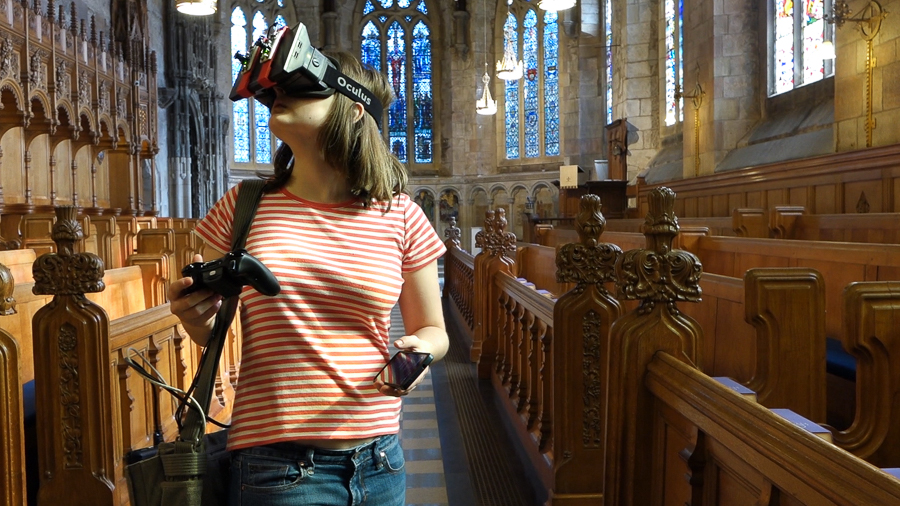
\includegraphics[width=\textwidth]{participant-f-3.jpg}
		\caption{The \textit{Mirrorshades} parallel reality platform in use.}
		\label{participant-f-3.jpg}
	\end{center}	
\end{figure}









%=========================================================================================================
%=========================================================================================================

Extended example goes here at the beginning.

%=========================================================================================================



Talk about history of alternate realities, talk about the disappointment of VR in the 90's \& it's resurgence now thank to Oculus, etc.






Alternate realities have been a mainstay of both popular science fiction \& of serious academic research, the concept of the existence of another `there' \& how we could visit it or bring it into our `here'
keeping authors \& scientists alike fascinated for many decades.

From the `Sensorama' simulator of the 1960s to the Oculus Rift of the early 2010s

From William Gibson's `The Gernsback Continuum' \& beyond through contemporary cyberpunk literature

the `gargoyles' of MIT


The 90's saw a surge of hype over the Virtual Reality concept, however with hardware \& software not ready to meet the expectations sown among consumers by the media the bubble burst.

The advent of the smartphone lead to the dissemination of any number of Augmented Reality, an attempt to merge to some extent our real world with aspects of the virtual.


And the Media Lab invented what they would call Cross Reality that linked a real world location with a virtual other via sensors \& actuators, such that an inhabitant of one could glimpse a tantalizing insight into the goings on of the `other' although they could not see into it.

This thesis explores an alternate reality that as yet has received little attention or even a name. Parallel Reality as it came to be called builds upon the concept of Cross Reality \& its two distinct environments each `complete unto itself'. But instead of the shadow of one environment only laying upon the other by manner of sensors \& actuators, new VR technology combined with indoor positioning systems allow a user to switch between environments - to at one moment view their RW surroundings \& at the next to view the equivalent vantage in a parallel virtual environment

%=====================
%On why alternate realities are predominantly visual?

\textit{``visual ordination of intellectual knowledge''}

\textit{``Seeing remains an insistent metaphor for all of cognition only because while the ocular lobes are merely one of our brain's tentacular connections to reality, they are among the most `conscious' of their capacity for information control.''}

The Mediated Sensorium, Caroline A. Jones



Caroline A. James speaking on the work of Janet Cardiff \& George Bures Miller

\textit{``Cardiff brings segmentation into the present, crafting `sound walks' that layer an alternate reality over the fl\^aneur's perambulations - a fantastic elaboration of the kind of personal soundscape chosen by the iPod user.''}


\textit{``Sight plays such a prominent part in the mental life that the field of vision is sometimes considered almost synonymous with the field of attention.''}~\cite{Lucas1951}

%=========================================================================================================

Structure of thesis here

% ======= ======= ======= ======= ======= ======= =======

\chapter{Extended Example}
\begin{quote}
	\textit{``There's no there, there. They taught that to children, explaining cyberspace.''}
\end{quote}
\hfill \textit{Mona Lisa Overdrive, William Gibson}
\\
\\
\\

%=========================================================================================================
%=========================================================================================================

%\begin{itemize}
%	\item \textbf{Content -} Short (10 pages is probably far too long) example or usage scenario of how the concepts investigated in the thesis have/could be used (a `near-future usage scenario').
%	\item \textbf{What has been done -} Nothing.
%	\item \textbf{What is left to do/how long should it take -} Come up with a legitimate scenario, keep it short, should probably be written after the bulk of the later sections so there's a clear idea of what scenario I actually want to allude to. Perhaps a few days writing.
%\end{itemize}

%\hrule

%\vspace{10mm}

\textbf{***Second Earth parallel reality example, think about what that person at DEMOfest was saying about being able to walk around Paris \& at any moment/location to transition into what it was like in the past.}

\textit{``The implication of HR is that, wherever you are, you can always be somewhere else''} - HyperReality p149

% ======= ======= ======= ======= ======= ======= =======

\chapter{Background, Theory \& Rationale}
\graphicspath{ {03_background/images/} }
\begin{quote}
\textit{``Where are you?'' Hiro says.
\\
\\
``In Reality or the Metaverse?''
\\
\\
``Both.''}
\end{quote}
\hfill \textit{Snow Crash, Neal Stephenson}
\\
\\

%=========================================================================================================
%=========================================================================================================

\label{chapter-background}

% 'Position' section from experimental plan document

%\section{Introduction}

This chapter explores the ecosystem of alternate realities, studying models that have been introduced to define and distinguish between different categories of alternate reality, producing a well defined taxonomy of alternate reality terms and introducing a model for illustration of alternate reality experience. Parallel reality is introduced into this theoretical framework as a new category of alternate reality, as the combination of a real and a virtual environment in a manner that allows the user to freely switch between them wherever within them they may be is not fully encapsulated by any of the existing definitions.




%The combination of real and virtual environments in this manner is not fully encapsulated by any previously defined alternate reality terminology, thus it was necessary to explore the ecosystem of alternate realities in order to correctly frame the introduction of a new category in relation to previously established models.

%The closest existing label is that of cross reality, but where cross reality sought to address the vacancy problem by means of sensor and actuator infrastructure, allowing actions in one environment to manifest into the other, the concept introduced by this thesis instead adopts the approach of direct visual engagement with both constituent environments.





%This research centres around the design, development and evaluation of a hardware and software platform which allows its user to observe and move around their Real World (RW) environment whilst wearing a wide field of view (FOV), stereoscopic 3D, Head Mounted Display (HMD) which allows them to alternatively view an immersive Virtual Reality (VR) environment from the equivalent vantage point. This is achieved by combining a head-tracked HMD, webcams, an indoor positioning system (IPS) and a 3D game engine, into a mobile \textit{cross reality} (XR) interface.

%One of the distinguishing features of XR is that, by linking real and virtual environments more closely, it mitigates the `vacancy problem': \textit{``the noticeable and profound absence of a person from one world, either real or virtual, while they are participating in the other''}, which arises \textit{``because people do not currently have the means to be in more than one place (reality) at a time''}~\cite{Lifton2007a}.

%Previous XR research approached the vacancy problem by integrating sensor/actuator networks into the environments, such that actions in one could manifest in the other, however direct visual engagement with the virtual environment was only possible from static interfaces at pre-determined locations within the real environment~\cite{Lifton2007a, Dublon2011}. The platform discussed in this document addresses this shortcoming by providing a mobile interface for visual engagement with both environments of a XR system, allowing the user to transition between viewing their real environment and a virtual environment at any time while maintaining the freedom to move around them, multiplexing visual stimuli from their real surroundings and from a parallel, virtual `mirror world'~\cite{Gelernter1993}.

%=========================================================================================================
%=========================================================================================================

\section{Defining Alternate Realities}

Alternate realities, explored in the context of this thesis as any situation in which the environmental stimuli received by a subject have been somehow modified or mediated (often by computer), have received substantial attention in recent decades. These themes have been explored for purposes as diverse as education~\cite{Warburton2009} and new forms of data visualisation~\cite{Coleman2009} to medical~\cite{TenEyck2011} and military training~\cite{Qiu2009} in addition to ever present entertainment applications~\cite{Scherrer2008}. Although terms such as \textit{virtual reality} and \textit{augmented reality} are now relatively common, both in the scientific literature and in the mainstream press, definitions of alternate reality terms such as these have often been used in vague and even conflicting manners, thanks in no small part to the fundamental nature of virtuality itself.

\begin{quote}
	\textit{``It is a characteristic feature of virtuality that it causes puzzlement regarding its relation to reality''}~\cite{Brey2014}
\end{quote}

The need for a well formulated framework of terms and related definitions for different alternate reality concepts has lead to several models that attempt to facilitate better understanding of the distinctions between different categories of alternate reality, most prominent among them the work of Milgram and Kishino in introducing the taxonomy of the reality-virtuality continuum. Not all of these frameworks have agreed upon their definitions of certain categories however, and in some instances there are even cases of contradiction.

%=========================================================================================================

\subsection{Milgram and Kishino's Reality-Virtuality Continuum}
\label{milgram&kishino}
Milgram and Kishino addressed the issue of alternate reality definitions in detail and can be accredited with introducing the terms \textit{augmented virtuality} and \textit{mixed reality} to the literature, prompted by their identification of the need for more encompassing terms to supplement the existing definitions of augmented reality~\cite{Milgram1999}.

%However despite these thorough and well-reasoned definitions being published originally in 1994, much of the subsequent literature studied for this review has adopted conflicting, or at least confusing and misleading, definitions.

One of the overbearing concepts introduced by Milgram and Kishino is that whilst both purely real and purely virtual environments do exist they should not be considered discrete alternatives but rather poles lying at opposite ends of a linear scale that stretches from an entirely real environment at one extreme to an ontologically parallel but entirely virtual environment~\cite{Qvortrup2002} at the other: the \textit{Reality-Virtuality continuum} (figure \ref{reality_virtuality_extent_of_world_knowledge_continuum}, top). The location of an environment along this continuum coincides with its location along a parallel \textit{Extent of World Knowledge continuum} (figure \ref{reality_virtuality_extent_of_world_knowledge_continuum}, bottom), where `world knowledge' refers to the amount of quantitative information that is associated with the content being presented to the user, or in other words how much of the environment is being `modelled' by a computer system.

\begin{figure}[h]
\centering
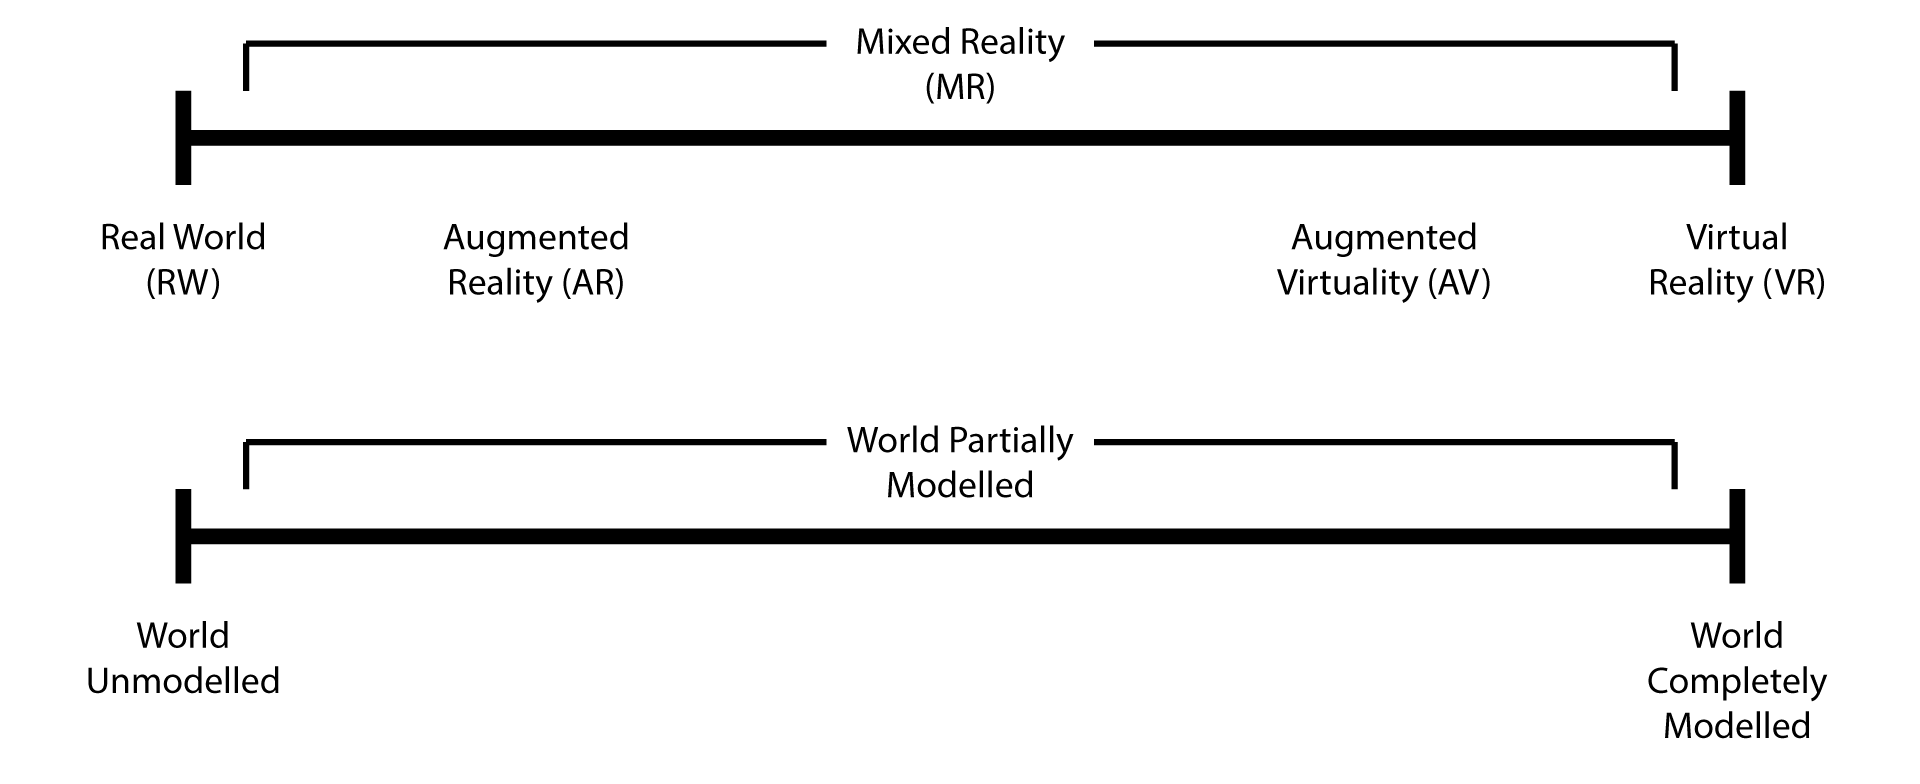
\includegraphics[width=\textwidth]{virtuality_continuum_extent_of_world_knowledge_continuum.png}
\caption{Milgram and Kishino's reality-virtuality continuum and extent of world knowledge continuum.}
\label{reality_virtuality_extent_of_world_knowledge_continuum}
\end{figure}

With a purely virtual environment, the entire viewport must necessarily be computer modelled in order to be rendered and as such there is complete quantitative information about and between all objects being presented. At the opposite end of the continuum with a completely real environment where none of the viewport is computer modelled there is no quantitative information associated with the content being displayed. At any point between the extremes the environment consists of a mixture of some modelled and some non-modelled content, with the computer associating quantitative information to, and between, the virtual objects, but not necessarily to the real objects or between the virtual and real objects.

Carrying the continuum concept further, Milgram and Kishino illustrated their understanding of augmented reality and also introduced two new related terms; augmented virtuality and mixed reality. Mixed reality describes any environment that is neither completely real nor completely virtual; that is, it encompasses all positions on the continuum between the extremes. Augmented reality is used to describe a real environment upon which virtual objects are overlain and augmented virtuality is used to describe a virtual environment upon which objects sampled from the real world (such as video feeds) are overlain. Both augmented reality and augmented virtuality are encompassed by mixed reality.

An obvious question raised from studying this figure is at what point toward the centre of the continuum an environment changes from being augmented reality into augmented virtuality or vice-versa. The answer to this question lies with consideration of what `background' environment is receiving the augmentations.

If one were to take a viewport depicting a purely real environment and incrementally add more and more virtual objects, the environment's classification might intuitively seem to progress rightward along the continuum. Eventually, with the majority of the real environment obscured by virtual objects one might posit that the resultant environment should have passed the centre point of the continuum and come to rest somewhere in its right half, gaining the classification of augmented virtuality. Likewise if one were to take a viewport depicting a purely virtual environment and incrementally introduce more sampled real objects to it, one might posit that it would eventually pass the centre point of the continuum and come to rest in the territory of augmented reality.

Anthony Steed's extension to Milgram and Kishino's reality-virtuality continuum concept clarifies the fallacy in this thinking by explicitly illustrating the concept of the `primary environment':

\begin{quote}
\textit{``While it is quite clear that the intention of plotting this axis was not to claim that it was actually a continuum between real and virtual, it is nevertheless clear that the main `environment' could be one of three things: a purely virtual environment, the local environment, or a remote real environment\footnote{Telepresence~\cite{Sheridan1992a}.}. One can think about what the background of the environment that the users see is...''}~\cite{Steed2014}
\end{quote}

Considering the first case of taking a viewport depicting a real environment and incrementally adding more virtual objects to it, the resultant environment is necessarily always augmented reality as the primary environment, that is the background upon which the augmentations are being placed, is real. Similarly in the second case the resultant environment is necessarily always augmented virtuality, as it is a virtual background environment that is the subject of the augmentations.

%=========================================================================================================

\subsection{Steve Mann's Venn Diagrams}
\label{stevemannvenn}
Steve Mann, the \textit{``father of wearable computing''}\footnote{\url{http://www.theguardian.com/technology/2012/apr/05/google-project-glass-digital-goggles}} and one of a group of researchers at MIT that became known as `cyborgs' for their body-worn computers and always-on Internet connections~\cite{Turkle2011}, presented a Venn diagram to illustrate the relationships between the different categories of alternate realities, when reviewing the problems that arise with existing taxonomies in  discussion about reality-modifying devices. Mann clarifies the use of the term `mediated reality' as \textit{``\ldots\ a general framework for artificial modification of human perception by way of devices for augmenting, deliberately diminishing, and more generally, for otherwise altering sensory input''}~\cite{Mann2002a}. Mediated reality thus encompasses all of mixed reality, but also the group of \textit{modulated reality} which covers devices such as eyeglasses that use lenses/mirrors to invert the wearer's view, but do not apply computer mediation or modification nor necessarily add or remove any content.

%Alone Together p 151

In this thesis, where we are concerned with alternate realities as those that are created or modified through means of computers or other apparatus (Mann's `devices'), one might want to consider the terms mediated reality and alternate reality to be one and the same. However in the larger consideration of virtual worlds as quoted in section \ref{intro-parallel-reality}, one might wish to reserve mediated reality specifically for the sub set of experiences that rely upon the application of `devices', whilst the super set of all alternate realities would contain in addition those experiences of simple imagination, storytelling and psychoactive agents.

Mann's Venn diagram (figure \ref{Mann_venn_original.png}) places augmented reality as a subset of mixed reality, but then further places virtual reality as a subset of augmented reality and in turn mixed reality, a decision not in fitting with Milgram and Kishino's definitions nor with logical deduction. A modified version of this diagram (figure \ref{Mann_venn_mod_1.png}) removes virtual reality from this position, as although virtual reality is by definition mediated, it is not necessarily always presented as part of an augmented or mixed reality, as purely virtual environments can and do exist. Mann himself states that \textit{``mixed reality exists in many forms along a continuum from augmented reality \ldots\ to more recent efforts at augmented virtuality''}, which is arguably contrary to his diagram's representation of virtual reality as a subset of augmented reality and in turn of mixed reality. Furthermore the modified diagram introduces augmented virtuality in Milgram and Kishino's definition, mentioned by Mann in his prose but not included in the original diagram. An overlap is also introduced here for those modulated reality environments that are also classified as mixed reality, as it is perplexing to think of a mixed reality environment that is neither augmented reality nor augmented virtuality (at least when considering a wholly real environment and a wholly virtual environment as the logically possible extremes, as in the reality-virtuality continuum and Steed's concept of primary environments).

\TwoFig{Mann_venn_original.png} {Mann's Venn diagram of alternate realities.} {Mann_venn_original.png}
       {Mann_venn_mod_1.png} {Mann's Venn diagram of alternate realities after modification.} {Mann_venn_mod_1.png}

\begin{figure}[h]
\centering
  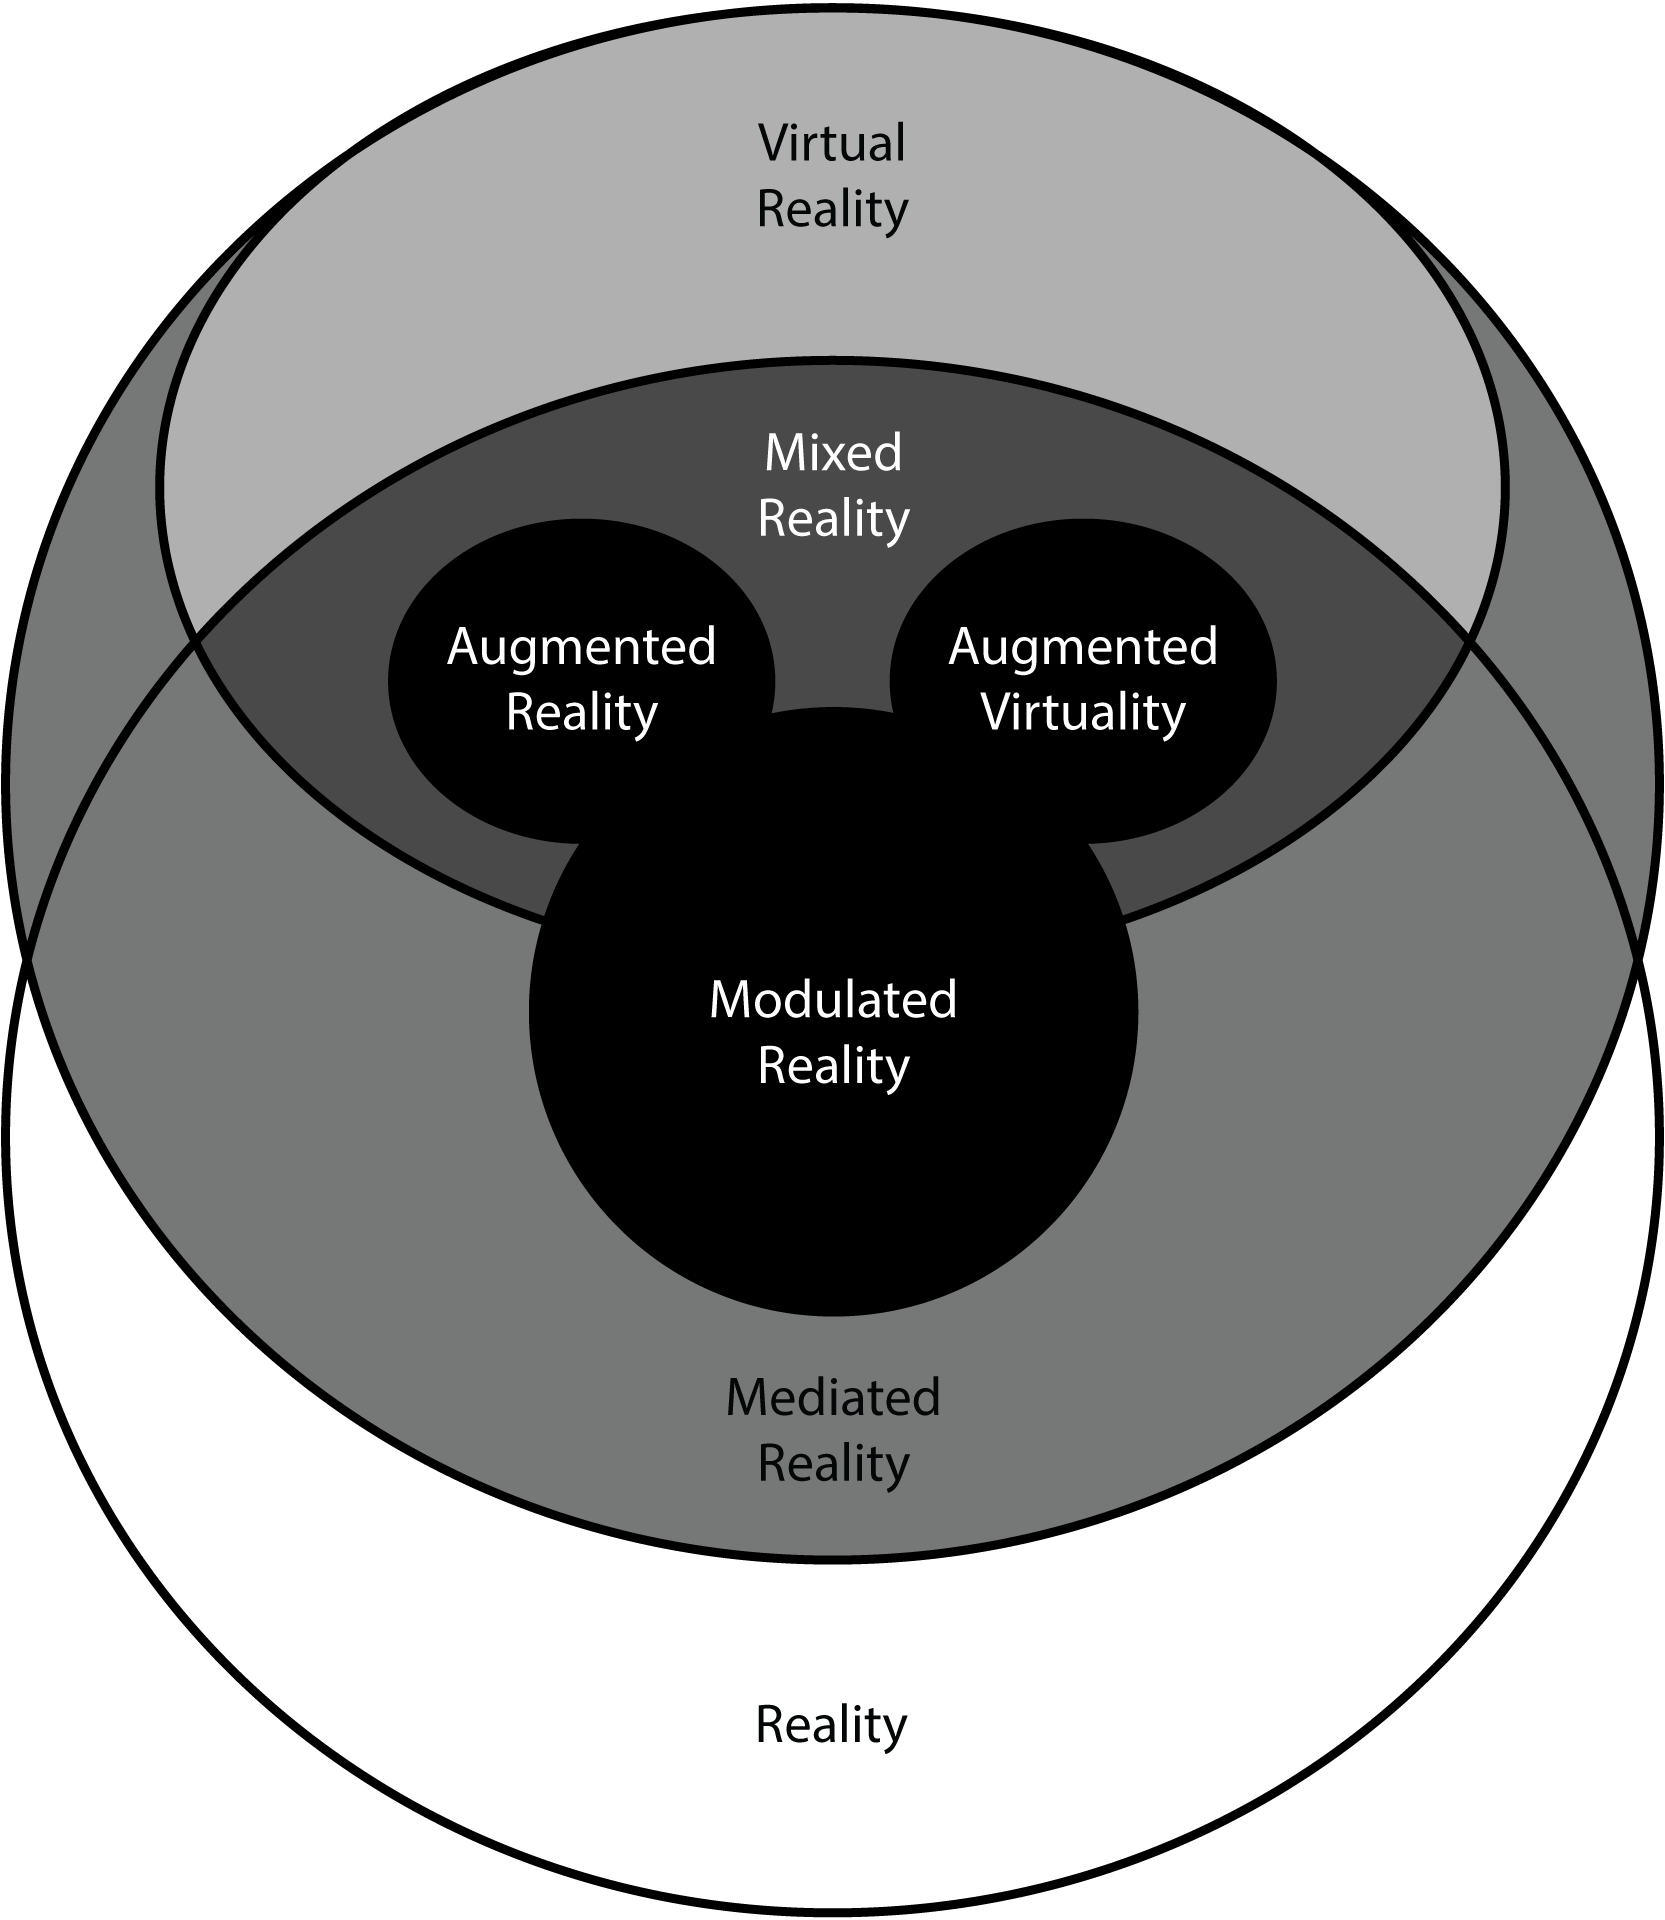
\includegraphics[width=0.5\linewidth]{Mann_venn_mod_3.png}
  \caption{Mann's Venn diagram of alternate realities after further modification.}
  \label{Mann_venn_mod_3.png}
\end{figure}

Visualising the position of the primary environments, reality and virtual reality, using this same method requires more drastic alteration to the diagram, but is diagnostic in further revealing the relationships between the terms covered in Mann's literature. The further modified Venn diagram (figure \ref{Mann_venn_mod_3.png}) shows that:
\begin{itemize}
	\item Mixed reality is the intersection of reality and virtual reality.
	\item Mediated reality can be comprised from purely real or purely virtual content.
	\item All virtual reality is necessarily mediated.
	\item Modulated reality can comprise only mediated real, or both real and virtual aspects in a mixed reality.
	\item Augmented reality and augmented virtuality can feature in modulated reality systems.
\end{itemize}

This final iteration of the Venn diagram still contains ambiguity, however it is more diagnostic for categorising the majority of alternate reality terms than the previous two diagrams, whilst also avoiding over-complication. There are two ambiguities to recognise. First, this diagram maintains from the original diagram those positions in which a system can exist that is both mixed and modulated, but which is neither augmented reality nor augmented virtuality. Second, the diagram does not accommodate a purely virtual environment that is then modulated; whether such a system would ever be created is debatable, as any modulation that could be performed by modulators external to the virtual environment implementation could almost certainly be better performed by that virtual environment implementation itself.

%=========================================================================================================
\subsection{Roy Want's Virtuality Matrix}
\label{roy-wants-virtuality-matrix}
Another method of illustrating the relationships between different categories of alternate realities was put forward by Roy Want in his introductory article for a 2009 issue of IEEE Pervasive Computing dedicated to the cross reality paradigm~\cite{Want2009}. He presents a 2x2 matrix categorising the different terms according to whether the experience and overlay data are real or virtual (figure \ref{Want_virtuality_matrix_original.png}). Whilst this is a useful representation, some of the definitions and criteria depicted do not match with those of Milgram and Kishino or even with those of other authors in the same issue of Pervasive, let alone other publications within the wider literature. This is a prime example of the importance of establishing an unambiguous set of definitions before embarking upon the path of introducing a new category of alternate reality. Figure \ref{Want_virtuality_matrix_modified.png} presents a modified version of this matrix that is in keeping with the framework laid out by Milgram and Kishino and the wider literature.

\TwoFig{Want_virtuality_matrix_original.png} {Want's virtuality matrix.} {Want_virtuality_matrix_original.png}
       {Want_virtuality_matrix_modified.png} {Want's virtuality matrix after modification.} {Want_virtuality_matrix_modified.png}

Where the original matrix positions cross reality in the upper left quadrant, at the congruence of `experience virtual' and `overlay data real', the modified matrix positions augmented virtuality. Referencing Milgram's continuum, `experience virtual' relates to a position somewhere within the right half, while `overlay data real' relates to presentation over this virtual primary environment of sampled real world data, resulting in a partially modelled environment, leaving us in the area of the continuum occupied by augmented virtuality.

The original matrix also features the term embodied virtuality in the upper right quadrant, at the congruence of `experience real world' and `overlay data real'. Want explains that this is an alternative term for \textit{ubiquitous computing} which is \textit{``essentially the opposite of VR''}. The modified matrix adopts the position that the opposite of virtual reality is simply reality and that ubiquitous computing does not constitute a category of alternate reality but rather a model of human-computer interaction (that can be implemented in either reality or augmented reality, depending upon how the ubiquitous computing infrastructure presents information to the user). A ubiquitous computing system is necessarily a real environment, as by definition it is the integration and dissemination of computational infrastructure into our real surrounds~\cite{York2004}. However whether this real environment is augmented by virtual objects is not restricted by the concept.

Finally the modified matrix removes the central mixed reality section from the original matrix, as its position could be misleading. Taking the boundaries between the sections literally, the reader could be led to believe that a purely virtual reality environment can be considered mixed reality, which it is not. If one wished to picture the position of mixed reality upon the modified matrix, one would do better to picture it covering the area enclosed by the union of the augmented virtuality and augmented reality regions.

%=========================================================================================================

\section{Adopted Alternate Reality Definitions}
\label{summaryofalternaterealitydefinitions}

Table \ref{adopted-alternate-reality-definitions} presents the basic categories of alternate reality and their definitions as a product of the survey and update of the frameworks explored thus far. This table does not claim to present an exhaustive list of \textit{all} categories of alternate reality; rather, it presents the fundamental set of common categories that are required to move forward with the framing of parallel reality in a well grounded fashion. Terms such as HyperReality~\cite{Terashima2001} (capitalization important, to differentiate from the postmodern term `hyperreality'~\cite{Baudrillard1994}) are intentionally excluded due to their limited applications and exposure in the literature.

%HyperReality (HR) is the term given to a hypothetical communications infrastructure that allows the seamless commingling of reality and virtual reality, human intelligence and artificial intelligence. In terms of the previously explored alternate reality terms, a HR system is most accurately described as facilitating the creation of mixed reality environments that bring virtual reality content into real world locations $-$ \textit{``It seeks to make virtual reality something that is experienced as part of physical reality, so that virtual and real phenomena appear to interact with each other: HR is VR as well as, not instead of, PR''}~\cite{Terashima2001}.

%HR is an abstract, high level term that refers to a category of mixed reality environments that combine VR content with views of the real world in a manner that arguably falls under the moniker of augmented reality, however HR places emphasis on the integration of the virtual reality content into the real world in a seamless manner, such that HR enables hyperreality (this latter non-capitalised term referring to the postmodern usage of the word wherein an observer is unable to distinguish reality from a simulation of reality~\cite{Baudrillard1994}).

%=========================================================================================================

\newpage

\begin{center}
\begin{longtable}{ l p{10cm} }

\toprule

\textbf{Term} & \textbf{Definition} \\

\midrule

%=========================================================================================================
		
Reality & An environment that is entirely unmodelled, with the viewport containing no virtual objects and with no computer-based quantitative information associated with any of the (necessarily real) objects. One of the fundamental primary environments, occupying an endpoint of the reality-virtuality continuum. \\
		
\midrule
		
%=========================================================================================================

Alternate Reality & Any environment in which the environmental stimuli received by a subject have been somehow altered or changed. That is, alternate reality is a term that encompasses everything that isn't simple `reality'. \\

\midrule
		
%=========================================================================================================

Mediated Reality & \textit{``A general framework for artificial modification of human perception by way of devices for augmenting, deliberately diminishing, and more generally, for otherwise altering sensory input''}~\cite{Mann2002a}. Encompasses all of mixed reality and modulated reality. \\

\midrule

%=========================================================================================================

Modulated Reality & Platforms that aim to modify the user's view, by multiplicative, diminishing, rotational, etc. techniques, where the user's view can be wholly real, or a mix of real and virtual content, not necessarily adding or removing anything. \\

\midrule

%=========================================================================================================

%Telepresence & The ability for a user to experience a sense of presence at a real location remote to themselves~\cite{Sheridan1992a}. \\

%\midrule

%=========================================================================================================

Mixed Reality (MR) & The broad range of environments that arise from the merging of real and virtual environments to some extent, such that the result is neither entirely real nor entirely virtual, with real and virtual objects co-existing. Both augmented reality and augmented virtuality are included under the broader classification of mixed reality. \\

\hline
		
%=========================================================================================================

Virtual Reality (VR) & The polar opposite of reality, an environment that consists solely of virtual objects, with computer-based quantitative information associated with and between all of them, creating a completely synthetic world entirely discrete and separate from the real world; a new world that exists solely within the data structures of a computer~\cite{Milgram1999, Want2009}. One of the fundamental primary environments, occupying an endpoint of the reality-virtuality continuum. \\

& While traditional definitions of virtual reality require the environment to be completely immersive, such that when involved with the environment the user is completely unaware of the real environment that surrounds them (such as by using HMD and body tracking techniques to remove logical anchors to the real world\footnote{\url{http://www.techcastglobal.com/documents/10193/34869/++Aaron/aade1a72-900b-4261-9214-061fba89053d}}) one can also adopt less drastic criteria and classify the virtual environments presented by video games viewed via traditional computer monitors as rudimentary implementations of virtual reality - \textit{``a virtual reality accessed through standard personal computers is arguably very much in evidence in computer games''}~\cite{Green2014}. \\
		
\midrule

%=========================================================================================================

%Distributed Virtual Reality (DVR) & Multi-user VR where telecommunications are employed to allow multiple (geographically distributed) users to occupy the same VR environment, allowing cooperation~\cite{Terashima2001}. \\

%\midrule
		
%=========================================================================================================

Augmented Reality (AR) & A mixed reality environment that features a real environment as its primary environment and onto which virtual objects are added or overlain. A common approach for achieving this addition/overlay is superimposing virtual objects over a direct or indirect view of the real environment using HMD \&/or cameras~\cite{Krevelen2010}, more recently making use of smartphones with their built in cameras and orientation sensing capabilities. \\

	%A commercial example of \textit{augmented reality} is the Layar browser for mobile phones, which overlays various forms of data onto the view captured by a phone's camera after determining its location and orientation using GPS, accelerometer and magnetometer readings~\cite{eishita:layar}

%~\cite{Milgram1999}

\midrule

%=========================================================================================================

Diminished Reality & Where augmented reality is concerned with adding virtual objects to a view of the real world, diminished reality is concerned with the removal of objects from a view of the real world~\cite{Mann2002}. Simple applications include the removal of real world advertisements, such as billboards. More involved applications might combine diminished reality with augmented reality to, for example, present a faithful representation of a historical scene upon a real world environment, by not just adding historical artefacts via augmented reality but also removing historically inaccurate later developments via diminished reality. \\

\midrule

%=========================================================================================================

Augmented Virtuality (AV) & A mixed reality environment that features a virtual environment as its primary environment and onto which sampled real objects are overlain, perhaps through the use of cameras~\cite{caballero:behand}. \\

%A simple commercial example of augmented virtuality is the EyeToy accessory and associated software for Sony's Playstation 2 games console (and later the Playstation Eye for the Playstation 3), a digital camera that captures images of players and their surroundings and integrates them into the gaming experience presented on the screen.

\bottomrule
\caption{Summary of alternate reality definitions.}
\label{adopted-alternate-reality-definitions}
\end{longtable}
\end{center}

%=========================================================================================================

%\section{Introducing a New Alternate Reality}



%=========================================================================================================

\section{Cross Reality}
\label{sec_crossreality}

\newcommand{\SLfootnote}{\footnote{Second Life.}}

With the sound understanding of the ecosystem of alternate realities provided by the preceding sections, parallel reality can now be introduced and situated accordingly. In order to do so, it is necessary to properly introduce one additional category of alternate reality, that of \textit{cross reality}. This is a more recent addition to the field of alternate realities, with its roots in the mid to late 2000s, than the more familiar terms covered in previous sections. However as one of its fundamental features is shared with parallel reality its inclusion in this discussion is required.

Cross reality (XR~\cite{kim:practical}) is a mixed reality situation that arises from the fusion of real-world sensor/actuator infrastructure with a complete virtual environment, facilitating synchronous bidirectional exchange of media and control information between real and virtual environments. Cross reality systems feature two environments, one real and one virtual, both complete unto themselves~\cite{lifton:merging} but enriched by their ability to mutually reflect, influence and merge into one another thanks to bidirectional information flow between them~\cite{kim:practical}. Sensors collect and tunnel dense real-world data into virtual environments where they are interpreted and displayed to dispersed users, whilst interaction of virtual participants simultaneously incarnates into the real world through a plenitude of diverse displays and actuators~\cite{Paradiso2009}, such that actions within the virtual environment can have `extravirtual effects'~\cite{Soraker2010} upon the real environment and vice-versa.

The principle features that distinguish cross reality from the other alternate realities covered so far are:
\begin{enumerate}
	\item A shift from single- to bi-directional information flow between real and virtual environments~\cite{kim:practical}.
	\item That both the real and virtual environments are complete unto themselves (but are enriched by their ability to mutually reflect, influence and merge into one another)~\cite{lifton:merging}.
\end{enumerate}

As an alternate reality paradigm cross reality has its roots in work undertaken by the IBM Virtual Universe Community\footnote{\url{http://eightbar.co.uk/2006/04/22/lessons-from-second-life/}}\footnote{\url{http://eightbar.co.uk/2006/04/09/second-life-outside-in/}}\footnote{\url{http://eightbar.co.uk/2006/04/04/well-it-got-my-attention-second-life/}}, described in personal correspondence with Ian Hughes:

\begin{quote}
\textit{``The control mechanisms worked two ways generally. There was a physical lab that had devices that were controlled by a pub/sub mechanism \ldots\ Those devices subscribed to various messages. So initially web pages controlled them \ldots\ Equally the objects generated messages when they were physically switched on and off. As SL\SLfootnote{} had an RPC interface it was possible \ldots\ to subscribe to the same messages and send requests into SL to change states of objects \ldots\ So there were lights, blinds, proximity detectors and even the tilt sensors on the laptops that were instrumented with these messages.''}
\end{quote}

It was the subsequent work of the Responsive Environments Group at MIT's Media Lab, centred around the research of Joshua Lifton in combining the Plug sensor/actuator platform~\cite{Lifton2007b} with a Second Life hosted virtual model of the physical Lab (shown in figure \ref{lifton_shadow_lab.png}) in the `Shadow Lab' project, that truly launched cross reality as an area of research potential. The Shadow Lab project did not allow for tandem visual engagement with both constituent environments of the cross reality platform, focussing instead on the interplay of sensor data and actuator commands exchanged between the environments. This visual aspect was addressed in part by the subsequent Ubiquitous Sensor Portal project, which situated 45 I/O rich `portals' (figure \ref{ubiquitous_sensor_portal.jpg}) throughout the Lab, each with a corresponding extension in Second Life. However in stark contrast to the Shadow Lab project, these portals were not situated in a simulation of the real Lab in situations corresponding to their physical location, but instead in an abstract virtual representation with a geometric layout reflecting intellectual affiliation as opposed to real-world location.

\TwoFig{lifton_shadow_lab.png} {Side view of the virtual Shadow Lab~\cite{Lifton2007a}, image courtesy Joe Paradiso.} {lifton_shadow_lab.png}
       {ubiquitous_sensor_portal.jpg} {A Ubiquitous Sensor Portal\protect\footnotemark , image courtesy Joe Paradiso.} {ubiquitous_sensor_portal.jpg}

\footnotetext{ \url{http://resenv.media.mit.edu/portals/} }

A potential source of standardization for the implementation of cross reality systems such as these that leveraged virtual world technology such as Second Life was presented by ISO/IEC 23005 (also referred to as MPEG-V), whose creation aimed to \textit{``enable the interoperability between virtual worlds \ldots\ and with the real world''} including through the use of \textit{``sensors, actuators, vision and rendering''}~\cite{InternationalOrganizationforStandardization2011}.

The concept of a bidirectional connection between real and virtual environments, but which did not remove the boundaries that defined them, was also the basis of the `interreality' concept, in which user behaviour in the real world would influence the virtual environment that was used as part of a neuropsychological rehabilitation program~\cite{Giuseppe2014a}.

%=========================================================================================================

\subsection{The Vacancy Problem}

One of the driving motivations behind Lifton's work was what he dubbed `the vacancy problem':

\begin{quote}
\textit{``the noticeable and profound absence of a person from one world, either real or virtual, while they are participating in the other. Simply put, the vacancy problem arises because people do not currently have the means to be in more than one place (reality) at a time.''}~\cite{Lifton2007a}
\end{quote}

The Shadow Lab addressed the vacancy problem via the sensor/actuator infrastructure, more closely linking the real and virtual environments such that actions and events in one could manifest and be observed by users in the other even if they could not directly visually observe both environments in tandem. The vacancy problem was previously observed by HyperReality researchers, touching on an observation of the polysocial situations observed among mobile phone users of the time as a manifestation of the problem even before virtual environments were introduced to the picture. %HyperReality p35

\begin{quote}
	\textit{``One of the main problems with \ldots\ virtual reality is what to do about the body that is left behind in physical reality \ldots\ In HyperReality a person by definition is perceptually aware of the physical world around them, yet part of the attention normally given to the physical reality is given to interacting with virtual reality. It is difficult as yet to see how much this matters, but the increasing use of the mobile phone, which is a primitive form of HR\footnote{HyperReality}, gives us some feel for the issues. People using a mobile phone can walk busy streets \ldots\ while talking to someone who is not there.''}~\cite{Terashima2001}
\end{quote}

%=========================================================================================================

\subsection{Alternate Reality Definitions from Cross Reality}

Lifton's use of alternate reality terminology does not directly conclude that mixed reality is a broad term encompassing both augmented reality and augmented virtuality, but defines it as an environment:

\begin{quote}
	\textit{``\ldots\ which would be incomplete without both its real and virtual components. For example, the walls and windows of a mixed reality house might be real, but the view out the windows might be virtual, either generated by a projector or as a blue screen effect in a head-mounted display. Without both the real house and the virtual views out the windows, the illusion of a consistent reality is broken''}~\cite{Lifton2007a}
\end{quote}

The diagram Lifton presents (figure \ref{original_lifton_axis.png}) alludes to Milgram's continua but places mixed reality, under the above definition, as a separate category of alternate reality between augmented reality and virtual reality. Lifton does not mention augmented virtuality, even though the cross reality systems he presents could arguably be considered as causing it to manifest. Figure \ref{modified_lifton_axis.png} is the result of modifying this diagram to match the definitions from table \ref{adopted-alternate-reality-definitions}.

\begin{figure}[h]
	\centering
	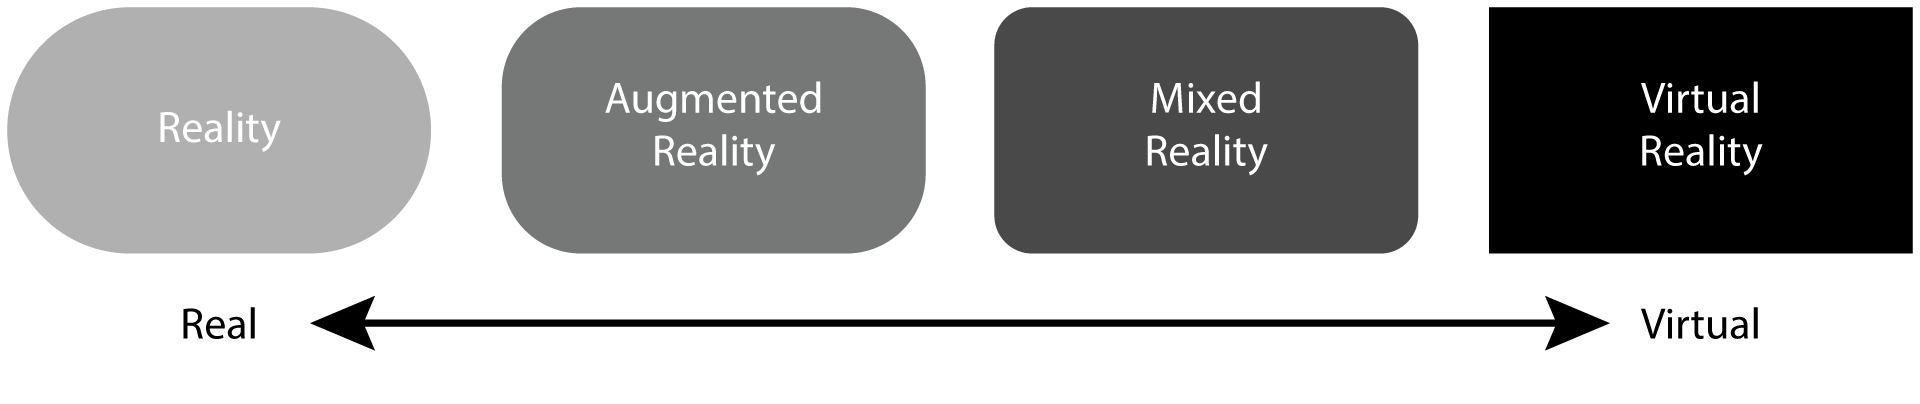
\includegraphics[width=.8\textwidth]{Lifton_continuum_original.png}
	\caption{Lifton's virtual worlds taxonomy.}
	\label{original_lifton_axis.png}
\end{figure}

\begin{figure}[h]
	\centering
	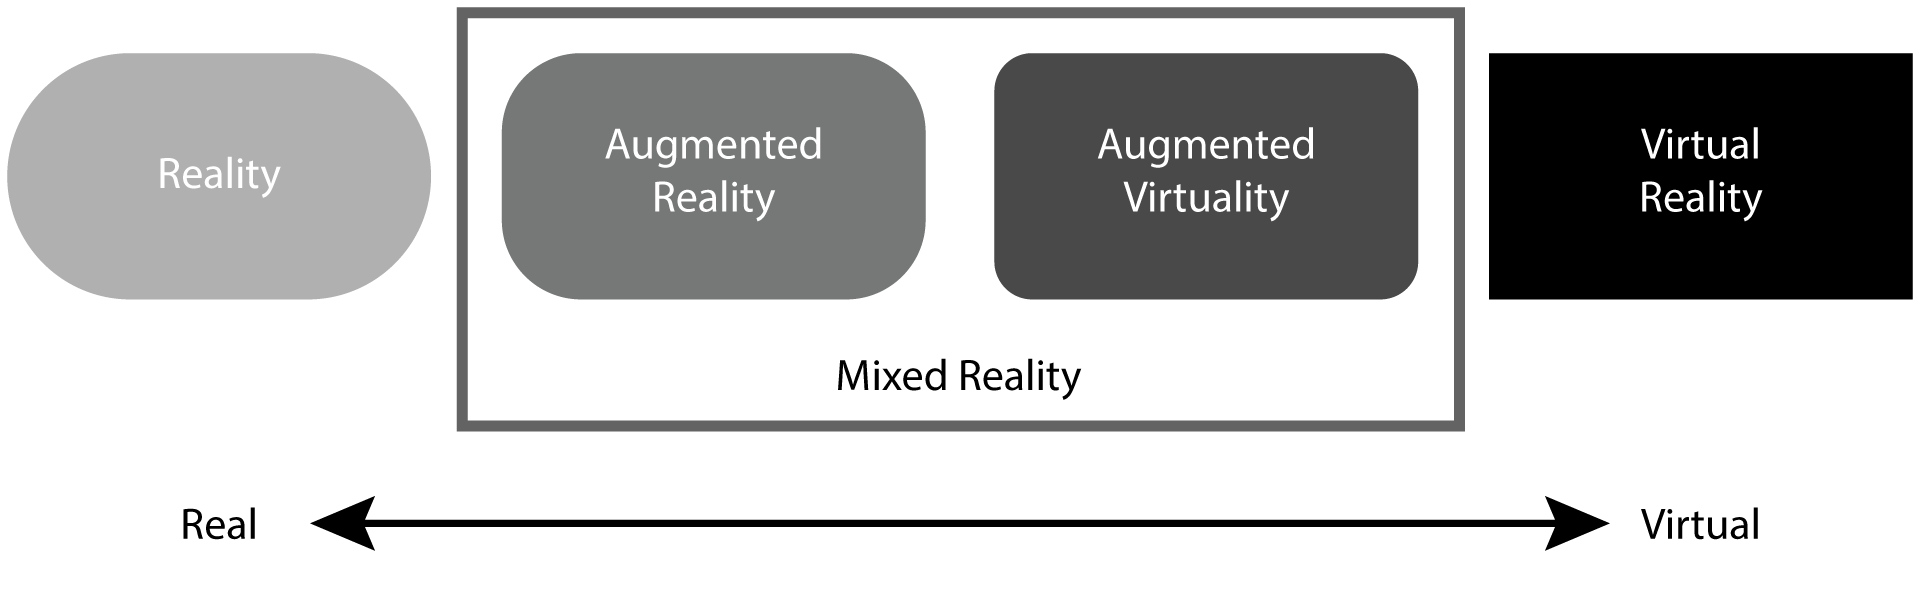
\includegraphics[width=.8\textwidth]{Lifton_continuum_modified.png}
	\caption{Lifton's virtual worlds taxonomy after modification.}
	\label{modified_lifton_axis.png}
\end{figure}

Lifton does however explain that while such a taxonomy can be successfully applied to most alternate realities, with each falling into a different singular category, it does not well address those that feature two complete realities, one real and one virtual, which is one of the distinguishing characteristics of cross reality. He instead presents figure \ref{reality_virtual_reality_sensor_networks.png} to show how sensor/actuator infrastructure causes the real and a virtual environment to merge into a cross reality situation.

\begin{figure}[h]
	\centering
	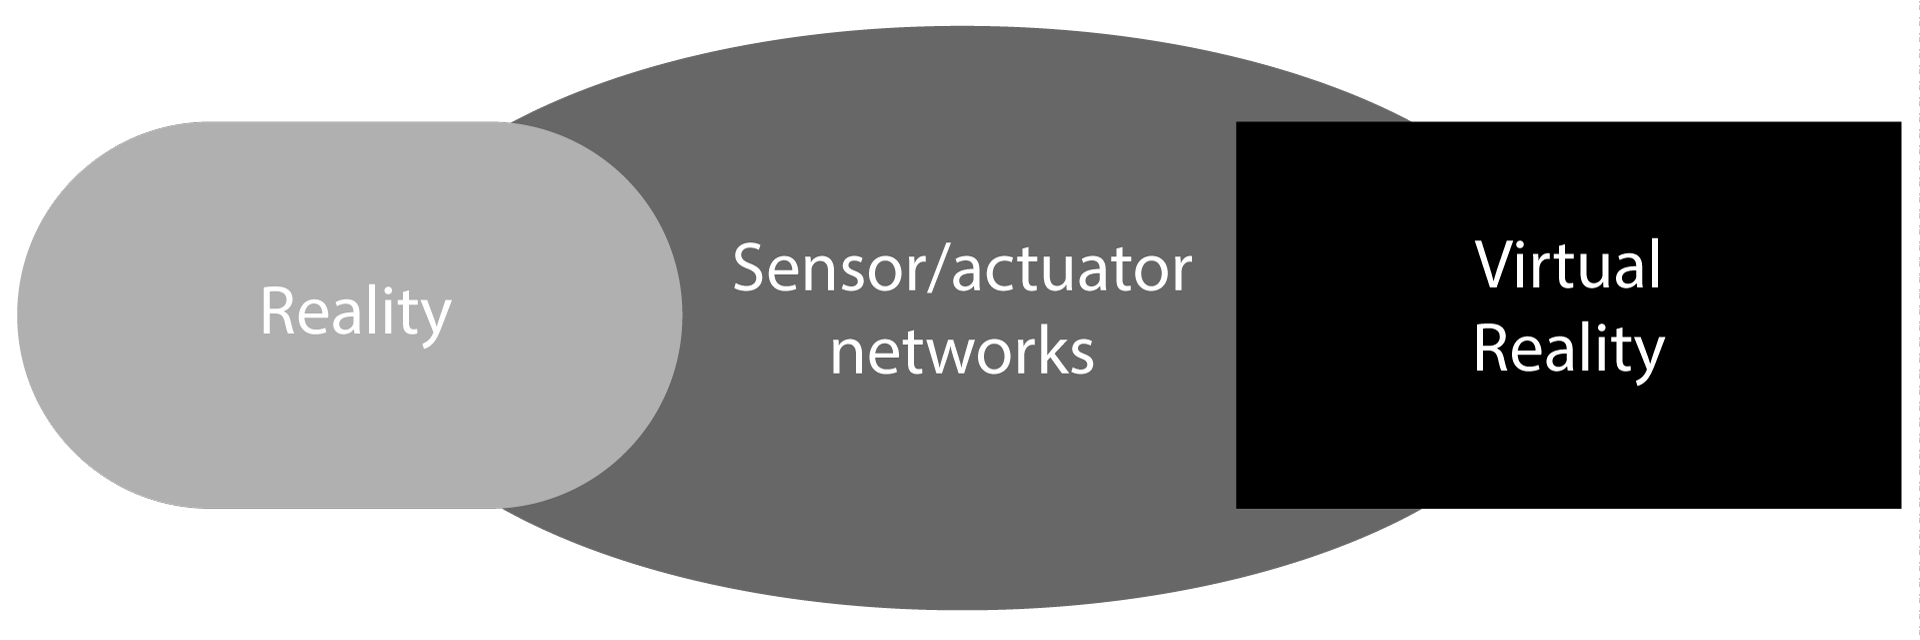
\includegraphics[width=.6\textwidth]{reality_virtual_reality_sensor_networks.png}
	\caption{Sensor/actuator infrastructure merging real and virtual environments into an instance of cross reality.}
	\label{reality_virtual_reality_sensor_networks.png}
\end{figure}

%page 37 of Lifton's thesis

%=========================================================================================================

\subsection{Position of Cross Reality}

\label{positionofcrossreality}

\newcommand{\avxrfootnote}{\footnote{This discussion over the relationship between augmented reality and cross reality also stands for the relationship between augmented virtuality and cross reality, however as augmented virtuality has received less attention in the literature and in commercially available implementations, the discussion uses augmented reality as its example.}}

The position of cross reality in relation to other alternate realities can be visualised using Milgram and Kishino's reality-virtuality continuum. As one of the defining characteristics of cross reality is that it features two environments, both complete unto themselves, the explanation herein distinguishes between environments themselves (depicted in figures \ref{virtuality-continuum-augmented-reality} to \ref{virtuality-continuum-cross-reality-information-flows-dashed.png} by solid ellipses) and where the environmental stimuli that the user is perceiving originate from (depicted by dashed ellipses).

%Ontology - The core meaning within computer science is a model for describing the world that consists of a set of types, properties, and relationship types. There is also generally an expectation that the features of the model in an ontology should closely resemble the real world (related to the object).

Of particular importance is to appreciate the distinction between a cross reality system and an augmented reality system\avxrfootnote{}, as both concepts involve user engagement with both real and virtual content. An augmented reality system features a single environment comprised of the user's real world overlain by and `combined' with~\cite{Billinghurst2014} some virtual content, a \textit{`` `cybrid' environment existing simultaneously in virtual and physical modes''}~\cite{Lichty2014}, with the user perceiving stimuli from this single augmented environment (figure \ref{virtuality-continuum-augmented-reality}). A cross reality system instead features two discrete environments, one real and the other virtual, each complete unto itself (figure \ref{virtuality-continuum-cross-reality-1}), with the user attending either to the stimuli originating from the real environment (figure \ref{virtuality-continuum-cross-reality-2}) or to the stimuli originating from the virtual environment (figure \ref{virtuality-continuum-cross-reality-3}).

\begin{figure}
	\begin{center}
		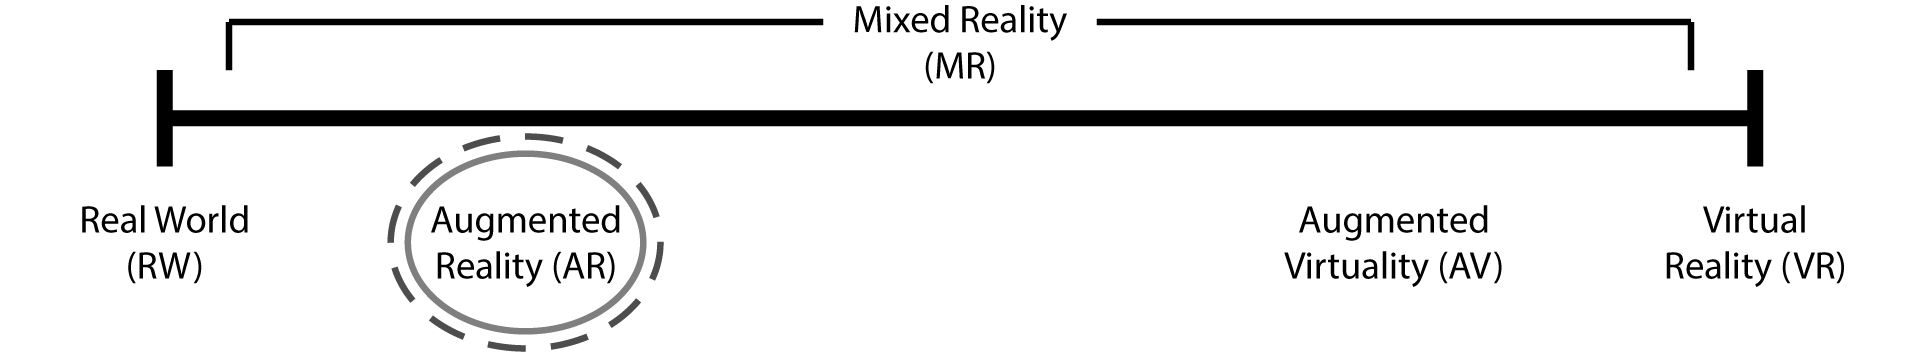
\includegraphics[width=\textwidth]{virtuality-continuum-augmented-reality.png}
		\caption{The single environment of an augmented reality system.}
		\label{virtuality-continuum-augmented-reality}
	\end{center}
\end{figure}

\begin{figure}
	\begin{center}
		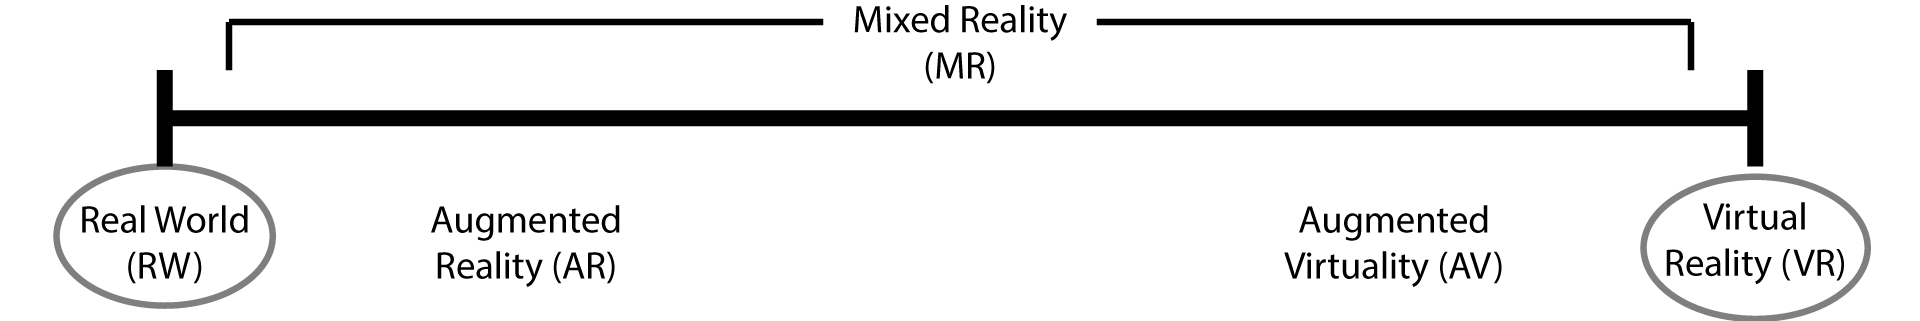
\includegraphics[width=\textwidth]{virtuality-continuum-cross-reality-1.png}
		\caption{The two environments that comprise a cross reality system.}
		\label{virtuality-continuum-cross-reality-1}
	\end{center}
\end{figure}

\begin{figure}
	\begin{center}
		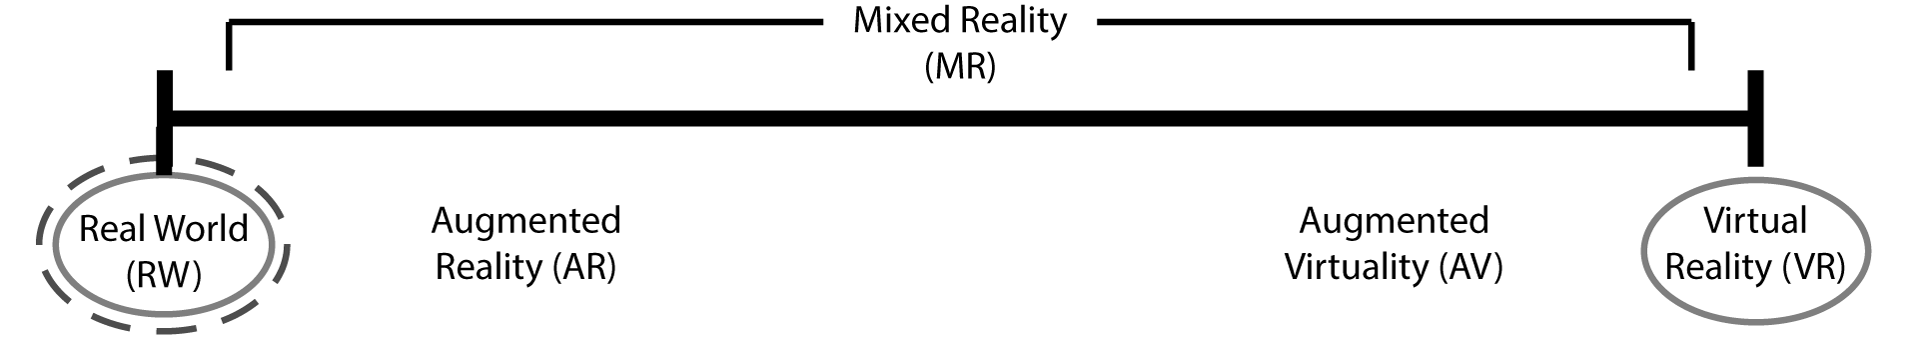
\includegraphics[width=\textwidth]{virtuality-continuum-cross-reality-2.png}
		\caption{A cross reality system with the user attending to real stimuli.}
		\label{virtuality-continuum-cross-reality-2}
	\end{center}
\end{figure}

\begin{figure}
	\begin{center}
		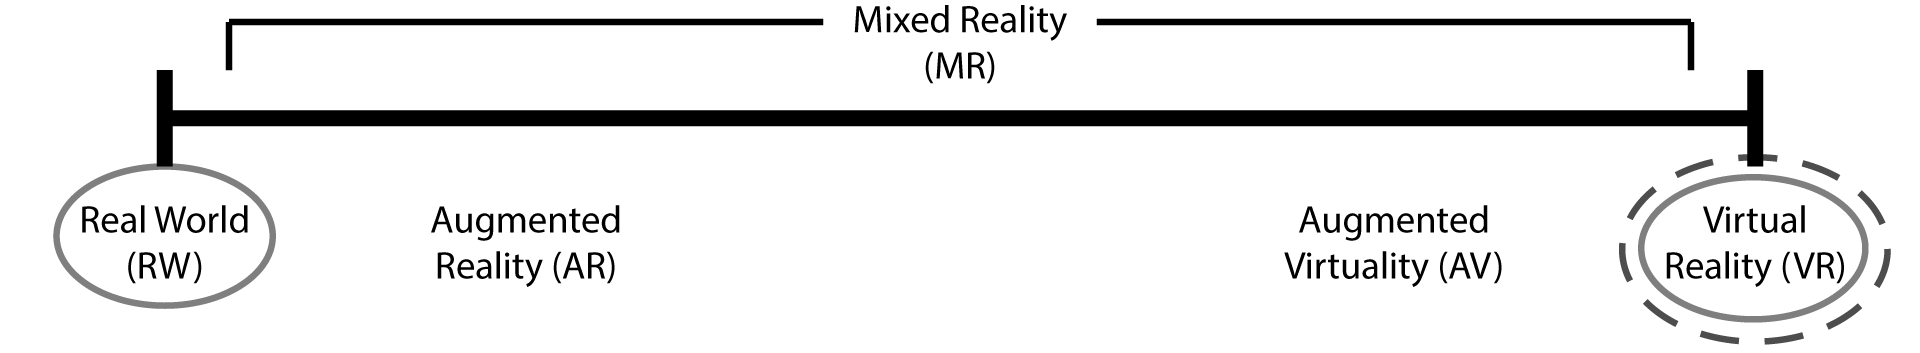
\includegraphics[width=\textwidth]{virtuality-continuum-cross-reality-3.png}
		\caption{A cross reality system with the user attending to virtual stimuli.}
		\label{virtuality-continuum-cross-reality-3}
	\end{center}
\end{figure}

%Similarly to AR, a HR environment likewise constitutes a single physical environment, formed by the seamless introduction of VR content into the real world, rather than two complete environments;

%`physical' quote is HyperReality p158

%HyperReality p26
%\begin{quote}
%	\textit{``\ldots\ virtual people, virtual objects and virtual settings can interact and thereby communicate with real people, real objects and real settings as though they were all part of the same world.''}~\cite{Terashima2001}
%\end{quote}

Although a cross reality system as a whole might be considered a case of mixed reality, whether each of its constituent environments should be considered outwith or within the realm of mixed reality (especially when visualised upon the continuum) is open to debate. Taking the real environment as an example, one could argue that the use of actuators to produce physically observable effects on behalf of controls from the virtual environment constitutes an augmented reality environment. However in adherence with the definition of augmented reality adopted in table \ref{adopted-alternate-reality-definitions} we would not label this an augmented reality environment as we do not have \textit{virtual} objects overlain upon our view of the real environment, but rather \textit{real} physical objects controlled by the actions and events within a discrete virtual environment. So whilst an augmented reality environment falls within the realms of mixed reality, the constituent environments of a cross reality system when considered individually are considered here as occupying the two extremes of the continuum, outwith the mixed reality region and thus their depiction as such in figures \ref{virtuality-continuum-cross-reality-1} to \ref{virtuality-continuum-cross-reality-information-flows-dashed.png}. It is beyond the scope of this chapter to discuss the ontological implications of the `reality' of virtual objects and actions, so the interested reader is referred to Brey~\cite{Brey2014} for further discussion of this subject.

%***this is more to do distribution of the dashed line surrounding the environments, rather than the position of the environments themselves (solid line)***

%However, XR systems that allow simultaneous interaction with both of their constituent environments blur this definition; using a XR platform such as that discussed in this document, a user can transition between perceiving stimuli from each of these environments (figures \ref{virtuality-continuum-cross-reality-2} and \ref{virtuality-continuum-cross-reality-3}) in a manner that allows them to engage with each environment without becoming wholly vacant from the other.

A further distinction between augmented reality and cross reality is made by consideration of Steed's primary environment concept. For an augmented reality system the primary environment is necessarily real, as augmented reality describes systems in which virtual objects are superimposed upon a view (a background) of a real environment. However for a cross reality system one could argue that the primary environment is either real or virtual, depending upon how the user interacts with the system. For the user that walks through the real environment of a cross reality system and views their unmediated surroundings (including physical actuations triggered by events within the virtual environment), one would intuitively posit that their primary environment is real. But for the user that sits in front of a computer monitor and uses an avatar to walk through the virtual environment of the same cross reality system and hence views the avatar's virtual surroundings (including visualisations of sensor data collected from the real environment), one would posit that their primary environment is virtual. Considering figures \ref{virtuality-continuum-cross-reality-2} and \ref{virtuality-continuum-cross-reality-3} again, one could say that the dashed ellipses thus represent the primary environment for a cross reality system in each of these scenarios respectively.

In relation to the vacancy problem, in scenarios wherein interaction with both real and virtual content is desirable but for which a complete virtual environment is not required, augmented reality circumvents the vacancy problem by virtue of presenting a single mixed reality environment to the user. However for scenarios wherein the use of a complete virtual environment is either beneficial or outright required, the vacancy problem must be mitigated to allow for constructive interaction with these two discrete environments; as is the aim of the cross reality paradigm.

%=========================================================================================================

\section{Parallel Reality}
\label{parallelrealityinbackground}
\newcommand{\PRfootnote}{\footnote{Note that the use of `PR' in the quotation in section \ref{subsec_HyperReality} is a reference to `physical reality' (that author's term for what this thesis simply calls `reality') and is not a reference to parallel reality.}}

The discussion in the previous section highlighted that the first distinguishing feature of cross reality that differentiates it from other alternate realities such as augmented reality and augmented virtuality, is that it features two discrete environments, one real and the other virtual. The second distinguishing feature is the presence of a bidirectional flow of information between these two environments. These features are visualised by figure \ref{virtuality-continuum-cross-reality-information-flows-dashed.png}.

\begin{figure}[h]
	\begin{center}
		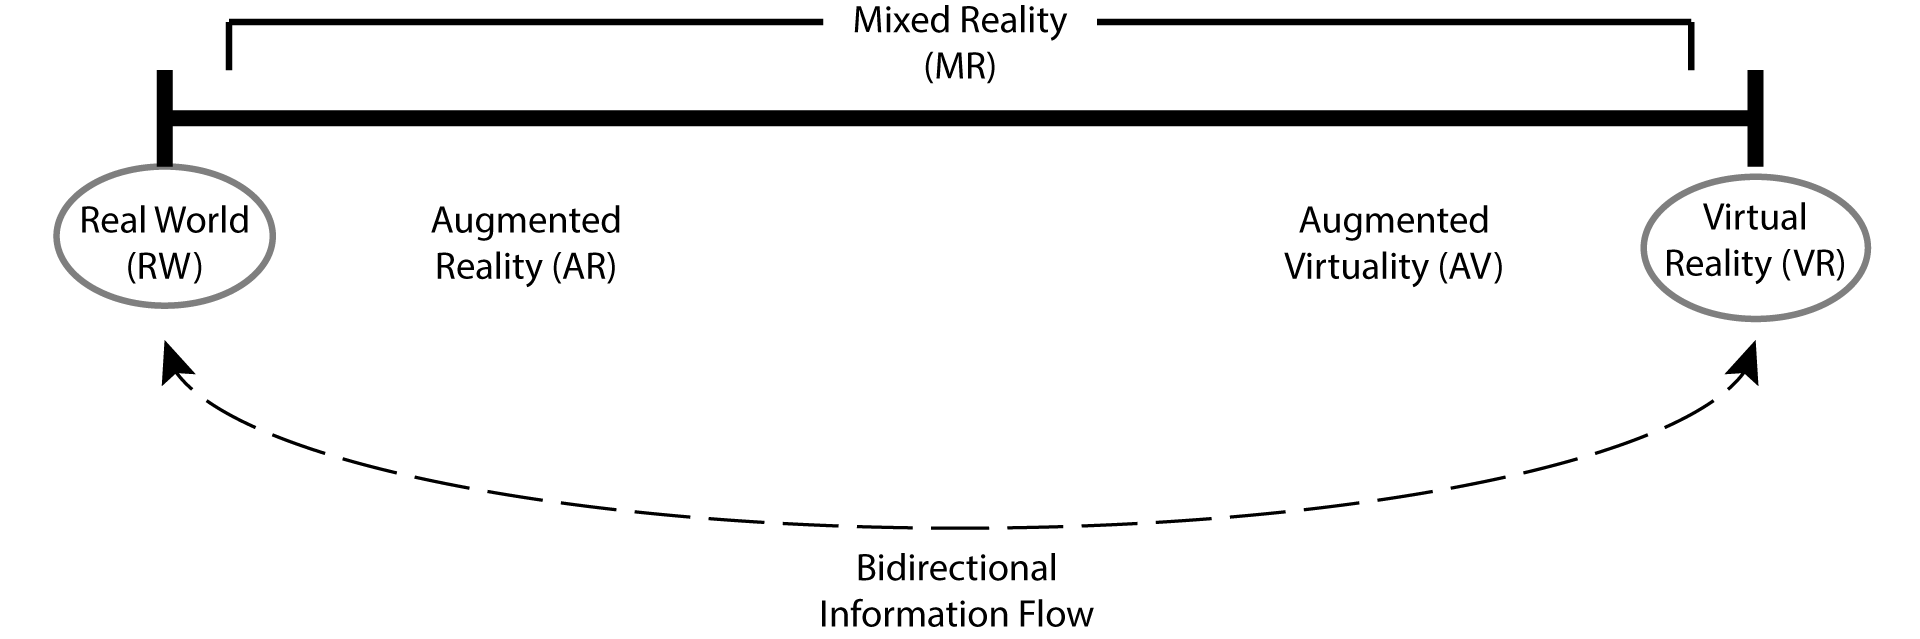
\includegraphics[width=\textwidth]{virtuality-continuum-cross-reality-information-flows-dashed.png}
		\caption{The two environments that comprise a cross reality system, with the bidirectional information flow between them.}
		\label{virtuality-continuum-cross-reality-information-flows-dashed.png}
	\end{center}
\end{figure}

While the parallel reality concept introduced by this thesis also features two discrete environments, one real and one virtual, that users can freely transition between visually observing, it does not feature this bidirectional information flow between the environments (other than using sensed real position information to maintain the user's vantage point into the virtual environment). Thus, this concept could not be considered cross reality as it does not meet both of the distinguishing criteria. The term \textbf{parallel reality} is instead proposed to describe the new concept. Parallel reality is thus defined as:

\begin{quote}
	\textbf{Parallel Reality:} A system comprising two environments, one real and the other virtual, each complete unto itself and wherein the user may freely switch between them.
\end{quote}

%Should a bidirectional information flow be introduced to a parallel reality system, or the ability to transition between receiving visual stimuli from either environment be introduced into a cross reality system, one would in effect produce \textit{parallel cross reality}.

Picking up the discussion of primary environments once more, if one follows the reasoning that the primary environment of a cross reality system depends upon the method with which the user interacts with the system, it stands that a parallel reality system can be described as one that provides the user with the ability to change this method and thus change their primary environment at will. In this regard we further distinguish a parallel reality system from an augmented reality system, by defining the former as allowing its user to switch between two different primary environments whereas the latter augments one particular primary environment.

%=========================================================================================================

\subsection{Spatial Equivalence in Parallel Reality}

\label{spatial-equivalence}

%(Life on the Screen, p219
\newcommand{\turklevrfootnote}{\footnote{\textit{``For virtual reality to be interesting it has to emulate the real. But you have to be able to do something in the virtual that you couldn't in the real.''}~\cite{Turkle1997}}}

When discussing a parallel reality system that allows a user to transition between two environments, one real and the other virtual, one must consider the relationship between the two environments, namely whether (and if so, to what extent) their layout, dimensions and content relate to each other, a consideration we will refer to as their \textit{spatial equivalence}.

This distinction depends partly upon whether one adopts a dualistic concept of virtual space experience, wherein `cyberspace' is a space in its own right with its own logic and metaphysics thus capable of playing host to any number of fantastical things and places, or whether one restricts the virtual environment by following a positivistic understanding of virtual space in which it serves only as a representation of real - using cyberspace for \textit{``creating acceptable substitutes for real \ldots\ environments''} instead of for \textit{``constructing imaginary worlds that are indistinguishable from the real world''}~\cite{Qvortrup2002}. One may also wish to consider this distinction in relation to the different stages identified by Baudrillard between simulacra and simulation, with complete spatial equivalence occupying the first stage, of a faithful image or copy of a profound reality (the positivistic position), zero spatial equivalence occupying the fourth stage, of pure simulation with no relation to anything in reality (the dualistic position), and partial equivalence perhaps occupying the second stage, a perversion of reality~\cite{Baudrillard1994}.

%=========================================================================================================

However one treats virtual space, a parallel reality system would be unrewarding if the real and virtual environments were identical\turklevrfootnote{}. However a virtual environment that shares roughly the same fundamental dimensions and layout as the real environment (representing the same `place') but which presents an \textit{alternative} representation of it has been proven to be a useful modality in previous cross reality research (see section \ref{sec_crossreality}) and it is this arrangement that this thesis explores; in particular where the virtual environment represents the same place as the real environment but at an earlier moment in \textit{time}. This concept of spatially equivalent real and virtual environments has recently been explored under the name `substitutional reality'~\cite{Simeone2015}, but without the ability to switch between the two environments.

One might consider the `Second Earth' concept to be the ultimate realisation of this scenario of spatially equivalent real and virtual environments. The combination of virtual world technology (as in Second Life) with `mirror world' technology (as in Google Earth), Second Earth theorises a virtual simulation/reconstruction of the entire physical world, such that for any location in the real world there is a corresponding location in the virtual world\footnote{\url{http://www.technologyreview.com/Infotech/18911/}}. The parallel reality platforms developed in this thesis focus on individual locations, however it does not take a great leap of the imagination to comprehend the worth of such a system scaled to larger, even global, application.

Although the use cases for parallel reality systems that feature completely unrelated real and virtual environments (including where the virtual environment is entirely fictitious) may seem limited in terms of possible benefits to understanding or knowledge gain when comparing and contrasting the environments, an educated approach to implementing transitions between these environments, that takes similar considerations as the platforms developed in this thesis, does conceivably have purpose. In the opening quote to this chapter, taken from Neal Stephenson's cyberpunk novel \textit{Snow Crash}, the protagonist enquires about the location of another character, both in the real world and in the `Metaverse' - analogous to a virtual world akin to Second Life, accessed via a HMD, comprised of entirely synthetic locations with no counterparts in the real world and which is used to accomplish the same tasks for which today we use the Web. Her response is that \textit{``In  the Metaverse, I'm on a plusbound monorail train. Just passed by Port 35.''} whilst in reality she is at a \textit{``Public terminal across the street from a Reverend Wayne's"}.

There is no spatial equivalence in this scenario between the real environment and the virtual environment; they are not the same `place'. However the protagonist still wishes to be able to experience both by transitioning between them, paying attention to one while travelling through the other. Situations of publicly experienced spatially equivalent and non-equivalent alternate realities are also rife in Vernor Vinge's \textit{Rainbows End}:

\begin{quote}
	\textit{``Robert leaned back from the window and reached out to wider universes. Colored maps appeareed before his eyes. These were realities that were geographically far away, not overlaid upon San Diego at all \ldots\ Finally he got a window that promised `public local reality only.' ''}~\cite{Vinge2006}
\end{quote}

While these situations are currently science fiction, recent developments in mobile VR platforms such as Samsumg Gear VR\footnote{\url{http://www.samsung.com/global/microsite/gearvr/}} hint that we are not so far away from a time in which members of the general public will wish to multiplex their real environment with a virtual one in this fashion while in public, in the same way that people commonly engage in computer-mediated communication (CMC) via their smartphones at the same time as walking through real environments and conversing with the people around them, creating instances of polysocial reality. If a parallel reality system were to allow interaction between its user and other virtual environment users who are not part of the parallel reality scenario, it is conceivable that polysocial instances would arise with parallel reality users socially engaging both with people in their immediate real environment and with people in their immediate virtual environment, even where the latter are not present in the former. This situation would present \textit{``\ldots\ instances of synchronous polysocial reality, multiple presence \ldots\ being activated in different environments.''}\footnote{Personal correspondence with Sally Applin, polysocial reality author.}

With the majority of players of popular Massively Multiplayer Online games (MMOs) wishing they could spend more time playing, over a fifth even wanting to spend all of their time in game~\cite{Castronova2006}, and with social roles and the community aspect constituting key aspects of these game's popularity~\cite{Castronova2006, Bartle2004}, informing the implementation of transitions between real and virtual in such systems with the findings of the experiments in this thesis into spatially equivalent parallel reality promises to be beneficial to the further development of 3D social CMC in a wider sense.

%=========================================================================================================

\subsection{The Case for Parallel Reality}
\label{caseforpr}
%ARCHEOGUIDE makes the point that AR is good because users are not isolated/completely immersed in a synthetic world - well Mirrorshades allows uers to more fully immerse themselves in a synthetic world, but without becoming isolated in it (eg without becoming ***vacant*** from the real world)

A parallel reality system that presents the user with the choice between immersive visual stimuli from both its constituent environments allows that user to engage with both real and virtual content in a manner that is similar to, but has a number of advantages over, previous alternate reality systems, including augmented reality implementations and cross reality systems:

\begin{itemize}
	\item A parallel reality system is less critical of registration (the accurate positioning/alignment) between real and virtual, as virtual objects are seen as part of a larger virtual environment instead of being rendered atop a view of the real environment~\cite{Azuma1997}.
	\item A parallel reality system can make use of existing virtual reality content without the overhead of decanting/extracting a subset of the virtual components into an augmented reality framework (e.g. manually selecting which objects within the virtual environment are to be displayed over the real environment).
	\item The use of a complete virtual environment allows virtual content to be more encompassing and immersive, allowing total control over lighting, shadows, reflections, particle effects, etc. which would be difficult or impossible for an augmented/diminished reality platform to render atop a view of a real environment.
	\item The vacancy problem is further addressed, but instead of doing so by linking real and virtual environments by sensor and actuator infrastructure, vacancy in both environments is alleviated by furnishing users with the ability to transition between perceiving visual stimuli from them both.
\end{itemize}

Parallel reality platforms are thus well suited to situations in which interaction with the visual stimuli of both real and virtual environments is required and where one or more of the following hold true:

\begin{itemize}
	\item In lieu of accurate registration between real and virtual, there is a strong focus on the virtual environment's atmosphere and immersion~\cite{deamicis:gamebased}.
	\item There is existing virtual reality content.
	\item The visual differences between real and virtual environments are substantial enough that an augmented/diminished reality system would resort to augment or diminish almost the whole real view. While augmented reality \textit{``smears an informational coating over real space''}~\cite{Andersen}, parallel reality presents a complete virtual environment. While augmented reality is beneficial where one wishes the juxtaposition of virtual objects upon what is already present in the real environment, parallel reality is better suited to situations wherein one wishes to present a complete virtual alternative.
\end{itemize}

%=========================================================================================================

\section{Additional Alternate Reality Definitions}
\label{summaryofadditionalalternaterealitydefinitions}

Table \ref{additional-alternate-reality-definitions} serves as an extension to table \ref{adopted-alternate-reality-definitions} by summarising definitions of the new categories of alternate reality introduced in this section.

\begin{table}[h]
\begin{center}
\begin{tabularx}{\textwidth}{l *{2}{>{\centering\arraybackslash}X}}

\toprule

\textbf{Term} & \textbf{Definition} \\

\midrule

%=========================================================================================================
		
PolySocial Reality (PoSR) & Describes multiple simultaneous social interactions mediated via various CMC technologies.~\cite{Applin2012}. \\

%\hline
\midrule

%=========================================================================================================

Cross Reality (XR) & Systems that feature two environments, one real and one virtual, both complete unto themselves~\cite{lifton:merging} but enriched by their ability to mutually reflect, influence and merge into one another thanks to bidirectional information flow between them~\cite{kim:practical}. \\

%\hline
\midrule

%=========================================================================================================

Parallel Reality & Systems comprising two environments, one real and the other virtual, each complete unto itself and wherein the user may freely switch between them. \\

%\hline

%=========================================================================================================
\bottomrule
\end{tabularx}
%\end{longtable}
\end{center}
\caption{Additional alternate reality definitions.}
\label{additional-alternate-reality-definitions}
\end{table}

%=========================================================================================================

\section{Alternate Reality Experience}

%\subsection{Presence}
\label{lit-review-presencec}
Any investigation into alternate realities is likely to involve discussion of their experiential aspect and parallel reality should be no exception. The concept of \textit{presence}, the subjective experience of `being in' one place or environment even when one is physically situated in another~\cite{Witmer1998}, features prominently in such discussions. Presence is distinguished from the concept of \textit{immersion}, used here in the context of `immersion as transportation'~\cite{Calleja2014}, which is an objective description of a technology describing the extent to which it is capable of delivering an illusion of reality to the senses of the user~\cite{Slater1997}. In current theoretical models the sense of presence is seen as the outcome, or a direct function of, immersion; the more inclusive, extensive, surrounding and vivd the virtual environment is, and the more similar the transformations in the virtual environment are to those in the real world, the higher the sense of presence~\cite{Constantin2003}.

Also related is the concept of \textit{involvement}, defined in this context as the psychological state experienced as a consequence of focusing one's energy and attention on a coherent set of stimuli and it is theorized that both involvement and immersion are necessary for experiencing a sense of presence~\cite{Witmer1998}.

\subsection{Waterworth and Waterworth's Three Dimensions of Virtual Experience}
\label{waterworthandwaterworth}
\newcommand{\presencefootnote}{\footnote{\textbf{Presence} in the context of this model is defined as a state of heightened perceptual processing of environmental stimuli (\textit{``a psychological focus on direct perceptual processing''}~\cite{Waterworth2001}) accompanied by lessened conceptual reasoning, covering cases both in which the environmental stimuli originate from the subject's immediate real surroundings (\textit{unmediated presence}) and when the environmental stimuli originate from a remote real environment, virtual environment or mixed reality environment (\textit{mediated presence})~\cite{Mantovani2010}.}}

\newcommand{\absencefootnote}{\footnote{\textbf{Absence} is defined as \textit{``a psychological focus on \ldots\ conceptual processing''}~\cite{Waterworth2001}, as \textit{``presence in an exclusively mental activity''}~\cite{Giuseppe2014}, with total presence (in the above definition) and total absence representing opposite poles along the continuum of the focus of attention axis~\cite{Mantovani2010}.}}

Waterworth and Waterworth present the \textit{three dimensions of virtual experience} model (figure \ref{focus-locus-sensus-original}) for visualising and discussing virtual/physical experience in terms of three separate `axes of attention', one of which relates closely to the popular use of the term presence in the wider alternate reality literature~\cite{Waterworth2001}. This division of the concept of virtual/physical experience, which allows the separate consideration of which environment a user is attending to the stimuli of and how \textit{much} they are attending to these stimuli (wherever they may come from), is diagnostic in the investigation of the experience of parallel reality systems that promote the transition between the stimuli of two separate environments, particularly where the concept of the `break in presence' is concerned (see section \ref{background-breaks-in-presence}).

\begin{figure}[h]
	\begin{center}
		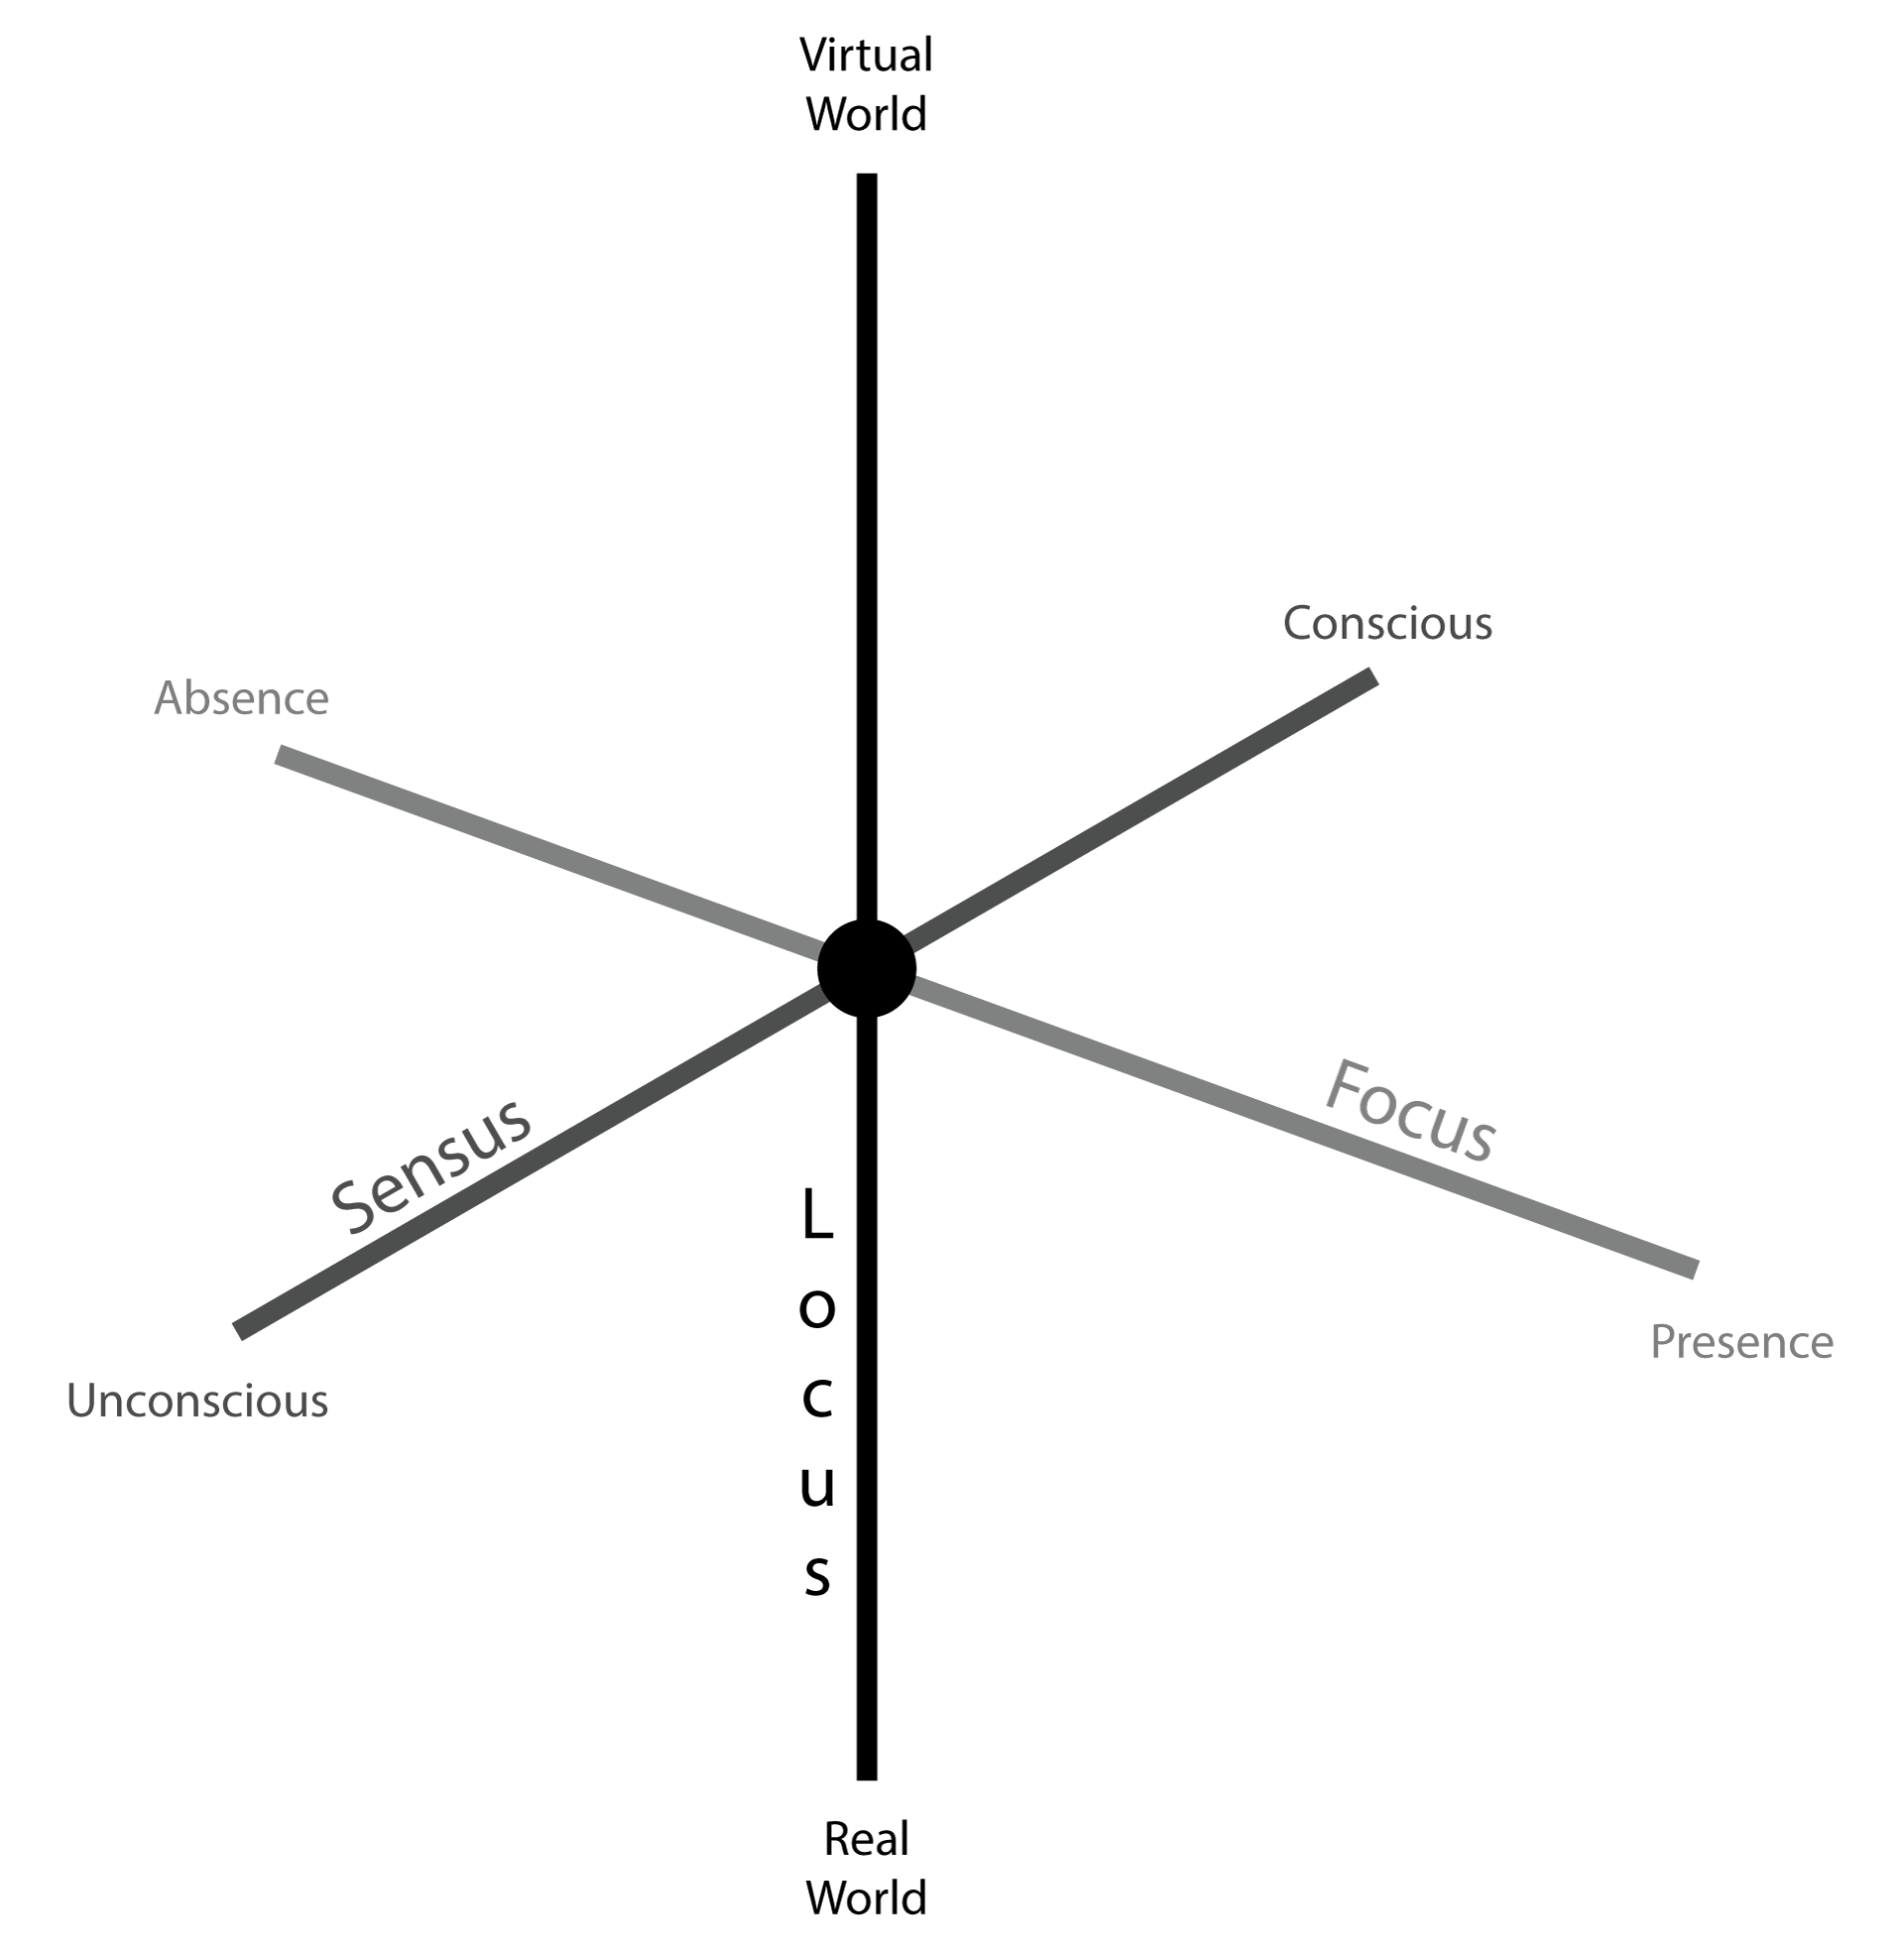
\includegraphics[width=.6\textwidth]{focus-locus-sensus-original.png}
		\caption{The three dimensions of virtual experience model.}
		\label{focus-locus-sensus-original}
	\end{center}	
\end{figure}

In the three dimensions of virtual experience model the \textit{locus of attention} axis represents the environment where the stimuli that the user is perceiving originate from; the \textit{focus of attention} axis represents the balance between conceptual/abstract reasoning and perceptual/concrete processing, where complex conceptual reasoning (or `distraction' from percepts~\cite{Chalmers2014}) results in little attention being paid to processing environmental percepts (whether originating from real stimuli, virtual stimuli, or a mix) thus reducing presence\presencefootnote{} in that environment toward its antithesis $-$ absence\absencefootnote{}; and the \textit{sensus of attention} axis represents the level of conscious arousal (or `wakefulness'~\cite{Laureys2009}) of the user, whether directed toward percepts originating from real stimuli, virtual stimuli, a mix of both, or not directed toward any percepts in the case of completely `absent' conceptual reasoning, a concept clarified by the authors:

\begin{quote}
	\textit{``Presence arises from active awareness of our embodiment in a present world around us. Presence is not consciousness, and we may be highly conscious while feeling absent, at those times when we are relatively unaware of our own embodiment.''}~\cite{Waterworth2014}
\end{quote}

In this model, the notion of involvement relates closely to the focus of attention axis; heightened involvement pertains to concentrating on environmental stimuli or meaningfully related activities and events, while heightened focus pertains to increased perceptual/concrete processing; lessened involvement pertains to a preoccupation with personal problems or activities occurring outwith the environment of interest, while lessened focus pertains to increased conceptual/abstract reasoning.

%=========================================================================================================

\subsection{The Combined Milgram/Waterworth Model}
\label{combined-milgram-waterworth-model}
With the locus of attention axis representing the environment from which the stimuli the user is perceiving originate from, a relationship can be drawn between the Waterworth model and Milgram and Kishino's reality-virtuality continuum, with the latter considered here to be analogous to the locus of attention axis. The combination of these two models in this manner gives rise to the combined Milgram/Waterworth model which is shown by figure \ref{focus-locus-sensus-with-virtuality-continuum} and allows for a novel method of visualising the experience of using alternate reality systems, including those that implement parallel reality.

\begin{figure}[h]
	\begin{center}
		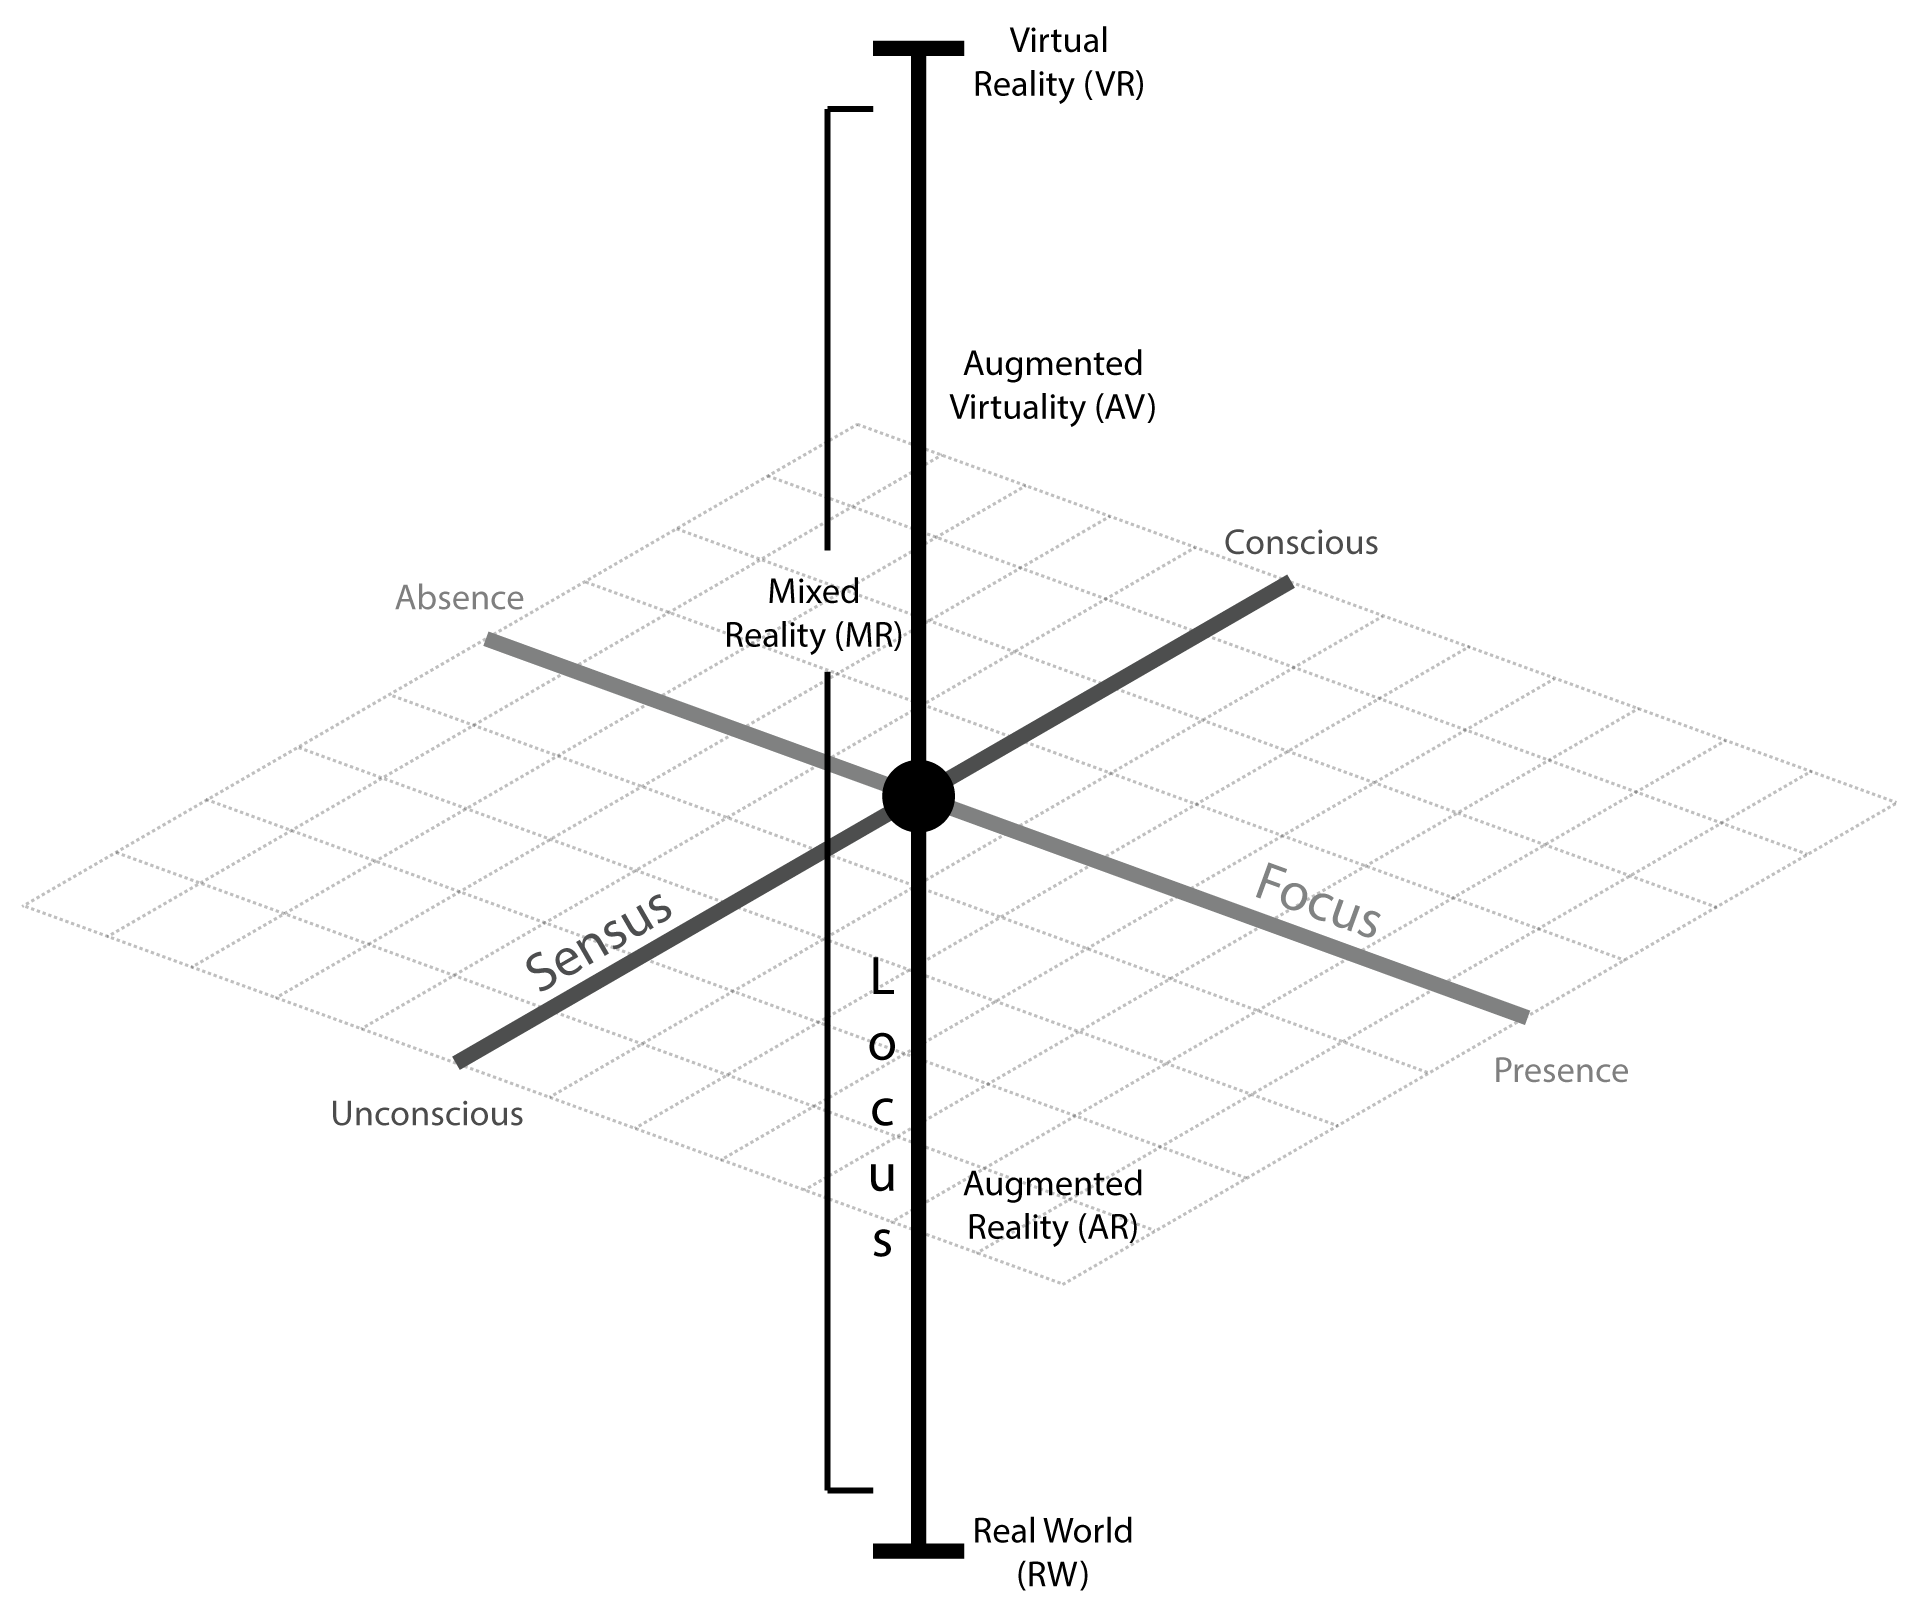
\includegraphics[width=.8\textwidth]{focus-locus-sensus-with-virtuality-continuum-updated-with-grid.png}
		\caption{The combined Milgram/Waterworth model.}
		\label{focus-locus-sensus-with-virtuality-continuum}
	\end{center}	
\end{figure}

Studying the combined Milgram/Waterworth model shows more clearly that the balance between presence and absence can relate to any environment upon the locus of attention axis, as confirmed by Waterworth and Waterworth:

\begin{quote}
	\textit{``We may feel hardly present at all in the physical world (a state we call absence) if nothing is happening there that is of interest or that impacts on our well-being, and so it is with mediated presence.''}~\cite{Waterworth2014}
\end{quote}

Furthermore one can postulate as to the essence of Lifton's vacancy with regard to the combined Milgram/Waterworth model (and thus to the experience of presence in general). Lifton's original definition presents vacancy as the `absence' of a person from one world while they are participating in the other, however the use of this term in Lifton's context differs to its use in the combined Milgram/Waterworth model. Lifton's absence refers to the inability to simultaneously perceive environmental stimuli from \textit{``more than one place (reality)''} while the absence of the combined Milgram/Waterworth model refers to increased conceptual/abstract reasoning resulting in a reduction of perceptual/concrete processing of all environmental stimuli. In terms of the combined Milgram/Waterworth model, the vacancy problem should be thought of as referring to the largely singular nature of a user's position upon the locus of attention axis.

%and the ability of a parallel reality platform toward reducing the problem, by allowing a user to `participate' in two environments at once, can be visualised either as extending the occupiable position upon the locus of attention axis from a singular position to a pair of positions (or as a range between two positions), or as reducing the deflection experienced upon the focus of attention axis from presence toward absence when performing a transition between two positions upon the locus of attention axis.

%The Sensus Dimension - the importance of being awake in class
%"Even as we sleep dreamlessly..." (example of being 'unconscious' in this regard)

%fourth axis is alterity, between hermeneutics and embodiment

%=========================================================================================================

\subsection{Experience in Parallel Reality}

\label{transitions_in_parallel_reality}

In terms of the combined Milgram/Waterworth model, the novel aspect of parallel reality can be visualised as the ability it imparts upon its user to freely switch their locus of attention between equivalent vantage points in real and virtual environments. In order to achieve the highest quality of experience with this style of interaction it is vital to determine how best to implement these transitions; that is, to mitigate the increased cognitive load (manifesting as increased conceptual reasoning and reduced perceptual processing) required to comprehend each transition, as this will detract from engagement with the environments and reduce the user's willingness to perform subsequent transitions. The ability of a parallel reality platform to mitigate the vacancy problem can be viewed as how well it reduces the deflection experienced upon the focus of attention axis from presence toward absence when performing a transition between two positions upon the locus of attention axis.

%In the systems developed by this thesis the users maintain mobility, such that they can move around the two environments in tandem, thus extending existing XR platforms that featured static locations at which a user in the real environment could see into the virtual and vice-versa. This combination of unhindered mobility with the ability to transition between real and virtual stimuli thus alleviates the vacancy problem.

%This is achieved by the user performing transitions between RW visual stimuli and VR visual stimuli, both presented via their HMD. This extends existing XR research by allowing the user to engage with the visual stimuli of the VR component of a XR system from any position and at any time.

Some researchers support the notion that in systems where more than one environment competes for the user's locus of attention there is an `all or nothing' Gestalt switch between awareness of one environment and the other~\cite{Slater2002}. Considering a parallel reality system, this notion would expect a substantial increase in cognitive load upon each transition between real and virtual environments. However the position adopted by this thesis is of the contrary opinion; that switching locus of attention from the stimuli of one environment to those of another does not completely overrule the user's awareness of the former. Instead, both environments can be perceived at the same time (albeit one to a lesser extent)~\cite{Ijsselsteijn2001} and when engaging with virtual content a user's focus can even be said to typically be \textit{shared} between the real and the virtual environments~\cite{Waterworth2001}, leading to a notion of `distributed' presence, or simultaneously experiencing a sense of presence in multiple environments.

This latter position is particularly apt for situations wherein the real and virtual environments share the same fundamental layout and dimensions (spatial equivalence), as those of the parallel reality systems explored within this thesis do, as inherent familiarity between two environments intuitively reduces the cognitive load associated with transitioning between them.

Furthermore, the notion of experience of presence as changing continually from moment-to-moment~\cite{Heeter2003, Ijsselsteijn1998} lends confidence to the successful mitigation of the increased cognitive load associated with these transitions to manageable levels. One might even liken this `switching' between real and virtual to the `cycling through' behaviour observed in users of virtual communities, which stemmed from the `window' concept of modern computer operating systems~\cite{Turkle2004} and accelerated with mobile devices to the point where for many users today rapid cycling stabilizes them into a sense of `continual copresence', where even just a mobile phone brings them into a world of continual partial attention to any particular subject or environment~\cite{Turkle2011}. The advent of mobile phones has previously been credited with allowing a person to \textit{``be in many places at once''} and to play multiple roles~\cite{Terashima2001}. The term polysocial reality was introduced to describe situations like this, of multiplexing physical reality with Web-based social networks and apps for Internet mediated social interaction~\cite{Applin2012}. As it has been shown that \textit{``effective interaction among participants is a contributing factor to presence''}~\cite{Terashima2001}, the importance of social interaction upon presence should not be understated.

%HyperReality p148

%=========================================================================================================

\subsection{Breaks in Presence}

\label{background-breaks-in-presence}

No matter how smooth the transition between real and virtual, the process is expected to nonetheless result in some heightened cognitive load, a temporary `break in presence' (BIP), as the user comes to terms with the new environment presented to them and comprehends its relation to the other environment that they were just perceiving. The definition of break in presence adopted herein is that introduced by Waterworth and Waterworth for the purposes of their three dimensions of virtual experience model~\cite{Waterworth2001}. Here, a break in presence represents a movement along the focus of attention axis away from presence in either a real, a virtual, or a mixed reality environment and toward absence. This differs to Slater and Steed's earlier usage of the term~\cite{Slater2000} wherein they considered presence in terms of `virtual presence', where a break in presence is a Gestalt switch from a sense of presence in a virtual environment to a sense of presence in the real environment.

\begin{quote}
	\textit{``When in a virtual environment, presence is typically shared between the VR and the physical world. `Breaks in presence' are actually shifts of presence away from the VR and toward the external environment. But we can also have `breaks in presence' when attention moves toward absence - when an observer is not attending to stimuli present in the virtual environment, nor to stimuli present in the surrounding physical environment''}~\cite{Waterworth2001}
\end{quote}

The Waterworth model considers presence in terms of attending to stimuli from either a real environment, a virtual environment, a mixed reality environment, or even multiple environments, with a break in presence representing absence in the sense of heightened conceptual load and the resultant reduced perceptual processing of environmental stimuli, no matter the provenance of those stimuli. This usage better fits the situations invoked by the parallel reality concept, which is concerned with intentionally and willingly switching engagement between stimuli from both real and virtual environments, rather than engaging with stimuli from only a virtual environment in a scenario wherein stimuli from the real environment are considered a `distraction'.

This difference between the Steed and Waterworth uses of break in presence can be visualised by considering the axes of the combined Milgram/Waterworth model. In the Steed definition a break in presence represents a movement upon the locus of attention axis from the virtual world to the real world. In the Waterworth definition a break in presence represents a movement upon the focus of attention axis from presence to absence, regardless of position upon the locus of attention axis.

Transitions between the virtual world and the real world can be implemented in multiple different manners and it is expected that users may prefer different implementations in different situations, surroundings and scenarios. Preference toward a particular implementation is posited to correlate with a less severe break in presence being experienced upon its execution. This thesis explores several different transition implementations, both in order to identify and quantify preferences toward them in general, and to infer any relationships between transition preference and particular situational states.

%=========================================================================================================

\subsection{Parallel Reality and the Combined Milgram/Waterworth Model}
Visualised using the combined Milgram/Waterworth model, the transitions of a parallel reality system are an oscillation between two different positions upon the locus of attention axis. Figure \ref{focus-locus-sensus-with-virtuality-continuum-with-transition} shows an example where a user performs a smooth transition between perceiving stimuli from a fully real environment and a fully virtual environment.

Heightened cognitive load required to comprehend the transition is represented by a temporary movement upon the focus of attention axis from presence toward absence (a break in presence). With the ability of a wide field of view (FOV), stereoscopic 3D, head-tracked HMD (such as that used by the Mirrorshades platform developed in this thesis) to produce immersive virtual reality visual stimuli that require fairly limited cognitive processing and our inherent ability to engage with our real surroundings without significant cognitive load, focus is represented as being high (toward the presence extreme) when attending to stimuli from either the real or virtual environments.

Sensus is expected to be largely task dependent, however when performing a task that involves actively engaging with the visual stimuli from either/both of the real and virtual environments it is expected to be high (toward the conscious extreme). Upon triggering a transition, sensus is expected to increase, as the user centres their attention upon relating the visual stimuli from the new environment to those they were just perceiving from the other environment

%Whilst continued exposure to the platform is expected to reduce the severity of the BIPs, mitigating their severity from the outset (reducing the displacement from the presence extremum downwards toward absence) through informed execution of the transitions between RW and VR is believed to be important to the overall quality of experience that users receive.

%absent-mindedness - caused by increased attention toward a single object of focus (hyperfocus, eg the object of focus is the switch)
% or caused by distraction (again, the switch)

\begin{figure}[h]
	\begin{center}
		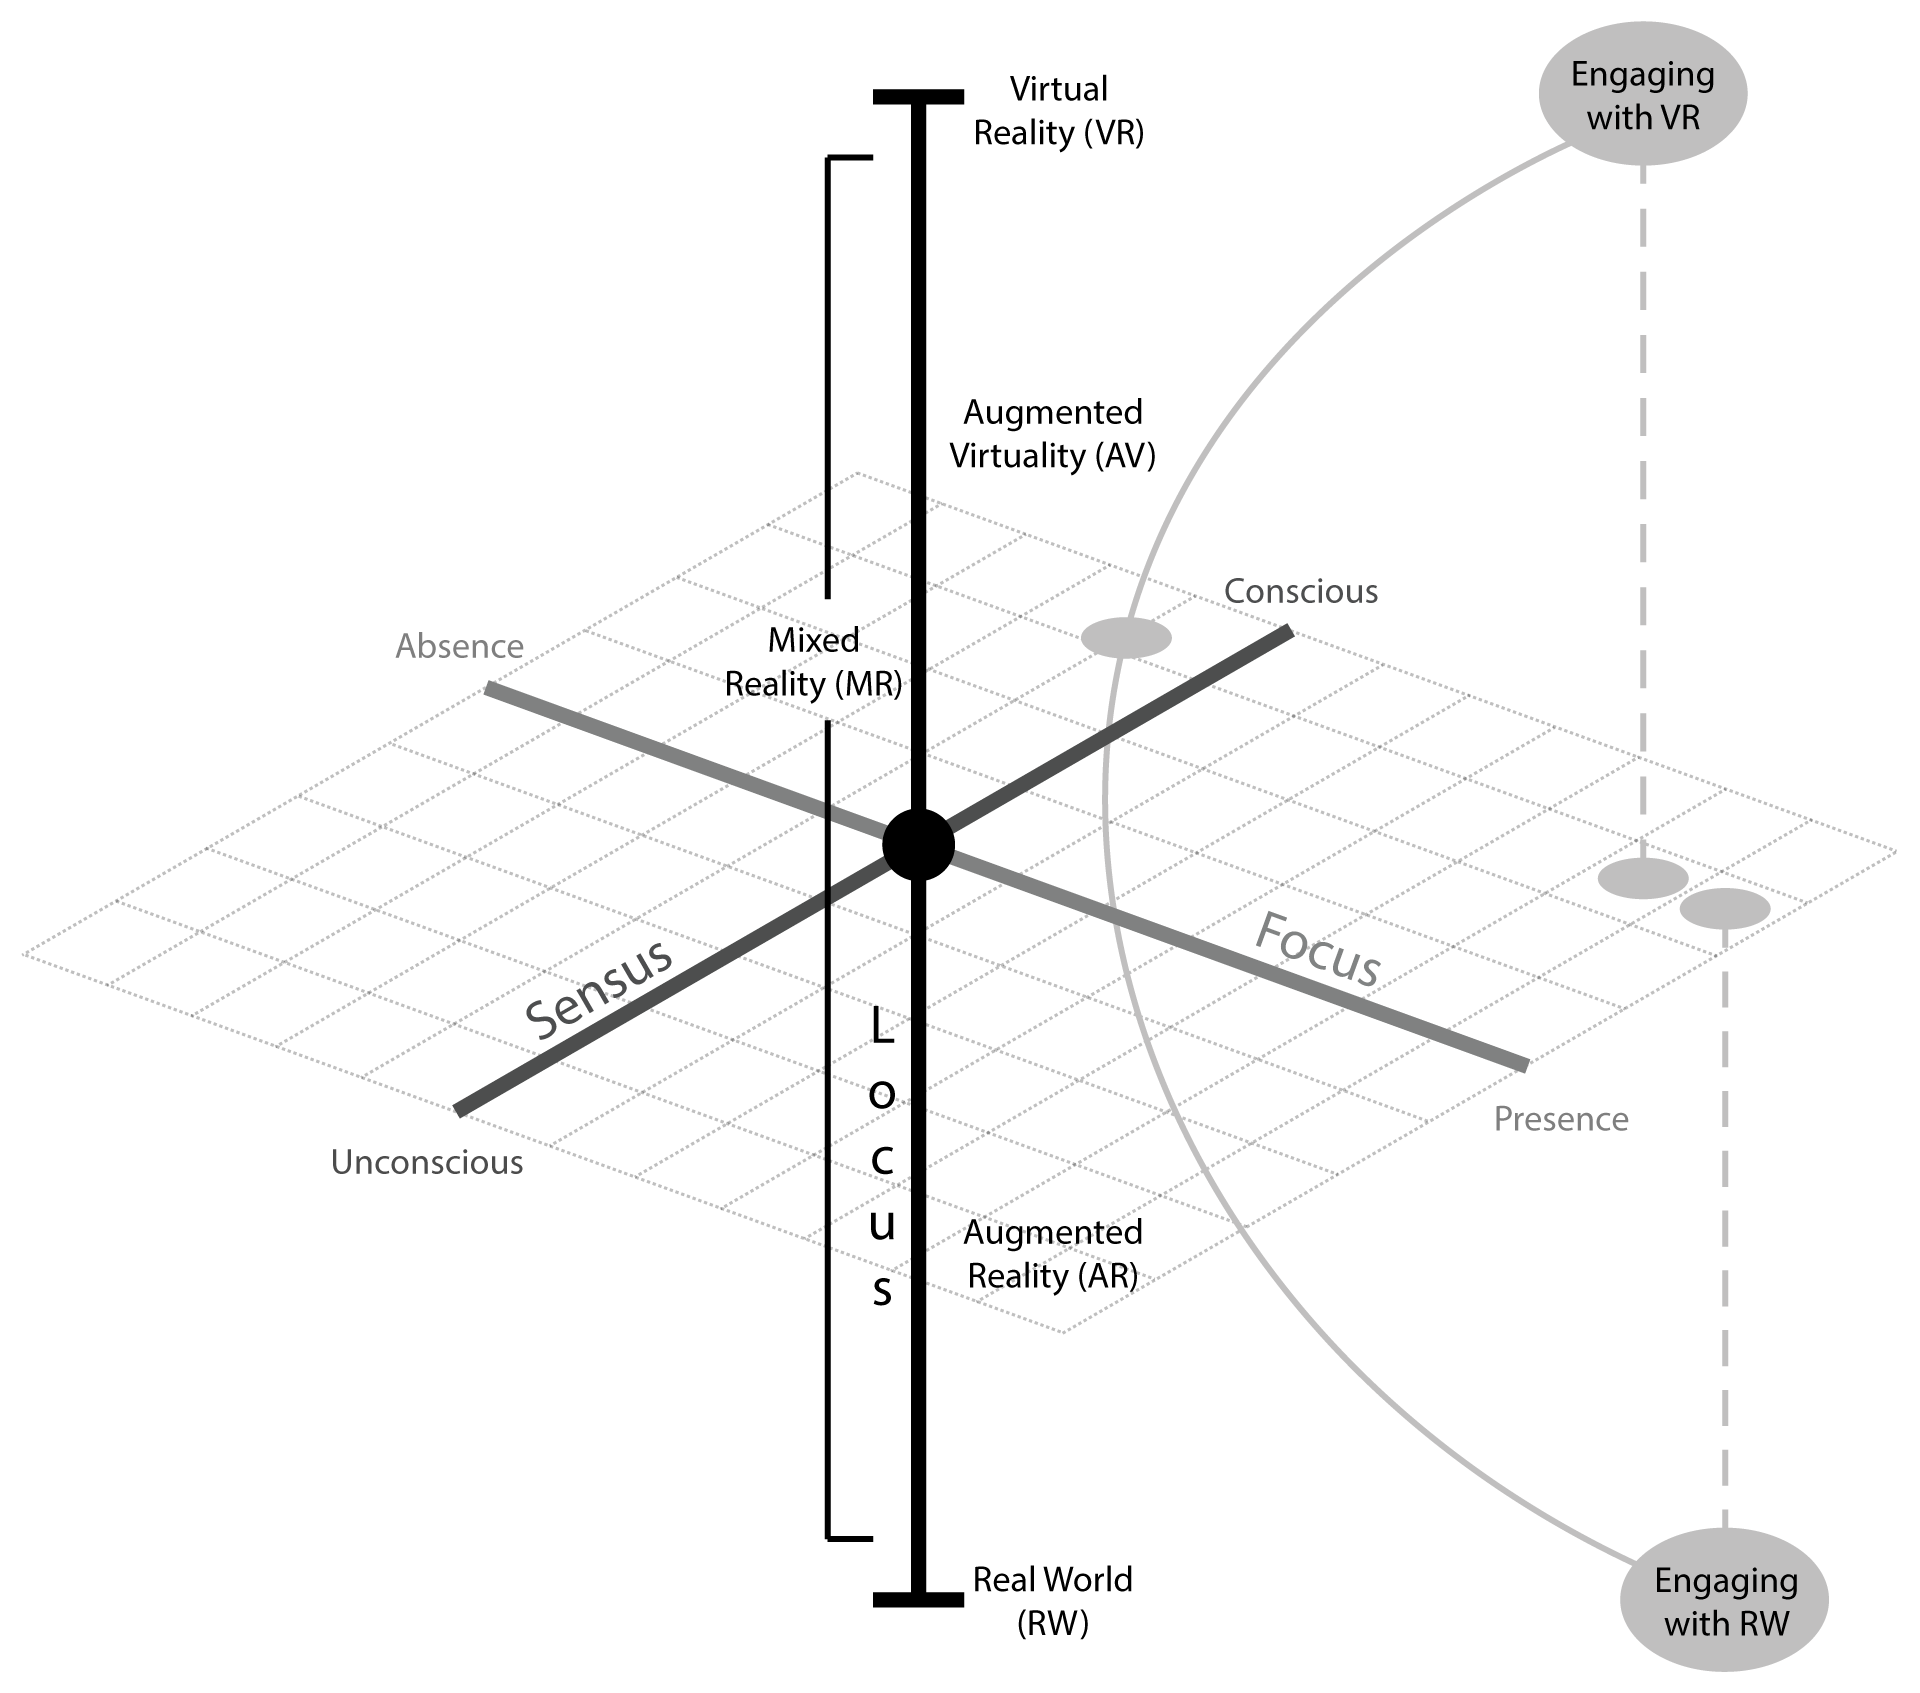
\includegraphics[width=.8\textwidth]{transition-rw-vr.png}
		\caption{Visualisation using the combined Milgram/Waterworth model of the theorised experience of a user of a HMD based parallel reality system performing a smooth transition between its constituent real and virtual environments.}
		\label{focus-locus-sensus-with-virtuality-continuum-with-transition}
	\end{center}	
\end{figure}

%=========================================================================================================
%=========================================================================================================


%=========================================================================================================
%=========================================================================================================
%=========================================================================================================
%=========================================================================================================
%=========================================================================================================
%=========================================================================================================
%=========================================================================================================
%=========================================================================================================
%=========================================================================================================
%=========================================================================================================


%Users are free to explore and interact with either environment in relative isolation from the other, even if their interactions in one trigger changes in the other, however simultaneous interaction and exploration with both environments has largely remained without systematic investigation.

%This is largely because users exploring and interacting with the real environment do not have a convenient manner of also exploring and directly interacting with the virtual environment, as such interaction usually relies upon the use of software run on a desktop or laptop computer which is not conducive to mobile use. Using a laptop computer whilst walking around is far from convenient and using a desktop computer obviously limits the user's interaction with the real environment to that immediately around the location of the  computer and results in a disjoint relationship between their physical position in the real environment and the location of their avatar in the virtual environment when they navigate their avatar away from the respective position of their computer. This situation has been called `the vacancy problem'; an apparent vacancy from one environment whilst engrossed in the other.




%=========================================================================================================
%=========================================================================================================





%=========================================================================================================

%Marie Kim et al at The Electronics and Telecommunications Research Institute, Korea, explain the cross reality paradigm well in terms of its principle features

%\begin{quote}
%\textit{``The important point of X-reality is a paradigm shift from single-directional information flows to bidirectional information flows between two worlds.''}
%\end{quote}

%and also how it can be employed for simultaneous presence in real and virtual environments

%\begin{quote}
%\textit{``The differential characteristic of X-reality is that it can augment user's engagement in the experiences of virtual presence and virtual world. Ultimately, it results in the human life span extension from the only real world to both worlds.''}
%\end{quote}





%Paradiso in IEEE Pervasive, Cross Reality Environments ~\cite{Paradiso2009} \textbf{***check this is the right citation***}

%\begin{quote}
%\textit{We call the ubiquitous mixed reality environment that comes from the fusion of these two technologies cross-reality. Sensor networks can tunnel dense real-world information into virtual worlds, where this data is interpreted and displayed to dispersed users. Interaction of virtual participants can incarnate into the physical world through a plenitude of diverse displays and actuators. We can envision a user's interface into this environment as an extension of human perception and interaction, augmenting our five senses well beyond the canonical ``here and now'' and redefining the meaning of presence.''}
%\end{quote}



%\begin{quote}
%\textit{``We see cross-reality precipitating when diverse and ubiquitous sensor and actuator networks meet pervasively shared online virtual worlds, where phenomena freely tunnel between real and contrived continua at a multitude of ``wormholes'' opened by densely deployed networked devices, seamlessly adapting the level of immersion to match a variable ecology of available interfaces and user context or preference.''}~\cite{Lifton2009}
%\end{quote}


%=========================================================================================================

\section{Summary}
Decades of research into alternate realities has furnished us with a rich continuum of approaches and technologies for creating, combining, augmenting and diminishing real and virtual environments. Many of the alternate reality labels that are now becoming commonplace are concerned with presenting a different environment to the user's real surroundings (as in telepresence and virtual reality) or mixing additional information into the user's view of their real or virtual surroundings (as in augmented reality and augmented virtuality).

Although less thoroughly investigated, the concept of creating an alternate reality system by combining two complete environments, one real and the other virtual, into a cross reality system presents an interesting avenue for furthering alternate reality techniques and applications, in particular to addressing the vacancy problem that affects users when trying to distribute their attention between two environments. Previous cross reality research has focussed upon alleviating this vacancy problem by integrating sensor and actuator infrastructure into the constituent real and virtual environments of a system, such that actions and events in one environment could manifest into the other. However direct visual engagement with both environments was not often possible in these systems and only from predetermined, static locations.

Parallel reality has been introduced as a new category of alternate reality that allows its user to visually engage with both a real and a virtual environment at any position, freely switching between them at any time. In trading the sensor/actuator infrastructure of a cross reality system for direct visual engagement with both environments, the parallel reality concept further addresses the vacancy problem by truly providing \textit{``the means to be in more than one place (reality) at a time''}\cite{Lifton2007a}.
%\begin{quote}
\textit{``Where are you?'' Hiro says.
\\
\\
``In Reality or the Metaverse?''
\\
\\
``Both.''}
\end{quote}
\hfill \textit{Snow Crash, Neal Stephenson}
\\
\\
\\

%=========================================================================================================
%=========================================================================================================

% 'Position' section from experimental plan document

%\section{Introduction}

The subject of this thesis is the design, development \& evaluation of platforms that allow their users to observe \& move around their real environment whilst also being able to view an alternative virtual environment from the equivalent vantage point. This combination of `parallel' real \& virtual environments, combined with maintained mobility, is not well encapsulated by any previously defined alternate reality terminology, thus it is necessary to explore this alternate reality terminology \& technologies in order to correctly frame these systems in relation to them.

The closest existing label is the \textit{cross reality} paradigm, as a cross reality system holds the distinction of two discrete environments, one real \& one virtual, complete-unto-themselves, however cross reality further focusses on a bidirectional exchange of information between the environments \& not upon user mobility \& tandem visual exploration of both environments.

Thus, we propose the new term \textit{parallel reality} to refer to systems that combine complete \& discrete real \& virtual environments together in a manner that allows mobile exploration of them both in tandem, relating it \& positioning it against existing alternate reality terminology previously explored by computer science \& other disciplines.

%This research centres around the design, development \& evaluation of a hardware \& software platform which allows its user to observe \& move around their Real World (RW) environment whilst wearing a wide field of view (FOV), stereoscopic 3D, Head Mounted Display (HMD) which allows them to alternatively view an immersive Virtual Reality (VR) environment from the equivalent vantage point. This is achieved by combining a head-tracked HMD, webcams, an indoor positioning system (IPS) \& a 3D game engine, into a mobile \textit{cross reality} (XR) interface.

%One of the distinguishing features of XR is that, by linking real \& virtual environments more closely, it mitigates the `vacancy problem': \textit{``the noticeable \& profound absence of a person from one world, either real or virtual, while they are participating in the other''}, which arises \textit{``because people do not currently have the means to be in more than one place (reality) at a time''}~\cite{Lifton2007a}.

%Previous XR research approached the vacancy problem by integrating sensor/actuator networks into the environments, such that actions in one could manifest in the other, however direct visual engagement with the virtual environment was only possible from static interfaces at pre-determined locations within the real environment~\cite{Lifton2007a, Dublon2011}. The platform discussed in this document addresses this shortcoming by providing a mobile interface for visual engagement with both environments of a XR system, allowing the user to transition between viewing their real environment \& a virtual environment at any time while maintaining the freedom to move around them, multiplexing visual stimuli from their real surroundings \& from a parallel, virtual `mirror world'~\cite{Gelernter1993}.

%=========================================================================================================
%=========================================================================================================

\section{Defining Alternate Realities}

Alternate realities have received substantial attention in recent decades, the themes explored for purposes as diverse as education~\cite{Warburton2009} \& new forms of data visualisation~\cite{Coleman2009} to medical~\cite{TenEyck2011} \& military training~\cite{Qiu2009}. Although terms such as \textit{mixed reality} \& \textit{augmented reality} are now relatively common in conversation \& literature, definitions of such terms have often been used in vague \& even conflicting manners.

This chapter will investigate popular definitions, classifications \& comparisons of alternate realities, combining \& modifying these parameters to produce a canonical set of definitions for the remainder of this thesis, explaining `parallel reality' into these definitions \& models.

\subsection{Milgram \& Kishino's Reality-Virtuality Continuum}

Paul Milgram, Herman Colquhon and Fumio Kishino addressed the issue of alternate reality definitions in detail and can be accredited with introducing the terms \textit{augmented virtuality} and \textit{mixed reality} to the literature, prompted by their identification of the need for more encompassing terms to supplement the existing definitions of \textit{augmented reality}~\cite{Milgram1994, Milgram1999}.

%However despite these thorough and well-reasoned definitions being published originally in 1994, much of the subsequent literature studied for this review has adopted conflicting, or at least confusing and misleading, definitions.

One of the overbearing concepts introduced by Milgram et al. is that whilst both purely real and purely virtual environments do exist they should not be considered discrete alternatives but rather poles lying at opposite ends of a linear scale $-$ the \textit{Reality-Virtuality continuum}. The location of an environment along this continuum coincides with its location along a parallel \textit{Extent of World Knowledge continuum} where `world knowledge' refers to the amount of quantitative information that is associated with the content being presented, or in other words how much of the environment is being `modelled' by a computer. These continua are included as figure \ref{reality_virtuality_extent_of_world_knowledge_continuum}.

\begin{figure}[h]
\centering
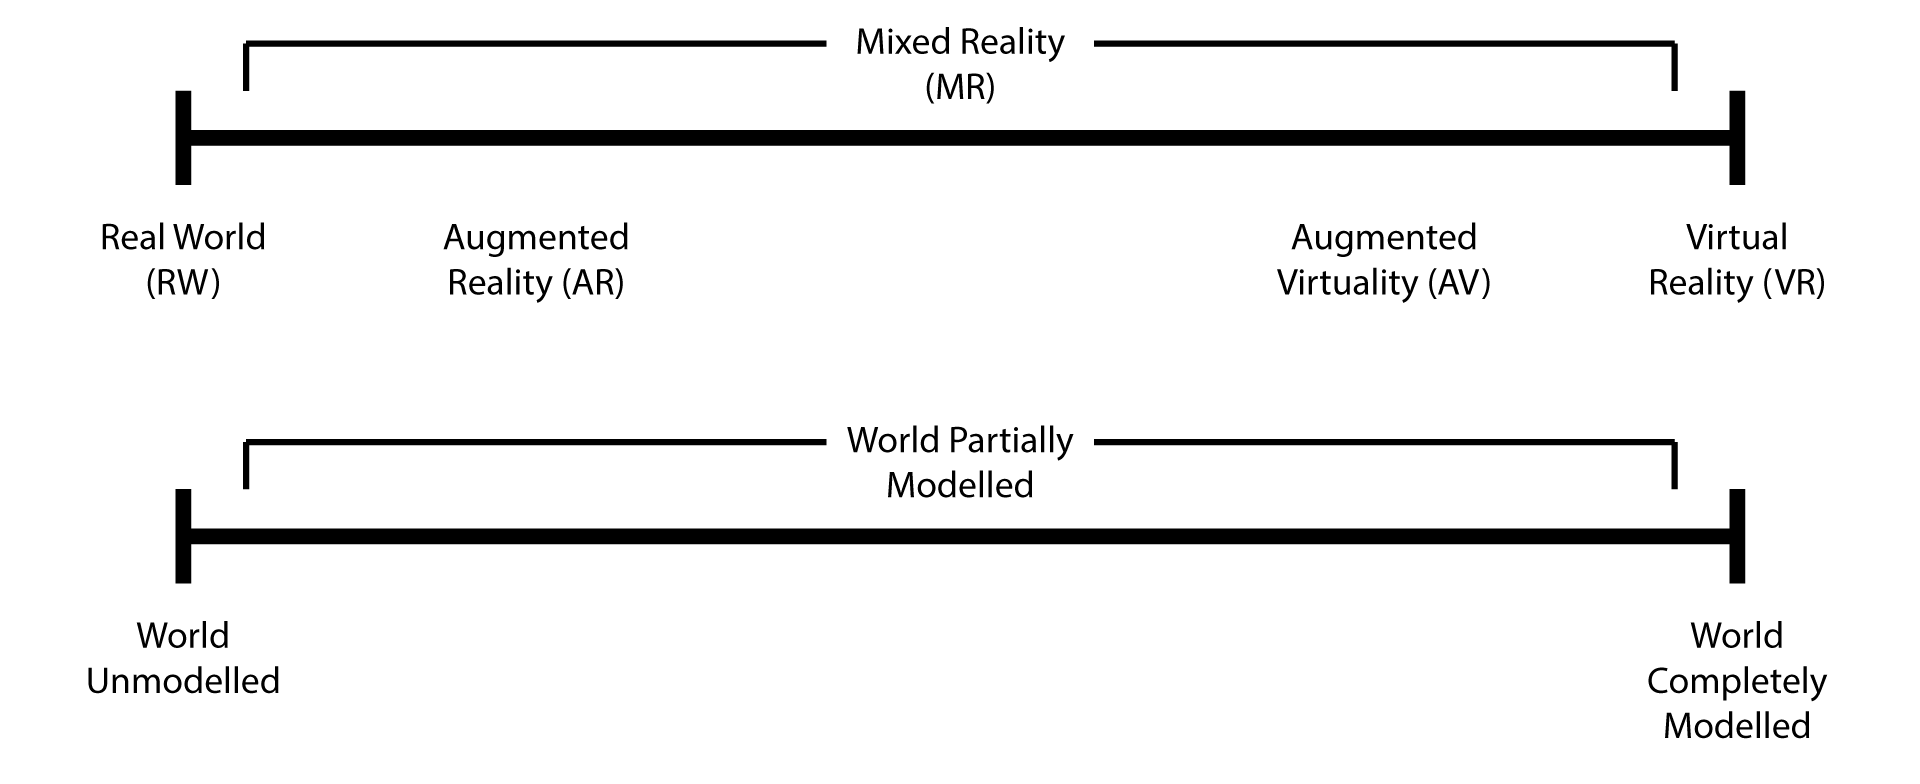
\includegraphics[width=\textwidth]{virtuality_continuum_extent_of_world_knowledge_continuum.png}
\caption{\textit{Reality-Virtuality continuum} (top), parallel with \textit{Extent of World Knowledge continuum} (bottom).}
\label{reality_virtuality_extent_of_world_knowledge_continuum}
\end{figure}

With a purely virtual environment, the entire viewport must necessarily be computer modelled in order to be rendered and as such there is complete quantitative information about all objects and between all objects being presented. At the opposite end of the spectrum with a completely real environment where none of the viewport is computer modelled there is no quantitative information associated with the content being displayed. At any point between the extremes the environment consists of a mixture of some modelled and some non-modelled content; with the computer associating quantitative information to, and between, the virtual objects, but not to the real objects or between the virtual and real objects.

Carrying the continuum concept further, Milgram et al. illustrate their understanding of the existing term \textit{augmented reality} and also introduce two related new terms; \textit{augmented virtuality} and \textit{mixed reality}. In this fashion, \textit{mixed reality} is used to describe any environment that is not completely real or completely virtual; that is, it encompasses all positions on the continuum between the extremes. \textit{Augmented reality} is used to describe a real environment upon which virtual objects are overlain and \textit{augmented virtuality} is used to describe a virtual environment upon which objects sampled from the real world (such as video feeds) are overlain. It is also shown here that \textit{mixed reality} encompasses both \textit{augmented reality} and \textit{augmented virtuality}.

One obvious question raised from studying this figure is at what point toward the centre of the continuum an environment changes from being \textit{augmented reality} into \textit{augmented virtuality} or vice-versa. The answer lies with consideration of the quantitative knowledge associated with the objects that comprise the viewport.

For example, if one were to take a viewport depicting a purely real environment and then incrementally add more and more virtual objects, the environment's classification would progress rightward along the continuum. Eventually the entire viewport would be obscured by virtual objects and the obvious conclusion would be to classify the environment as being purely virtual. However this would only be true if there was complete quantitative information associated with, and between, all of the virtual objects within the real 3D space of the viewport, which is unlikely to be the case.

Likewise if one were to take a viewport depicting a purely virtual environment and incrementally replace the entire viewport with sampled real objects we could not classify the resultant environment as purely real as there would be associated quantitative knowledge with and between the sampled objects, meaning that the environment isn't completely unmodelled and thus can't be classified as purely real.

Thus, Milgram et al. conclude, it is not necessarily true that an environment is purely virtual simply because all of the visible objects are computer modelled, nor is it necessarily true that an environment is purely real simply because all of the visible objects are sampled from the real world.

%=========================================================================================================

\subsection{Roy Want's Virtuality Matrix}

Another method of illustrating the relationships between different categories of alternate realities was put forward by Roy Want in his introductory article for a 2009 issue of IEEE Pervasive Computing dedicated to the \textit{cross reality} paradigm~\cite{Want2009}. He presents a 2x2 matrix categorising the different terms according to whether the experience and overlay data are real or virtual (figure \ref{original_virtuality_matrix.png}). Whilst this is a useful representation, some of the definitions \& criteria depicted do not match with those of Milgram et al. or even with those of other authors in the same issue of Pervasive, let alone other publications concerning alternate realities. Figure \ref{modified_virtuality_matrix.png} presents a modified version of this matrix that is in keeping with the framework laid out by Milgram et al. \& the wider literature.

\begin{figure}[h]
\centering
\begin{minipage}{.5\textwidth}
 	\centering
 	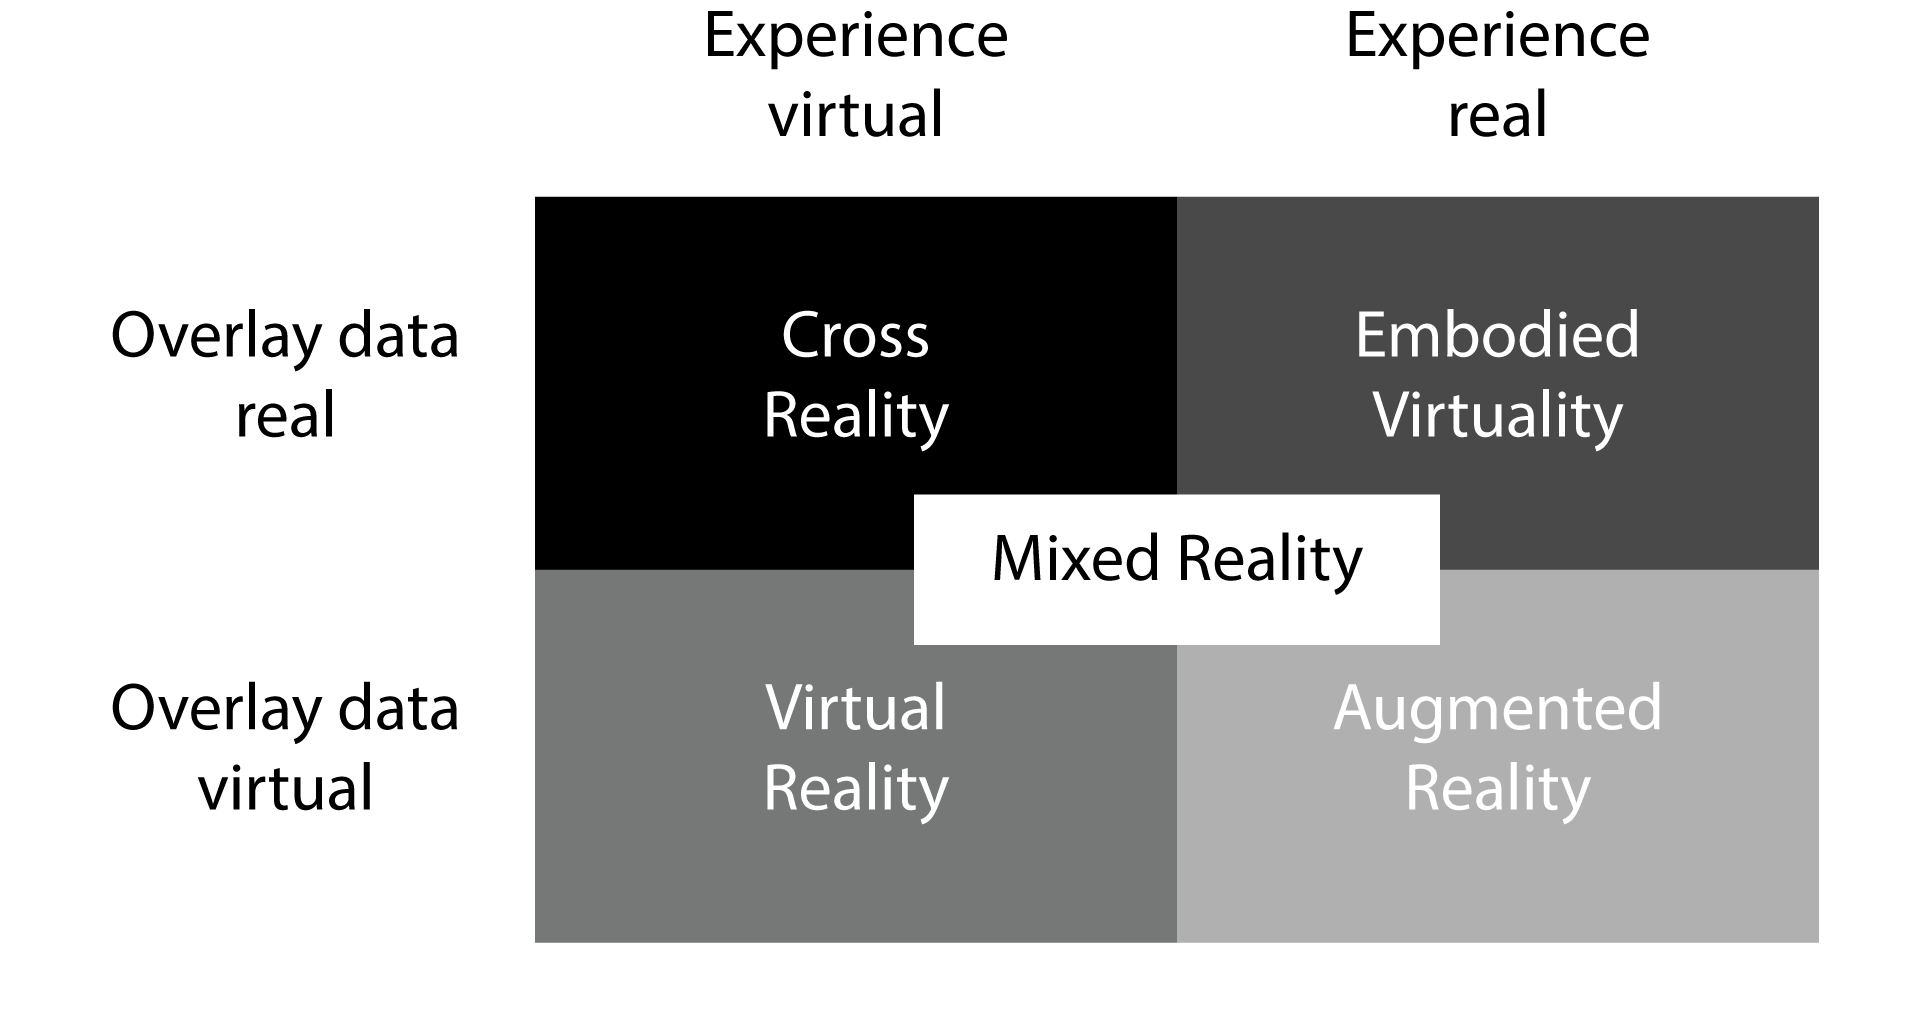
\includegraphics[width=0.95\linewidth]{Want_virtuality_matrix_original.png}
 	\caption{Want's original virtuality matrix.}
	\label{original_virtuality_matrix.png}
\end{minipage}%
\begin{minipage}{.5\textwidth}
  \centering
  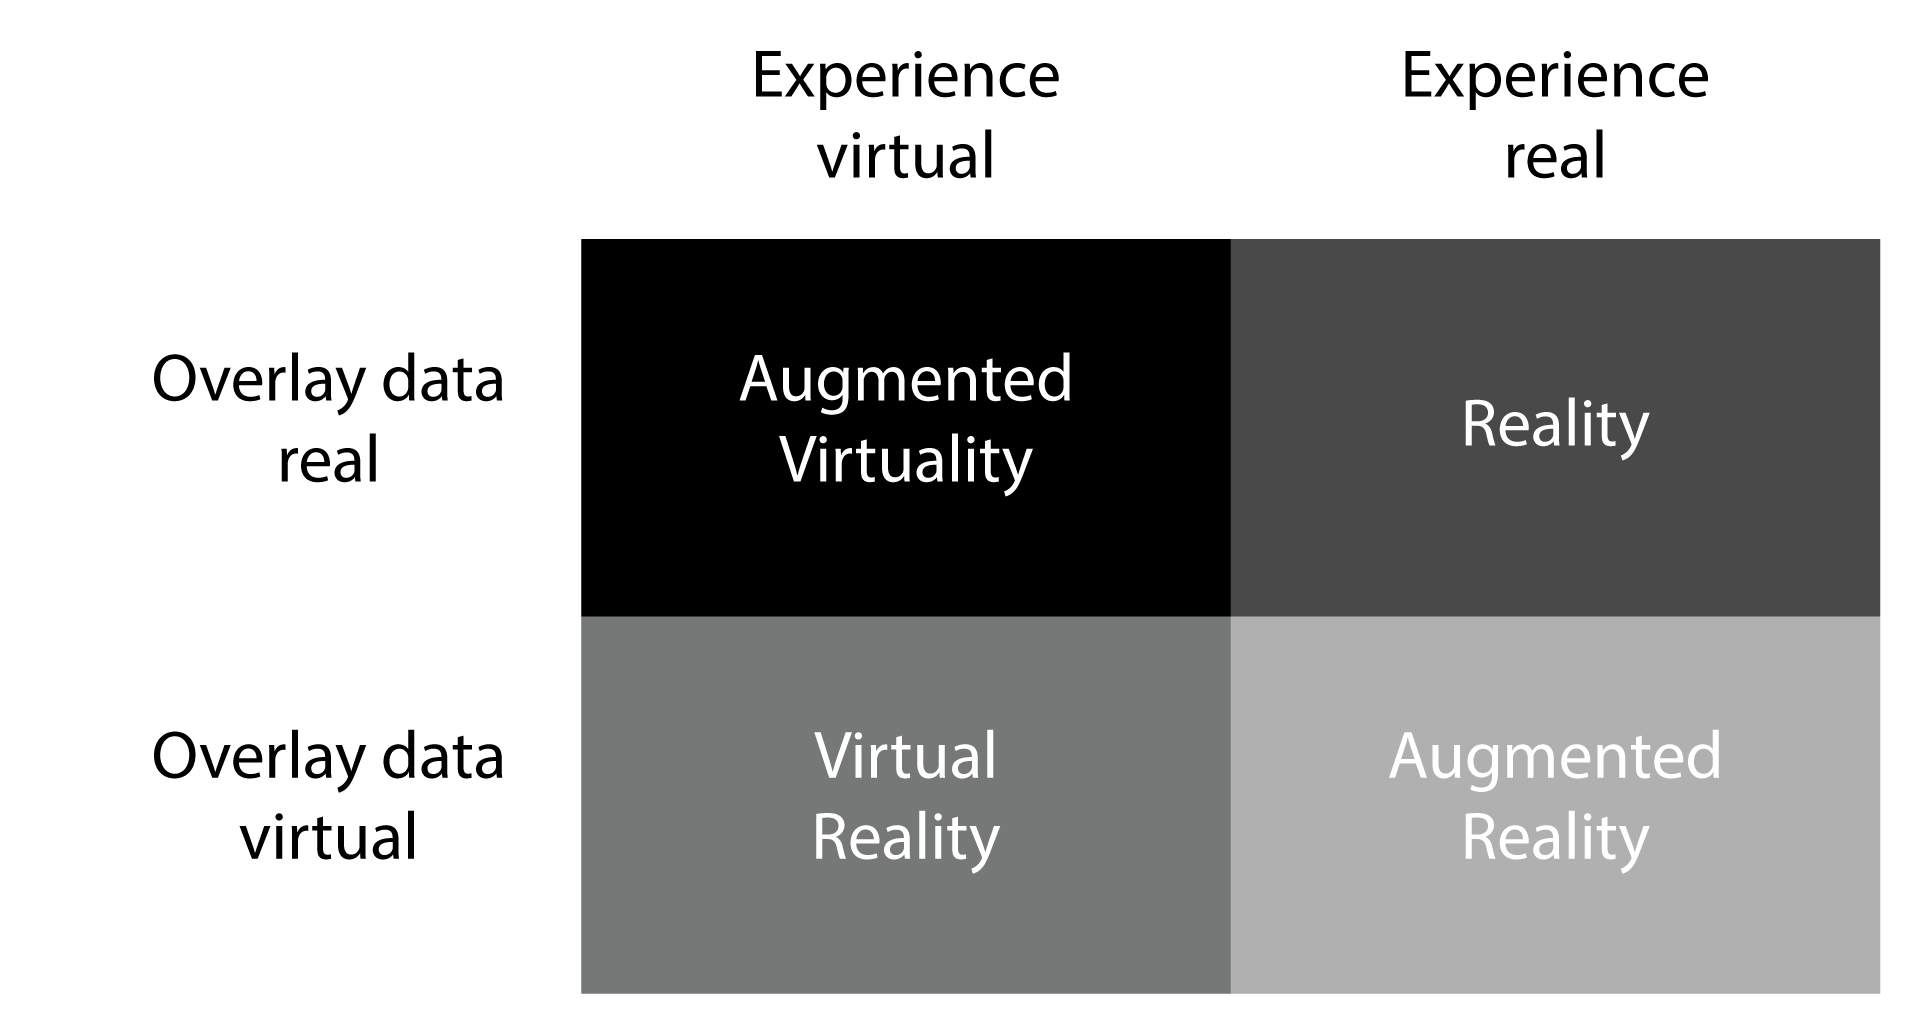
\includegraphics[width=0.95\linewidth]{Want_virtuality_matrix_modified.png}
    \caption{Modified Want matrix.}
    \label{modified_virtuality_matrix.png}
\end{minipage}
\end{figure}

Where the original matrix positions \textit{cross reality} in the upper left quadrant, at the congruence of `experience virtual' and `overlay data real', the modified matrix positions \textit{augmented virtuality}. Referencing Milgram's continuum, `experience virtual' relates to a position somewhere within the right half, while `overlay data real' relates to presentation over this necessarily virtual environment of sampled real world data, resulting in a partially modelled environment, leaving us in the area of the continuum occupied by \textit{augmented virtuality}.

The original matrix also features the term \textit{embodied virtuality} in the upper right quadrant, at the congruence of `experience real world' and `overlay data real'. Want explains that this is an alternative term for \textit{ubiquitous computing} which is \textit{``essentially the opposite of VR''}. The modified matrix adopts the position that the opposite of \textit{virtual reality} is simply \textit{reality} and that \textit{ubiquitous computing} does not constitute an alternate reality but rather a different model of human-computer interaction (that can be implemented in either \textit{reality} or \textit{augmented reality}, depending upon how the computing infrastructure presents information to users). A \textit{ubiquitous computing} system is necessarily a real environment, as it is by definition the integration and dissemination of computational infrastructure into our real surrounds~\cite{York2004}. However whether this real environment is augmented by virtual objects is not restricted by the concept.

Finally the modified matrix removes the central \textit{mixed reality} section from the original matrix, as its position is misleading. As the boundaries formed between the categories by the different colours could be construed as meaning that there are discrete boundaries between the different categories, the reader could be led to believe that a purely \textit{virtual reality} or a purely \textit{embodied virtuality} environment can be considered \textit{mixed reality}, which is incorrect. If one wished to picture the position of \textit{mixed reality} in relation to the modified matrix, it would cover the same area as enclosed by the union of \textit{augmented virtuality} and \textit{augmented reality}.

%=========================================================================================================

\subsection{Steve Mann's Venn Diagrams}

Steve Mann, a veteran of wearable computing \& one of the original MIT `gargoyles' etc. \textbf{***insert stuff here about him***}. used Venn diagrams to illustrate the relationships between the different categories of alternate realities (figure \ref{Mann_venn_original.png}).

Mann introduces the terms \textit{modulated reality} \& \textit{mediated reality} \textbf{***need the paper to read***}.

Mann's original diagram places augmented reality at a subset of mixed reality, but then further places virtual reality at a subset of augmented reality \& in turn mixed reality. A modified version of this diagram (figure \ref{Mann_venn_mod_1.png}) removes virtual reality from this position, introduces augmented virtuality \& positions both augmented reality \& augmented virtuality such that they overlap with modulated reality (as it is perfectly feasible for a modulated reality system to feature real or virtual augmentations).

\begin{figure}[h]
\centering
\begin{minipage}{.5\textwidth}
  \centering
  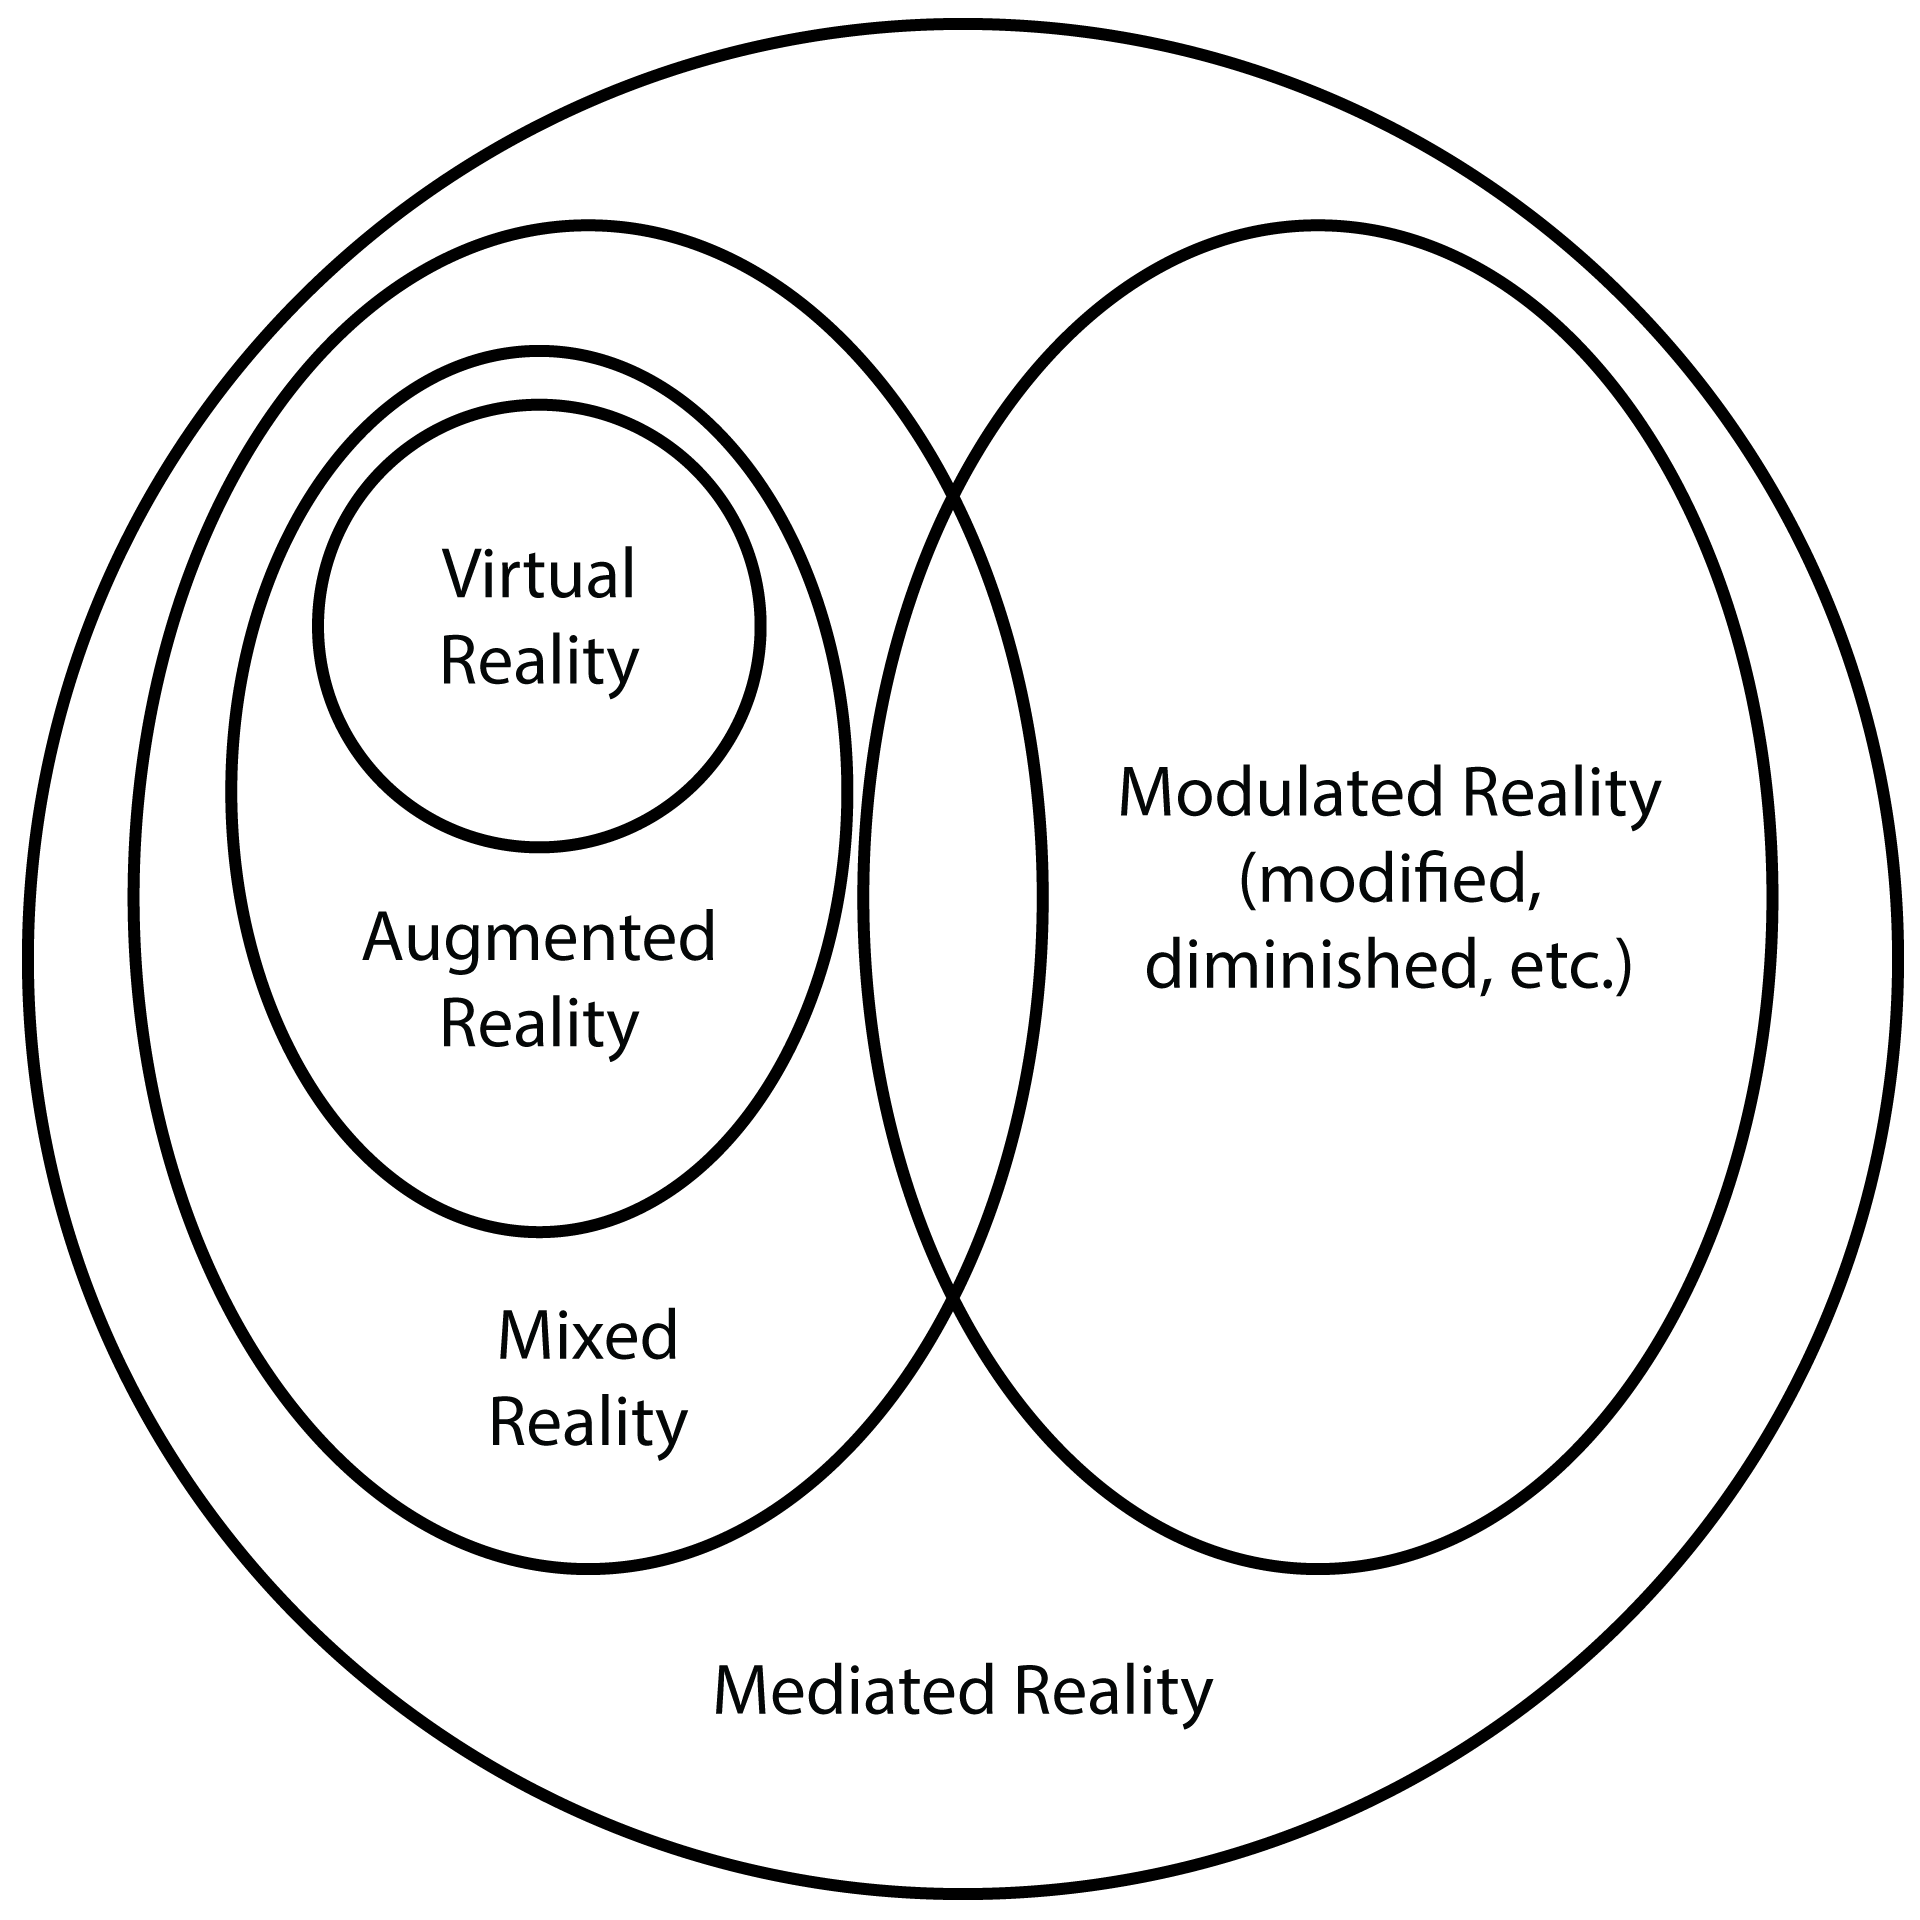
\includegraphics[width=0.95\linewidth]{Mann_venn_original.png}
  \caption{Original Mann venn diagram.}
  \label{Mann_venn_original.png}
\end{minipage}%
\begin{minipage}{.5\textwidth}
  \centering
  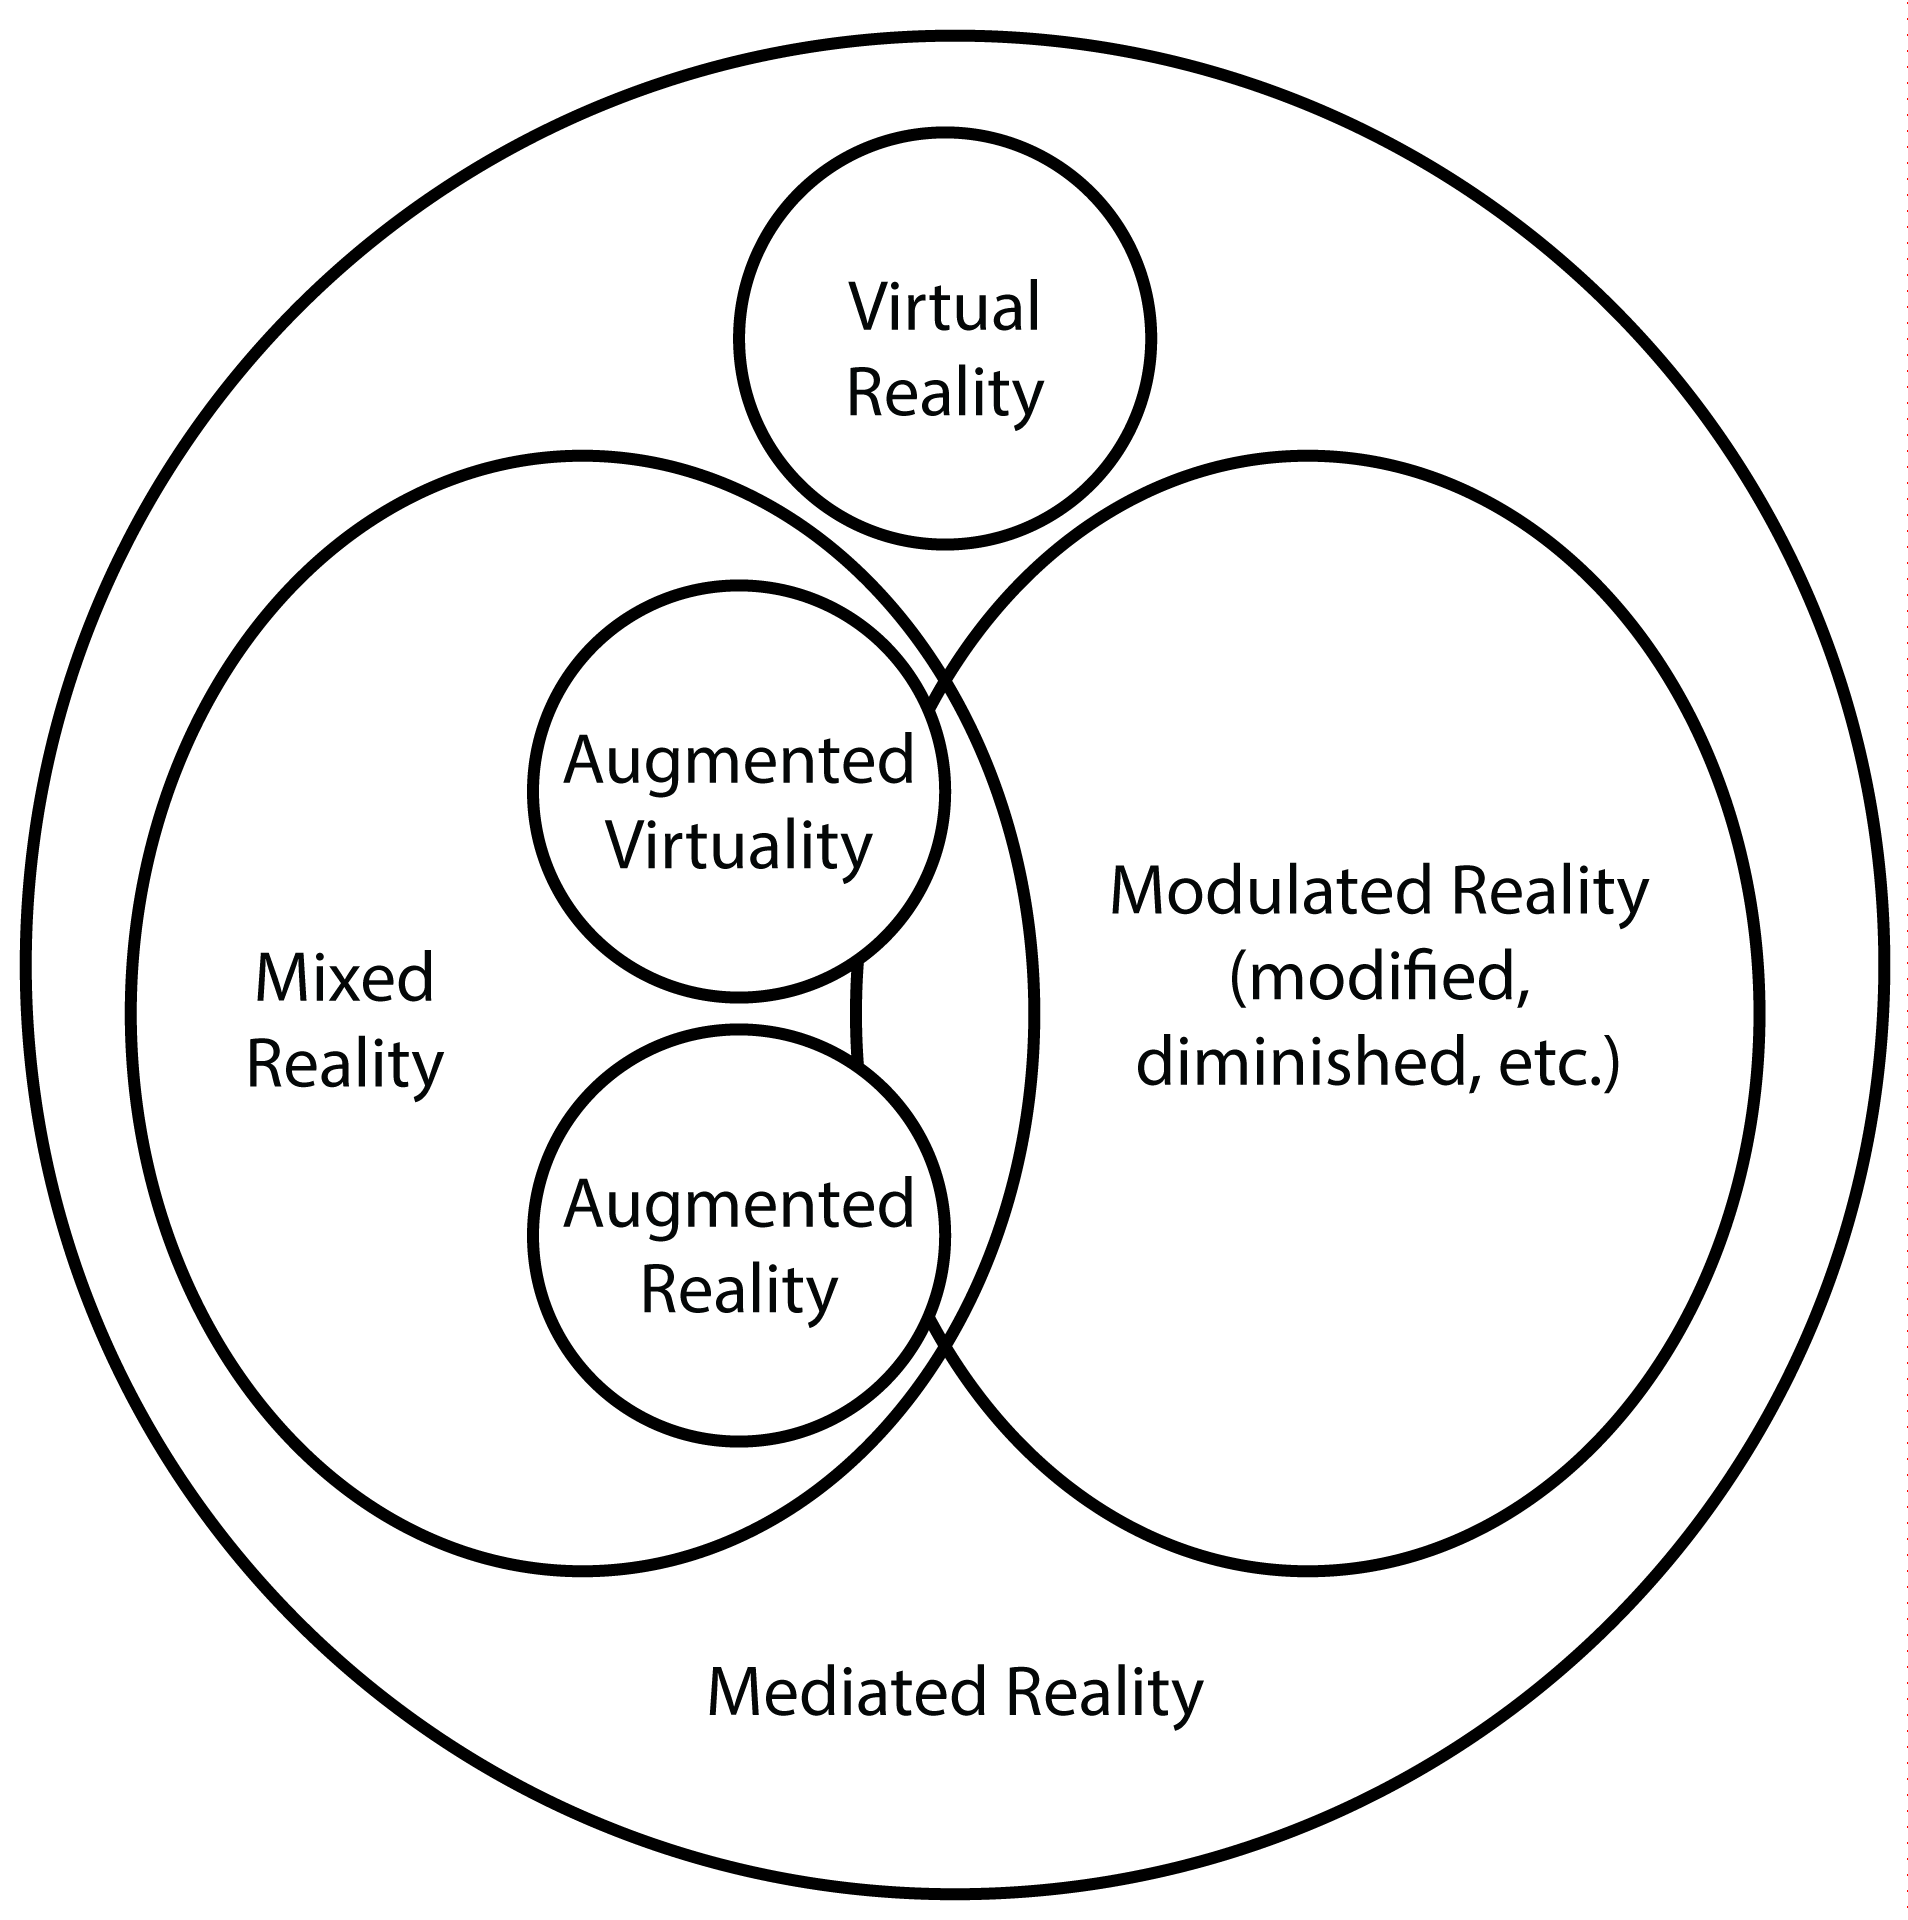
\includegraphics[width=0.95\linewidth]{Mann_venn_mod_1.png}
    \caption{Modified Mann venn diagram.}
    \label{Mann_venn_mod_1.png}
\end{minipage}
\end{figure}

Visualising the position of reality \& virtual reality using this same method requires more drastic alteration to the Venn diagram, but is diagnostic in further revealing the relationships between the terms introduced within Want's literature. The further modified Venn diagram (figure \ref{Mann_venn_mod_3.png}) shows;
\begin{itemize}
	\item mixed reality as the intersection of reality \& virtual reality;
	\item mediated reality can be comprised from purely real or purely virtual content;
	\item all virtual reality is necessarily mediated reality;
	\item modulated reality systems can comprise only mediated real, or of mixed reality;
	\item augmented reality \& augmented virtuality, can feature in modulated reality systems.
\end{itemize}

\begin{figure}[h]
\centering
  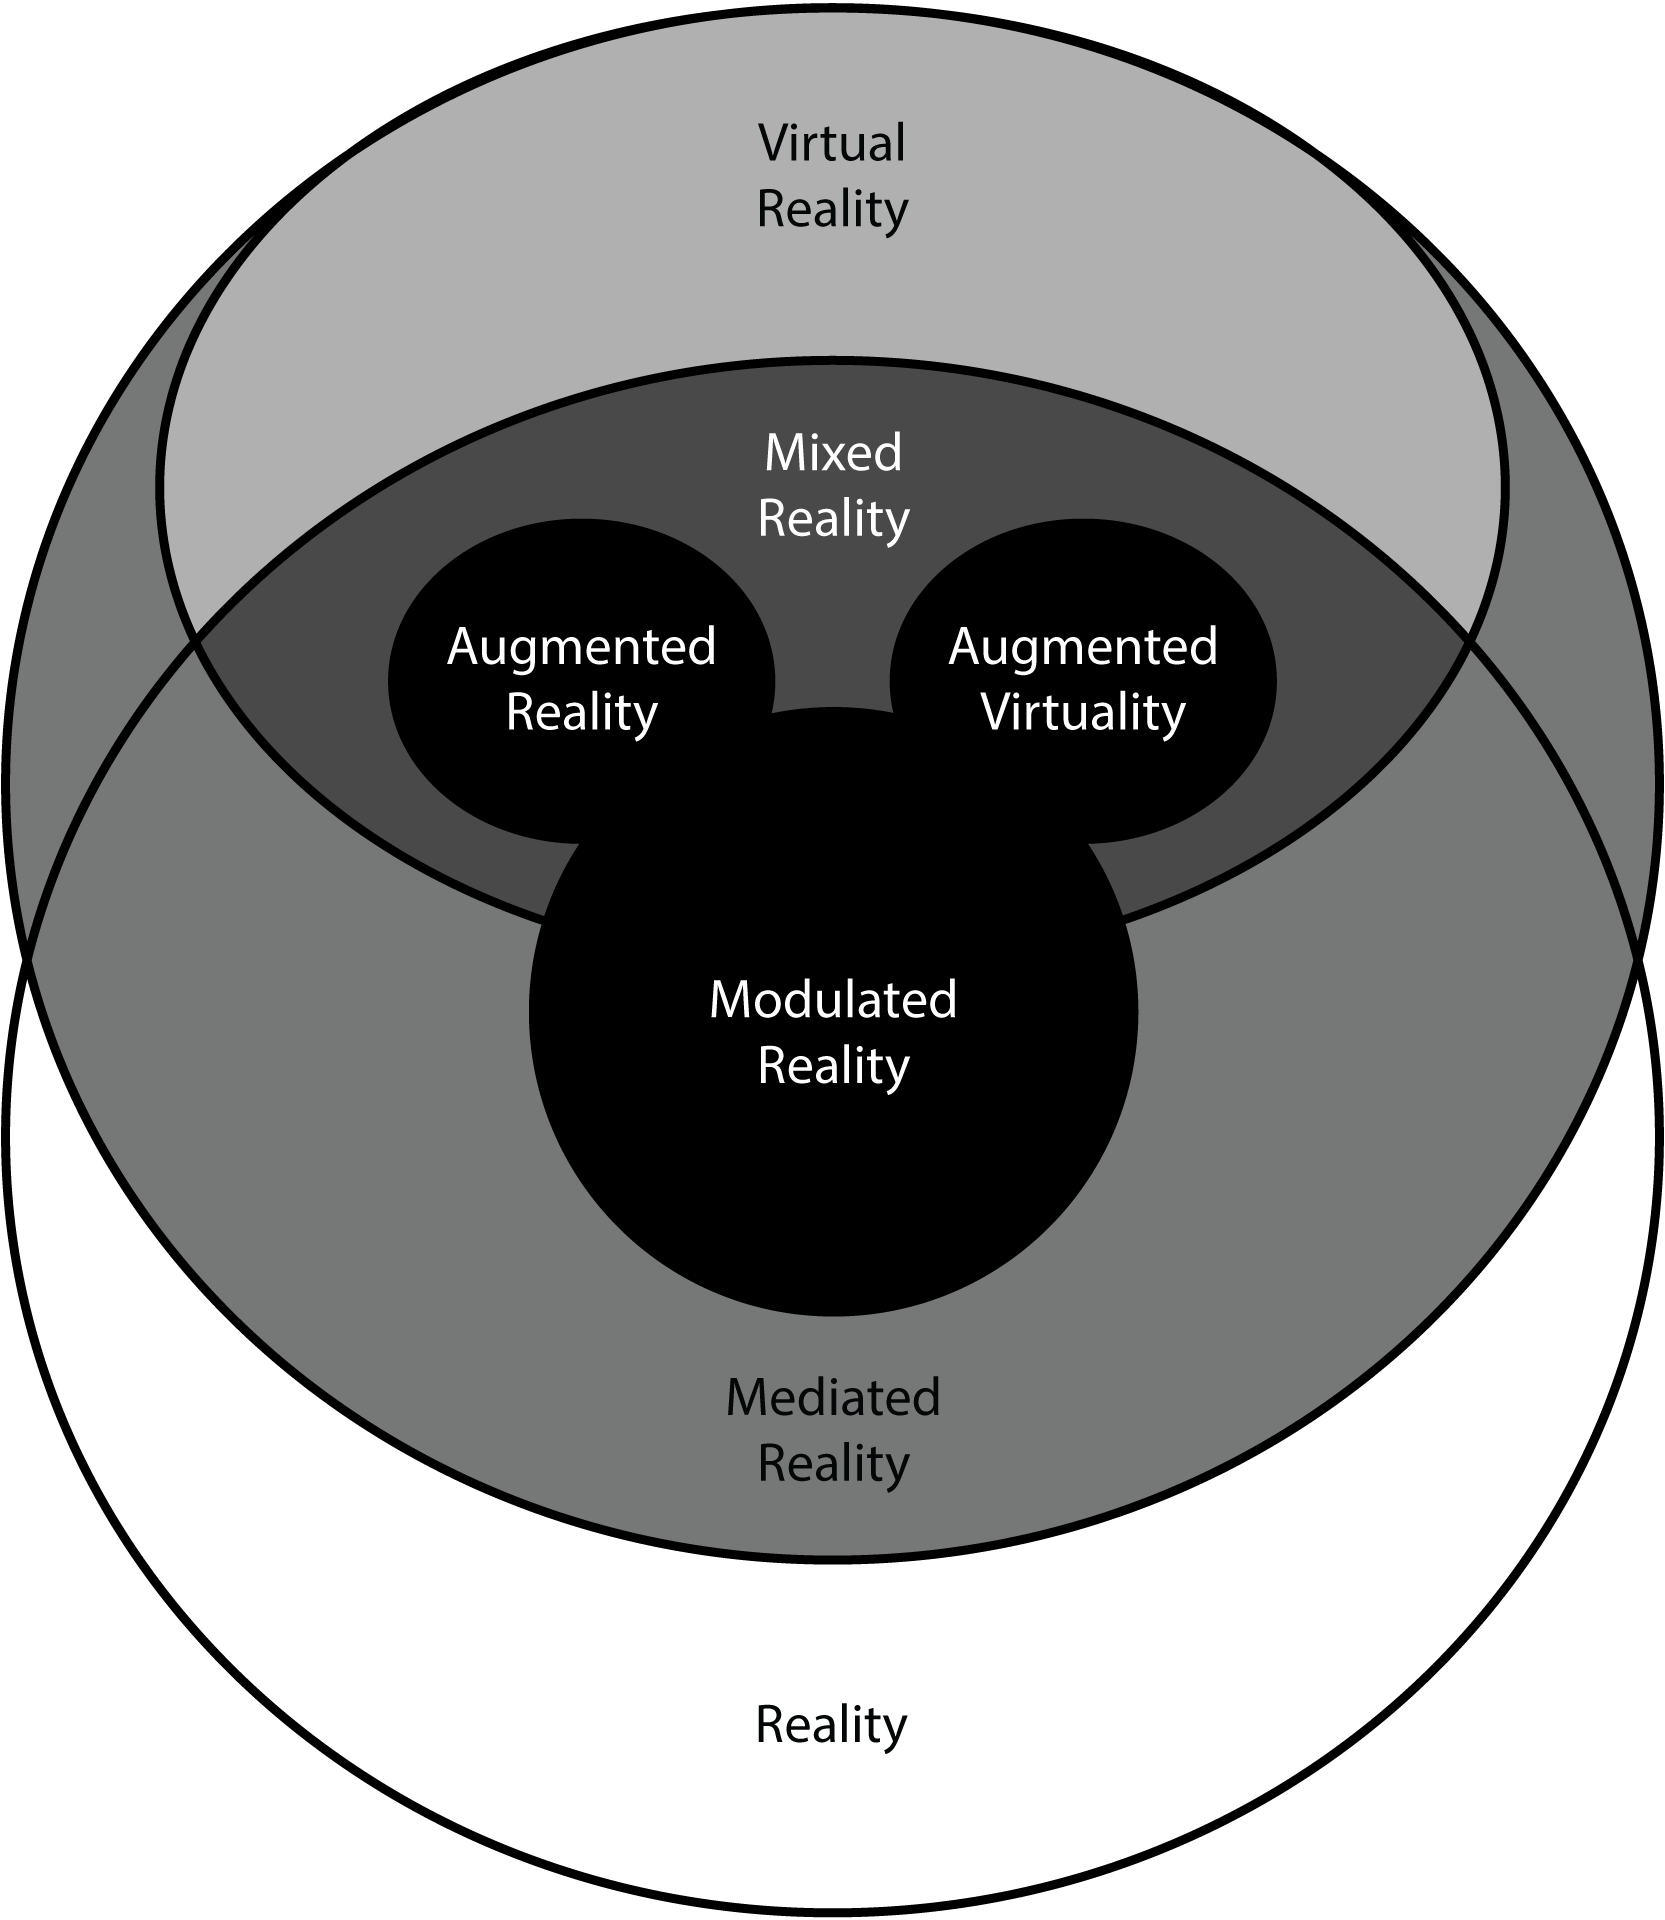
\includegraphics[width=0.5\linewidth]{Mann_venn_mod_3.png}
  \caption{Further modified Mann venn diagram.}
  \label{Mann_venn_mod_3.png}
\end{figure}

\textbf{Does this final Venn diagram not show that Modulated Reality can exist as Mixed Reality but which *isn't* either Augmented Reality or Augmented Virtuality though?}

%=========================================================================================================
%=========================================================================================================

\section{Adopted Definitions of Alternate Realities}

Following are the definitions \& identifying/classifying criteria for the different categories of alternate realities identified thus far in this chapter.

%This review has discovered differing (and in some cases conflicting) definitions for the different categories of alternate realities and for the criteria for differentiating between them. What follows in this section represents the definitions and differentiating criteria that this review has adopted after concluding them the most widely accepted and well reasoned.

%=========================================================================================================

\begin{center}
\begin{longtable}{| l | p{12cm} |}

\hline	
	
%=========================================================================================================
		
\textbf{Reality} & An environment that is entirely unmodelled, with the viewport containing no virtual objects and with no computer-based quantitative information associated with any of the (necessarily real) objects. \\
		
\hline
		
%=========================================================================================================
		
\textbf{Virtual Reality} & The polar opposite of \textit{reality}, an environment that consists solely of virtual objects, with computer-based quantitative information associated with all of them and between all of them, creating a completely synthetic world entirely discrete and separate from the real world; a new world that exists solely within the data structures of a computer. \textbf{***cite Milgram and Want***}

While traditional definitions of \textit{virtual reality} require the environment to be completely immersive, such that when involved with the environment the user is completely unaware of the real environment that surrounds them (eg by using Head Mounted Displays \& body tracking techniques to remove logical anchors to the real world~\cite{Druck2006}) the criteria adopted herein are less drastic, classifying the virtual environments presented by video games viewed via 2D monitors as rudimentary implementations of virtual reality; they are completely modelled environments that exist entirely separate to the real world. \\
		
\hline
		
%=========================================================================================================

\textbf{Mixed Reality} & The broad range of environments that arise from the merging of real and virtual environments to some extent such that the result is neither entirely real nor entirely virtual, where real and virtual objects co-exist. Both \textit{augmented reality} and \textit{augmented virtuality} are included under the broader classification of \textit{mixed reality}. \\

\hline
		
%=========================================================================================================

\textbf{Augmented Reality} & A mixed reality environment comprising a real environment has had virtual objects added to or overlain upon it. A common approach for achieving this addition/overlay is superimposing virtual objects over a direct or indirect view of the real environment using Head Mounted Displays \&/or cameras~\cite{Krevelen2010}. \textbf{***better citation here pls, there was that big AR survey paper***} \\

	%A commercial example of \textit{augmented reality} is the Layar browser for mobile phones, which overlays various forms of data onto the view captured by a phone's camera after determining its location and orientation using GPS, accelerometer and magnetometer readings~\cite{eishita:layar}

%~\cite{Milgram1999}

\hline

%=========================================================================================================

\textbf{Augmented Virtuality} & A virtual environment upon which sampled real objects are overlain, perhaps through the use of cameras~\cite{caballero:behand}. \\

%A simple commercial example of augmented virtuality is the EyeToy accessory and associated software for Sony's Playstation 2 games console (and later the Playstation Eye for the Playstation 3), a digital camera that captures images of players and their surroundings and integrates them into the gaming experience presented on the screen.

\hline

%=========================================================================================================

\textbf{Mediated Reality} & Write after reading Mann document again. \\

\hline

%=========================================================================================================

\textbf{Modulated Reality} & Write after reading Mann document again. \\

%=========================================================================================================

\hline

\end{longtable}
\end{center}

%=========================================================================================================
%=========================================================================================================

\section{Cross Reality}

Cross reality is the ubiquitous mixed reality situation that arises from the fusion of real-world sensor/actuator infrastructure with virtual environments, such that augmented reality and augmented virtuality manifest simultaneously and facilitate synchronous multi-directional exchange of media and control information between real and virtual environments. Sensors collect and tunnel dense real-world data into virtual environments where they are interpreted and displayed to dispersed users, whilst interaction of virtual participants simultaneously incarnates into the real world through a plenitude of diverse displays and actuators~\cite{Paradiso2009}.

The principle features that distinguish cross reality from the other alternate realities covered by this chapter are;
\begin{enumerate}
	\item a shift from single- to bi-directional information flow between real and virtual environments~\cite{kim:practical}
	\item that both environments are complete unto themselves (but are enriched by their ability to mutually reflect, influence and merge into one another).~\cite{lifton:merging}
\end{enumerate}

\textit{This thesis presents systems that focus on the second aspect above \& extends it by permitting both environments to be experienced at any time \& position.}

%=========================================================================================================

\subsection{The History of Cross Reality}

Cross reality was realised \& developed as a research area by the Responsive Environments Group at MIT's Media Lab, centred around the research of Joshua Lifton~\cite{Lifton2007a} in combining the Plug sensor/actuator platform~\cite{Lifton2007b} with a Second Life hosted virtual model of the physical Lab in the `Shadow Lab' project. These projects furthered initial work by the IBM Virtual Universe Community~\cite{Hughes2006, Hughes2006a,Hughes2006b}, whose progress toward a cross reality platform was confirmed via personal correspondence;

\begin{quote}
\textit{``The control mechanisms worked two ways generally. There was a physical lab that had devices that were controlled by a pub/sub mechanism based on the light weight protocol MQTT. Those devices subscribed to various messages. So initially web pages controlled them \ldots\ Equally the objects generated messages when they were physically switched on and off. As SL had an RPC interface it was possible \ldots\ to subscribe to the same messages and send requests into SL to change states of object \ldots\ So there were lights, blinds, proximity detectors and even the tilt sensors on the laptops that were instrumented with these messages.''}
\end{quote}

\begin{figure}[h]
\centering
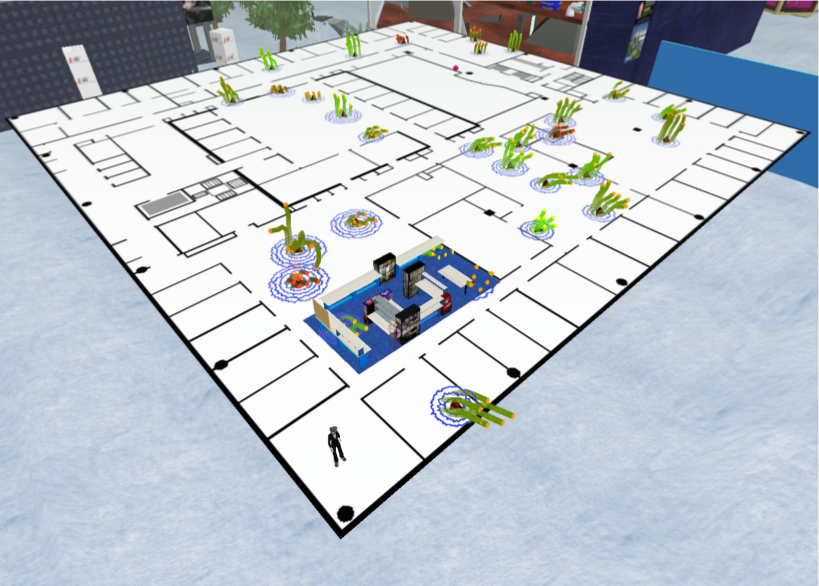
\includegraphics[width=\textwidth]{lifton_shadow_lab.png}
\caption{Side view of the Shadow Lab platform, showing a reconstruction of part of the Media Lab, virtual `data ponds' where Plug sensor/actuator devices were place \& a human-sized avatar.}
\label{lifton_shadow_lab.png}
\end{figure}

The Shadow Lab did not allow for tandem visual engagement with both constituent environments of the cross reality platform.

The Ubiquitous Sensor Portal project that followed the Dual Reality Lab partially addressed this, by situating 45 I/O rich `portals', shown in figure \ref{ubiquitous_sensor_portal.jpg}, throughout the Media Lab, each with a corresponding extension in Second Life. However in stark contrast to the Dual Reality Lab, the virtual portals were not situated in a simulation of the real Media Lab in situations corresponding to their physical location, but instead used a more abstract virtual representation with a geometric layout; this design, shown in figure \ref{ubiquitous_sensor_portal_virtual.png}, reflected intellectual affiliation as opposed to real-world locationHowever in stark contrast to the Dual Reality Lab, the virtual portals were not situated in a simulation of the real Media Lab in situations corresponding to their physical location, but instead used a more abstract virtual representation with a geometric layout; this design, shown in figure \ref{ubiquitous_sensor_portal_virtual.png}, reflected intellectual affiliation as opposed to real-world location

\begin{figure}[h]
\centering
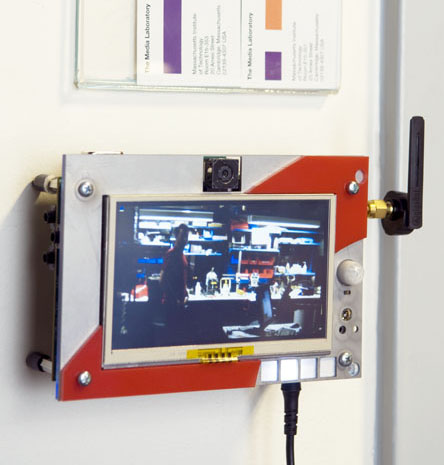
\includegraphics[width=0.6\textwidth]{ubiquitous_sensor_portal.jpg}
\caption{A Ubiquitous Sensor Portal.}
\label{ubiquitous_sensor_portal.jpg}
\end{figure}

%=========================================================================================================

\subsection{The Vacancy Problem}

Lifton identifies the `vacancy problem';
\begin{quote}
\textit{``the noticeable and profound absence of a person from one world, either real or virtual, while they are participating in the other. Simply put, the vacancy problem arises because people do not currently have the means to be in more than one place (reality) at a time.''}
\end{quote}
as a fundamental characteristic of the current generation of virtual worlds and proposes dual reality, more closely linking the real world with the virtual world, as an approach to mitigate the problem.

%=========================================================================================================

\subsection{Lifton's Virtual Worlds Taxonomy}

As the prominent figure in the development of the cross reality paradigm it is worth comparing Joshua Lifton's definitions for different categories of alternate realities and the relationships between them~\cite{Lifton2007a} in the current context.

Lifton's definitions, or more accurately his relationships between, the terms \textit{reality}, \textit{augmented reality}, \textit{mixed reality} and \textit{virtual reality} do not perfectly match the consensus that this review has observed. Lifton defines the terms individually in agreement with the consensus, however doesn't proffer the conclusion that mixed reality is a broad term that includes augmented reality. He also doesn't mention augmented virtuality, even though his cross reality projects could be construed as implementing it. Finally his diagram that alludes to Milgram's continua and is included as figure \ref{original_lifton_axis.png}, situates mixed reality at an incorrect position, implying that Lifton's definition of mixed reality is of a discrete state to that of augmented reality, even though his textual definition of mixed reality hints that it logically encompasses augmented reality. This review presents a modified version of Lifton's diagram to illustrate these differences as figure \ref{modified_lifton_axis.png}.

Lifton does however explain that while such a taxonomy can be successfully applied to most alternate reality efforts, it does not well address the concept of cross reality where there are two complete realities, one real and one virtual. \textbf{***is there a direct citation for this?***}

\begin{figure}[h]
	\centering
	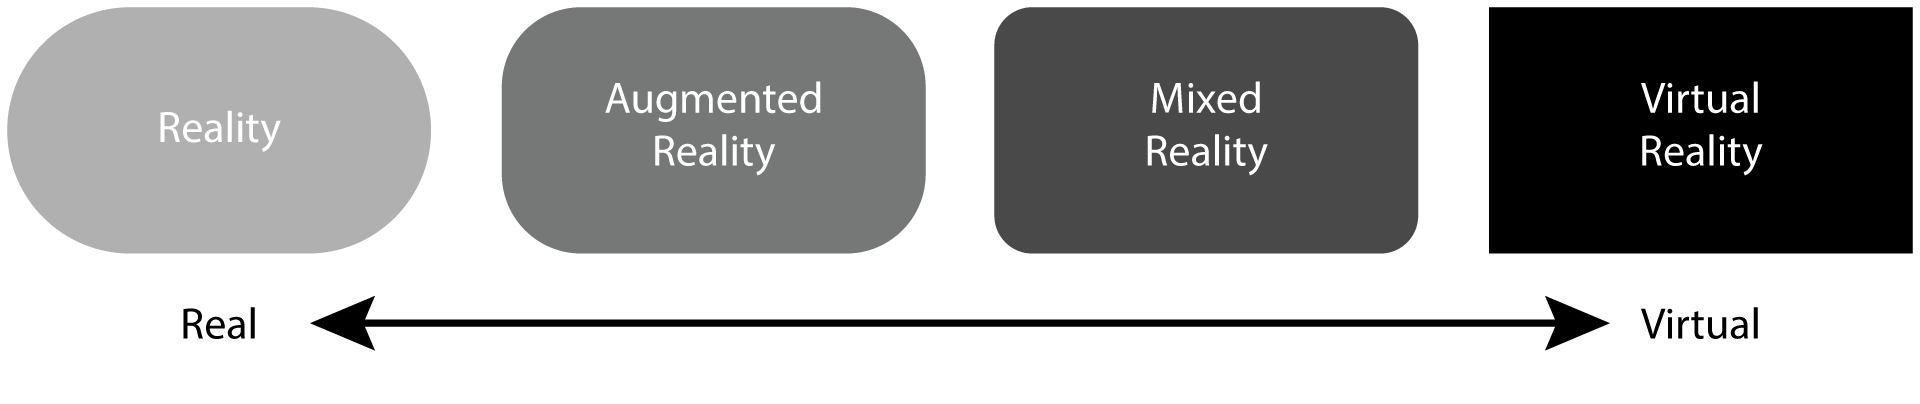
\includegraphics[width=.8\textwidth]{Lifton_continuum_original.png}
	\caption{The \textit{``virtual worlds taxonomy as viewed on the real-virtual axis''} presented by Lifton.}
	\label{original_lifton_axis.png}
\end{figure}

\begin{figure}[h]
	\centering
	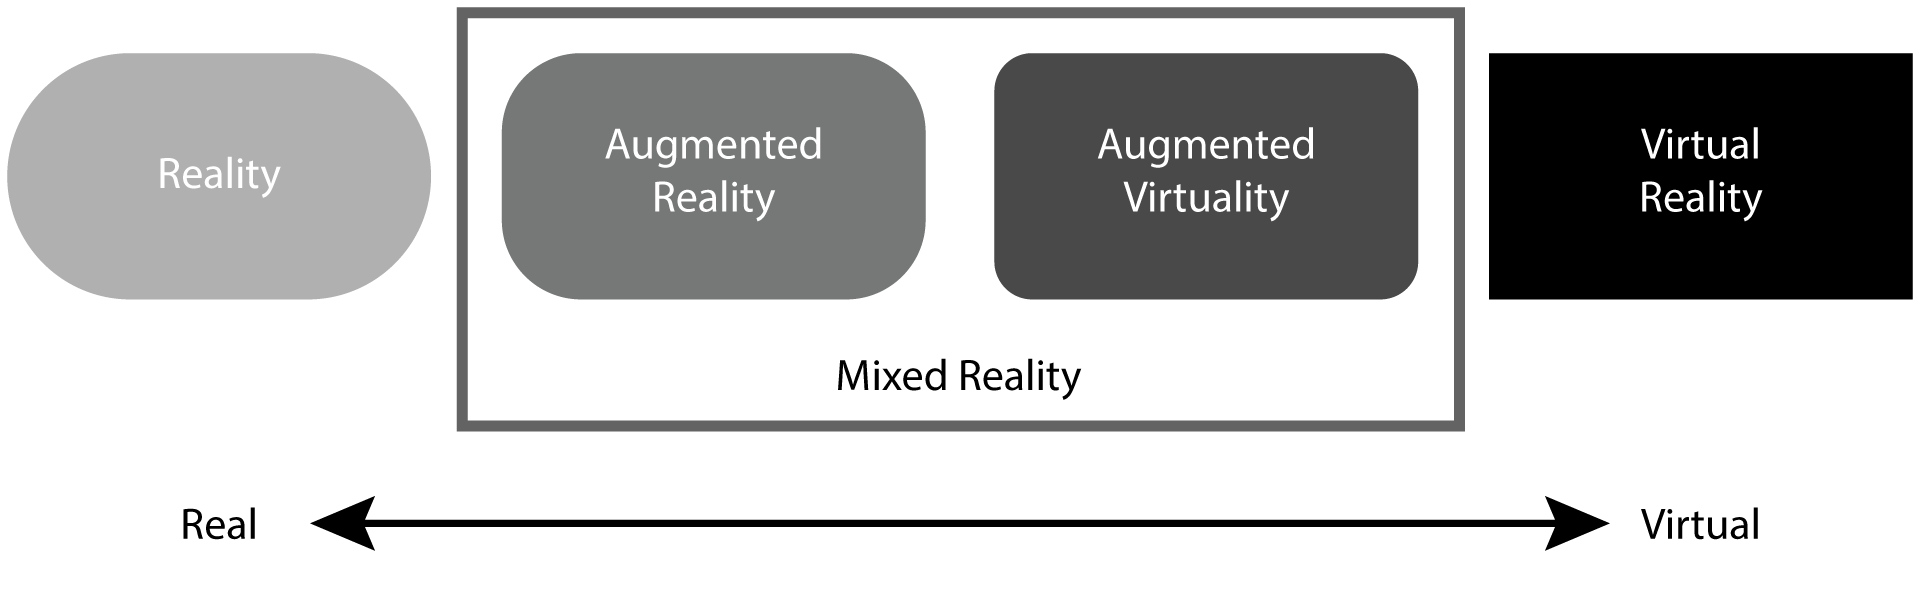
\includegraphics[width=.8\textwidth]{Lifton_continuum_modified.png}
	\caption{Lifton's taxonomy as modified by this review.}
	\label{modified_lifton_axis.png}
\end{figure}

%=========================================================================================================

\clearpage

\subsection{Cross Reality \& Milgram \& Kishino's Reality-Virtuality Continuum}

The position of XR in relation to other alternate realities studied by Computer Science can be visualised using Milgram \& Kishino's \textit{virtuality continuum} that stretches from an entirely real environment at one extreme to an ontologically parallel but entirely virtual environment~\cite{Qvortrup2002} at the other. The explanation herein distinguishes between environments themselves (depicted in figures \ref{virtuality-continuum-augmented-reality} to \ref{virtuality-continuum-cross-reality-3} by solid ellipses) \& where the stimuli that the user is perceiving originate from (depicted by dashed ellipses).

%Ontology - The core meaning within computer science is a model for describing the world that consists of a set of types, properties, and relationship types. There is also generally an expectation that the features of the model in an ontology should closely resemble the real world (related to the object).

Of particular importance is to appreciate the distinction between a XR system \& an \textit{augmented reality} (AR) system, as both concepts involve user engagement with both real \& virtual content. Whilst an AR system features a single environment, comprised of the user's RW overlain by some virtual content, with the user perceiving stimuli from this single augmented environment (figure \ref{virtuality-continuum-augmented-reality}), a XR system instead features two discrete environments, one real \& the other virtual, each complete unto itself (figure \ref{virtuality-continuum-cross-reality-1}).

Whilst AR falls within the realms of Mixed Reality (MR), a XR system can be considered as occupying the two extremes of the continuum outwith the MR region. However, XR systems that allow simultaneous interaction with both of their constituent environments blur this definition; using a XR platform such as that discussed in this document, a user can transition between perceiving stimuli from each of these environments (figures \ref{virtuality-continuum-cross-reality-2} \& \ref{virtuality-continuum-cross-reality-3}) in a manner that allows them to engage with each environment without becoming wholly vacant from the other.

\begin{figure}[h]
	\begin{center}
		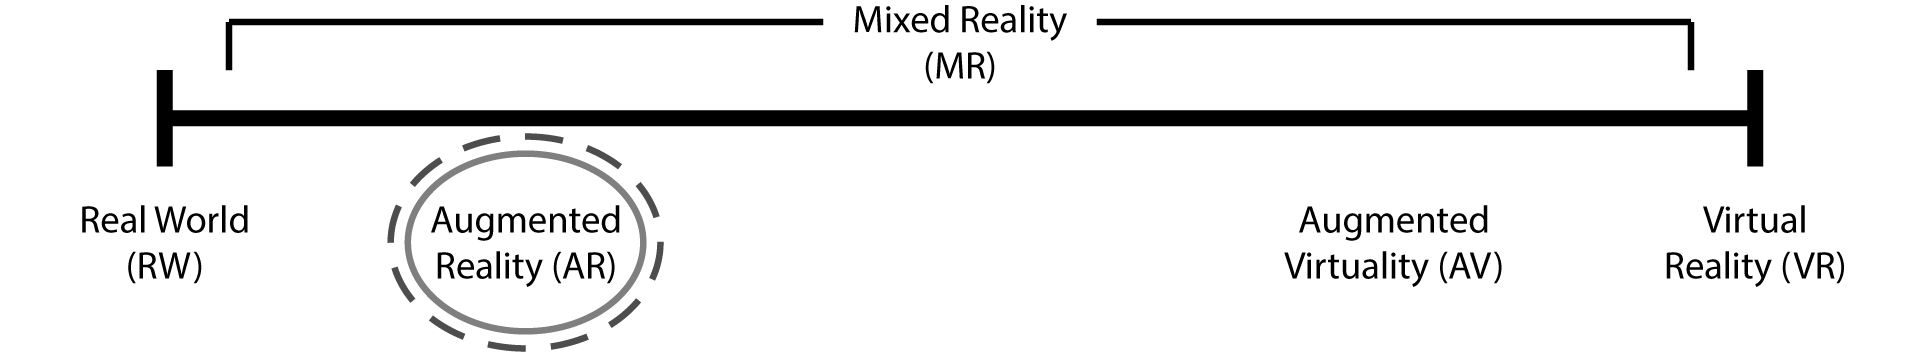
\includegraphics[width=\textwidth]{virtuality-continuum-augmented-reality.png}
		\caption{AR visualised using the virtuality continuum.}
		\label{virtuality-continuum-augmented-reality}
	\end{center}
\end{figure}

\begin{figure}[h]
	\begin{center}
		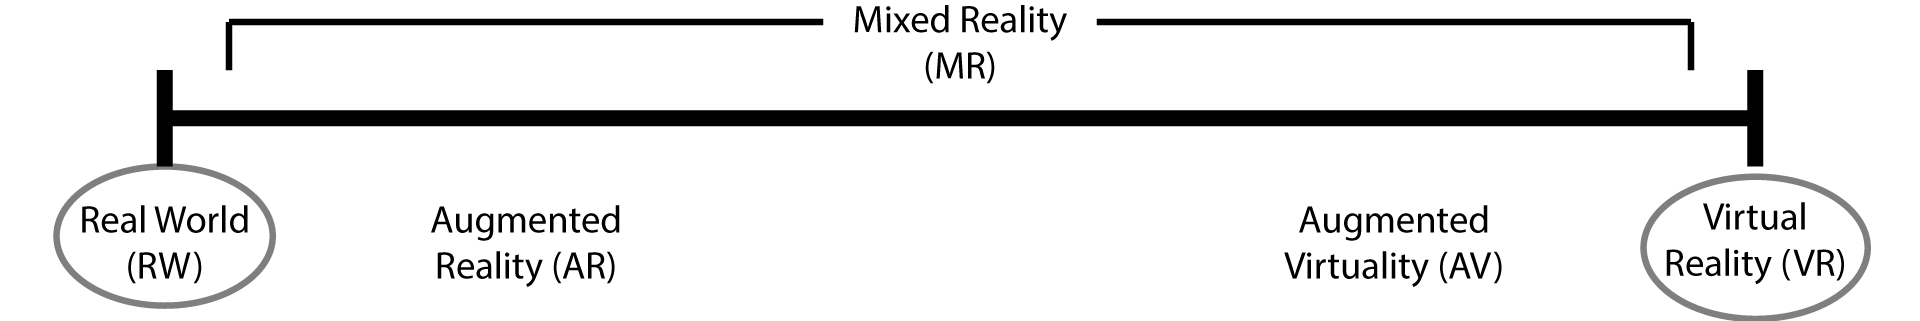
\includegraphics[width=\textwidth]{virtuality-continuum-cross-reality-1.png}
		\caption{The two environments that comprise a XR system.}
		\label{virtuality-continuum-cross-reality-1}
	\end{center}
\end{figure}

\textbf{Is it worth pointing out on the diagram that a true XR system would have a constant bi-directional stream of data between the two environments? And that without this, we have something like parallel reality?}

\begin{figure}[h]
	\begin{center}
		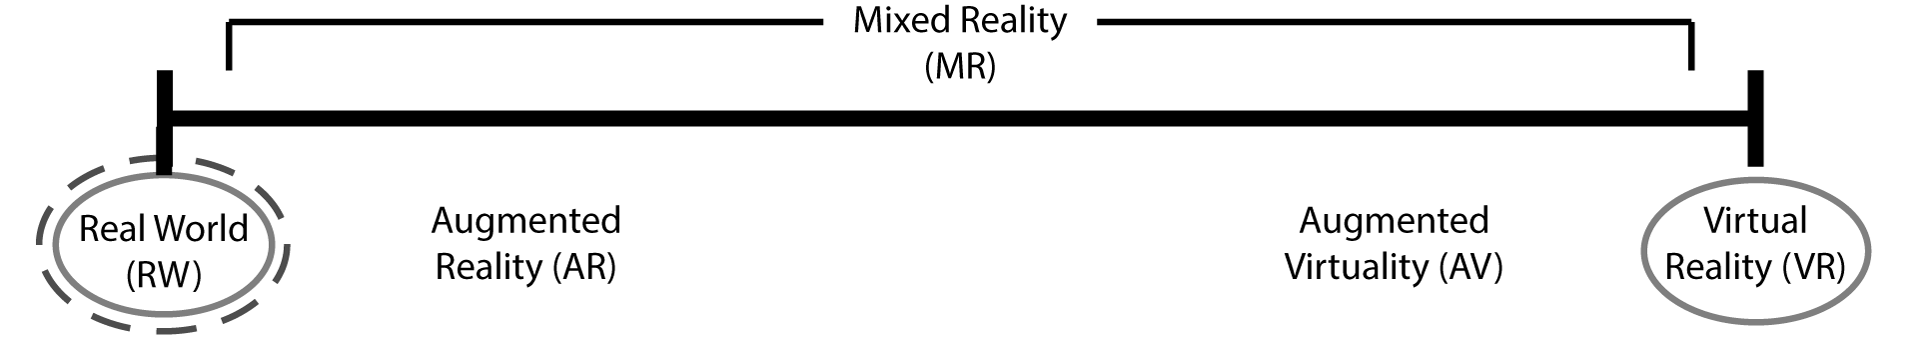
\includegraphics[width=\textwidth]{virtuality-continuum-cross-reality-2.png}
		\caption{A XR system with the user attending to RW stimuli.}
		\label{virtuality-continuum-cross-reality-2}
	\end{center}
\end{figure}

\begin{figure}[h]
	\begin{center}
		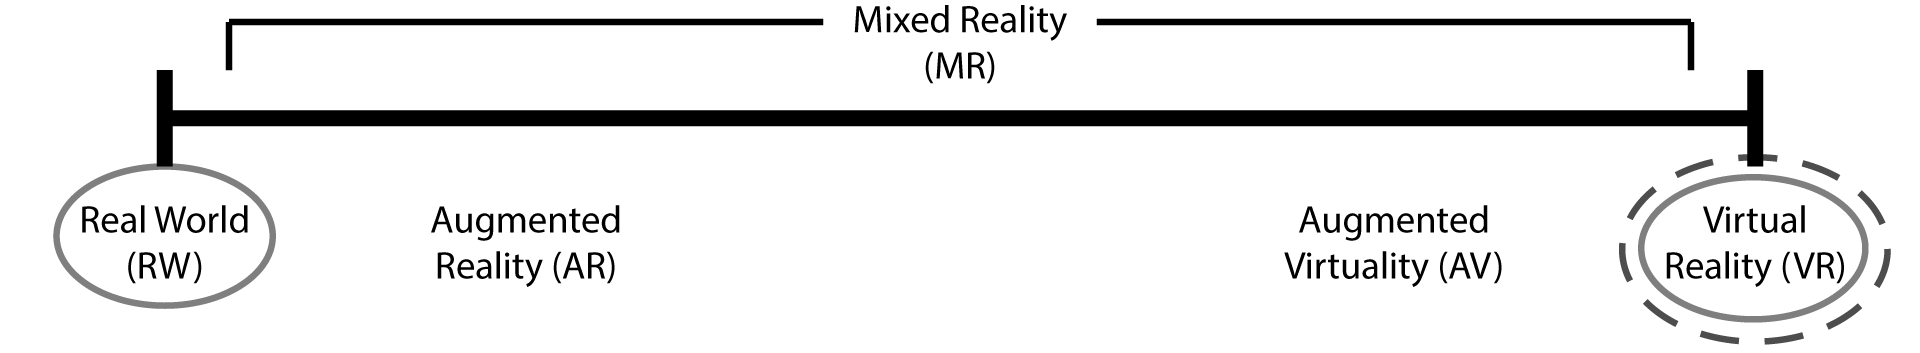
\includegraphics[width=\textwidth]{virtuality-continuum-cross-reality-3.png}
		\caption{A XR system with the user attending to VR stimuli.}
		\label{virtuality-continuum-cross-reality-3}
	\end{center}
\end{figure}

\begin{figure}[h]
	\begin{center}
		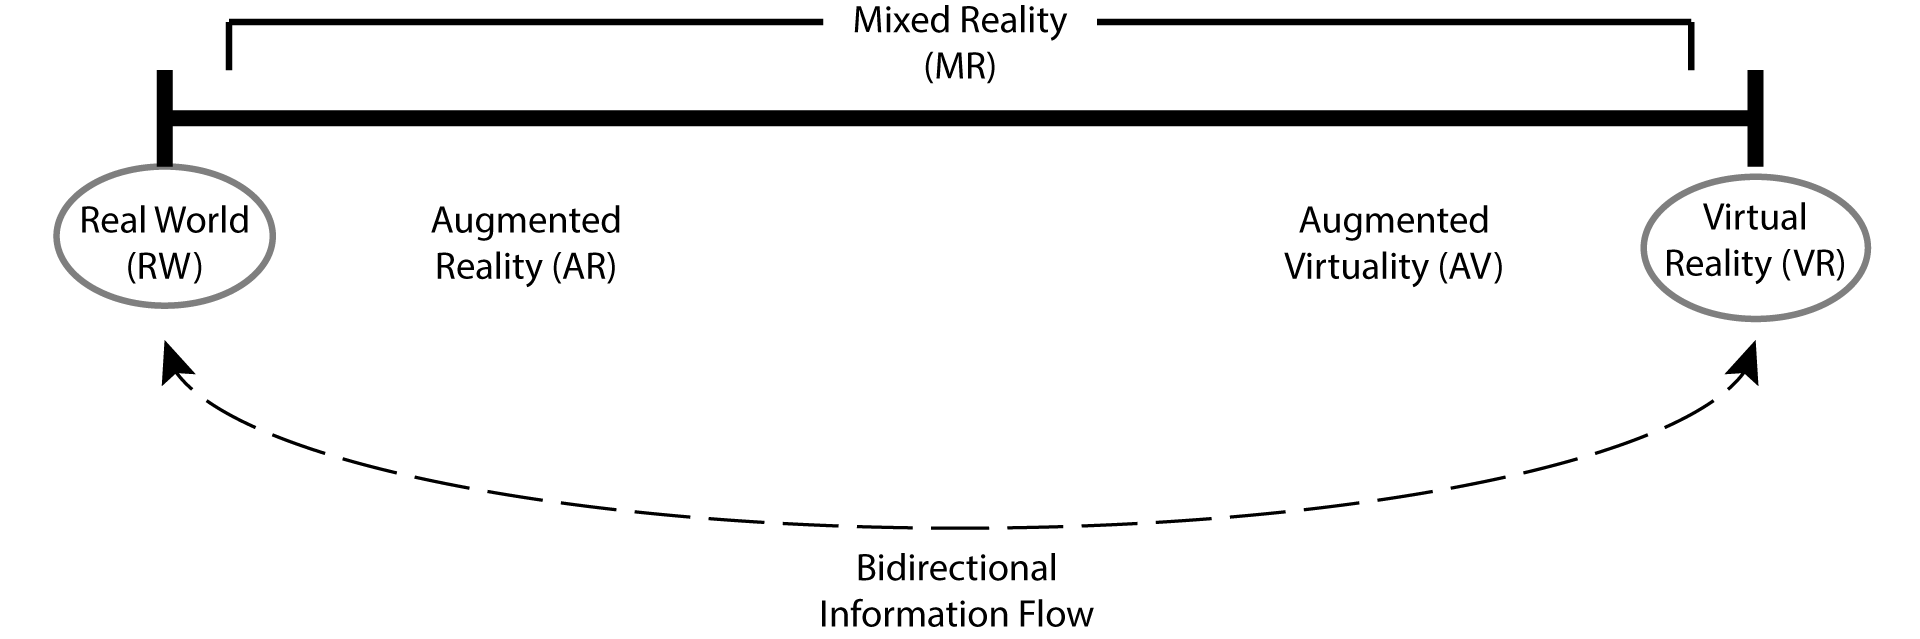
\includegraphics[width=\textwidth]{virtuality-continuum-cross-reality-information-flows-dashed.png}
		\caption{The two environments that comprise a XR system, plus the bidirectional information flow between them.}
	\end{center}
\end{figure}

%=========================================================================================================

\subsection{PolySocial Reality in Cross Reality Systems}

%=========================================================================================================
%=========================================================================================================

\section{On Presence}

\subsection{Combined Milgram \& Kishino continuum/Waterworth \& Waterworth three dimensions of virtual experience model}

\newcommand{\presencefootnote}{\footnote{\textbf{Presence} in this context is defined as a state of heightened perceptual processing of environmental stimuli (\textit{``a psychological focus on direct perceptual processing''}~\cite{Waterworth2001}) accompanied by lessened conceptual reasoning, whether these environmental stimuli originate from a real environment, a virtual environment, a mixed reality environment, or even from multiple discrete environments.}}

\newcommand{\absencefootnote}{\footnote{\textbf{Absence} is defined as \textit{``a psychological focus on \ldots conceptual processing''}~\cite{Waterworth2001}.}}

The virtuality continuum is here considered to be analogous to the \textit{locus of attention} axis of Waterworth \& Waterworth's \textit{three dimensions of virtual experience} model~\cite{Waterworth2001}; the combination of these models is shown by figure \ref{focus-locus-sensus-with-virtuality-continuum}. In this model, locus of attention represents the environment where the stimuli that the user is perceiving originate from; focus of attention represents the balance between conceptual/abstract reasoning \& perceptual/concrete processing, where complex conceptual reasoning results in little attention being paid to processing environmental percepts (whether originating from real or virtual stimuli) thus reducing presence\presencefootnote{} in that environment toward its antithesis $-$ absence\absencefootnote{}; and sensus of attention represents the level of conscious arousal (or `wakefulness'~\cite{Laureys2009}) of the user, whether directed toward percepts originating from real stimuli, virtual stimuli, a mix, or not directed toward any percepts in the case of completely `absent' conceptual reasoning.

\begin{figure}[h]
	\begin{center}
		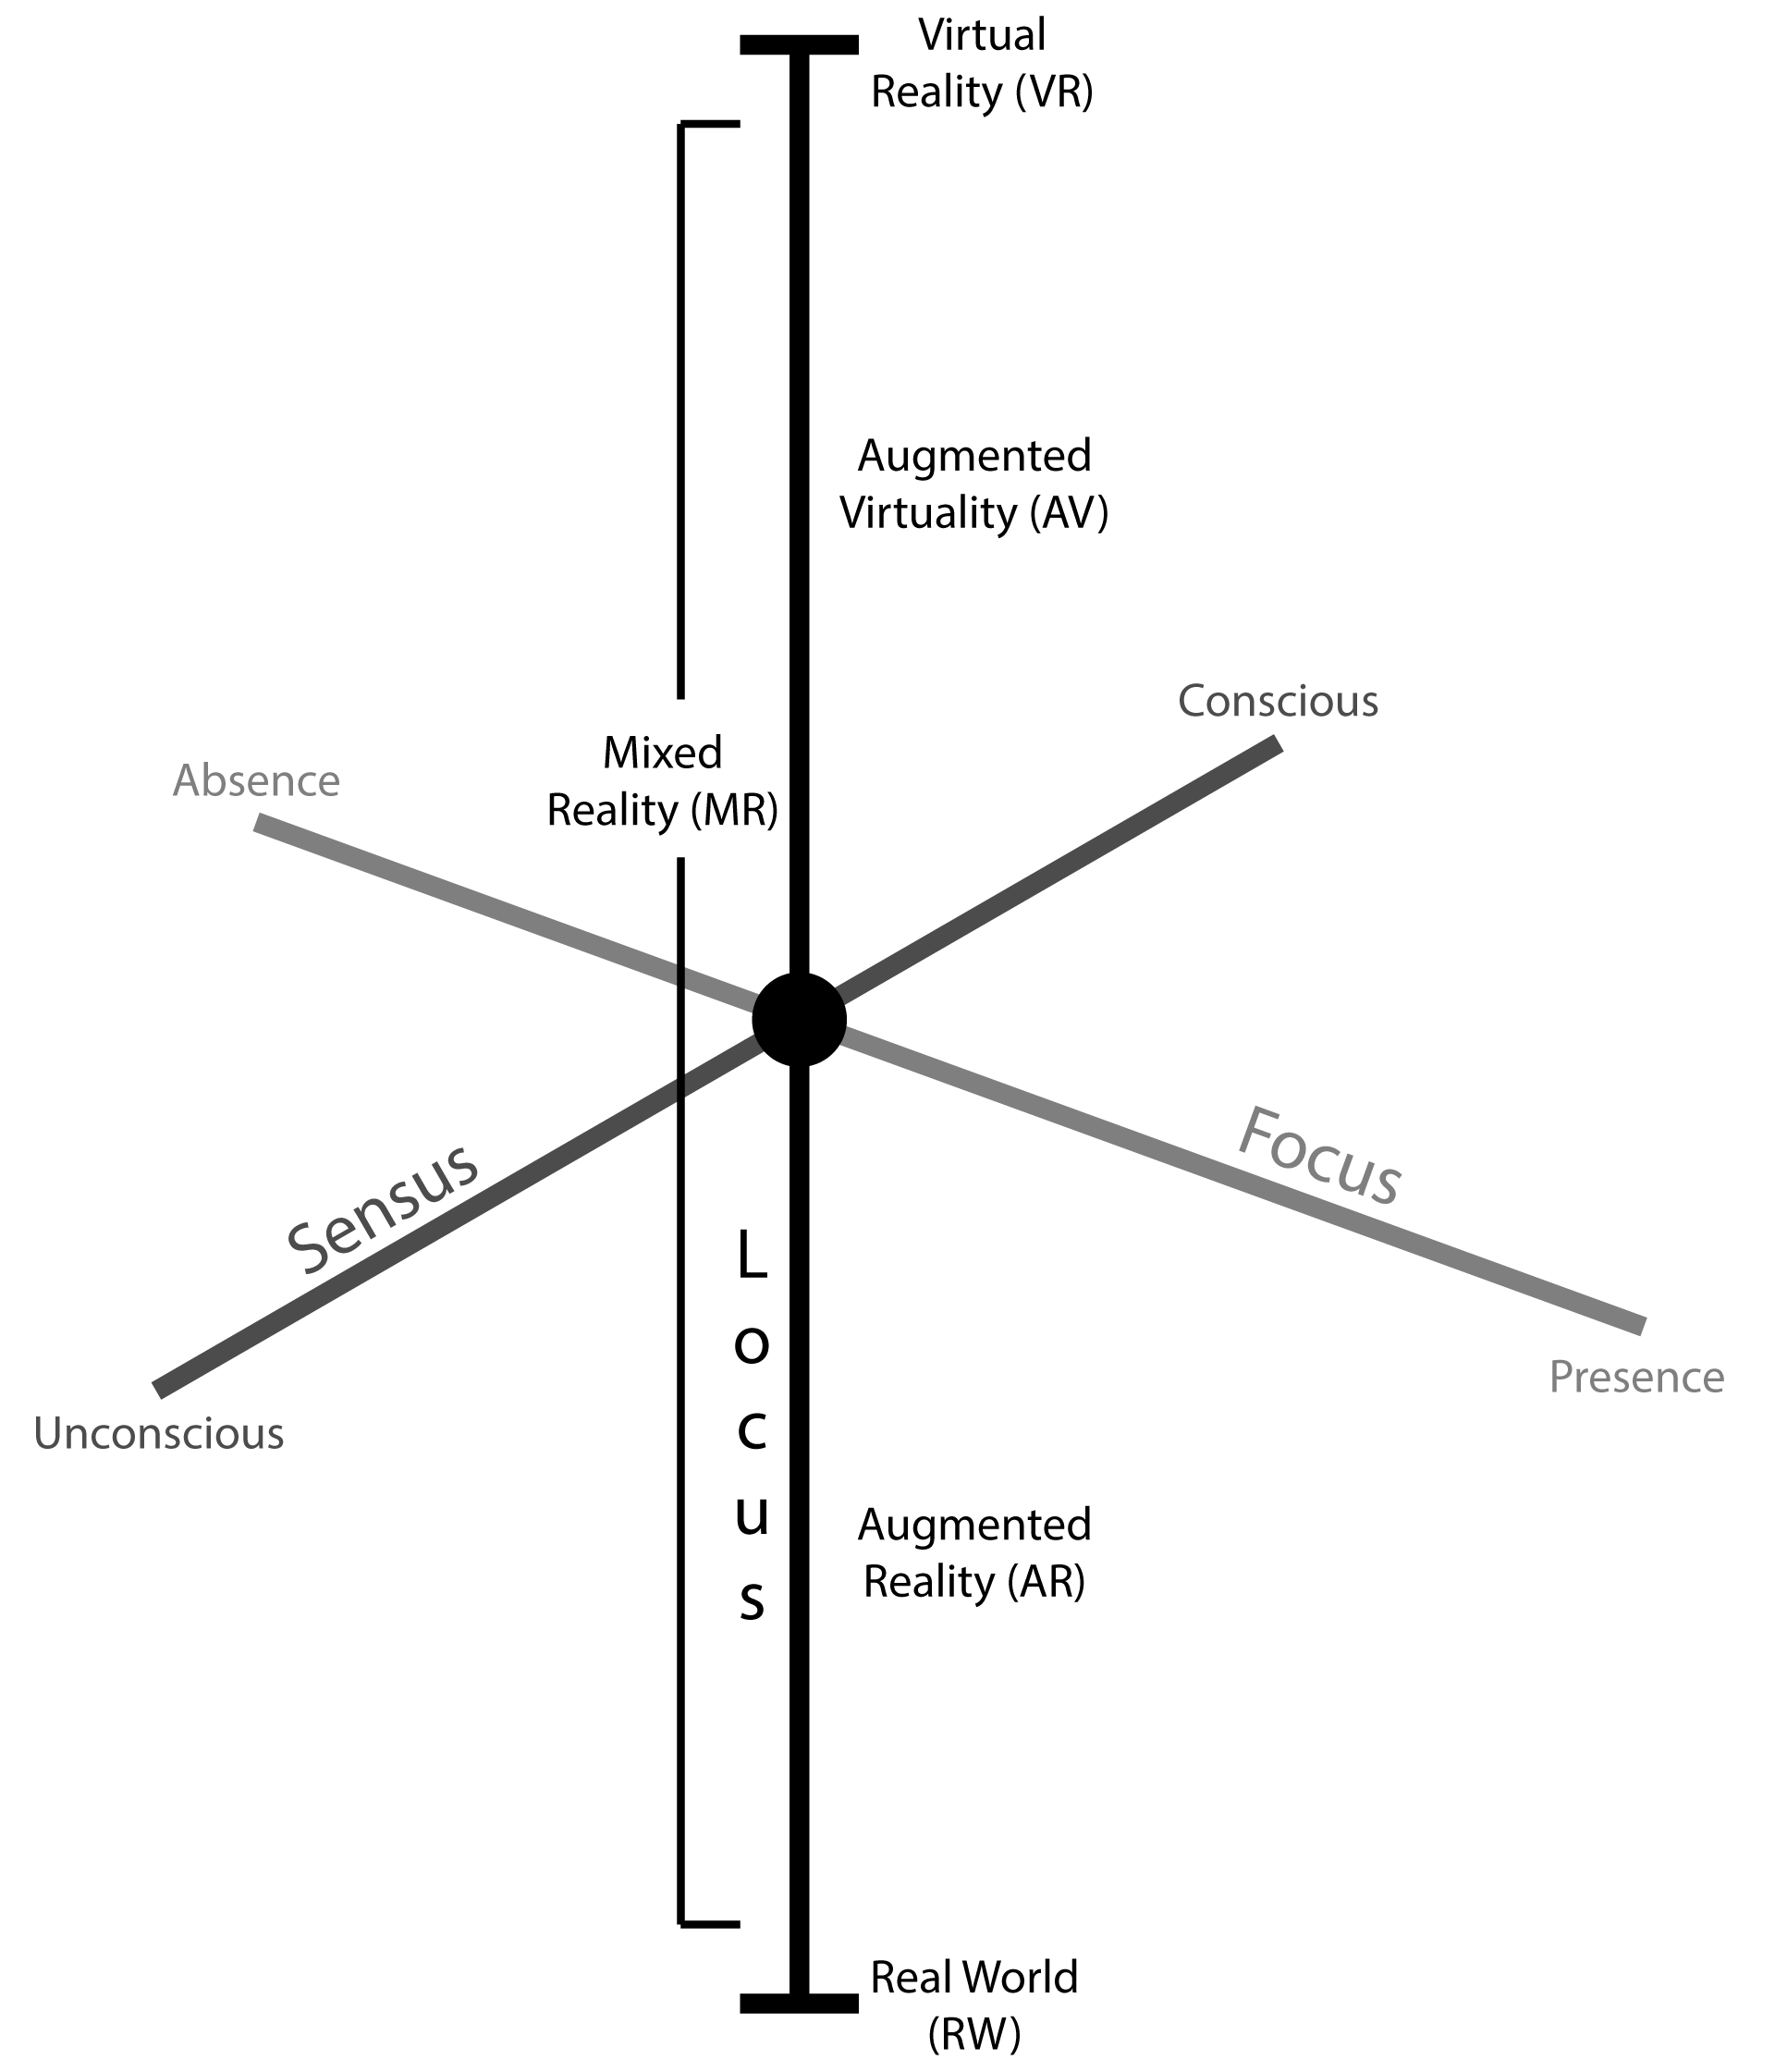
\includegraphics[width=0.7\textwidth]{focus-locus-sensus-with-virtuality-continuum.png}
		\caption{The combined virtuality continuum/three dimensions of virtual experience model.}
		\label{focus-locus-sensus-with-virtuality-continuum}
	\end{center}	
\end{figure}

%The Sensus Dimension - the importance of being awake in class
%"Even as we sleep dreamlessly..." (example of being 'unconscious' in this regard)

%fourth axis is alterity, between hermeneutics \& embodiment

%=========================================================================================================
%=========================================================================================================

\section{Parallel Reality visualised using the combined model}

\newcommand{\breakinpresencefootnote}{\footnote{The definition of \textbf{break in presence} adopted herein is the second from Waterworth \& Waterworth~\cite{Waterworth2001} (p205): a movement along the focus axis away from presence in the real or a virtual environment \& toward absence. This differs to Slater \& Steed's original definition in~\cite{Slater2000} as they considered presence only in terms of attending to stimuli from a virtual environment, with a break in presence as a Gestalt switch to instead attending to stimuli from the real environment. Waterworth \& Waterworth's model considers presence in terms of attending to stimuli from either the real \textit{or a virtual} environment, with a break in presence representing absence in the sense of heightened conceptual load \& the resultant reduced perceptual processing of environmental stimuli originating from \textit{either} the real or a virtual environment. This definition better fits the situation invoked by the Mirrorshades platform, which is concerned with intentionally \& willingly switching engagement between stimuli from both real \& virtual environments, rather than engaging with stimuli from only a virtual environment in a scenario where stimuli from the real environment are considered a `distraction'.}}

The novel aspect of the Mirrorshades platform is the ability it imparts upon its user to switch their locus of attention between equivalent vantage points in RW \& VR environments whilst walking around. This is achieved by the user performing transitions between RW visual stimuli \& VR visual stimuli, both presented via their HMD. This extends existing XR research by allowing the user to engage with the visual stimuli of the VR component of a XR system from any position \& at any time.

In order to achieve the highest quality of experience with this style of interaction with XR systems, it is vital to determine how best to implement these transitions; that is, to mitigate the increased cognitive load (manifesting as increased conceptual reasoning \& reduced perceptual processing, see section \ref{waterworth}) required to comprehend these transitions, as this increased cognitive load will detract from engagement with the environments \& reduce the user's willingness to perform these transitions.

Whilst some researchers support the notion that in systems where more than one environment competes for the user's locus of attention there is an `all or nothing' Gestalt switch between awareness of one environment \& the other~\cite{Slater2002}, which would result in a substantial increase in cognitive load upon each transition, Mirrorshades has been developed in support of the contrary opinion; that switching locus of attention from the stimuli of one environment to those of another does not completely overrule the user's awareness of the former, that both environments can be perceived at the same time (albeit one to a lesser extent)~\cite{Ijsselsteijn2001} \& that when engaging with VR content a user's focus can even be said to typically be \textit{shared} between VR \& RW~\cite{Waterworth2001}.

This latter position is particularly apt for situations wherein the RW \& VR environments share the same fundamental layout \& dimensions, as those in a XR system often do, as the inherent familiarity between the two environments reduces the cognitive load associated with transitioning between them. Furthermore, the notion of experience of presence as changing continually from moment-to-moment~\cite{Heeter2003, Ijsselsteijn1998} lends confidence to the successful mitigation of the cognitive load associated with these transitions to manageable levels. One might even liken this `switching' between RW \& VR to the `cycling through' behaviour observed in users of virtual communities, which stemmed from the `window' concept of modern computer operating systems~\cite{Turkle2004}.

However, no matter how smooth the transition the process is expected to always result in some heightened cognitive load, a temporary \textit{break in presence}\breakinpresencefootnote{} (BIP), as the user comes to terms with the new environment presented to them \& comprehends its relation to the other environment that they were just perceiving.

%\section{Transitions}
Transitions can be performed in multiple different manners \& it is hypothesized that users will prefer different styles of transition in different situations, surroundings \& scenarios (where `preference' toward a particular style of transition is expected to correlate strongly with a less severe BIP being experienced upon its execution).

To this end, several different transition methods have been developed \& this investigation will endeavour to identify \& quantify preferences toward them, to infer which approaches to transitioning between RW \& VR visual stimuli are more or less appropriate for the different situations that arise where a platform like Mirrorshades may be deployed. In particular, it is hypothesized that there will be a strong correlation between participant movement (or lack thereof) \& choice of particular transition style.

\subsection{Transitions using the Combined Model}
Visualised using the combined model (see section \ref{waterworth}) as figure \ref{focus-locus-sensus-with-virtuality-continuum-with-transition}, these transitions are an oscillation along the locus axis, between a RW environment at one position \& a VR environment at the other.

Heightened cognitive load required to comprehend a transition is a temporary movement upon the focus axis from presence toward absence (a BIP). With the ability of a wide FOV, stereoscopic 3D, head-tracked HMD to produce immersive VR visual stimuli that require fairly limited cognitive processing \& our inherent ability to engage with our RW surroundings without significant cognitive load, focus is expected to be high (toward the presence extremum) when attending to stimuli from either RW or VR.

Sensus is expected to be largely task dependent, however when performing a task that involves actively engaging with the visual stimuli from either/both of RW or VR it is expected to be high (toward the conscious extremum). Upon triggering a transition, sensus is expected to increase, as the user centres their attention upon relating the visual stimuli from the new environment to those they were just perceiving from the other environment

%Whilst continued exposure to the platform is expected to reduce the severity of the BIPs, mitigating their severity from the outset (reducing the displacement from the presence extremum downwards toward absence) through informed execution of the transitions between RW \& VR is believed to be important to the overall quality of experience that users receive.

%absent-mindedness - caused by increased attention toward a single object of focus (hyperfocus, eg the object of focus is the switch)
% or caused by distraction (again, the switch)

\begin{figure}[h]
	\begin{center}
		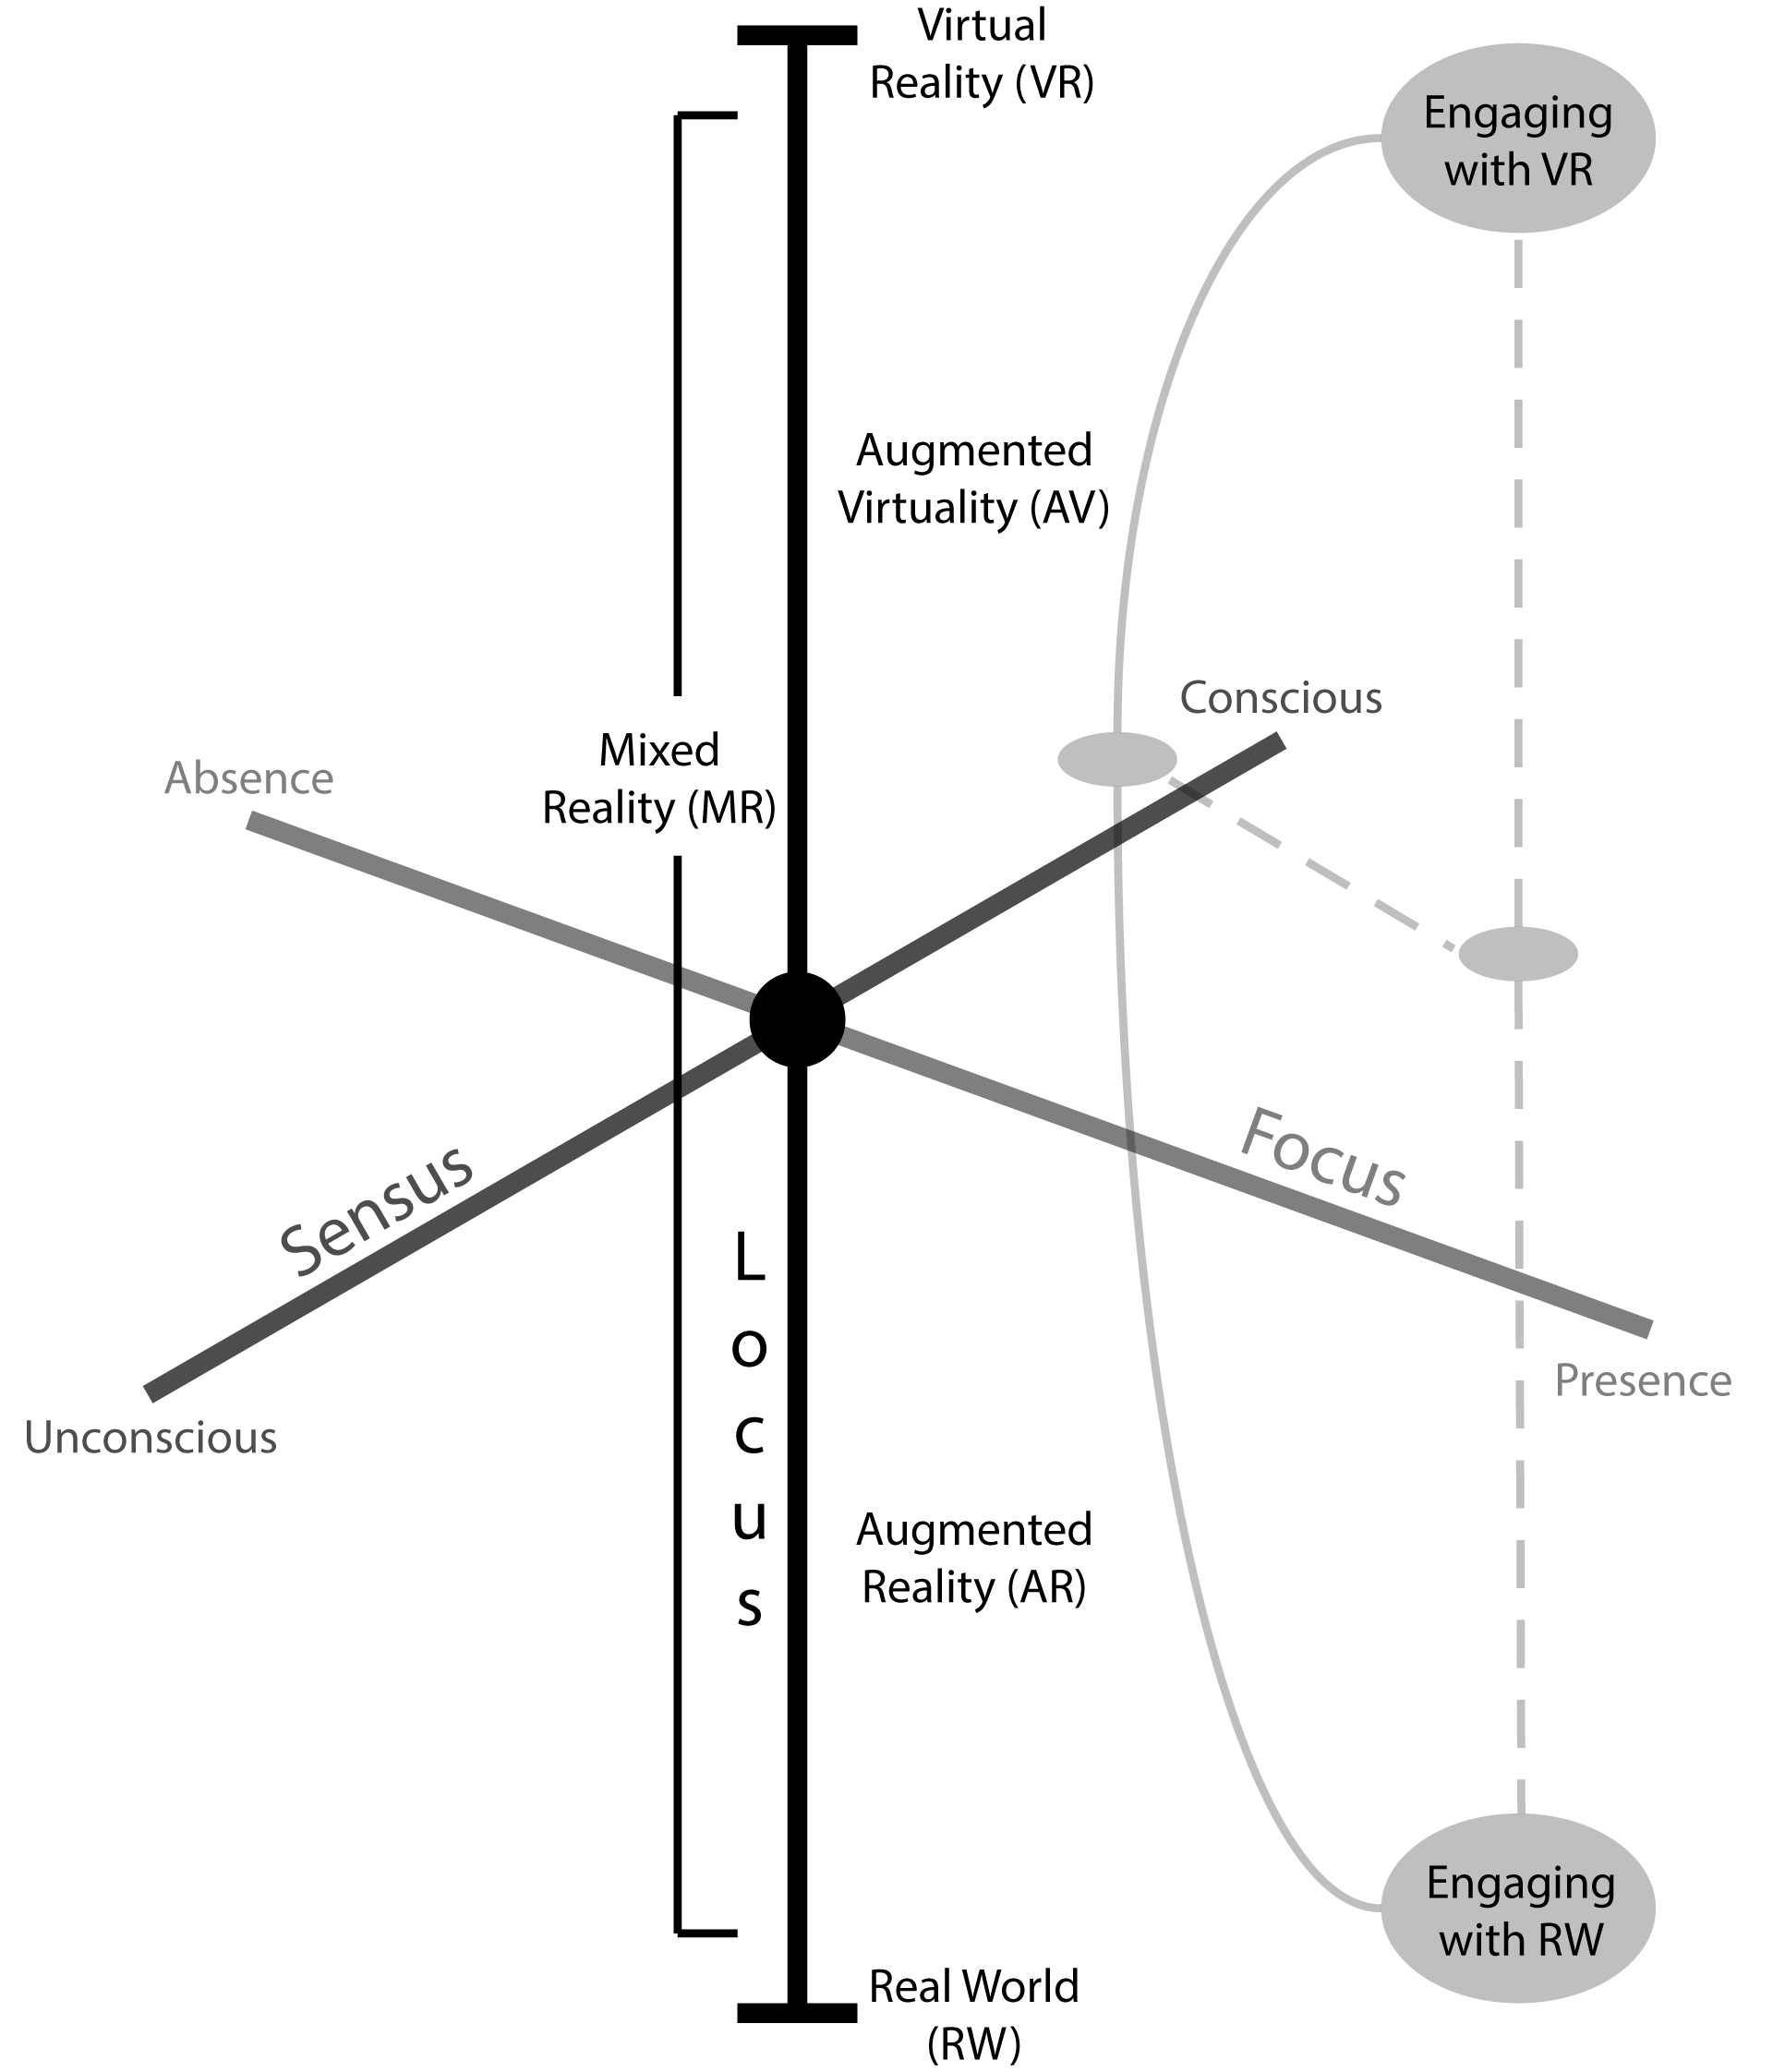
\includegraphics[width=0.7\textwidth]{focus-locus-sensus-with-virtuality-continuum-with-transition-updated.png}
		\caption{Operation of the Mirrorshades platform represented upon the combined model.}
		\label{focus-locus-sensus-with-virtuality-continuum-with-transition}
	\end{center}	
\end{figure}

%=========================================================================================================
%=========================================================================================================

\clearpage


%=========================================================================================================
%=========================================================================================================
%=========================================================================================================
%=========================================================================================================
%=========================================================================================================
%=========================================================================================================
%=========================================================================================================
%=========================================================================================================
%=========================================================================================================
%=========================================================================================================


Users are free to explore and interact with either environment in relative isolation from the other, even if their interactions in one trigger changes in the other, however simultaneous interaction and exploration with both environments has largely remained without systematic investigation.

This is largely because users exploring and interacting with the real environment do not have a convenient manner of also exploring and directly interacting with the virtual environment, as such interaction usually relies upon the use of software run on a desktop or laptop computer which is not conducive to mobile use. Using a laptop computer whilst walking around is far from convenient and using a desktop computer obviously limits the user's interaction with the real environment to that immediately around the location of the  computer and results in a disjoint relationship between their physical position in the real environment and the location of their avatar in the virtual environment when they navigate their avatar away from the respective position of their computer. This situation has been called `the vacancy problem'; an apparent vacancy from one environment whilst engrossed in the other.




%=========================================================================================================
%=========================================================================================================





%=========================================================================================================

Marie Kim et al at The Electronics and Telecommunications Research Institute, Korea, explain the cross reality paradigm well in terms of its principle features

\begin{quote}
\textit{``The important point of X-reality is a paradigm shift from single-directional information flows to bidirectional information flows between two worlds.''}
\end{quote}

and also how it can be employed for simultaneous presence in real and virtual environments

\begin{quote}
\textit{``The differential characteristic of X-reality is that it can augment user's engagement in the experiences of virtual presence and virtual world. Ultimately, it results in the human life span extension from the only real world to both worlds.''}
\end{quote}





Paradiso in IEEE Pervasive, Cross Reality Environments ~\cite{Paradiso2009} \textbf{***check this is the right citation***}

\begin{quote}
\textit{We call the ubiquitous mixed reality environment that comes from the fusion of these two technologies cross-reality. Sensor networks can tunnel dense real-world information into virtual worlds, where this data is interpreted and displayed to dispersed users. Interaction of virtual participants can incarnate into the physical world through a plenitude of diverse displays and actuators. We can envision a user's interface into this environment as an extension of human perception and interaction, augmenting our five senses well beyond the canonical ``here and now'' and redefining the meaning of presence.''}
\end{quote}



\begin{quote}
\textit{``We see cross-reality precipitating when diverse and ubiquitous sensor and actuator networks meet pervasively shared online virtual worlds, where phenomena freely tunnel between real and contrived continua at a multitude of ``wormholes'' opened by densely deployed networked devices, seamlessly adapting the level of immersion to match a variable ecology of available interfaces and user context or preference.''}~\cite{Lifton2009}
\end{quote}



%=========================================================================================================

\section{The Case for Mobile XR}

%ARCHEOGUIDE makes the point that AR is good because users are not isolated/completely immersed in a synthetic world - well Mirrorshades allows uers to more fully immerse themselves in a synthetic world, but without becoming isolated in it (eg without becoming ***vacant*** from the real world)

A XR system that presents the user with visual stimuli from both its constituent environments (RW \& VR) allows that user to engage with both real \& virtual content in a manner that is similar to, but has a number of advantages over, a traditional AR system;

\begin{itemize}
	\item the XR system is less critical of registration (the accurate positioning/alignment) between real \& virtual, as the virtual objects are seen as part of a larger virtual environment instead of being rendered atop a view of the real environment;
	\item the XR system can make use of existing VR content without the overhead of decanting/extracting a subset of the virtual components into an AR framework (e.g. manually selecting which objects within the VR environment are to be displayed over the RW environment);
	\item the use of a complete VR environment allows the virtual content to be more encompassing \& immersive, as presenting a complete VR environment allows total control over lighting, shadows, reflections, particle effects, etc. which would be difficult or impossible for an AR platform to render atop a view of a RW environment.
\end{itemize}

Thus, such a XR platform is well suited to situations in which interaction with both real \& virtual visual stimuli is required \& where one or more of the following hold true;

\begin{itemize}
	\item in lieu of accurate registration between real \& virtual, there is a strong focus on the virtual environment's atmosphere \& immersion~\cite{deamicis:gamebased};
	\item there is existing VR content;
	\item the visual differences between real \& virtual environments are so substantial that an AR system would resort to augment (\&/or diminish~\cite{Mann2002}) almost the whole RW view. While AR \textit{``smears an informational coating over real space''}~\cite{Andersen}, XR presents a complete, discrete virtual environment. AR is beneficial where one wishes the juxtaposition of virtual objects upon what is already present in the RW environment, however VR is better suited to situations where one wishes to present a complete virtual alternative.
\end{itemize}

%=========================================================================================================

% Original literature review from here on

Reviewing the literature on the domain of alternate realities this research finds that there is a gap in the scholarly investigation of simultaneous presence in real and virtual environments and the associated `vacancy problem'. This review proposes that a better understanding of the extension of human presence from only one of the real world or a virtual environment to simultaneous presence in both will permit the introduction of novel systems in a variety of fields in which simultaneous interaction and exploration of both real and virtual environments is possible. Such systems will likely be formed by expansion of research into \textit{cross reality}, an alternate reality comprised of complete real and virtual environments able to mutually reflect and influence each other via sensor/actuator infrastructure, and are likely to be in high demand as progress toward 3D extension of the Web continues.

\section{Conclusions}
We are rapidly approaching a situation in which ubiquitous sensor/actuator infrastructure allows us to access vast amounts of information about any location at any time and additionally to act upon this information and affect these locations. The continuing adoption of fast Internet connections, the increasing ability of commodity hardware including portable devices such as mobile phones and tablets to render complex three-dimensional graphics, and the development of 3D multi-user virtual environments that place an emphasis on notions of community, creation and commerce instead of competitive gaming, all point toward a continuing natural progression toward 3D extension of the Web on a large scale.

It is already common to see people spending substantial amounts of time immersed in the 2D textual/graphical Web whilst simultaneously interacting with the real world around them. This desire to maintain a Web presence whilst simultaneously interacting with the real world is set to remain as interaction with the Web evolves from 2D to 3D. Thus it is prudent to investigate approaches for implementing and applications for exploiting the concept of simultaneous presence in real and virtual 3D environments, whether spatially equivalent or not.

This review has unearthed a plenitude of research on numerous alternate realities, either experienced in isolation from other realities (reality, virtual reality) or by mixing limited amounts of one with another (augmented reality, augmented virtuality) however has discovered a comparative lack of research attention focussed on the concept of simultaneous presence and interaction with two complete environments, one real and the other virtual. Cross reality is the closest existing concept, however the vast majority of the research in this field has used statically located computers to access the virtual environments, preventing users from exploring or interacting with the real environment that is not immediately surrounding them; the true notion of simultaneous presence in real and virtual environments requires freedom of movement and interaction with both environments, perhaps by adopting a manner of interaction with the virtual environment similar to that of the VTW project.

This deficiency of research into simultaneous presence in real and virtual environments warrants addressing with further academic investigation, as it represents a style of interaction that is bound to become commonplace as progress toward 3D extension of the Web continues at an accelerated pace.


% ======= ======= ======= ======= ======= ======= =======

\chapter{A Virtual Time Window}
\graphicspath{ {04_vtw/images/} }
\begin{quote}
	\textit{``The sinister thing about a simstim construct, really, was that it carried the suggestion that any environment might be unreal, that the windows of the shopfronts she passed now with Andrea might be figments.''}
\end{quote}
\hfill \textit{Count Zero, William Gibson}
\\
\\

%=========================================================================================================
%=========================================================================================================

\label{chapter-vtw}

This chapter presents the development of a preliminary PR system that combined a tablet computer, GPS, accelerometer \& magnetometer, with an OpenSim based virtual environment to allow exploration of the real world ruins of a 14th century cathedral with a virtual reconstruction of it as it stood in its prime. Cultural heritage is introduced as an ideal area for which PR systems can be applied to beneficial effect, while the accuracy of GPS tracking emerged as a constraint on this style of implementation.

%=========================================================================================================

\section{Virtual Heritage}

Alternate reality technologies have been used for over two decades~\cite{Roussou2002} to aid in the investigation, understanding \& dissemination of information pertaining to our past in the fields of archaeology \& cultural heritage. Whilst archaeology studies human activity through the recovery of remains, heritage is also concerned with intangible attributes of society; tradition, art, narratives \& other cultural evidences~\cite{Roussou2002}. \textit{Virtual heritage} is the name given to the application of advanced imaging techniques, including alternate reality techniques, to the synthesis, conservation, reproduction, representation, reprocessing \& display of this cultural evidence~\cite{roussou:photorealism}.

These techniques provide access to locations \& artefacts scattered about the world, that may reside in private collections inaccessible to scholars (much less interested amateurs) \& outwith of their original context of creation~\cite{griffin:recovering}. They allow recreations to be made of the numerous cultural heritage objects that are deteriorating or are at risk of being lost, both due to natural causes such as weather \& natural disasters but also due to acts of man such as civil war~\cite{Ikeuchi2003}.

Virtual heritage techniques offer substantial benefits to collaborative investigation of sites, where multiple users are provided the ability to collaborate via a multitude of different visualization modalities including video see-through head-tracked head mounted displays, projected table surfaces, large screen displays \& tracked hand-held displays, including the ability for experts physically located at a particular site to collaborate with those remote to it~\cite{benko:collaborative}. This combination of different techniques not only benefits experts, but has been used in the creation of contiguous platforms for building \& managing exhibitions of 3D models of artefacts accessed in museums, galleries \& via the Web~\cite{Wojciechowski2004}, focussed not only on the digitization \& subsequent interaction with such content to aid in its preservation \& protection, but also with making these resources as widely available as possible to any interested parties (scientists, archaeologists, curators, historians \& interested amateurs)~\cite{walczak:applications}.

Even traditionally two-dimensional visual resources associated with cultural heritage can be integrated into such state-of-the-art systems, visualized via immersive CAVE techniques as part of `information landscapes'~\cite{Ruffaldi2008}. Such techniques are of particular benefit to young people as cultural heritage sites often arouse little involvement in them, especially if the site's present day appearance bears few traces of its original stature \& makes it difficult to appreciate its original splendour \& importance~\cite{ardito:combining}.

%=========================================================================================================

\subsection{Alternate Reality Techniques in Virtual Heritage}

Due to the number of combinations \& diversity in approaches that have been used in the application of visualization techniques to the cultural heritage sector, attempting to comprehensively list them is impractical. Comparison via a taxonomical model that classifies approaches according to various characteristics is thus the approach adopted by Foni et al.~\cite{Foni2010} that produced the taxonomical space shown by figure \ref{taxonomy_1.png}.

\begin{figure}[h]
\centering
  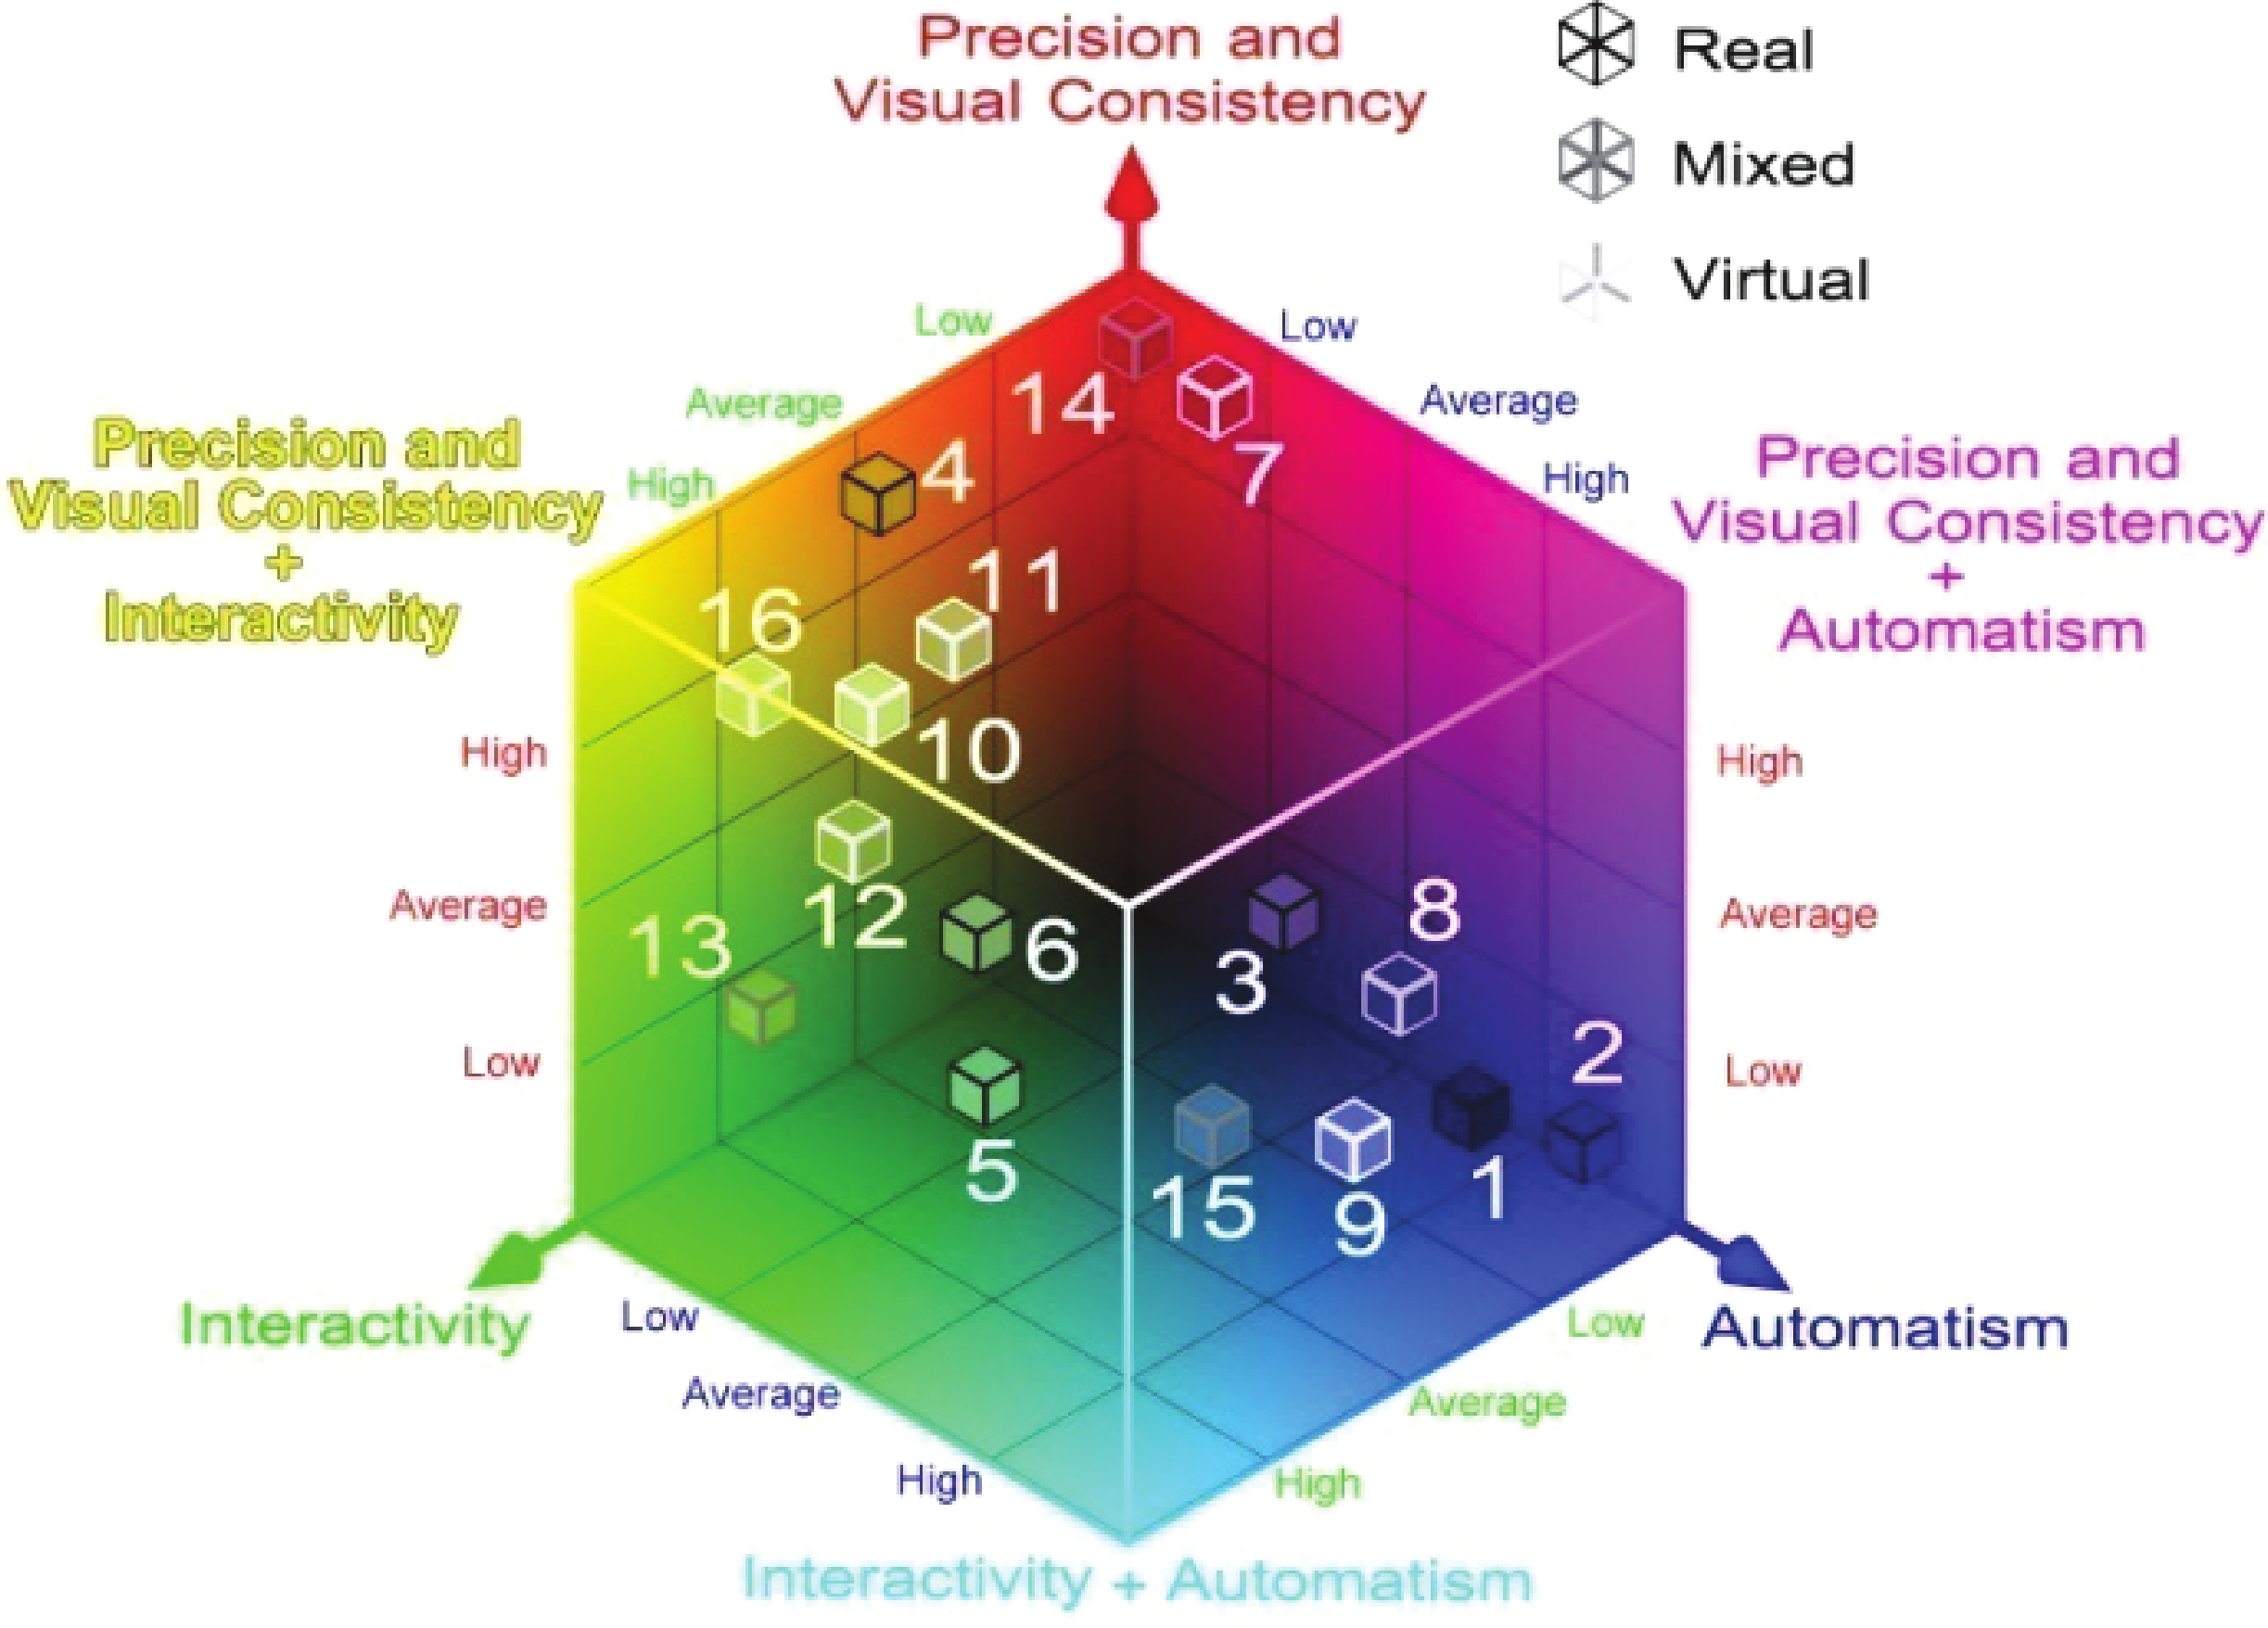
\includegraphics[width=.7\linewidth]{taxonomy_1.png}
  \caption{Taxonomical space of visualization strategies used in cultural heritage.}
  \label{taxonomy_1.png}
\end{figure}

This model classifies visualization strategies according to four continua, represented by the three physical dimensions of the 3D cube \& the degree of shading of each point within the cube. The x axis represents the level of automatism, which refers to the span of the development cycle required to produce the visualization; the y axis represents the level of precision, referring not only to the amount of geometrical detail but to all elements that can contribute to or enhance reliability; \& the z axis represents the level of interactivity, defined in this context as;

\begin{quote}
	\textit{``its capacity to contextually offer the possibility to subjectively experience an interactive behaviour in a synchronous way, thus enabling the user the opportunity to meaningfully contribute to a given experience or to affect in real time the visualized  item''}~\cite{Foni2010}.
\end{quote}

The shading of each point within the cube represents its degree of virtuality, conceptually analogous to the reality-virtuality continuum of Milgram et al. (see section \ref{milgram&kishino}) with real world/world unmodelled represented as solid black, virtual reality/world completely modelled as completely white \& positions in-between as various shades of grey. The position of 16 exemplar visualization techniques applied to cultural heritage are shown upon the cube \& explained via the table figure \ref{taxonomy_2.png}, which includes both traditional techniques \& state-of-the-art methodologies.

\begin{figure}[h]
\centering
  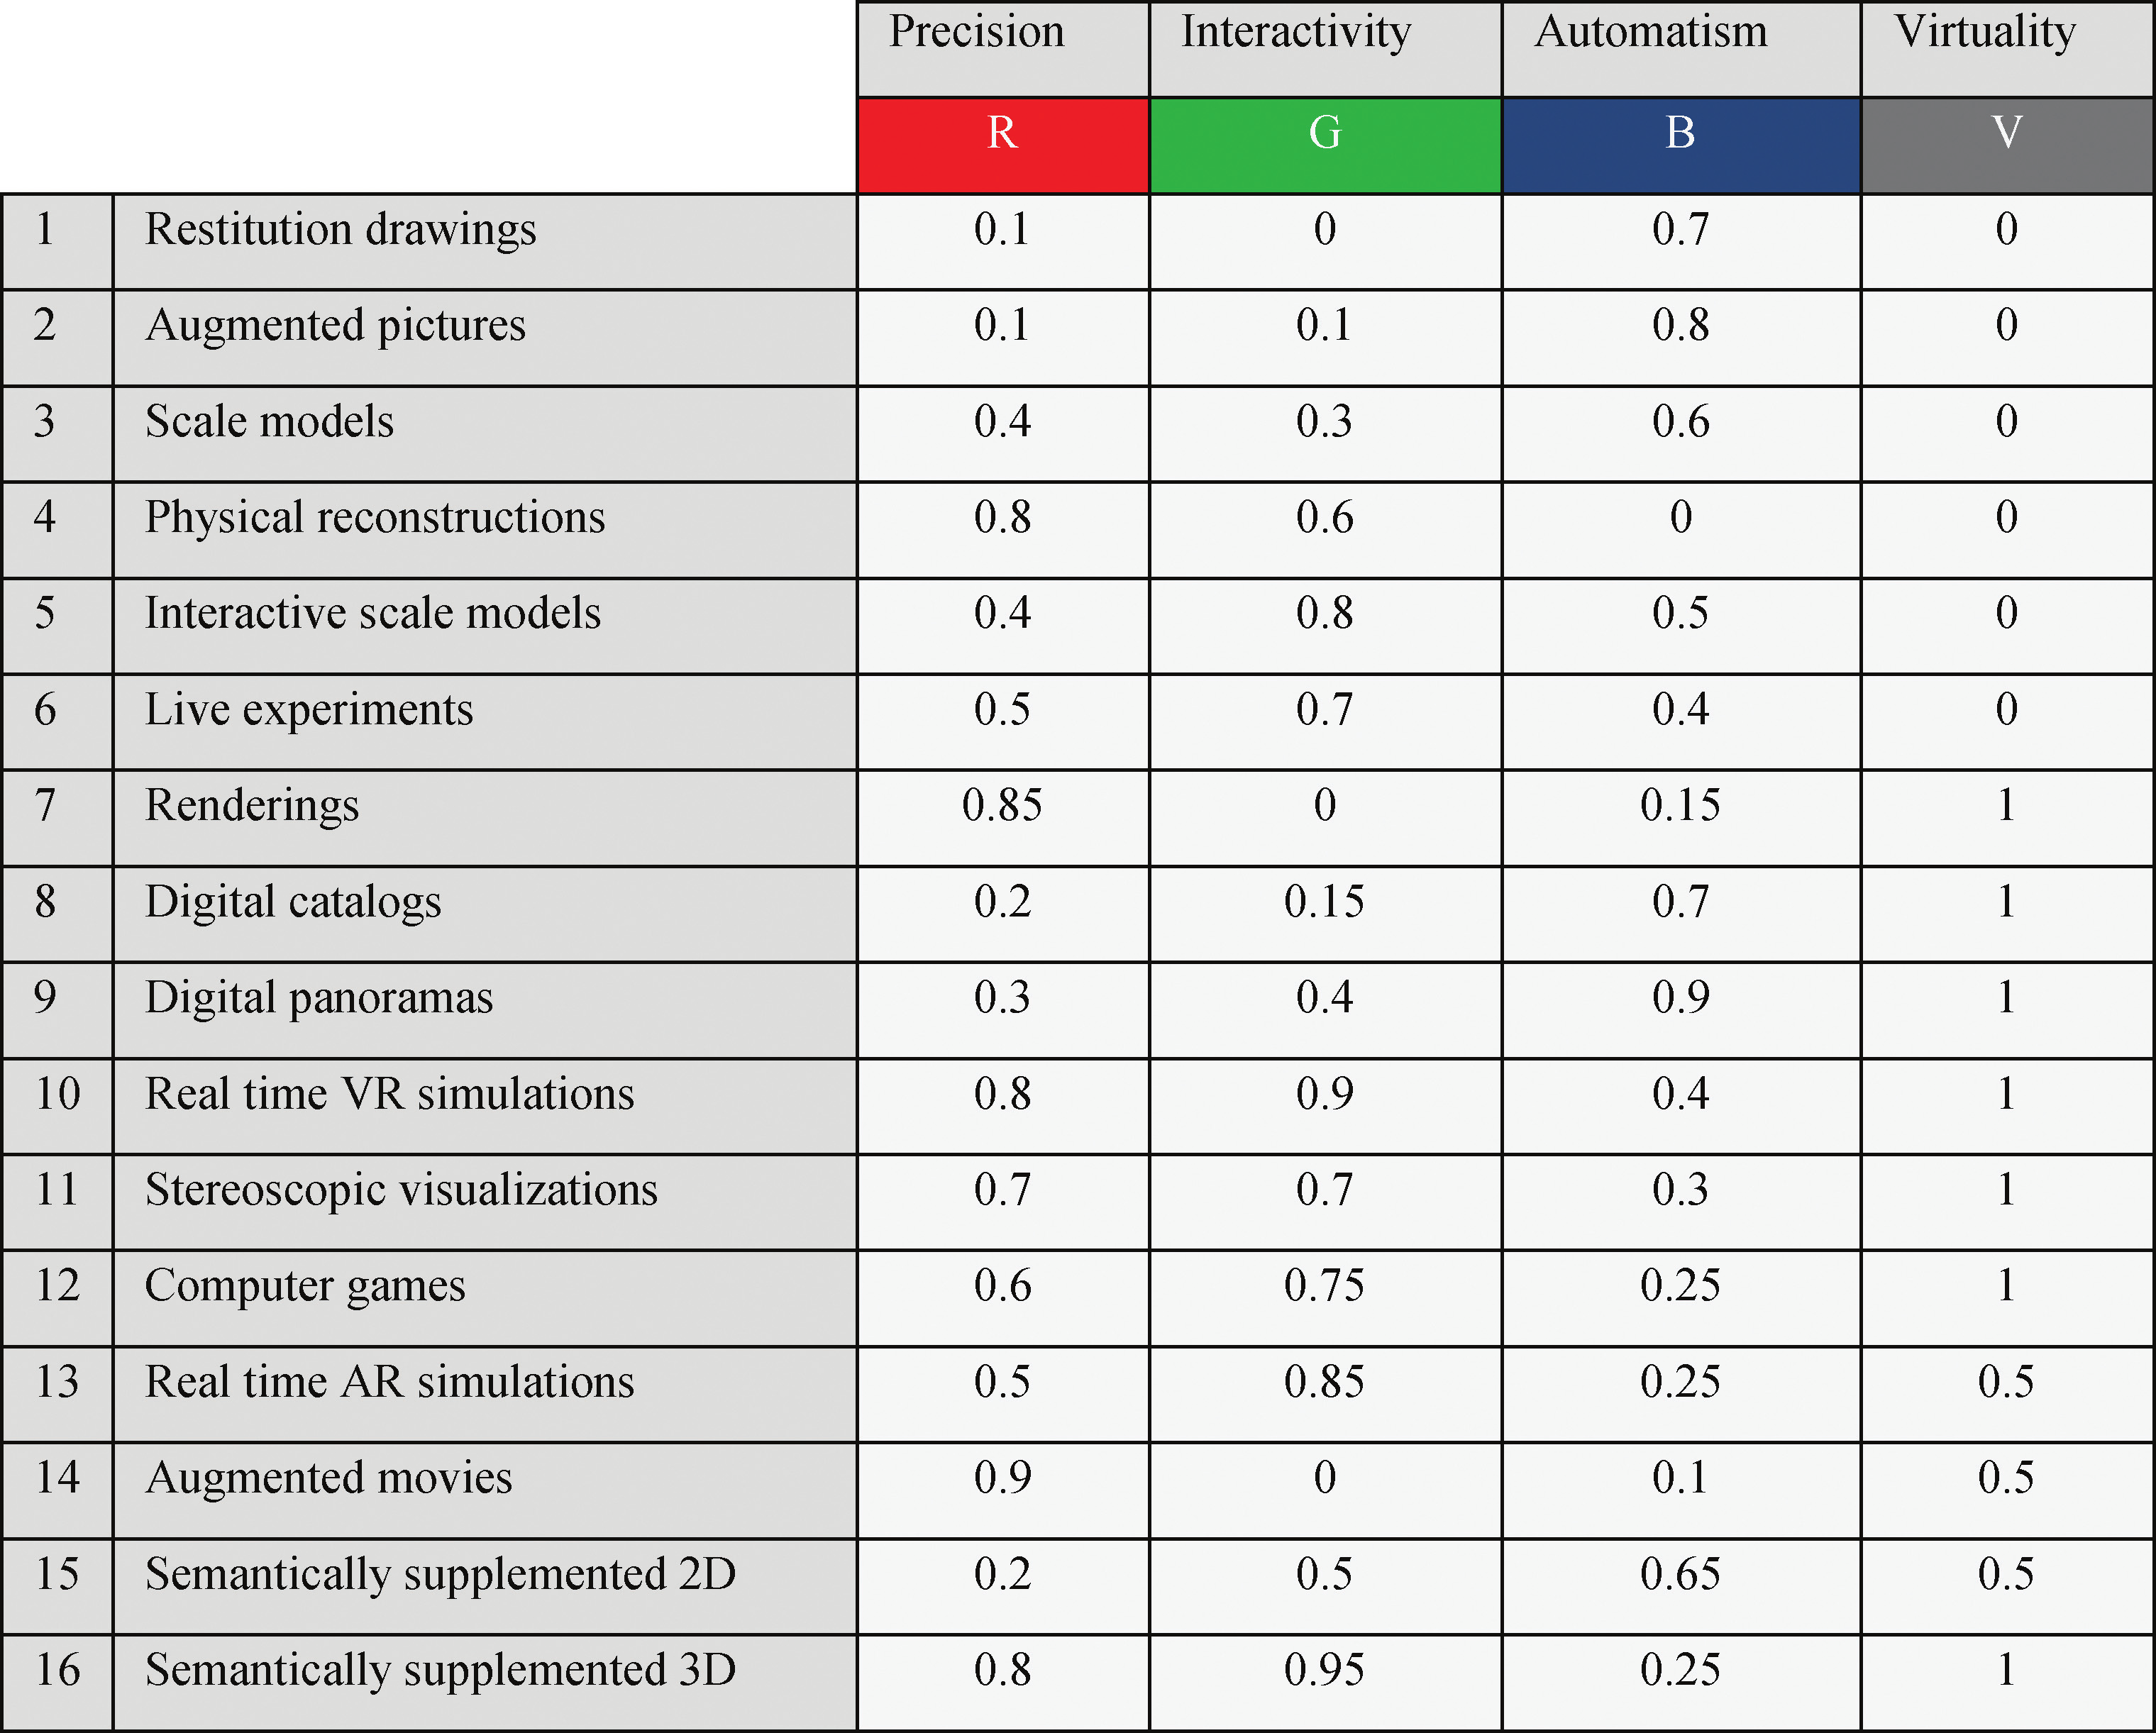
\includegraphics[width=.8\linewidth]{taxonomy_2.png}
  \caption{Coordinate sets for each approach within the taxonomical space (figure \ref{taxonomy_1.png}).}
  \label{taxonomy_2.png}
\end{figure}

%=========================================================================================================

In terms of alternate reality techniques, real time AR simulations (category 13) have been used to add artefacts, actors \& reconstructed architecture to views of present day sites that are still accessible \& may bear traces of their original status, whilst real time VR simulations (category 10) have been used to host more complete reconstructions of entire buildings \& settlements for interaction via screen, HMD \& CAVE, including where the present day site bears no evidence of its past status or is inaccessible due to latter development, change in landscape, etc..

%=========================================================================================================

The ARCHEOGUIDE project (Augmented Reality-based Cultural Heritage On-site GUIDE)~\cite{vlahakis:archeoguide} aimed to provide a `personalized electronic guide \& tour assistant' to cultural heritage site visitors. On-site help \& augmented reality reconstructions of on-site ruins were presented via a laptop, a tablet computer \& a PDA, using GPS for location tracking \& magnetometer to ascertain direction such that augmentations could be placed accordingly. The applications claimed to be supported by the platform range from archaeological research to education, multimedia publishing \& cultural tourism. The platform was prototyped at the archaeological site of Olympia, Greece.

As well as being used for walking tours, AR has been combined with the concept of telepresence to create `augmented telepresence', allowing participants to experience a `fly-through' of the ancient Nara Heijo-kyo capital of Japan, by combining aerially captured omnidirectional video augmented with related information using AR techniques~\cite{Okura2006,Okura2011}.

Augmenting views of the real world with real-time animated virtual humans has been explored by several projects, including the LIFEPLUS EU IST project, which aimed to produce `\textit{`an innovative 3D reconstruction of ancient frescos-paintings through the real-time revival of their fauna and flora, featuring groups of virtual animated characters with artificial life dramaturgical behaviors, in an immersive AR environment''}. This project pushed established augmented reality applications to the field by exploring narrative design in fictional spaces, with the aim of increasing immersion via realistic interaction, making use of captured/real-time video of a real scene~\cite{Papagiannakis2004}, presenting the visitor with \textit{``an immersive and innovative multi-sensory interactive trip to the past''}~\cite{Papagiannakis2005}. These realistic simulations of animated virtual human actors were employed in a mobile \& wearable setup, in abandonment of traditional concepts of static cultural artefacts or rigid augmentations of real world features, making use of a markerless camera tracker \& mixed reality illumination model for more consistent real-virtual \& virtual-real rendering. This platform was demonstrated in a case study on the real site of ancient Pompeii \& whilst initially targeted at the cultural heritage sector, the author(s) clarifies that as a platform it is not limited to such subjects~\cite{Papagiannakis2007}. This concept of extending rigid \& static AR with character-based event representations hopes to recreate not just discrete artefacts but the entirety of `daily life' at the scene~\cite{Papagiannakis2009}.

Although many applications of AR to cultural heritage sites are mobile in nature, using a variety of tracking techniques to localise the user \& determine their orientation, including GPS~\cite{vlahakis:archeoguide}, visual tracking of robust features of the environment~\cite{Kim2009} \& omnidirectional range sensing of a landmark database~\cite{Taketomi2011}, there are also those that present a static interface similar to coin-operated telescopes situated at popular tourist attractions~\cite{Weng2012}.

%=========================================================================================================

VR is not only useful where the real site is no longer accessible, too remote or does not bear any similarity to its original status, but also allows for more effective control over the atmospheric qualities of the environment being recreated; effects such as fog, sky, water \& particles, exploiting the latest graphical hardware by making use of shaders to deliver high quality graphics~\cite{deamicis:gamebased}. The use of a head mounted display or CAVE~\cite{cabral:x3dexperience,Christou2006} that completely blocks stimuli from the user's real world surroundings allows for this complete level of control. Unless an AR system employs various environmental monitoring techniques, the augmentations that it overlays upon the user's view of the real world will often have differing illumination than their real surroundings which has an effect upon their perceived realism~\cite{mcnamara:lightness}.

Whereas many heritage representations, architectural walkthroughs \& simulations of artefacts \& places have defined a practice where photorealism is considered an important measure of the representation's success, there is an argument that whilst such an emphasis on realism \& historical accuracy \& authenticity is important, such photorealistic methods can limit the flexibility of the reconstructions with regards to how much they can be modified \& altered to explore different reconstruction hypotheses~\cite{roussou:photorealism}. Emphasis on photorealistic graphical quality also has considerations when it comes to real time performance \& many intelligent techniques must be employed to maintain acceptable performance as complexity of reconstructions increases~\cite{willmott:largecomplex}. Particularly for dissemination to the public in museums \& visitor centres, acceptable performance is often more important than extreme historical accuracy.

%=========================================================================================================

\subsection{Virtual Heritage at the University of St Andrews}

\label{virtual-heritage-at-st-andrews}

\textbf{***Include references to Kris Getchell's thesis? Experiential learning, etc?}

The Open Virtual Worlds (OVW) research group at the School of Computer Science at the University of St Andrews has been employed in virtual heritage projects since 2007~\cite{Getchell2007}, producing a number of reconstructions of cultural heritage sites in Scotland \& further afield. These reconstructions have been produced through collaborations with academics from the university's Art History, History \& Archaeology departments, as well as with domain experts from heritage organisations including Historic Scotland \& the National Trust for Scotland. These projects range from small reconstructions of a church, to much larger reconstructions such as that of the cathedral at St Andrews which represents several years of work~\cite{Kennedy2013}. Whilst the cathedral reconstruction was completed as a research project, other reconstructions were produced specifically for use in schools in Scotland (such as Linlithgow palace, figure \ref{linlithgow_real.jpg}, \ref{linlithgow_reconstruction.png}), others for outreach purposes (Mosfell Viking farmstead, figure \ref{mosfell_outside.jpg}, \ref{mosfell_inside.jpg}) \& still others were built specifically for installation into museums (Caen Township, figure \ref{caen_township_outside.jpg}, \ref{caen_township_inside_wireframe.jpg}). Some of these reconstructions are inhabited with virtual humans that are scripted to perform certain actions specific to the role they depict at the site (figure \ref{cathedral_npc_standing.png}, \ref{cathedral_npc_talking.png}).

\TwoFig{linlithgow_real.jpg} {Linlithgow Palace today.} {linlithgow_real.jpg}
       {linlithgow_reconstruction.png} {Linlithgow Palace reconstruction.} {linlithgow_reconstruction.png}

\TwoFig{mosfell_outside.jpg} {Mosfell Viking Longhouse.} {mosfell_outside.jpg}
	   {mosfell_inside.jpg} {Longhouse interior.} {mosfell_inside.jpg}

\TwoFig{caen_township_outside.jpg} {Caen Township.} {caen_township_outside.jpg}
       {caen_township_inside_wireframe.jpg} {Caen Township wireframe detail.} {caen_township_inside_wireframe.jpg}

\TwoFig{cathedral_npc_standing.png} {Virtual humans in cathedral reconstruction.} {cathedral_npc_standing.png}
       {cathedral_npc_talking.png} {Conversing with virtual humans.} {cathedral_npc_talking.png}

These reconstructions were made using OpenSim, an open source implementation \& extension of the Second Life server which is compatible with the numerous forks of the Second Life client program. This architecture allows straightforward construction \& dissemination of the models, thanks to accessible modelling tools provided by the Second Life client itself \& the client/server model that allows the models to be accessed in various deployment scenarios including temporary deployments within controlled network \& client conditions as well as remotely via the Internet.

The reconstruction process involves the use of Geographic Information System (GIS) data from Ordnance Survey (OS) to accurately model the basic elevation of the ground. Where there is higher resolution elevation data, such as from Lidar laser surveying often employed on archaeological surveys, this is used to increase the accuracy of the resultant reconstruction. Where access to the site is possible \& depending upon development surrounding the site prior to the date being reconstructed, 360\textdegree\ panoramic photographs are captured \& then used to create a backdrop for the reconstruction, allowing identifiable aspects of the surrounding environment to improve the experience of the reconstruction. Buildings/structures are then reconstructed upon the ground layer, using numerous sources as input; satellite views, archaeological surveys, contemporary accounts, views of the site itself if relics still exist, photographic evidence, etc. Domain experts are then brought in to iteratively improve the model, commenting on aspects of the reconstruction to be altered in order to visualise a different reconstructive hypothesis.

These reconstructions have been used to host workshops at 10 schools throughout Scotland, at both primary \& secondary institutions, where all requisite computing infrastructure was taken, assembled at the school, then disassembled \& removed at the end of the day. Students are split into groups of 4-5, sharing a computer with screen, keyboard, mouse \& Xbox controller (a control modality instantly recognised by most school students). Worksheets with tasks are used to structure their interaction with the reconstructions \& guide the experiential learning experience over 20-40 minute sessions (figure \ref{linlithgow_children.jpg}). Similar workshops have also been performed in museums, using the same approach of temporary setups of computing hardware (figure \ref{musa.jpg}). In addition to traditional computer screens, larger LCD television screens \& still larger projection screens, Oculus Rift VR headsets have been used with this same content~\ref{rift_exhibition.jpg}.

In addition to these temporary workshops, the reconstructions have also been used in permanently installed exhibits in museums \& visitor centres, including the Virtual Time Travel Project (VTTP), which combines multi-head projection with Natural User Interaction (NUI) via Microsoft Kinect, which has been installed at the Timespan Museum \& Arts Centre in Helmsdale, allowing visitors to explore the reconstruction of the Caen Township by using simple gestures, instead of relying upon a keyboard, game controller or other traditional interface (figure \ref{VTTP_projection.png}).

\TwoFig{linlithgow_children.jpg} {School students learning via a reconstruction.} {linlithgow_children.jpg}
       {VTTP_projection.png} {VTTP installation at Timespan.} {VTTP_projection.png}

\TwoFig{rift_exhibition.jpg} {OVW via Oculus Rift.} {rift_exhibition.jpg}
       {musa.jpg} {Museum workshop.} {musa.jpg}

%=========================================================================================================

\subsection{Parallel Reality in Virtual Heritage}
Applications of alternate reality techniques within virtual heritage have thus far broadly fallen into the categories of AR, experienced at the site, or VR, experienced away from the site (in terms of space, time, or both). The dissemination of the OVW group's content has been no exception to this observation, falling into categories 10-12 of figure \ref{taxonomy_2.png}, with complete virtual environments that are experienced with both spatial \& temporal separation from the real site that they represent.

Applying the concept of parallel reality to virtual heritage represents an opportunity to explore an exciting new modality of interaction that combines the complete virtual environments of categories 10-12 with the real time juxtaposition between real \& virtual environments of AR systems from category 13. In terms of the four categories of the taxonomic space, such a PR system would combine the high precision \& interactivity of a VR system (category 10) with two values of viruality, as the user is provided the ability to observe either the complete virtual environment (virtuality = 1) or the unmodified real environment (virtuality = 0). The automatism of such a system would occupy a position between that of VR \& AR; whilst the system will require a more involved development cycle than a purely VR one, the slackened requirements on registrational accuracy of a PR system compared to an AR system promise higher automatism than a purely AR system.

%=========================================================================================================

\section{The Virtual Time Window}
The Virtual Time Window (VTW) is an application of parallel reality to virtual heritage, leveraging the OVW group's existing OpenSim virtual reconstructions of cultural heritage sites in a handheld package that allows tandem exploration of both the real cultural heritage sites \& their spatially equivalent virtual reconstructions.

VTW manifests as a tablet computer which is capable of tracking its position via GPS, its compass heading via magnetometer (`electronic compass') \& its pitch via accelerometer. Existing AR projects have proven through application the suitability of smartphones \& tablets for mobile, position \& orientation aware applications that present virtual content within a cultural heritage context. These devices are also entering ubiquity today \& thus present a platform that can be quickly assimilated by most users. The tablet runs a modified version of the Second Life client in order to access, via wifi, a virtual reconstruction of a cultural heritage site hosted by an OpenSim server. The Second Life client is controlled entirely by the tablet's position \& orientation - the user does not manually control any aspect. The modality of interaction offered is similar to that of using a smartphone to take a photograph, but whereas the screen of the smartphone shows the real environment as it is, the screen of the VTW tablet shows the environment as it was in the past - a window to the past, or \textit{Virtual Time Window}. The user is free to explore the real cultural heritage site, observing it in its current state, whilst at any moment `looking through' VTW to see what a particular vantage looked like in the past. See figure \ref{vtw_high_level.png} for a representation of the components of the platform at the conceptual level.

\begin{figure}[h]
\centering
  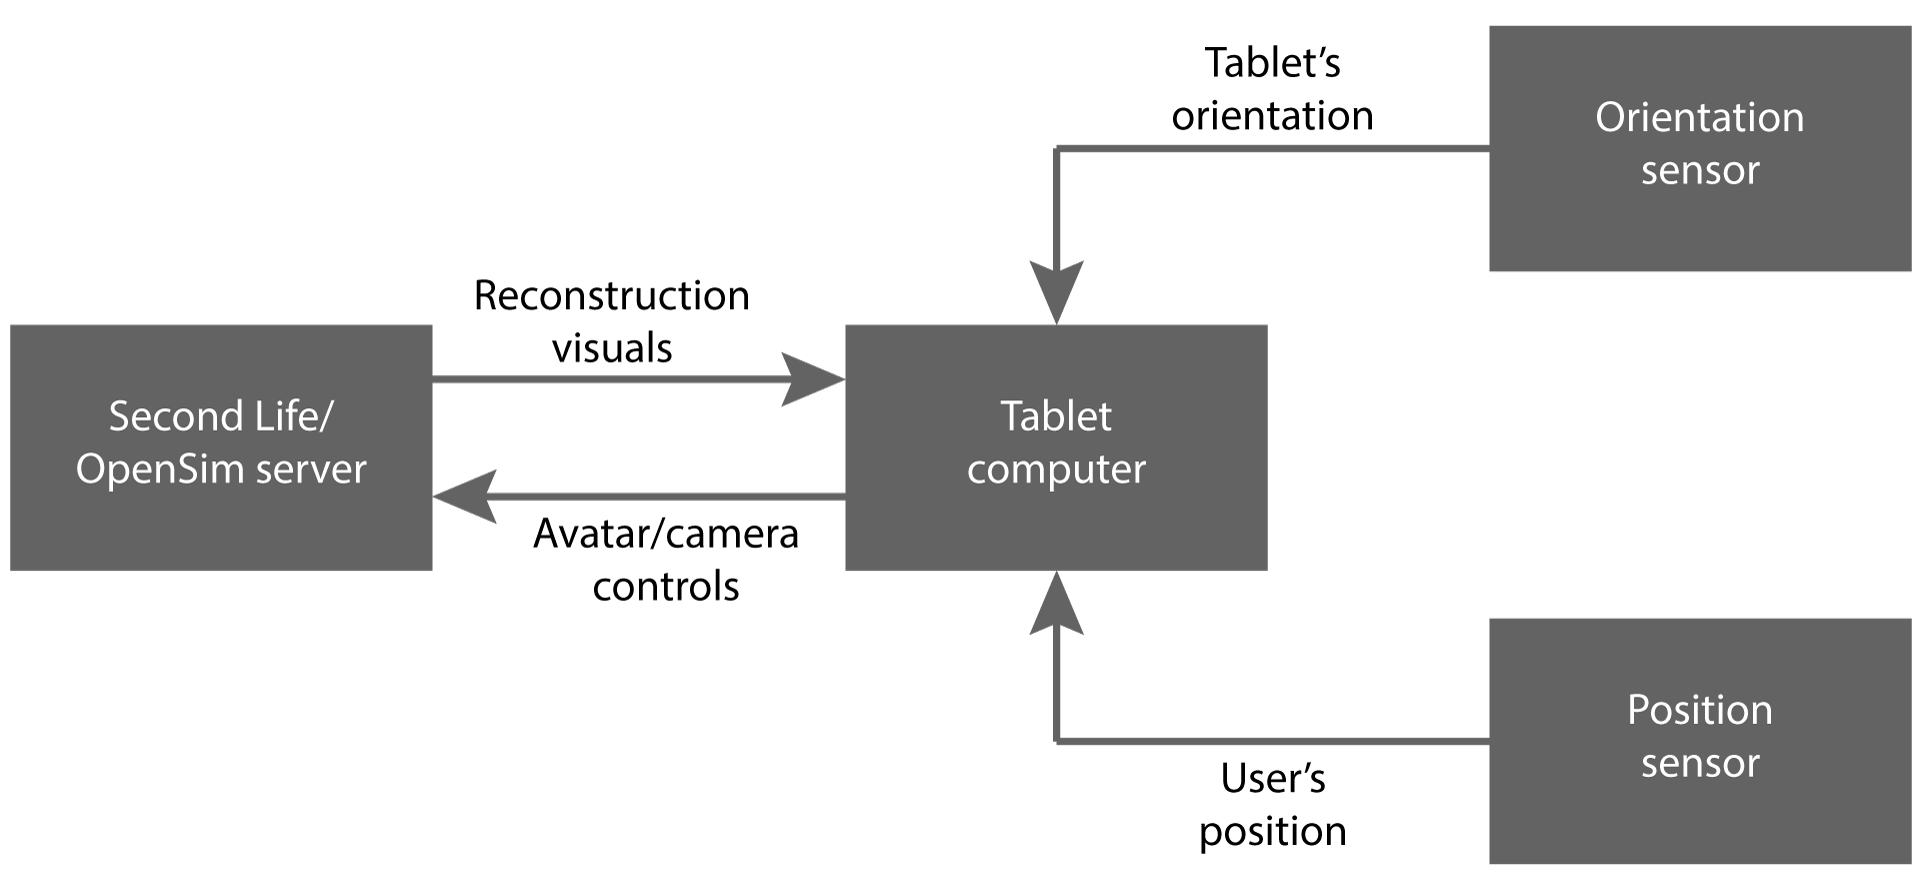
\includegraphics[width=.7\linewidth]{vtw_high_level.png}
  \caption{High level architecture of VTW.}
  \label{vtw_high_level.png}
\end{figure}

In terms of the combined Milgram/Waterworth model, the displacement along the locus axis when the user switches their attention between their real environment \& the virtual environment upon the tablet will displace less toward the VR extremum than shown in figure \ref{focus-locus-sensus-with-virtuality-continuum-with-transition} which represents transitions between real \& virtual environments when using a HMD that effectively blocks all stimuli from the real world when observing the virtual. When considering the environmental provision, VTW features two complete environments, one real \& the other virtual. From the perspective of transitioning between receiving stimuli from each environment, there is an obvious difference between VTW's tablet based approach compared to a HMD approach, as the latter effectively forces all percepts to emanate from one environment whilst the former allows percepts emanating from both environments to be perceived simultaneously.

Whilst this will intuitively make transitions easier to perform \& create less risk of a jarring Gestalt switch, it will also intuitively limit the intensity of the sense of presence attainable in the virtual environment as the sense of `looking in to' the virtual environment will always leave the user readily aware of the real environment surrounding them. Whilst VTW is a PR system, one might liken the experience of interacting with it to be similar to that of an AR system.

%Map showing spatial separation of Madras \& cathedral?

%How with VTW we have a small `window' into the virtual, which is then surrounded by the real. So unlike Mirrorshades which is about distributing attention by time (one environment, then the other), VTW is about distributing attention by gaze/place (different parts of a single view/combined environment).

%=========================================================================================================

\subsection{Second Life \& Mobility}

\label{SecondLifeMobility}

\newcommand{\LumiyaFootnote}{\footnote{\url{https://play.google.com/store/apps/details?id=com.lumiyaviewer.lumiya&hl=en_GB}}}

\newcommand{\WindpadFootnote}{\footnote{\url{http://www.msi.com/product/windpad/WindPad-110W.html}}}

%=====================

At the time of the VTW project (Summer 2012) the only fully-featured Second Life clients available were for x86 platforms. Whilst the Android client Lumiya\LumiyaFootnote{} was available, it was in its earliest stages \& very limited in its features \& usability. This limited the choice of tablet to those few x86 models that had reached market, with the MSI WindPad 110W\WindpadFootnote{} presenting the most promising solution: a 10'' tablet sporting an AMD Brazos Z01 APU (combining a dual-core x86 CPU with a Radeon HD6250 GPU).

The Second Life client, intended for use on a desktop or laptop computer, provides provision for controlling the avatar's position \& the camera orientation by keyboard, mouse \& joystick. For the purposes of VTW, this position \& orientation control must be tied to the physical position \& orientation of the tablet itself. To this end, it is necessary to make use of various sensors connected to the tablet (either internally, or externally) \& to interface these with the Second Life client in such a way that it can make use of their collected data to appropriately control the avatar's position \& camera orientation.

%\cite{willmott:largecomplex} occlusion culling etc., missing in Second Life/OpenSim

%Talk about history of Second Life/OpenSim in academia/research, including original cross reality research.

%The 3D virtual environment component of the Pangolin system was implemented using the Second Life/OpenSimulator (SL/OpenSim) platform, which provides a 3D social-oriented multi-user non-competitive virtual environment which focuses on the community, creation and commerce~\cite{Sevan2008} aspects of many users interacting within a shared space through the abstraction of avatars, rather than the competitive natures of games and the solitary environments commonly afforded by simulation and visualization platforms.

%The distributed client/server model of SL/OpenSim, wherein 3D content is stored on a grid of servers operated by a multitude of organizations and distributed to and navigated between by dispersed clients on demand when they enter a particular region rather than being pre-distributed as is the norm for games, simulations and visualizations, is analogous to the manner in which 2D social Web content is served from Web servers to client browsers and apps.

%This style of content delivery is necessary when considering the dynamic and ephemeral nature of consumer-generated media which constitutes the majority of the current 2D social Web and will make up the majority of expanding 3D social Web content.

%=========================================================================================================

\section{Orientation Control}

\label{OrientationControl}

\newcommand{\ArduinoFootnote}{\footnote{\url{http://www.arduino.cc/}}}

\newcommand{\MMAfootnote}{\footnote{\url{http://cache.freescale.com/files/sensors/doc/data_sheet/MMA8452Q.pdf}}}

\newcommand{\ADXLfootnote}{\footnote{\url{http://www.analog.com/static/imported-files/data_sheets/ADXL335.pdf}}}

\newcommand{\HMCfootnote}{\footnote{\url{http://www51.honeywell.com/aero/common/documents/myaerospacecatalog-documents/Defense_Brochures-documents/HMC5883L_3-Axis_Digital_Compass_IC.pdf}}}

\newcommand{\HMCtwoFootnote}{\footnote{\url{http://www51.honeywell.com/aero/common/documents/myaerospacecatalog-documents/Missiles-Munitions/HMC6343.pdf}}}

\newcommand{\HMCvccFootnote}{\footnote{The HMC6343 requires 2.7 to 3.6V input on VCC/VDD, this table showing connection to 5V assumes a HMC6343 breakout with appropriate step down.}}

\newcommand{\itwocFootnote}{\footnote{The HMC6343's I2C lines must be pulled up to 3.3V, this table shows connection to an Arduino Uno R3's I2C lines which are pulled up to 5V assuming a HMC6343 breakout with appropriate level shifters.}}

%http://www.nxp.com/documents/user_manual/UM10204.pdf

%=====================

In order to control Second Life's camera in the fashion required of VTW, sensor data are required for the orientation in which the user is holding the tablet. Specifically, the tablet's yaw \& pitch are needed; roll is less important as it is conceived that the user will generally hold the tablet roughly level with the horizon when looking `through' it.

VTW considers yaw in terms of magnetic compass bearing, as this provides a value that can be used to directly control the yaw of the virtual camera while the virtual reconstruction within OpenSim is correctly oriented to OpenSim's own compass. Magnetic compass bearings are sensed electronically via a 3-axis microelectromechanical (MEMS) magnetometer, which measures the strength of magnetic field being experienced along each of its 3 axes. By comparing the values of each axis to the known direction of the field lines of Earth's magnetic field, a compass bearing relative to the magnetometer's orientation can be calculated. Pitch is sensed using a 3-axis MEMS accelerometer, which measures force of acceleration along each of its 3 axes. In the case of static or slow moving applications, this acceleration is predominantly that caused by the Earth's gravitational pull \& by comparing the values of each axis the direction of this acceleration (down toward the centre of the Earth) can be determined in relation to the orientation of the accelerometer itself \& thus the accelerometer's own orientation can be deduced.

Due to the fact that the WindPad tablet does not feature a built-in magnetometer \& its built-in accelerometer is little more than a rudimentary tilt sensor for differentiating between discrete cases of landscape and portrait orientation for screen rotation, it was necessary to interface external magnetometer \& accelerometer sensors. The popular Arduino\ArduinoFootnote{} microcontroller platform was used for prototyping with several different sensor packages, including the MMA8452\MMAfootnote{}, the ADXL335\ADXLfootnote{} \& the HMC5883L\HMCfootnote{}. The package adopted for use with VTW from this prototyping stage was the HMC6343\HMCtwoFootnote{}, which combines a 3-axis MEMS magnetometer \& 3-axis MEMs accelerometer into a single package sporting an I2C interface, along with algorithms to internally apply the accelerometer's readings to `tilt compensate' the magnetometer's readings. Figure \ref{arduino_wiring_hmc.png} provides a wiring diagram for connectivity of a HMC6343 to an Arduino Uno R3, with the pinout values provided by table \ref{HMC6343wiringtable} \& Figure \ref{arduino_joystick_for_second_life_1.jpg} shows an assembled unit.

\begin{figure}[h]
\centering
  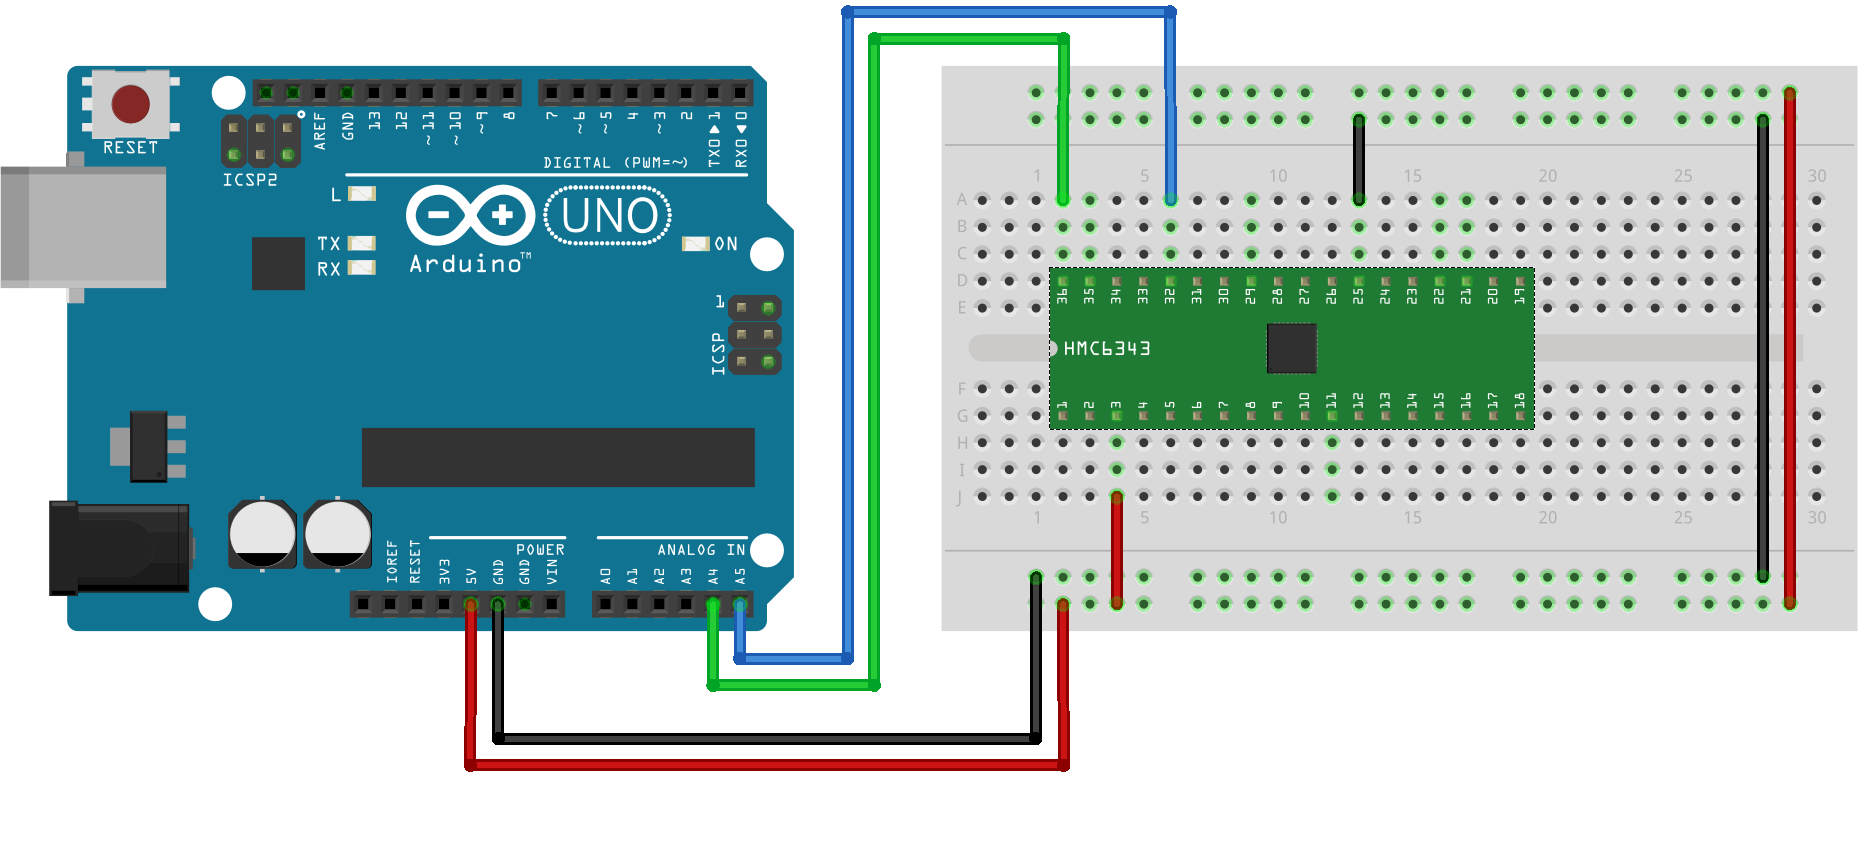
\includegraphics[width=\linewidth]{arduino_wiring_hmc.png}
  \caption{Example wiring for Arduino with HMC6343 for joystick operation.}
  \label{arduino_wiring_hmc.png}
\end{figure}

%=====================

\begin{table}
\begin{center}
\begin{minipage}{.45\linewidth}
\begin{center}
\begin{tabularx}{\textwidth}{c *{2}{>{\centering\arraybackslash}X}}
\toprule
\textbf{HMC6343 pin} & \textbf{Arduino Uno R3 pin} \\
\midrule
VCC & 5V\HMCvccFootnote{} \\

GND & GND \\

SDA & A4\itwocFootnote{} \\

SCL & A5 \\
\bottomrule
\end{tabularx}
\end{center}
\end{minipage}
\end{center}
\caption{Pin designation for figure \ref{arduino_wiring_hmc.png}.}
\label{HMC6343wiringtable}
\end{table}

%=====================

\begin{figure}[h]
\centering
  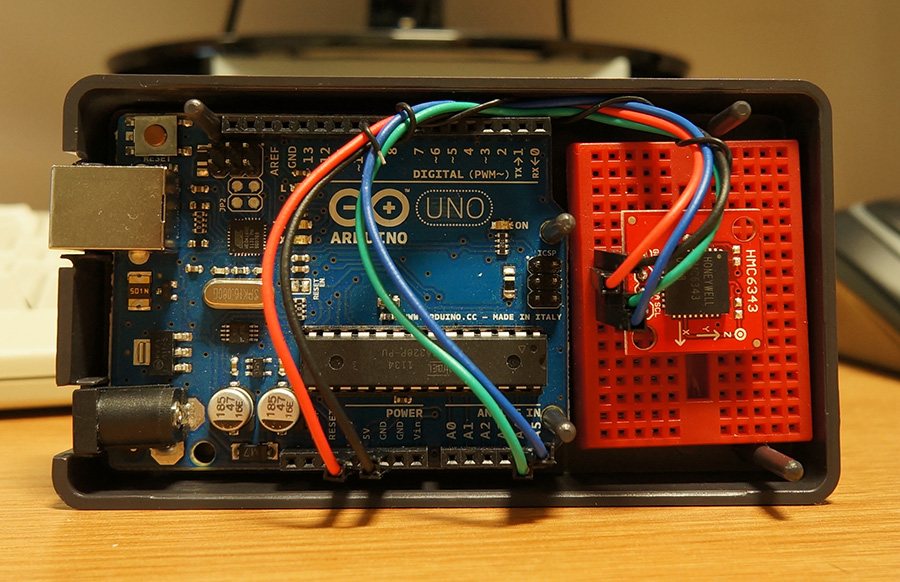
\includegraphics[width=.6\linewidth]{arduino_joystick_for_second_life_1.jpg}
  \caption{Assembled Arduino Uno R3 + HMC6343.}
  \label{arduino_joystick_for_second_life_1.jpg}
\end{figure}

A magnetometer used alone is only capable of providing a meaningful compass bearing when held level. In the case of applications where a compass bearing is required of a device that is not maintained level, such as in the case of VTW, the non-level orientation of the device must be taken into account to offset the readings of the magnetometer \& provide a correct compass bearing. The HMC6343's combination of magnetometer, accelerometer \& algorithms provides a single package that internally performs this process, using the readings from its accelerometer to compensate the readings from its magnetometer \& provide a meaningful compass bearing in non-level orientations.

Further requirements for obtaining accurate compass bearings from a MEMS magnetometer are to account for distortions to the magnetic field it senses \& to compensate the bearings it reports for the amount of magnetic declination for the location \& date wherein it is being used. Various materials that influence magnetic fields or produce their own magnetic field will distort the Earth's magnetic field \& thus impact the readings that a MEMS magnetometer collects. In the case of VTW, the sources of primary consideration are the electronics of the Arduino, tablet \& associated wiring. Due to the nature of these sources \& the fact that they are permanently situated \& attached to the same frame of reference as the magnetometer, moving as it moves, the distortions can be mitigated using a hard iron offset approach. Magnetic declination refers to the difference between `magnetic north' \& geographic `true north'. This value varies depending upon world location \& changes over time, so must be updated when the magnetometer is deployed to a different location or used at a subsequent date.

%***Reference for hard iron offset - here or later where we talk about the hex?

%=========================================================================================================

\subsection{Exploiting Second Life's Joystick Support}

\label{exploitJoystick}

\newcommand{\ArduinoJoystickVideoFootnote}{\footnote{\url{https://www.youtube.com/watch?v=-ddtmqoGNmg}}}

\newcommand{\atmegaFootnote}{\footnote{\url{http://www.atmel.com/devices/ATMEGA16U2.aspx}}}

\newcommand{\atmegaTFootnote}{\footnote{\url{http://www.atmel.com/devices/atmega328.aspx}}}

\newcommand{\arduinousbhidFootnote}{\footnote{\url{http://hunt.net.nz/users/darran/weblog/a3599/}}}

\newcommand{\lufaFootnote}{\footnote{\url{http://www.fourwalledcubicle.com/LUFA.php}}}

%=====================

As highlighted in section \ref{SecondLifeMobility} the Second Life client can be controlled only via mouse, keyboard \& joystick. Using the HMC6343's compass bearing \& yaw values therefore requires one of two approaches;

\begin{enumerate}
	\item Encapsulating the compass bearing \& yaw values into mouse, keyboard \&/or joystick commands;
	\item Modification to the Second Life client to allow the compass bearing \& yaw values to be used directly at a lower level of abstraction.
\end{enumerate}

Method 1 has the advantage of having no reliance upon any particular Second Life client, as all available clients are forks of the official client from Linden Lab \& maintain the same keyboard, mouse \& joystick interfaces. However if the level of control attainable by re-purposing these interfaces for control from magnetometer \& accelerometer data is not enough, method 2 will be the only option.

Conceptually, all Arduino boards are programmed over an RS-232 serial connection. When the platform was first launched, the Arduino boards themselves had a physical DE-9 serial connector with which to connect to a host computer's serial connector. But as serial connectors all but disappeared from modern computers, the Arduino's serial connector was replaced in later revisions with a USB connector, as USB is now all but ubiquitous on today's computers. The move from a physical RS-232 connector to a USB connector requires additional hardware upon the Arduino board to convert between RS-232 \& USB, as the ATMega328\atmegaTFootnote{} microcontroller at the heart of the Arduino Uno R3 does not have a USB interface itself. For this reason the current revision, the Arduino Uno R3, sports an ATMega16U2\atmegaFootnote{} microcontroller that serves to convert communications between the two standards, RS-232 \& USB.

With its stock firmware, the Arduino's ATMega16U2 presents itself to the host computer as a USB-to-serial bridge. However the ATMega16U2 can have this stock firmware replaced in order to change its behaviour. One of these new behaviours is to act as a USB Human Interface Device (HID) class controller, identifying itself to the host computer as one of a myriad input devices - including joysticks. Using a USB HID class joystick firmware for the ATMega16U2\arduinousbhidFootnote{}, based upon the Lightweight USB Framework for AVRs (LUFA)\lufaFootnote{}, the Arduino can imitate a standard USB joystick, sending joystick commands to the host computer using the protocol in the USB specification.

%***How to flash the firmware

In this manner, the Arduino can marshal the values obtained from the HMC6343 into standard USB HID joystick commands, allowing the Second Life client's stock joystick interface (see figure \ref{arduino_joystick_for_second_life_3.jpg}) to be used to control the camera orientation (\& avatar movement) according to the physical orientation of the HMC6343, as can be seen in\ArduinoJoystickVideoFootnote{}.

\begin{figure}[h]
\centering
  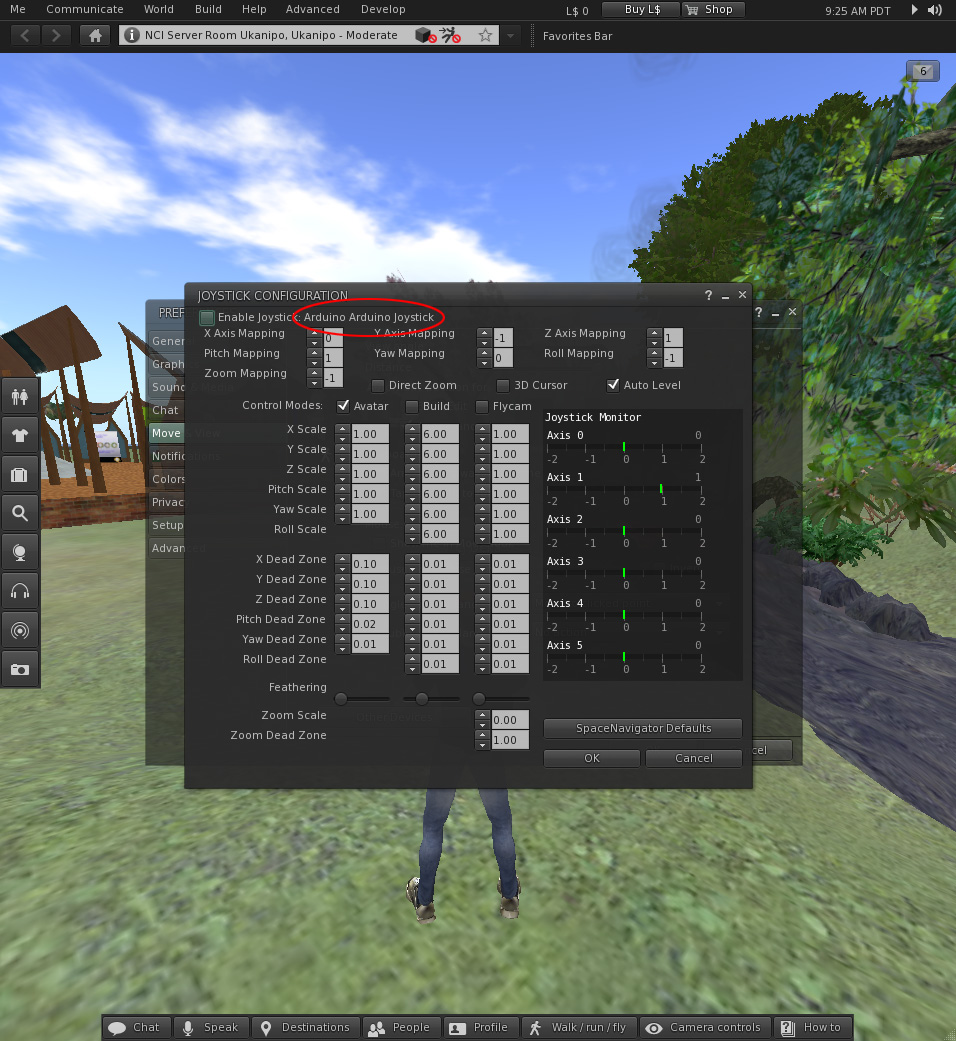
\includegraphics[width=.7\linewidth]{arduino_joystick_for_second_life_3.jpg}
  \caption{Configuration in Second Life client for Arduino + HMC6343 `joystick'.}
  \label{arduino_joystick_for_second_life_3.jpg}
\end{figure}

Unfortunately, the precision attainable through this approach is not sufficient for the style of control \& interaction required for VTW. Specifically, the Second Life client's joystick interface applies smoothing/damping to the joystick inputs, preventing reliable rotations or movements of specific values - sending a joystick command to rotate the camera by $x$\textdegree\ followed by a second command to rotate the camera by $-x$\textdegree\ does not reliably return the camera to its original orientation before the application of the first rotation. As the interaction required is to map the \textit{absolute} orientation of the tablet to the Second Life camera, this discrepancy (which cannot be disabled from the Second Life client's joystick configuration) renders the approach unworkable.

%=========================================================================================================

\section{Position Control}
\label{second_life_position_control}

In order to control the position of the Second Life avatar, sensor data are required for the position of the user in the real world. As the cultural heritage sites that VTW was intended for use upon are outdoor sites, namely those where there are traces of ruins \& clear views of the sky, GPS is the logical choice for tracking user position. GPS has been widely used as a localization technique within virtual heritage, particularly for AR applications.

%***diagram showing this

In order for readings from a GPS receiver to be used to control the position of the Second Life avatar within a reconstruction, a translation must be performed between the coordinate system of GPS (latitude \& longitude) \& the coordinate system of Second Life (simple X,Y coordinates within 256 metre square `regions'). This is achieved by use of a single `anchor point', for which both the real world latitude \& longitude \& the corresponding virtual world X,Y coordinates are known. Calculating Second Life displacement from these X,Y coordinates is achieved by applying the scale of the reconstruction to the displacement between the anchor point's latitude \& longitude \& the user's current position reported as latitude \& longitude by a GPS receiver. This real world displacement is calculated using the haversine formula~\cite{VanBrummelen2012}, which is used to calculate the `great circle' (orthodromic) distance between two points on the surface of a sphere (such as the Earth, when simplified from its oblate spheroid shape). The central angle \text{$\left(\frac{d}{r}\right)$} between the two points is given by;

\begin{equation}
\label{haversine1}
\text{haversin}\left(\frac{d}{r}\right) = \text{haversin}(\phi_{2}-\phi_{1})+\cos(\phi_{1})\cos(\phi_{2})\text{haversin}(\lambda_{2}-\lambda_{1})
\end{equation}

where;

\begin{itemize}
	\item \text{haversin} is the haversine function
		\begin{equation}
		\label{harsine2}
			\text{haversin}(\theta) = \sin^{2}\left( \frac{\theta}{2}\right) = \frac{1-\cos(\theta)}{2}
		\end{equation}
	\item $d$ is the distance between the two points along a great circle of the sphere,
	\item $r$ is the radius of the sphere,
	\item \text{$\phi_{1},\phi_{2}$} are the latitudes of point 1 \& point 2,
	\item \text{$\lambda_{1},\lambda_{2}$} are the longitudes of point 1 \& point 2.
\end{itemize}

The equation can be solved for the distance $d$ by applying the inverse haversine function or through application of arcsine;

\begin{equation}
	\label{haversine3}
	d = r\;\text{haversin}^{-1}\left( h \right) = 2r \arcsin \left( \sqrt{h} \right)
\end{equation}

where $h$ is $\text{haversin}\left( \frac{d}{r} \right)$;

\begin{align}
d & = 2r \arcsin\left( \sqrt{\text{haversin} \left( \phi_{2} - \phi_{1} \right) + \cos \left( \phi_{1} \right) \cos  \left( \phi_{2} \right) \text{haversin} \left( \lambda_{2} - \lambda_{1} \right) } \right) \nonumber \\ 
& = 2r \arcsin\left( \sqrt{\sin^{2} \left( \frac{\phi_{2} - \phi_{1}}{2}\right) + \cos\left( \phi_{1} \right) \cos\left( \phi_{2} \right) \sin^{2} \left( \frac{\lambda_{2} - \lambda_{1}}{2} \right) } \right)
\end{align}

The prerequisites for this approach are that the Second Life model is aligned correctly to the Second Life compass as the real location is aligned to real bearings (also required for orientation control from the previous section), a single anchor point for which both the real world latitude \& longitude \& the corresponding virtual world X \& Y coordinates are known \& that the reconstruction adheres to a known, consistent scale.

Figure \ref{haversine_example.png} illustrates this arrangement. In the real world, on the left, we know the latitude \& longitude of the anchor point, as well as the latitude \& longitude of the user's current position as reported by the GPS receiver. In the virtual world, on the right, we know the X,Y coordinates that are equivalent to the latitude \& longitude of the anchor point \& we must calculate the X,Y coordinates that are equivalent to the user's current position as reported by the GPS receiver.

\begin{figure}[h]
\centering
  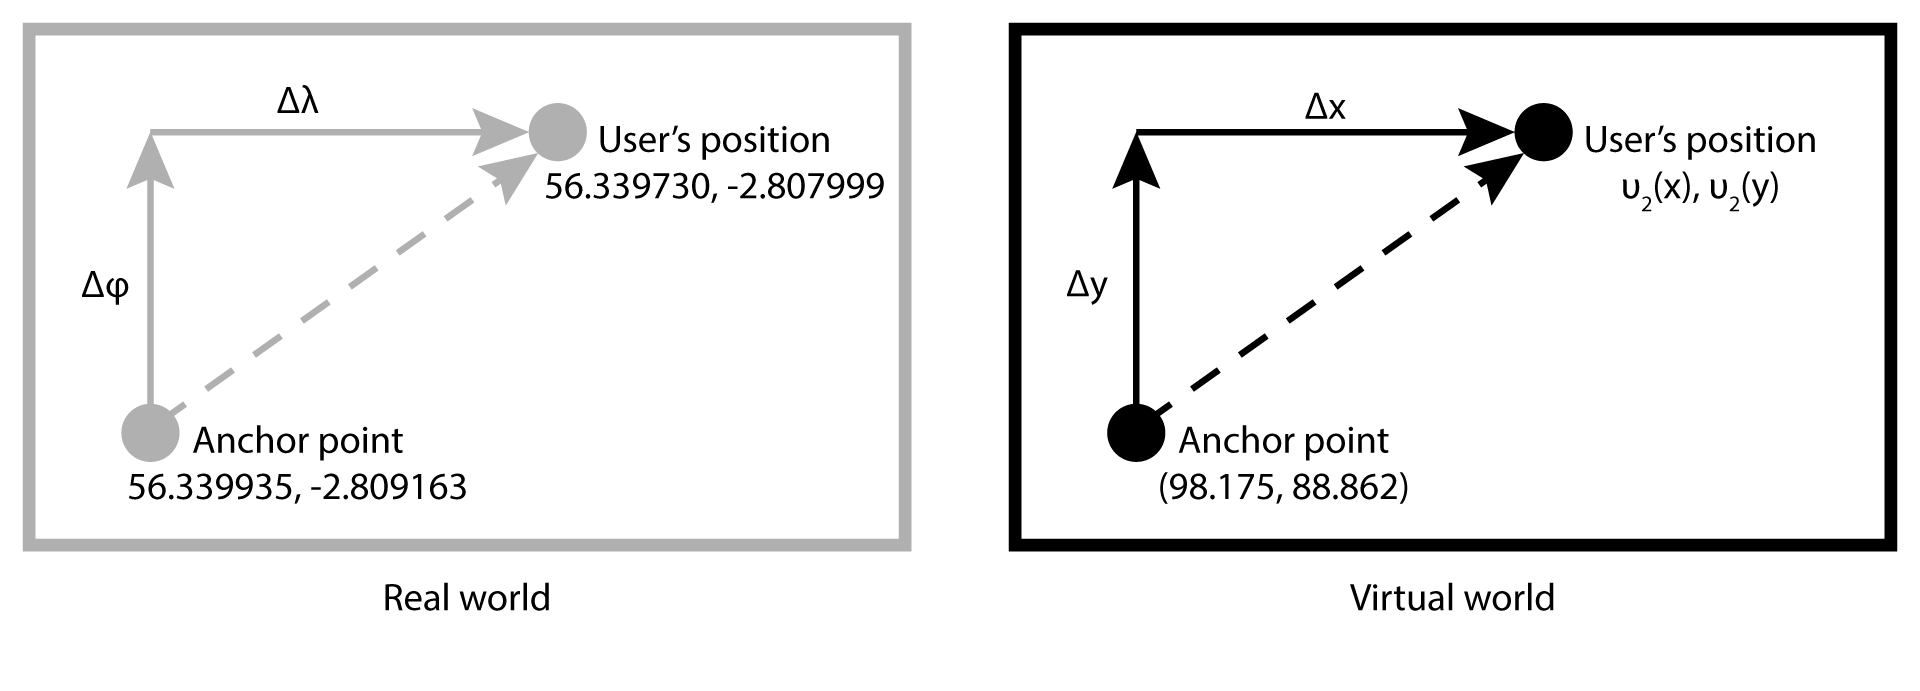
\includegraphics[width=\linewidth]{haversine_example.png}
  \caption{Using haversine to mimic real world movement in a virtual world.}
  \label{haversine_example.png}
\end{figure}

The difference in longitude between the anchor point \& the user's position, $\Delta\lambda$, is given by;

\begin{equation}
2r \arcsin\left( \sqrt{\sin^{2} \left( \frac{\lambda_{2} - \lambda_{1}}{2} \right) } \right)
\end{equation}

While the difference in latitude between the anchor point \& the user's position, $\Delta\phi$, is given by;

\begin{equation}
2r \arcsin\left( \sqrt{\sin^{2} \left( \frac{\phi_{2} - \phi_{1}}{2}\right)} \right)
\end{equation}

Applying the scale of the reconstruction to these values gives $\Delta$x \& $\Delta$y, which can then be added or subtracted from the X,Y coordinates of the anchor point to give the coordinates of the user's position, $\upsilon_{2}(x),\upsilon_{2}(y)$.

%Using the haversine formula the great-circle (or orthodromic) distance between the latitude of the anchor point and the latitude of the new GPS reading is calculated, then applying the scale of the model results in the equivalent distance in OpenSim metrics between the Y coordinate of the anchor point and the Y coordinate of the position corresponding to the new GPS reading. Repeating the same calculations with the longitude of the new GPS reading provides the distance between the X coordinate of the anchor point and the X coordinate of the position corresponding to the new GPS reading. Adding or subtracting these distances as appropriate to the OpenSim coordinates of the anchor point provides the OpenSim coordinates that correspond to the new GPS reading, to which the avatar is then instructed to move.

%The anchor point is specified using global coordinates, not local coordinates. This allows navigation to operate across region boundaries and within mega regions (it is not limited to a single 256x256 meter OpenSim region) and there are no restrictions for the placement of the OpenSim component of the anchor point (it can be anywhere in any region, movement of the avatar can be in any direction from it (positive and negative), it does not have to be at the center of the model or even in a region that the model occupies).

%Calculating a global coordinate is simply a case of multiplying the position of the region by 256 and then adding the local coordinate. For example, for an anchor at local coordinate $(127,203,23)$ within a region that is at $(1020,1042)$ the global X coordinate is calculated as $(1020 * 256) + 127 = 261247$ and the global Y coordinate as $(1043 * 256) + 203 = 267211$. Elevation (Z) is ignored due to a combination of the relatively low accuracy of these data attainable via GPS (when compared to the longitudinal/latitudinal accuracy) and as the case study explored involved users navigating outdoor ruins remaining at ground level.

%=========================================================================================================

\subsection{GPS Receivers}

\newcommand{\azurewaveFootnote}{\footnote{\url{http://www.azurewave.com/product_GPS-M19_1.asp}}}

\newcommand{\habFootnote}{\footnote{\url{http://ukhas.org.uk/}}}

\newcommand{\ubloxFootnote}{\footnote{\url{https://u-blox.com/en/gps-modules/pvt-modules/previous-generations/max-6.html}}}

\newcommand{\sarantelFootnote}{\footnote{\url{http://www.sarantel.com/sl1200_(33).html}}}

\newcommand{\MAXvccFootnote}{\footnote{The MAX-6 requires 2.5 to 3.6V input on VCC, this table showing connection to 5V assumes a MAX-6 breakout with appropriate step down.}}

\newcommand{\MAXserialFootnote}{\footnote{The data pins of the MAX-6 need to be pulled up to between 0.7 to 1.0 of the supply to VCC, so a breakout with appropriate level shifters is required for connection directly to an Ardunio Uno R3's 5V digital pins.}}

\newcommand{\softwareserialFootnote}{\footnote{\url{http://arduino.cc/en/Reference/SoftwareSerial}}}

\newcommand{\maxProtocolFootnote}{\footnote{\url{https://u-blox.com/images/downloads/Product_Docs/u-blox6_ReceiverDescriptionProtocolSpec_(GPS.G6-SW-10018).pdf}}}

\newcommand{\tinygpsFootnote}{\footnote{\url{http://arduiniana.org/libraries/tinygps/}}}

%=====================

The WindPad features an internal AzureWave GPS-M16 GPS receiver\azurewaveFootnote{}, however poor API provision and meagre documentation required the adoption of an alternative receiver. As an Arduino was already being used to provide orientation data from accelerometer \& magnetometer, integrating the GPS receiver into this package such that all orientation \& position data came from a single source seemed prudent. After receiving input \& advice from the UK High Altitude Society\habFootnote{}, \textit{``a loose collection of people who are interested in launching unmanned high altitude balloons into near space''} who make extensive use of GPS receivers for tracking their launches, the u-blox MAX-6\ubloxFootnote{} GPS receiver outfitted with a Sarantel SL-1202\sarantelFootnote{} passive antenna was chosen to provide position data for the VTW platform. The MAX-6 is of higher operational specification than the GPS-M16 and supports Satellite Based Augmentation Systems (SBAS) which improve the accuracy of location data by applying additional correction data received from networks of satellites and ground-based transmitters separate to those of the GPS system. These networks include the European Geostationary Navigation Overlay Service (EGNOS) that covers the UK where the experiments took place.

Figure \ref{arduino_wiring_hmc_ublox.png} provides a wiring diagram for connectivity of a u-blox MAX-6 to an Arduino Uno R3, along with the HMC6343 from section \ref{OrientationControl}, with the pinout values provided by tables \ref{HMC6343_MAX6_wiringtable_HMC6343} \& \ref{HMC6343_MAX6_wiringtable_MAX6}. The LED \& 220$\Omega$ resistor on digital pin 12 is used for diagnostic output. The wiring shown here for a MAX-6 breakout without I2C connectivity, instead using Arduino's SoftwareSerial\softwareserialFootnote{} library.

\begin{figure}[h]
\centering
  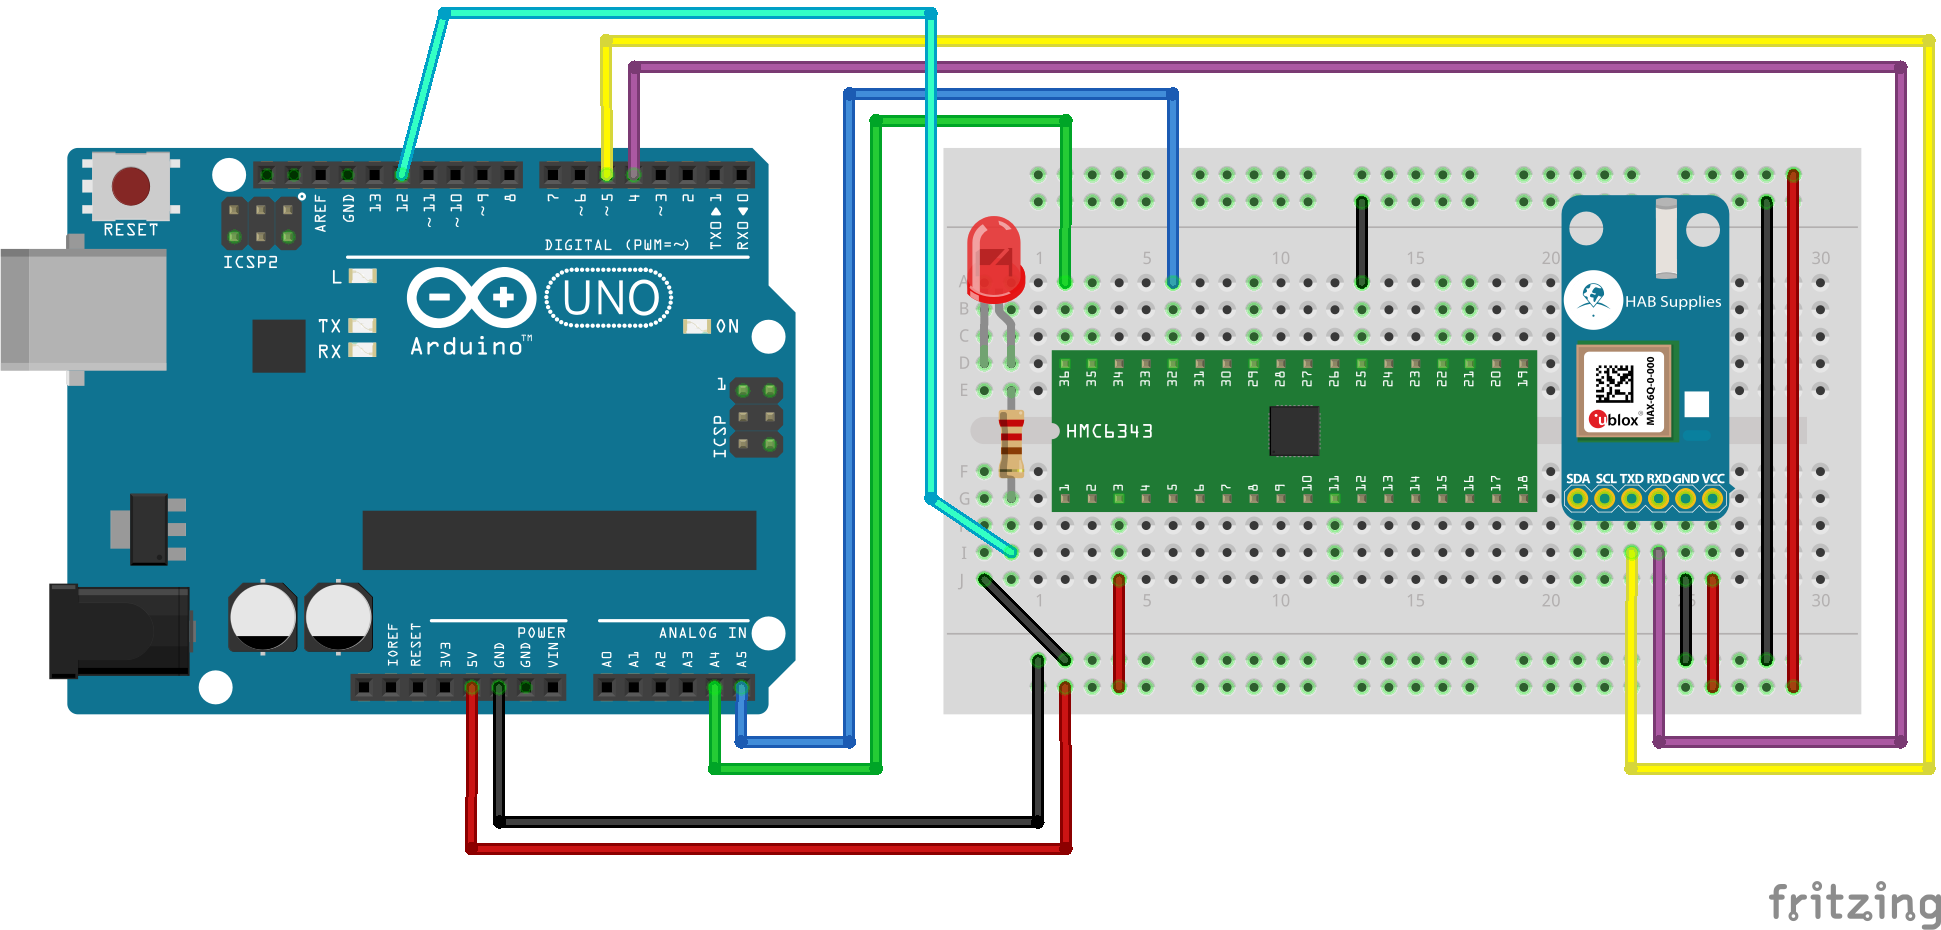
\includegraphics[width=\linewidth]{arduino_wiring_hmc_ublox.png}
  \caption{Example wiring for Arduino with HMC6343 + u-blox MAX-6.}
  \label{arduino_wiring_hmc_ublox.png}
\end{figure}

\begin{table}
\begin{center}
\begin{minipage}[t]{.45\linewidth}
\begin{center}
\begin{tabularx}{\textwidth}{c *{2}{>{\centering\arraybackslash}X}}
\toprule
\textbf{HMC6343 pin} & \textbf{Arduino Uno R3 pin} \\
\midrule
VCC & 5V\HMCvccFootnote{} \\

GND & GND \\

SDA & A4\itwocFootnote{} \\

SCL & A5 \\
\bottomrule
\end{tabularx}
\caption{Pin designation for figure \ref{arduino_wiring_hmc_ublox.png} (HMC6343).}
\label{HMC6343_MAX6_wiringtable_HMC6343}
\end{center}
\end{minipage}
%
\begin{minipage}[t]{.02\linewidth}
\hfill%
\end{minipage}
%
\begin{minipage}[t]{.45\linewidth}
\begin{center}
\begin{tabularx}{\textwidth}{c *{2}{>{\centering\arraybackslash}X}}
\toprule
\textbf{MAX-6 pin} & \textbf{Arduino Uno R3 pin} \\
\midrule
VCC & 5V\MAXvccFootnote{} \\

GND & GND \\

RXD & D4 \MAXserialFootnote{}\\

TXD & D5 \\
\bottomrule
\end{tabularx}
\caption{Pin designation for figure \ref{arduino_wiring_hmc_ublox.png} (MAX-6).}
\label{HMC6343_MAX6_wiringtable_MAX6}
\end{center}
\end{minipage}
\end{center}
\end{table}

Figure \ref{arduino_hmc6343_u-blox_MAX-6.jpg} shows an the assembled unit, comprising an Arduino Uno R3, prototyping shield, HMC6343 \& MAX-6, while figure \ref{pangolin_tablet_back.jpg} shows the packaged unit attached to the back of the WindPad.

\TwoFig{arduino_hmc6343_u-blox_MAX-6.jpg} {Assembled Arduino/sensors.} {arduino_hmc6343_u-blox_MAX-6.jpg}
       {pangolin_tablet_back.jpg} {Arduino/sensors attached to tabet.} {pangolin_tablet_back.jpg}
       
%=========================================================================================================

The MAX-6 is configured as follows;

\begin{enumerate}
	\item Dynamic Platform Model set to Pedestrian.
	\item SBAS via EGNOS is enabled,
	\item GPGLL/GPGSA/GPGSV/GPVTG messages are disabled,
	\item GPRMC/GPGGA messages are enabled.
\end{enumerate}

The Dynamic Platform Models adjust how the navigation engine processes the readings that the receiver produces \& by choosing the correct model for the receiver's application accuracy of position output is increased. As VTW is an application in which the user walks about an outdoor cultural heritage site, the pedestrian model is most suitable. Satellite Based Augmentation System (SBAS) is enabled for the European Geostationary Navigation Overlay Service (EGNOS), which is available at the cultural heritage sites in Scotland that VTW will be used at, to improve the accuracy of the position output.

The output of the receiver is in the form of messages in the NMEA 0183 protocol from the National Marine Electronics Association. By default, the MAX-6 sends many more message types than are required for VTW \& as the Arduino's processing power is limited the superfluous messages are disabled. The GPRMC message format contains the recommended minimum amount of information for transit applications, including time, latitude \& longitude.

These configurations are effected by sending the MAX-6 commands encoded in the UBX protocol as arrays of hex values. For example, setting the Dynamic Platform Model to Pedestrian is performed with the code in figure \ref{arduinoMAX6hex}, where \path{sendUBX} is a function that writes out using SoftwareSerial;

\begin{figure}[h]
\begin{lstlisting}[language=C, numbers=left, numberstyle=\small, stepnumber=1, frame=single, breaklines=true, backgroundcolor=\color{codebackground}, showstringspaces=false]
uint8_t CFG_NAV5[] = {0xB5, 0x62, 0x06, 0x24, 0x24, 0x00, 0xFF, 0xFF,
                      0x03, 0x03, 0x00, 0x00, 0x00, 0x00, 0x10, 0x27,
                      0x00, 0x00, 0x05, 0x00, 0xFA, 0x00, 0xFA, 0x00,
                      0x64, 0x00, 0x2C, 0x01, 0x32, 0x3C, 0x00, 0x00,
                      0x00, 0x00, 0x00, 0x00, 0x00, 0x00, 0x00, 0x00,
                      0x00, 0x00, 0x00, 0x00};
calculateUBXChecksum(CFG_NAV5, (sizeof(CFG_NAV5)/sizeof(uint8_t)));

while (!success)
{
  sendUBX(CFG_NAV5, (sizeof(CFG_NAV5)/sizeof(uint8_t)));
  success = getUBX_ACK(CFG_NAV5);
}
success = 0;
\end{lstlisting}
\caption{Setting MAX-6 Dynamic Platform Model to Pedestrian in an Arduino sketch.}
\label{arduinoMAX6hex}
\end{figure}

These hex arrays can be generated by hand from the UBX protocol specification\maxProtocolFootnote{}, or the MAX-6 can be configured by connecting it directly to a host computer (such as by using an Arduino as an UART by connecting the MAX-6 to digital pins 0 \& 1), configuring the MAX-6 using the u-blox u-center software \& then copying the resultant config as hex messages from the relevant console window.

NMEA messages from the MAX-6 are processed on the Arduino using the TinyGPS library\tinygpsFootnote{}, extracting the latitude \& longitude values before combining them with magnetic compass bearing (yaw) \& pitch values from the HMC6343 \& sending these to the host computer via the Arduino's USB connective.

%=========================================================================================================

\subsection{OpenSim Region Module}

\label{regionModule}

\newcommand{\RegionModuleFootnote}{\footnote{\url{http://opensimulator.org/wiki/IRegionModule}}}

\newcommand{\RegionModuleCodeFootnote}{\footnote{\url{https://bitbucket.org/cj_davies/sharedregionmodulegpsavatar}}}

%=====================

One of the extensions that the OpenSim server provides over the Second Life server that it emulates, is extensibility via Region Modules.

\begin{quotation}
	\textit{``Region modules are .net/mono DLLs. During initialization of the simulator, the OpenSimulator bin directory (bin/) and the scriptengines (bin/ScriptEngines) directory are scanned for DLLs, in an attempt to load region modules stored there. Region modules execute within the heart of the simulator and have access to all its facilities. Typically, region modules register for a number of events, e.g. chat messages, user logins, texture transfers, and take what ever steps are appropriate for the purposes of the module.''}\RegionModuleFootnote{}
\end{quotation}

Region modules allow for more complex \& powerful extensions, written in C\#, to be developed external to the OpenSim platform than would otherwise be possible via Second Life's internal Linden Scripting Language (LSL). Similar to how the Second Life client's joystick interface represented an opportunity to implement the orientation control of VTW without relying upon a bespoke, modified client, an OpenSim Region Module represents the possibility to implement the position control required by VTW without relying upon a similarly bespoke client.

An excerpt from the implementation of the position control required by VTW is included as \ref{RegionModuleCode1} (full Region Module code available online\RegionModuleCodeFootnote{}). This shows the use of haversine, implemented using the \texttt{atan2()} function, calculating the displacement in real world latitude between the anchor point \& the new GPS reading (lines 5-8), applying the scale of the reconstruction to this displacement (lines 10-14) \& then applying this scaled displacement to the virtual world Y coordinate of the anchor (lines 16-24). This process is then repeated for the longitude/X coordinate \& the avatar can then be moved to the position within the OpenSim reconstruction that is equivalent to the user's new real world position.

\begin{figure}[h]
\begin{lstlisting}[language=Java, numbers=left, numberstyle=\small, stepnumber=1, frame=single, breaklines=true, backgroundcolor=\color{codebackground}, showstringspaces=false]
private Vector3 LatitudeLongitudeToRegionCoordinate(double newLat, double newLong, double anchorLat, double anchorLong, Vector3 anchorVector, double scale) {

    double d, a, c, X, Y;

    //calculate the difference in y (latitude) between the anchor & the new reading
    d = Math.Abs(ToRadians(newLat - anchorLat));
    a = Math.Sin(d / 2) * Math.Sin(d / 2);
    c = 2 * Math.Atan2(Math.Sqrt(a), Math.Sqrt(1 - a));

    //mean radius of the Earth is 6371km (6371000m)
    d = 6371000 * c;

    //apply scale
    d *= scale;

    //sum appropriately from the anchor
    if (newLat > anchorLat) {
        mlog.DebugFormat("[GPSAvatarModule]: LatitudeLongitudeToRegionCoordinate() - (Y) newLat > anchorLat.");
        Y = (anchorVector.Y + d);
    }
    else {
        mlog.DebugFormat("[GPSAvatarModule]: LatitudeLongitudeToRegionCoordinate() - (Y) newLat < anchorLat.");
        Y = (anchorVector.Y - d);
    }
\end{lstlisting}
\caption{Excerpt of OpenSim Region Module for avatar movement via GPS.}
\label{RegionModuleCode1}
\end{figure}

%=========================================================================================================

%\clearpage

%=========================================================================================================

\section{Modifying Second Life for Orientation \& Position Control}

Due to the Second Life client's existing control interfaces not allowing enough control over camera orientation for VTW's requirements (section \ref{exploitJoystick}), it was necessary to modify the client's codebase to produce a bespoke client allowing complete control over orientation by magnetometer \& accelerometer input. Although sufficient position control could be achieved via an OpenSim region module (section \ref{regionModule}) it was prudent to also encapsulate position control through the modified client; not only does this allow for finer grain control, it also removes the dependency upon the virtual reconstruction being hosted upon an OpenSim server (Second Life's own servers do not support extension via Region Modules). Thus, the Second Life client was modified with the addition of the ability to;

\begin{itemize}
	\item connect to a serial device for I/O,
	\item control movement of the avatar according to input from this serial device,
	\item control the camera according to input from this serial device.
\end{itemize}

%=========================================================================================================

\subsection{Overview of Second Life Client Modifications}

\newcommand{\asioFootnote}{\footnote{\url{http://www.boost.org/doc/libs/1_57_0/doc/html/boost_asio.html}}}

\newcommand{\boostFootnote}{\footnote{\url{http://www.boost.org/}}}

\newcommand{\fedetftFootnote}{\footnote{\url{http://www.webalice.it/fede.tft/serial_port/serial_port.html}}}

\newcommand{\regionmodulelimitationFootnote}{\footnote{This is not due to any limitation on the part of OpenSim, but simply due to the Second Life client modifications being pursued further than the OpenSim module.}}

\newcommand{\megaregionFootnote}{\footnote{\url{http://opensimulator.org/wiki/Setting_Up_Mega-Regions}}}

%=====================

%Replaced the Linden Boost binary with that built by LightDrake

The Second Life client is written predominantly in C++ so the Asio library\asioFootnote{} from the popular Boost project\boostFootnote{} is used to imbue it with serial connectivity, allowing it to receive messages from the Arduino in an asynchronous non-blocking fashion. The fundamental buffered asynchronous serial handling is implemented using Terraneo Federico's \path{AsyncSerial} class\fedetftFootnote{} which is included in the client codebase as \path{/indra/newview/AsyncSerial}. The majority of the functionality added to the client is then contained within \path{/indra/newview/LLViewerSerialMovement}. The core executable of the viewer, \path{/indra/newview/LLAppViewer} obtains an instance of \path{LLViewerSerialMovement} \& then calls \path{LLViewerSerialMovement::update()} upon each iteration of the client's main update loop, \path{LLAppViewer::mainLoop()}. These modifications are visualised by figure \ref{second_life_structure.png}.

\begin{figure}[h]
\centering
  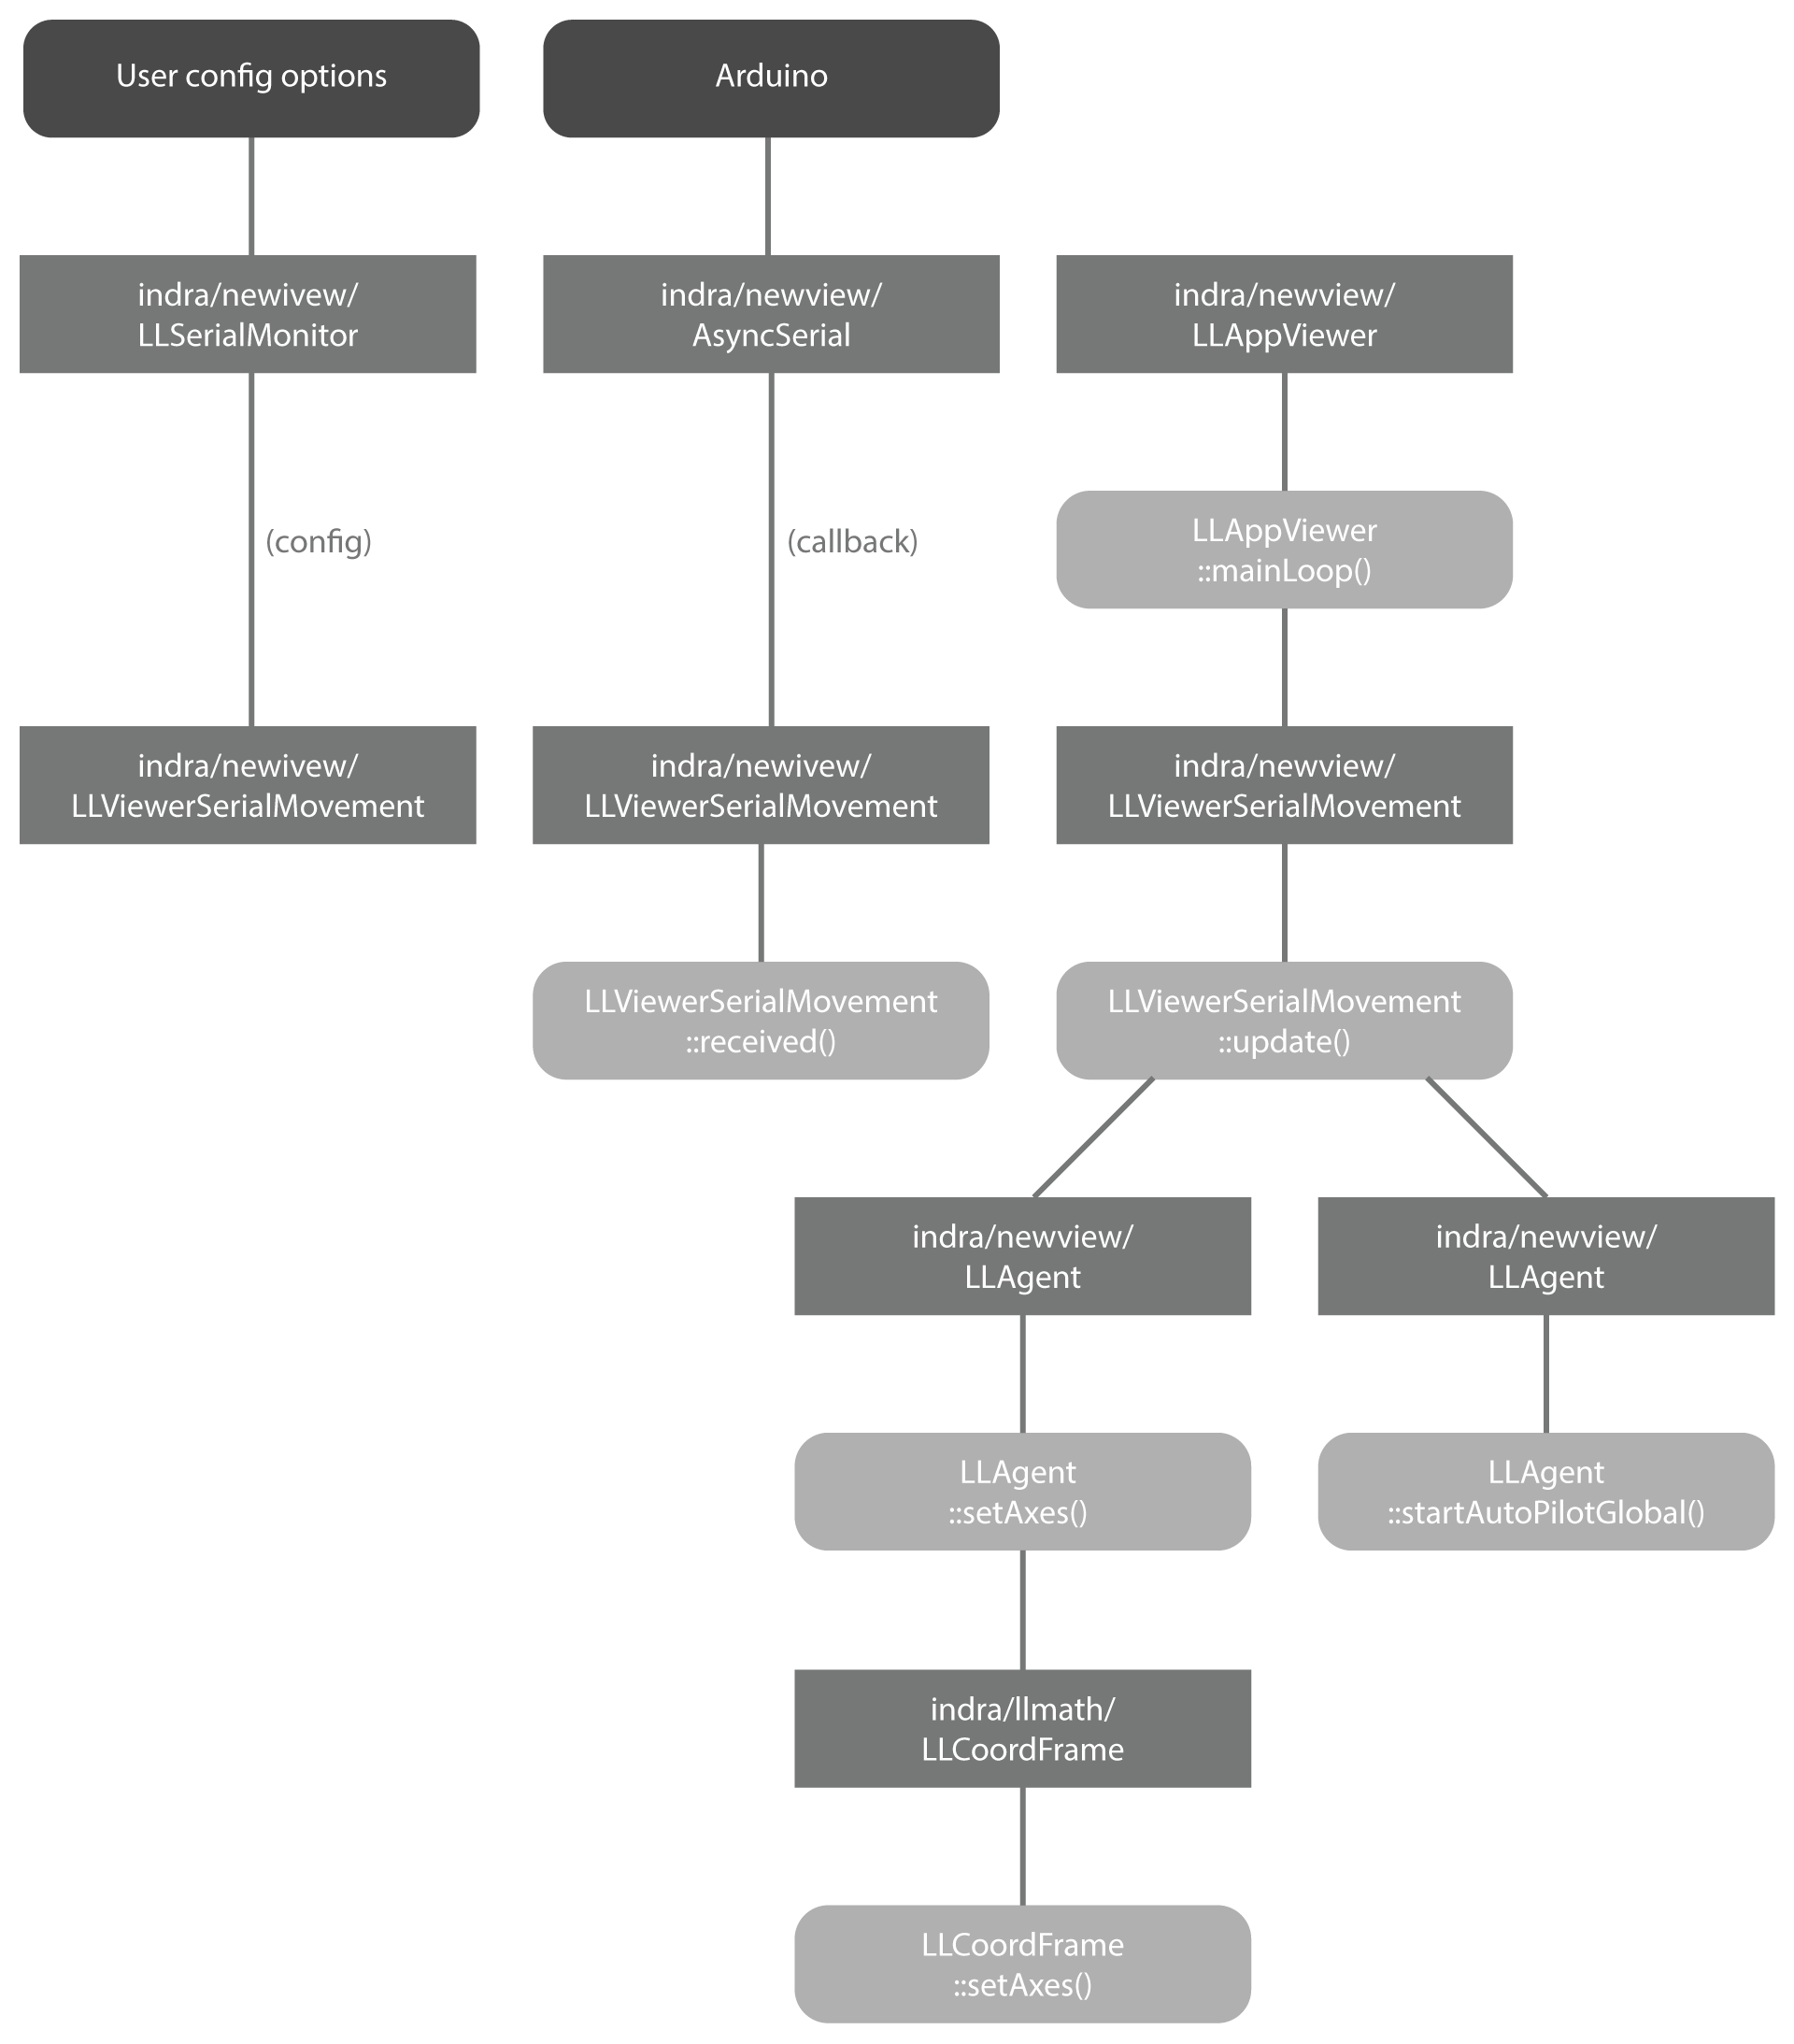
\includegraphics[width=.8\linewidth]{second_life_structure.png}
  \caption{Overview of modifications to Second Life client.}
  \label{second_life_structure.png}
\end{figure}

%=========================================================================================================

\subsection{\texttt{LLViewerSerialMovement} reference}
Brief documentation of the functions in \path{/indra/newview/LLViewerSerialMovement} follows.
\begin{center}
\begin{longtable}{ p{4.2cm}  p{10cm} }

\toprule

\textbf{Function} & \textbf{Description} \\

\midrule

%=========================================================================================================
		
\texttt{::connect} & Safely connects to a serial device (if not already connected). \\
		
\midrule

%=========================================================================================================

\texttt{::disconnect} & Safely disconnects from a serial device (if already connected). \\
		
\midrule

%=========================================================================================================

\texttt{::received} & A callback method registered to the \path{CallbackAsyncSerial} class in \path{/indra/newview/AsyncSerial}. This function parses the data (\path{const} \path{char} \path{*data}) from the serial device, extracting complete messages to the variable \path{mostRecentMessage}. Because of the nature of the serial I/O, \path{*data} is not guaranteed to contain a discrete message from the Arduino containing both orientation \& position data, thus this function must parse the array \& assemble discrete messages from possibly multiple subsequent callbacks. \\
		
\midrule

%=========================================================================================================

\texttt{::update} & Called upon each iteration of \path{LLAppViwer::mainLoop()} \& further calls \path{::updateFromMostRecentMessage()}, \path{::updateOrientation()} \& \path{::updatePosition()}. \\
		
\midrule

%=========================================================================================================

\texttt{::updateFromMostRecent- Message} & Processes a complete message from the Arduino which has been assembled by \path{::received()} \& extracts the constituent orientation \& position values. \\
		
\midrule

%=========================================================================================================

\texttt{::updateOrientation} & Applies the orientation values extracted from an Arduino message to the avatar's camera. This is achieved by a call to \path{LLAgent::setAxes()} which calls \path{LLCoordFrame::setAxes()} in \path{/indra/llmath/LLCoordFrame}. The orientation values are passed as a quaternion, converting the bearing, pitch \& roll values extracted from the Arduino message as degrees using \path{::quaternionFromDegrees()}.\\
		
\midrule

%=========================================================================================================

\texttt{::updatePosition} & Applies the position data extracted from an Arduino message to the avatar, using \path{LLAgent::startAutoPilotGlobal()} to perform smooth movement between the avatar's current position (obtained with \path{LLAgent::getPositionGlobal()}) \& the new position from the Arduino (converted from latitude \& longitude to Second Life region coordinates in \path{::latitudeLongitudeToRegionCoordinates()}). \\
		
\midrule

%=========================================================================================================

\texttt{::quaternionFromDegrees} & A helper method to convert bearing, pitch \& roll expressed in degrees, into a single quaternion. Quaternions are frequently used to represent rotations in 3D applications, as they do not suffer from gimbal lock - Second Life is no exception to this \& internally uses quaternions for all rotation data, providing \path{/indra/llmath/LLQuaternion} for this purpose. \\
		
\midrule

%=========================================================================================================

\texttt{::latitudeLongitudeTo- RegionCoordinate} & Converts a real world position, expressed as a longitude \& latitude pair, to the equivalent Second Life coordinates, applying the haversine formula using knowledge of the real world \& corresponding Second Life position of the anchor point \& the scale of the Second Life reconstruction compared to the real world. \\
		
\midrule

%=========================================================================================================

\texttt{::degreesToRadians} & A helper method to convert values expressed in degrees to the equivalent value expressed in radians (implementations of the haversine formula usually make use of radians). \\
		
\bottomrule

%=========================================================================================================

\end{longtable}
\end{center}

%=========================================================================================================

Controlling the avatar's position according to latitude \& longitude readings from the GPS receiver is once again implemented using the haversine formula. This implementation, included as figure \ref{secondlifehaversine} can be compared to the OpenSim region module version included previously as figure \ref{RegionModuleCode1}. One important difference between the Second Life client implementation \& the OpenSim region module implementation is that the former uses global coordinates, rather than local coordinates\regionmodulelimitationFootnote{}. This means that the Second Life client implementation allows positional control of an avatar across region boundaries, crucial for use with a cultural heritage reconstruction that spans multiple regions in an OpenSim `megaregion'\megaregionFootnote{} such as that used for testing of VTW.

These modifications to the Second Life client are configured/controlled via a window added to the client \& accessed via a menu entry (see figure \ref{pangolin_second_life_dialogue.png}). The implementation of this resides in \path{/indra/newview/LLViewerSerialMonitor}. This allows for specification of the path to the serial device, along with its baudrate, as well as the specification of the anchor point - the latitude \& longitude of the point in the real world \& the equivalent X/Y coordinates in the Second Life reconstruction. The window then provides diagnostic output showing the messages coming in from the serial device, along with controls to individually enable/disable orientation \& position control \& alter the high-pass \& smoothing applied to both controls.

\begin{figure}[h]
\centering
  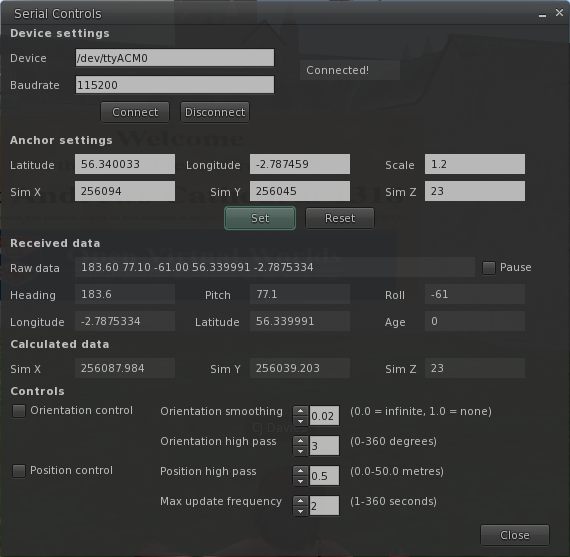
\includegraphics[width=0.6\linewidth]{pangolin_second_life_dialogue.png}
  \caption{Config pane in modified Second Life client for HMC6343 + MAX-6.}
  \label{pangolin_second_life_dialogue.png}
\end{figure}

\begin{figure}[h]
\begin{lstlisting}[language=C++, numbers=left, numberstyle=\small, stepnumber=1, frame=single, breaklines=true, backgroundcolor=\color{codebackground}, showstringspaces=false]
boost::tuple<float, float, float> LLViewerSerialMovement::latitudeLongitudeToRegionCoordinate(double newLat, double newLong, float anchorLat, float anchorLong, float scale, boost::tuple<float, float, float> anchorCoordinates) {

    double d, a, c, X, Y;

    // calculate difference in y (latitude) between anchor & new reading
    d = fabs(degreesToRadians(newLat - anchorLat));
    a = sin(d / 2) * sin(d / 2);
    c = 2 * atan2(sqrt(a), sqrt(1 - a));

    // mean radius of the Earth is 6371km (6371000m)
    d = 6371000 * c;

    // apply scale
    d *= scale;

    // sum appropriately from the anchor
    if (newLat > anchorLat) {
        Y = (anchorCoordinates.get<1>() + d);
    }
    else {
        Y = (anchorCoordinates.get<1>() - d);
    }

    // calculate difference in x (longitude) between anchor & new reading
    d = fabs(degreesToRadians((newLong - anchorLong)));
    a = sin(d / 2) * sin(d / 2) * cos(degreesToRadians(newLat)) * cos(degreesToRadians(anchorLat));
    c = 2 * atan2(sqrt(a), sqrt(1 - a));
    
    d = 6371000 * c;

    // apply scale
    d *= scale;

    // sum appropriately from anchor
    if (newLong > anchorLong) {
        X = (anchorCoordinates.get<0>() + d);
    }
    else {
        X = (anchorCoordinates.get<0>() - d);
    }

    return boost::make_tuple(X, Y, anchorCoordinates.get<2>());
}
\end{lstlisting}
\caption{Converting longitude \& latitude to Second Life coordinates using haversine.}
\label{secondlifehaversine}
\end{figure}

%=========================================================================================================

\clearpage

%=========================================================================================================

\section{VTW in Use}

\newcommand{\thinkpadFootnote}{\footnote{\url{http://support.lenovo.com/us/en/documents/pd012148}}}

\newcommand{\wrtFootnote}{\footnote{\url{http://support.linksys.com/en-eu/support/routers/WRT54G}}}

%=====================

The backdrop for real world experimentation with the VTW platform was the impressive ruins of St Andrews cathedral.

\begin{figure}[h]
\centering
  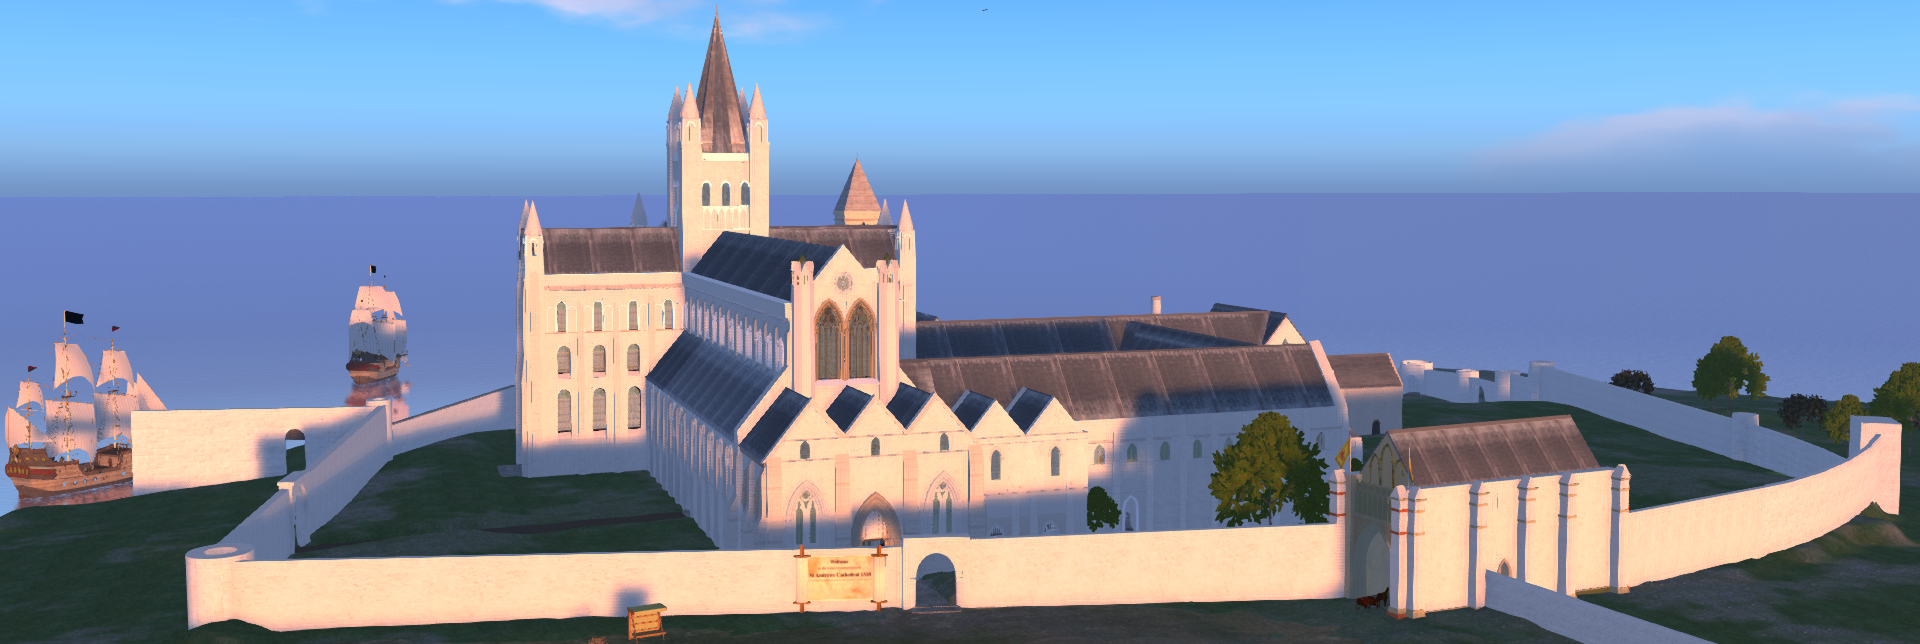
\includegraphics[width=\linewidth]{cathedral_reconstruction_side.png}
  \caption{St Andrews Cathedral recreation set on the sunny St Andrews day afternoon 1318, showing the West Gate in the foreground \& ships in the background.}
  \label{cathedral_reconstruction_side.png}
\end{figure}

%=====================

%~\cite{Kennedy2013} Canons \& Cathedrals

St Andrews Cathedral occupies a site used for worship since the 8th Century AD. Work on the Cathedral began around 1160 and was completed nearly 150 years later (the west fa\c{c}ade and parts of the nave collapsed in a storm around 1270). It was finally consecrated in 1318 four years after the battle of Bannockburn and in the presence of King Robert I of Scotland. St Andrews Cathedral was in its prime, the centre of Scotland’s religious life, its largest and most magnificent church. In 1378 the Cathedral suffered a significant fire prompting
a reworking of many of its features including the West and East End windows. Its presence was the catalyst for the foundation of a university at St Andrews in the early fifteenth century~\cite{Fawcett2011}, which remains an important seat of learning to this day. In 1561 following the Scottish reformation the Cathedral was abandoned by the Bishops and replaced by the parish church as the chief place of worship. The former headquarters of the Scottish Church was left to fall into ruin, with much of its stone being used in the construction of town dwellings.

During its time the Cathedral was central to Scottish personalities and history. St Andrews was the highest ranking Scottish see. The establishment of Augustinian Cannons followed by the initiation of
building work by Bishop Ernald reflected integration with the European church, economic dynamism and decline of the Celtic Church. The diocese funded Robert Bruce during the Wars of Independence. Its Bishop William de Lamberton contributed to the formulation of the Declaration of Arbroath, a central document in the formation of
Scottish Nationhood. Isabella, sister of Donnchadh IV, last Pictish Earl of Fife, crowned Bruce King. John Knox personally lead his congregation against the Cathedral’s finery and following the murder of Cardinal Beaton the first Scottish protestant congregation was established in the Bishop’s palace.

Important fragments of the remain. The east gable of the presbytery, where the relics of St Andrew were purported to be kept, along with the south wall of the nave, and the majestic West Entrance all point to the Cathedral’s former majesty. The cloister retains its ruined chapter house and stone-vaulted under crofts. Consequently, much evidence of the Cathedral’s form exists. A view from the nave looking towards the choir in figure \ref{cathedral_real_outside.jpg}.

%=====================

The OVW Group's reconstruction of St Andrews cathedral, as shown in figures \ref{cathedral_reconstruction_side.png} \& \ref{cathedral_reconstruction_above.jpg}, represents the site as it stood in 1318, the year of its consecration. This virtual reconstruction, presenting a historically accurate model of the cathedral as it stood at the peak of its former glory, is very large at over 400m by 600m \& spanning multiple storeys, featuring the cloisters as well as the Cannons' living quarters.

\TwoFig{cathedral_real_outside.jpg} {St Andrews cathedral today.} {cathedral_real_outside.jpg}
       {cathedral_reconstruction_above.jpg} {St Andrews cathedral reconstruction.} {cathedral_reconstruction_above.jpg}

%=========================================================================================================

\subsection{Experimental Implementation}

\textbf{***Go through Arduino sketch \& talk about things like magnetic declination, etc.}

%Magnetic declination information was entered into the HMC6343 for the position of the cathedral and the date of our experiments. The HMC6343's hard-iron offset calculation feature was used each time the hardware configuration was altered. The sampling frequency of the HMC6343 was set to its highest value of 10Hz. Orientation was set to `upright front' to match the physical orientation of the IC in the experiments.


%The MAX-6 was operated in `pedestrian' dynamic platform model, use of SBAS correction data was enabled and frequency of readings was set to the maximum of 5Hz.

For the purposes of testing VTW at the cathedral, a temporary server \& network setup was effected using a Lenovo ThinkPad X61s\thinkpadFootnote{} laptop computer to host the OpenSim server with a Linksys WRT54G\wrtFootnote{} wireless router powered from a 12V sealed lead-acid battery to provide wireless communication between the OpenSim server \& the WindPad over a much larger range than the laptop's internal wireless interface could provide. This setup is shown in use at the cathedral by figure \ref{pangolin_laptop_router_battery.jpg}, the architecture of this experimental implementation is shown by figure \ref{vtw_implementation.png} \& figure \ref{vtw_in_use.jpg} shows VTW in use at the cathedral.

\TwoFig{pangolin_laptop_router_battery.jpg} {OpenSim Server \& wireless AP.} {pangolin_laptop_router_battery.jpg}
       {vtw_in_use.jpg} {VTW at the cathedral.} {vtw_in_use.jpg}

\begin{figure}[h]
\centering
  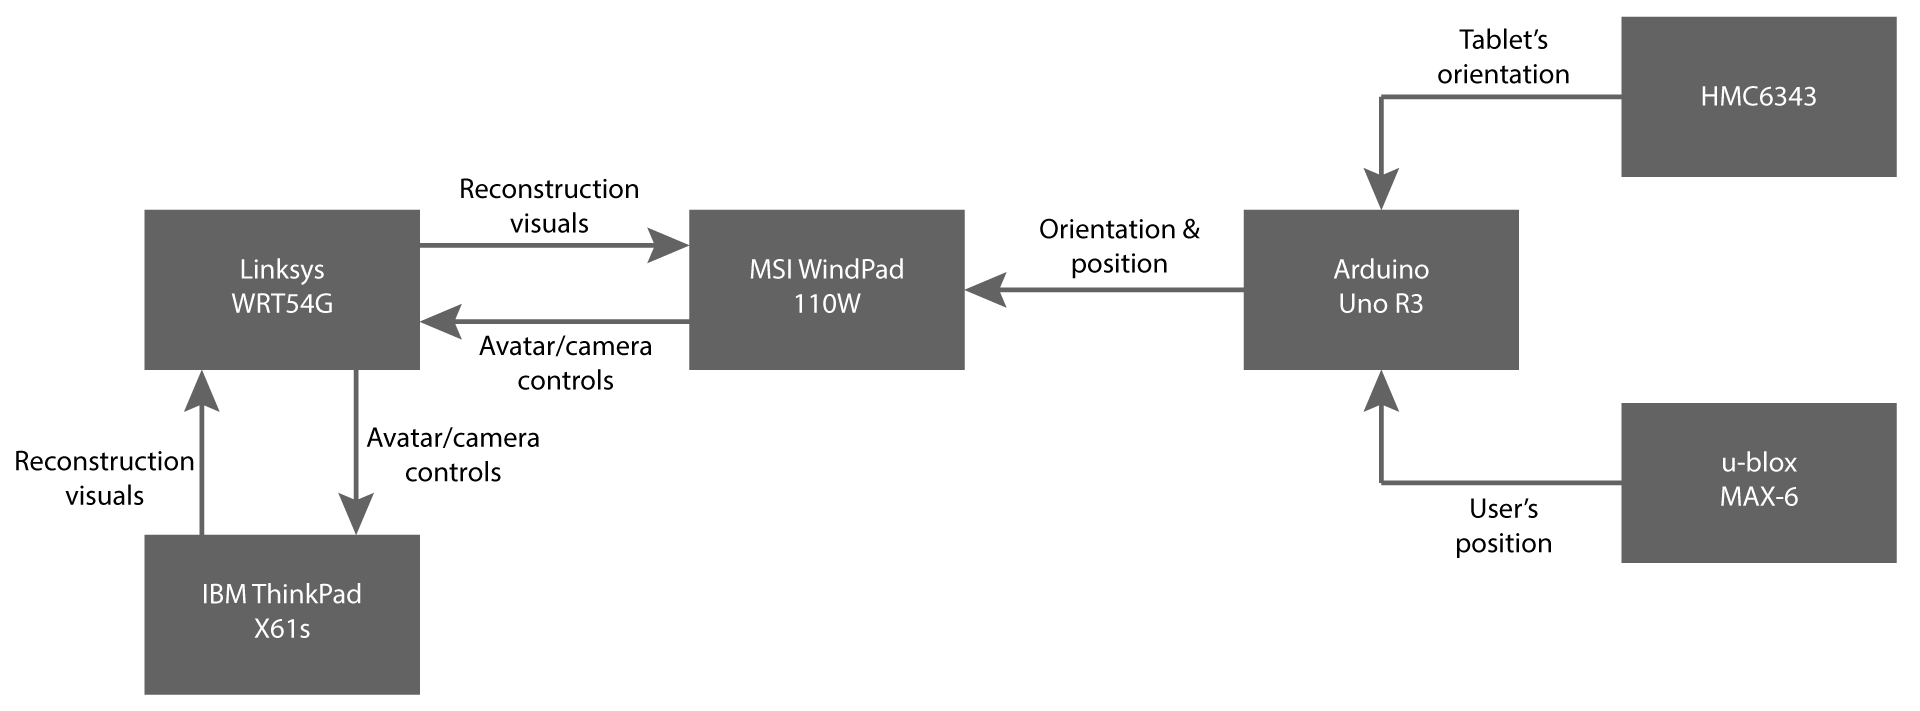
\includegraphics[width=\linewidth]{vtw_implementation.png}
  \caption{Implementation of VTW.}
  \label{vtw_implementation.png}
\end{figure}

%=========================================================================================================

\subsection{Real World Performance of VTW}

\newcommand{\ubloxcepFootnote}{\footnote{\url{https://u-blox.com/images/downloads/Product_Docs/MAX-6_ProductSummary_(GPS.G6-HW-10089).pdf}}}

\newcommand{\ucenterFootnote}{\footnote{\url{https://u-blox.com/en/evaluation-tools-a-software/u-center/u-center.html}}}

\newcommand{\htconesFootnote}{\footnote{\url{http://www.htc.com/uk/smartphones/htc-one-s/}}}

\newcommand{\snapdragonFootnote}{\footnote{\url{https://www.qualcomm.com/products/snapdragon/processors/s4-s1}}}

\newcommand{\mytracksFootnote}{\footnote{\url{https://play.google.com/store/apps/details?id=com.google.android.maps.mytracks&hl=en}}}

\newcommand{\hausdorffFootnote}{\footnote{\url{http://postgis.net/docs/ST_HausdorffDistance.html}}}

%=====================

The product summary for the MAX-6 claims accuracy of 2.5m Circular Error Probable (CEP) without SBAS corrections and 2m CEP with SBAS corrections \textit{``demonstrated with a good active antenna''}\ubloxcepFootnote{}. This means that, in an ideal situation with SBAS correction data available, there would be 50\% certainty that each position reported by the GPS receiver would be within 2m of its actual position. The SL-1202 antenna used is passive, however as the distance between antenna and the MAX-6 IC itself in the hardware application is only a few millimeters there would have been negligible benefit from using an active antenna. However whether the SL-1202 constitutes `good' for achieving the headlining performance characteristics of the MAX-6 is debatable as the definition of `good' was not provided in the product summary.

To determine the real world accuracy attainable with the MAX-6 outfitted with the SL-1202 in situations akin to those of the cultural heritage case study, a walking route around the St Andrews cathedral ruins, akin to the route that an individual visitor or school group might take, was planned and then walked with the MAX-6 connected to a laptop computer via an Arduino operating as a Universal Asynchronous Receiver/Transmitter (UART) feeding the raw NMEA messages into the u-center\ucenterFootnote{} GPS evaluation software version 7.0 which logged the messages for later evaluation. Simultaneously for comparative purposes a mid-range consumer Android smartphone was used to record the same track; a HTC One S\htconesFootnote{} containing a gpsOne Gen 8A solution within its Qualcomm Snapdragon S4 processor\snapdragonFootnote{} and using Google's My Tracks\mytracksFootnote{} app version 2.0.3 to record the data.

The three sets of positional data (planned route, MAX-6 recorded route and smartphone recorded route) were entered into a PostgreSQL database and the PostGIS database extender's \texttt{ST\_HausdorffDistance} algorithm\hausdorffFootnote{} was used to calculate the Hausdorff distances between the recorded routes and the planned route and between the recorded routes themselves. In this scenario, the Hausdorff distance represents the furthest distance needed to travel from any point on the route recorded by the GPS receiver to reach the nearest point on the planned route. Because of the substantially greater inaccuracies identified in the latter part of the recorded tracks, separate Hausdorff distances were calculated both for the complete tracks and also for truncated first and second sub-tracks.

%This ability to control navigation within the 3D virtual environment without explicit conscious input of keyboard/mouse/touch commands is integral to reducing the cognitive load required to maintain a presence within a virtual environment which is a key requirement for overcoming the vacancy problem and achieving successful mobile cross reality.

During the experiments the MAX-6 was unable to maintain reception of the additional correction data required for SBAS operation; when left stationary for several minutes reception was possible however subsequent movement of only a few meters at walking pace broke the connection. This reduced the theoretical maximum performance of the unit to 2.5m CEP, with observed performance being lower. Figure \ref{vtw_all_routes.png} depicts an aerial view of the St Andrews cathedral ruins; the blue line represents the planned route, red the route recorded by the MAX-6 receiver and green the route recorded by the smartphone for comparative purposes, both while walking the planned route.

\begin{figure}[h]
\centering
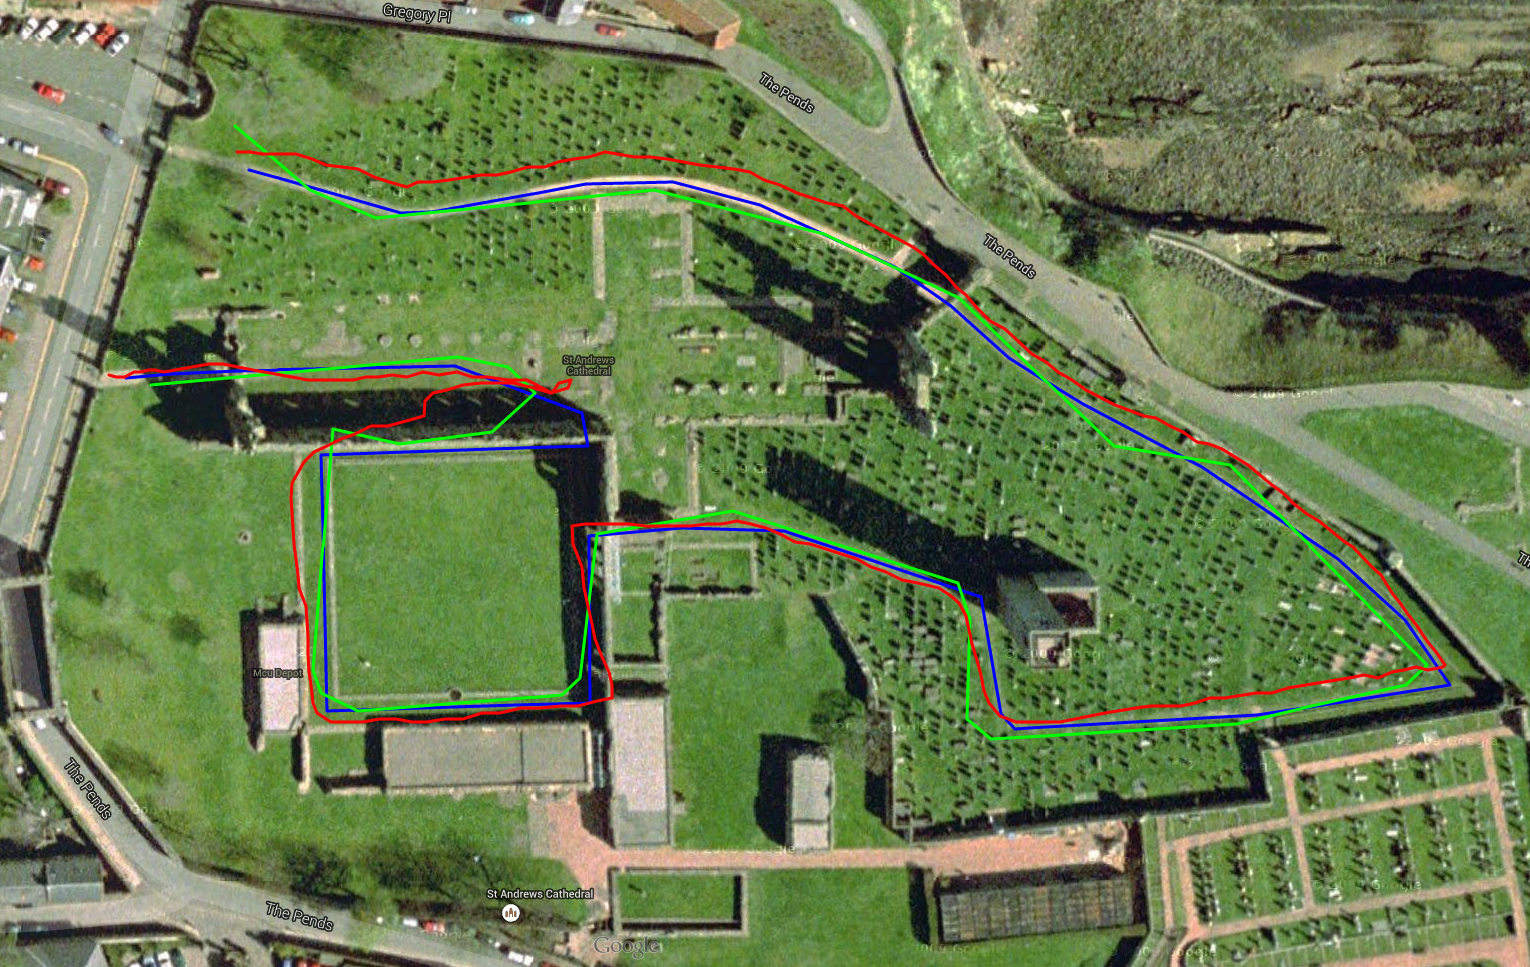
\includegraphics[width=0.8\textwidth]{vtw_all_routes.png}
\caption{Aerial view oriented North upward of the St Andrews cathedral ruins; the blue line represents the planned route, red the route recorded by the MAX-6 and green the route recorded by the smartphone whilst walking the planned route.}
\label{vtw_all_routes.png}
\end{figure}

The Hausdorff distance between the planned route and that recorded by the MAX-6 was $1.02e^{-04\circ}$. The `length' of a degree of latitude and a degree of longitude depends upon location upon the Earth; around the location of the St Andrews cathedral 1$^\circ$ of latitude is equivalent to 111347.95m and 1$^\circ$ of longitude to 61843.88m. Thus the Hausdorff distance of $1.02e^{-04\circ}$ can be visualized as $\pm11.3$m of North/South inaccuracy or $\pm6.3$m of East/West inaccuracy (or a combination of both N/S and E/W inaccuracy not exceeding a total displacement of $1.02e^{-04\circ}$ from the planned route).

The MAX-6 did achieve better performance than the smartphone, which recorded a Hausdorff distance of $1.33e^{-04\circ}$ ($\pm14.8$m N/S, $\pm8.2$m E/W). The Hausdorff distance between the routes logged by the MAX-6 and the smartphone was $1.14e^{-04\circ}$ ($\pm12.7$m N/S, $\pm7.0$m E/W), which represents a low correlation between the inaccuracies recorded by the two receivers even though they are of similar magnitudes from the planned route.

The maximum inaccuracies were recorded when walking along the South wall of the cathedral's nave. This wall is one of the most complete sections of the building with stonework reaching some 30ft above ground level (as can be seen in figure \ref{cathedral_real_outside.jpg}) and providing an effective obstruction to line-of-sight to half of the sky (and substantially impairing reception of signals from GPS satellites) when in close proximity to it. When considering just the sub-route shown in figure \ref{vtw_alll_routes_first_half.png}, which terminates before this wall begins to significantly obstruct view of the sky, the Hausdorff distances are notably smaller; the MAX-6 achieved a Hausdorff distance of $7.23e^{-05\circ}$ ($\pm8.05$m N/S, $\pm4.47$m E/W) throughout this sub-route, with the smartphone still behind with $8.99e^{-05\circ}$ ($\pm10.01$m N/S, $\pm5.56$m E/W). Again the Hausforff distance between the receivers showed low correlation between the inaccuracies, at $6.43e^{-05\circ}$ ($\pm7.12$m N/S, $\pm3.98$m E/W).
 
\begin{figure}[h]
\centering
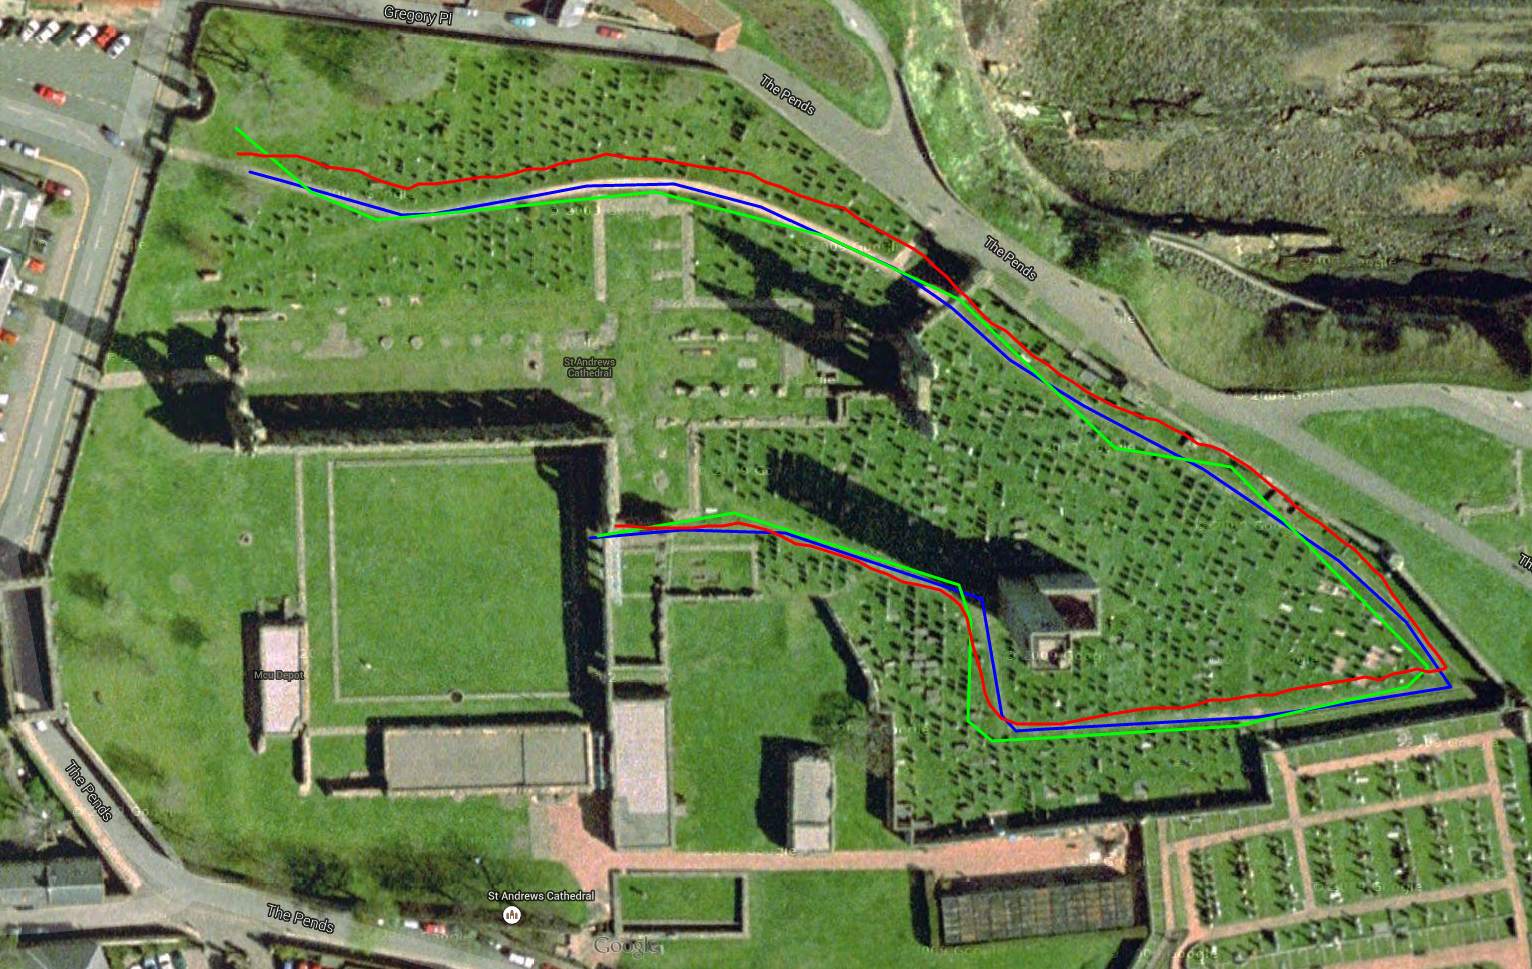
\includegraphics[width=0.8\textwidth]{vtw_alll_routes_first_half.png}
\caption{Aerial view oriented North upward of the St Andrews cathedral ruins; the blue line represents the first sub-route of the planned route, red the sub-route recorded by the MAX-6 and green the sub-route recorded by the smartphone whilst walking the first planned sub-route.}
\label{vtw_alll_routes_first_half.png}
\end{figure}

When analyzing the tracks in the vicinity of the nave (see figure \ref{vtw_all_routes_second_half.png}) it is shown that although the MAX-6 outperformed the smartphone in terms of Hausdorff distance this relationship can be considered misleading as the smartphone track corresponded more closely in shape to the planned route even if it did stray further at its extreme. The discrepancy in the behavior of the two receivers in this situation is attributed to different implementations of dead-reckoning functionality between the receivers. Dead-reckoning is the process used when a GPS receiver loses reception of location data from satellites and extrapolates its position based upon a combination of the last received position data and the velocity of travel at the time of receiving these data.
 
\begin{figure}[h]
\centering
\includegraphics[width=0.8\textwidth]{vtw_all_routes_second_half.png}
\caption{Aerial view oriented North upward of the St Andrews cathedral ruins; the blue line represents the second sub-route of the planned route, red the sub-route recorded by the MAX-6 and green the sub-route recorded by the smartphone whilst walking the second planned sub-route.}
\label{vtw_all_routes_second_half.png}
\end{figure}

VTW's camera control from orientation data does not have as stringent performance criteria as the movement control from position data. Unlike AR applications where sparse virtual content is superimposed upon a view of a real environment and the virtual objects must be placed accurately in order for the effect to work well, PR presents a complete virtual environment that is viewed `separately' or side-by-side with the real environment and thus discrepancies between orientation of real and virtual environments have a less detrimental effect to the experience. Although the accuracy of the camera control during the experiments was reported as being sufficient, the speed at which the camera orientation moved to match physical orientation was reported as being too slow, resulting in having to wait for the display to `catch up' to changes in orientation. This is attributed to the 10Hz sampling rate of the orientation sensors which, particularly after readings are combined for smoothing purposes to reduce jerky movement, resulted in too infrequent orientation updates. Frame rates within VTW whilst navigating the route averaged between 15 and 20 frames per second with the Second Life client's `quality and speed' slider set to the `low' position.

The style of explorative interaction with virtual content that this system employs is more resilient to input lag and low frame rates than other scenarios of interaction with virtual content such as fast paced competitive video games including First Person Shooters (FPS) [20], but overall user experience would nonetheless be improved by a faster sampling of orientation data and a higher frame rate. Additionally it should be noted that the cathedral reconstruction was created with relatively powerful desktop computers in mind as the primary deployment platform and has not been optimized for use on less powerful mobile platforms such as VTW. Performance of VTW on a less graphically complex OpenSim region that also depicts a reconstruction of a cultural heritage site, was better at 20 to 25 frames per second at the `low' position and between 15 and 20 frames per second at `high'.

%\begin{figure}[h]
%\centering
%\includegraphics[width=0.48\textwidth]{vtw_fps_plot_salt_pans.jpg}
%\caption{Plot of Pangolin's performance (measured in frames per second) against different graphical settings (selected via the `Quality and speed' slider of the viewer) in two positions within the Salt Pan 2 region.}
%\label{vtw_fps_plot_salt_pans.jpg}
%\end{figure}

%=========================================================================================================

\subsection{Performance Implications}

\textbf{***Talk about static modality being too similar to existing XR projects (\& mobile modality needs better positional tracking). Also mention how tablet isn't immersive enough \& HMD (with better trackig) is the next plausible step (eg next chapter!)?}

The positional accuracy of $1.02e^{-04\circ}$ attained by the MAX-6 is not sufficient for the style of interaction that VTW envisaged. This value, analogous to a combination of $\pm11.3$m of North/South inaccuracy or $\pm6.3$m of East/West inaccuracy, represents a constraint on the granularity of the content; it is the minimum distance required between any two points of interest for them to be correctly differentiated between. This value is too large to differentiate between, for example, two sides of a wall \& is likely to situate a user's virtual presence on the opposite side of a wall to their real presence, especially when that wall still exists in the real world to interfere with GPS reception, ruining the effect of being able to switch between real \& virtual stimuli. After experiencing VTW with, at times, theoretically as low as 2m CEP, an accuracy of around 1m CEP (analogous to $8.98e^{-06\circ}$ latitude or $1.62e^{-05\circ}$ longitude around the location of the St Andrews cathedral) is envisaged as the minimum for successful implementation of the VTW concept.

The accuracy of orientation tracking does not change with different positional accuracy and the accuracy attained in the experiments was sufficient for an acceptable user experience, however the experience would benefit greatly from better graphical quality and higher responsiveness to changes in user orientation. The immersiveness of a hand held tablet is also rather poor, which does not fit well with one of the major proposed benefits of the PR concept - the ability to produce immersive, atmospheric virtual visuals (especially when compared to paradigms such as AR which have established hand held implementations).

%=========================================================================================================

\section{Summary}

This chapter has introduced virtual heritage as a field in which the successful application of alternate reality techniques has a proven history \& to which the application of PR promises to be of further benefit. The Virtual Time Window project was introduced as an initial foray into the realm of applying PR to virtual heritage, making use of an x86 tablet computer imbued with position \& orientation sensing via GPS \& combined accelerometer/magnetometer, for PR exploration of outdoor cultural heritage sites \& their virtual reconstructions hosted upon an OpenSim framework. An implementation of this platform is presented, however real world experimentation revealed that the accuracy of positional tracking obtainable, even by discrete GPS receivers that outperform those mainstream receivers found in smartphones, is not sufficient for the envisaged style of interaction. Furthermore, the ability of a complete virtual environment presented on a small hand held display to provide a greater sense of immersion in a complete, atmospheric virtual environment was found to be lacking \& thus the pursuit of this modality of PR interaction was not continued.

%=========================================================================================================

% ======= ======= ======= ======= ======= ======= =======

\chapter{Mirrorshades - Development}
\graphicspath{ {05_mirrorshades_design_implementation/images/} }
\begin{quote}
	\textit{``A vacant-eyed clerk glanced up at me \ldots\ He was wearing a bifocal visor, which gave him a semitransparent view of the OASIS while also allowing him to see his real-world surroundings.''}%~\cite{Cline2012}
\end{quote}
\hfill \textit{Ready Player One, Ernest Cline}
\\
\\

%=========================================================================================================

\label{chapter-mirrorshades}

This chapter discusses the design and development of a parallel reality platform that combined a wide field of view (FOV), stereoscopic 3D, VR HMD modified with cameras for video see-through, with an indoor positioning system (IPS). This platform allows its user to observe and move around their real environment while imbued with the ability to alternatively view a complete immersive VR environment from the equivalent vantage point. Development of this platform enabled investigation of parallel reality in a manner that fully realised the envisaged experiential aspect of wholly switching between immersive real and virtual environments. The use of higher performance position and orientation tracking promised to allow for the freeform exploration scenario from section \ref{parallel-reality-in-virtual-heritage} to take place at closer ranges in smaller, indoor spaces and with sufficient accuracy to even experience aspects of the third detailed comparison scenario.

%Previous XR research approached the vacancy problem by integrating sensor/actuator networks into the environments, such that actions in one could manifest in the other, however direct visual engagement with the virtual environment was only possible from static interfaces at pre-determined locations within the real environment~\cite{Lifton2007a, Dublon2011}. The platform discussed in this document addresses this shortcoming by providing a mobile interface for visual engagement with both environments of a XR system, allowing the user to transition between viewing their real environment and a virtual environment at any time while maintaining the freedom to move around them, multiplexing visual stimuli from their real surroundings and from a parallel, virtual `mirror world'~\cite{Gelernter1993}.

%=========================================================================================================

%A second example of such a situation is found in the book \textit{Ready Player One}, in a scene in which the protagonist users the equivalent of an Internet cafe to access the \textit{OASIS};

%The OASIS is similar to Snow Crash's Metaverse; a fictional multi-user 3D environment with no enforced likeness to the real world, accessed via \textit{``a visor and a pair of haptic gloves''}. The bifocal visor allows this character to switch his attention between the virtual environment of the OASIS and his real surroundings in the Internet cafe.

%=========================================================================================================

%With a display technology such as an immersive VR HMD however, 

\section{Overview}
The development of the VTW platform as a preliminary foray into applying the concept of parallel reality to the field of cultural heritage performed sufficiently to implement the static viewpoint scenario described in section \ref{parallel-reality-in-virtual-heritage}, wherein the viewpoints are spaced further apart than the worst case accuracy of the GPS solution, and to partly explore the freeform exploration scenario for expansive outdoor cultural heritage sites, in which visitors view artefacts within the environments from some distance from where the inaccuracy of positioning is not apparent.

To continue the investigation of parallel reality, once again using cultural heritage as a real world case study, the platform described in this chapter aimed to allow the investigation of the use of parallel reality at indoor cultural heritage sites. This allowed the use of an IPS to track the user's position, which promised greater accuracy than even SBAS enhanced GPS did outdoors, allowing for the full freeform exploration scenario to be explored, even in much less expansive sites, and even for aspects of the third scenario with detailed comparison to be experienced. Furthermore the use of a HMD capable of producing stereoscopic 3D visuals that completely fill the user's view, in place of a tablet, allowed the investigation of parallel reality to extend to systems that present a completely immersive virtual experience instead of a `window' into the virtual, realising the true essence of the envisioned experiential aspect of parallel reality that VTW did not provide. Whilst VTW presented the user with a `screen' into the virtual, around which they could still perceive their real environment, with the HMD of this subsequent platform \textit{``there is practically no screen''} as it \textit{``totally covered by our field of view, vanishes''}~\cite{Tzortzaki2002}.

%=========================================================================================================

\section{The Mirrorshades Platform}
\label{the-mirrorshades-platform}
Figure \ref{systemarchitecture} presents a high level architectural overview of the Mirrorshades\footnote{\textbf{Mirrorshades: The Cyberpunk Anthology} (1986) is a defining cyberpunk short story collection edited by Bruce Sterling, who explains how mirrored sunglasses became a literary badge or `totem' for the cyberpunk movement whose fiction has frequently involved immersive multi-user virtual environments and HMDs.} parallel reality platform while figure \ref{participant-f-5.jpg} shows its implementation. Mirrorshades allows its user to observe and move around their real environment (RW) whilst wearing a stereoscopic 3D HMD, with their position and gaze tracked by an IPS and the HMD's head tracker, switching between viewing RW visual stimuli provided by cameras mounted to the HMD and immersive VR visual stimuli from the equivalent vantage point of the reconstruction as tracked by the IPS. A controller held by the user is used to control these switches between RW and VR. The mobile client that produces the graphical content delivered to the HMD is carried about the person in a bag/satchel.

\begin{figure}[h]
	\begin{center}
		\includegraphics[width=.5\linewidth]{system-architecture.png}
		\caption{High level overview of the Mirrorshades parallel reality platform.}
		\label{systemarchitecture}
	\end{center}
\end{figure}

\begin{figure}[h]
	\begin{center}
		\includegraphics[width=\linewidth]{participant-f-5.jpg}
		\caption{The Mirrorshades parallel reality platform.}
		\label{participant-f-5.jpg}
	\end{center}
\end{figure}

Emphasis should be placed on the fact that the two views, RW and VR, through the function of IPS and head tracking combined with the spatial equivalence of the constituent environments, represent equivalent vantage points within the two environments, differentiating the modality of interaction from the visual perception exchange systems exhibited in an Istanbul church by Mathieu Briand, which at first glance might have seemed to provide a similar modality at least in terms of the hardware employed and the heritage scenario.

\begin{quote}
	\textit{``In an earlier version, set in the Hagia Eirene church in Istanbul, visitors wearing a wireless headgear viewing device could press a button to exchange the image on the screen with that of another of the six headgear cameras, revealing whatever it was pointing at. Visitors were fascinated by the dynamic visual transformations, such as the way the brightly painted floor could suddenly be replaced by the church dome as they wandered around the space.''}~\cite{Jones2006}
\end{quote}

Likewise the modality of interaction provided by the Mirrorshades platform distances itself from that of Briand's later experiments into `controlled schizophrenia' in which displacement of body and vision were intentional, as the different views that a user of the Mirrorshades platform switches between are inherently the same `place' as seen from the same vantage point.

\begin{quote}
	\textit{``The audience members wear helmets that incorporate a camera, goggle-style compact monitor, and headphones. The audience members may also carry a connector that can be plugged and unplugged from the nine sockets placed around the museum, in order to exchange audiovisual experiences with others.}

	\textit{When a connector is not plugged into a socket, one sees the environment through his/her own camera. In other words, one walks around seeing the surrounding environment through his goggle monitor. When the connector is plugged into a socket on the wall, the person sees the view taken by one of the three cameras installed in the building, or taken by another camera worn by another audience member whose camera is also connected to a socket.''}~\cite{Jones2006}
\end{quote}

%=========================================================================================================

\subsection{St Salvator's Chapel}

The location elected for application of the Mirrorshades platform was St Salvator's chapel in St Andrews. Founded in 1450 but internally stripped of its medieval fittings during the Protestant Reformation (1517 - 1648) the chapel looks markedly different today than it did upon its completion. An existing virtual reconstruction of the chapel as it stood in the period 1450-1460, created by the OVW group, and the marked differences between the internal appearance of the reconstruction and the present day building (including the replacement of the original stone roof with a wooden one and drastically different dividing of the internal space) made the chapel an ideal candidate within the context of cultural heritage for the Mirrorshades parallel reality system to be deployed. The magnitude of the changes between the chapel's original state and how it stands today means that augmented reality would not in fact be able to present a faithful image of how the chapel originally looked, but would need to be combined with substantial application of diminished reality to remove present day features that were not there in the past. For example, when in proximity to the rood screen in its new position (discussed beneath), removing it would require replacing almost the entire viewport with augmented or diminished visuals.

\TwoFig{sallies-vrst/sallies-quad-real.jpg}{St Salvator's chapel today.}{sallies-quad-real.jpg}
       {sallies-vrst/sallies-quad-virtual.png}{St Salvator's chapel reconstruction.}{sallies-quad-virtual.png}
       
The chapel was of the greatest significance for the new architectural ideas that it introduced into Scotland, at a time when Scotland was particularly open to external artistic influences. However although the shell of the chapel survives and remains in use, it has lost its vault, its window tracery and its liturgical furnishings; it now requires specialist skills to appreciate the quality of its original state. As with other reconstructions from the OVW group, the virtual St Salvator's chapel was a product of a collaboration between architectural, art history and computer science scholarship. On the combined evidence of a highly detailed late medieval inventory and of the architecture itself, it has been possible to show how the chapel was furnished internally with altars, choir stalls, lecterns, screens, stained glass and wall paintings. The architectural, liturgical and spatial analysis allows our understanding of the history of the Chapel as a living building to be enormously enhanced by experiencing the building in its original context.

\TwoFig{sallies-vrst/sallies-real-toward-altar.jpg}{St Salvator's chapel looking East, present day.}{sallies-real-toward-altar.jpg}
       {sallies-vrst/sallies-virtual-toward-altar.png}{St Salvator's chapel looking East, reconstruction.}{sallies-virtual-toward-altar.png}

The chapel is an aisle-less rectangle with a three-sided east apse. Deeply projecting three-stage buttresses define the bays, which are now capped by pinnacles of 1861-2. The windows which occupy the full space available between the buttresses no longer reflect their original forms. The main entrance to the chapel was originally through a doorway in the second bay from the west of the south flank, which is covered by a vaulted porch between the buttresses. Two doorways on the north side presumably opened into a lost sacristy and treasury range.

The interior of the chapel is known to have been covered by a stone vault, which is assumed to have been of pointed barrel form with a decorative pattern of ribs, like the small vault over the south porch. The interior is now covered by an inappropriate timber roof.

\TwoFig{sallies-vrst/sallies-real-from-altar.jpg}{St Salvator's chapel looking West, present day.}{sallies-real-from-altar.jpg}
       {sallies-vrst/sallies-virtual-from-altar.png}{St Salvator's chapel looking West, reconstruction (note closer position of rood screen).}{sallies-virtual-from-altar.png}

St Salvator's chapel is considered the first Scottish example of a church planned with an aisle-less rectangular main body terminating in a polygonal eastern apse, a type that was to have a long future for a range of Scottish church types. Such chapels were common in university colleges in France and since Bishop Kennedy had a highly placed kinsman in the university of Paris and drew many ideas for the organisation of his college from that university's constitution, it is reasonable to assume that he also drew some of his ideas for the architecture of his chapel from there. On this basis, St Salvator's must be seen as an outstandingly important channel for the introduction into Scotland of new architectural ideas from France. The new architecture made a significant statement in its Scottish context. 

The reconstruction of the chapel involved both the mental reconstruction of modified and lost features, and the establishment of the range of ways in which buildings that represent a spirituality alien to modern students were intended to function. As such it offers an invaluable academic discipline for those involved in the reconstruction, providing eminently practical ways of testing theories and assumptions. The development of a parallel reality system which enables comparison between the real and virtual chapel in the same time and place aimed to further enhance the value of the reconstruction.

%=========================================================================================================

\section{Virtual Reality HMDs}
The concept of virtual reality and the associated HMDs that provide wide field of view, stereoscopic 3D graphics coupled with head tracking is currently experiencing a resurgence of interest and investment, thanks largely to the advent of Oculus\footnote{\url{https://www.oculus.com/}} and their Rift platform\footnote{\url{https://www.oculus.com/rift/}}. Whilst the first head mounted computer display was created in the late 1960s by Ivan Sutherland~\cite{Rheingold1992}, it was not until the late 1980s and early 1990s that VR began to be promoted as a consumer platform. Unfortunately both hardware and software were not ready for consumer adoption at this time and these systems failed to live up to the substantial hype of being a \textit{``revolutionary technology''} which promised to \textit{``transform society''} (figure \ref{rheingold-virtual-reality.jpg}), resulting in the VR bubble bursting.

\begin{figure}[h]
	\begin{center}
		\includegraphics[width=0.4\textwidth]{rheingold-virtual-reality.jpg}
		\caption{Howard Rheingold's 1992 bestseller \textit{Virtual Reality}.}
		\label{rheingold-virtual-reality.jpg}
	\end{center}
\end{figure}

Decades after this initial disappointment with consumer centric VR, Oculus now looks set to finally begin realising a successful consumer VR platform thanks largely to the substantial advances in display technologies made during the past decade driven primarily by the explosive popularity of smartphones and tablets. Pre-Oculus HMDs predominantly made use of two separate microdisplays, one for each eye; Sutherland's original `Sword of Damocles' made use of two tiny CRT screens, whilst later HMDs made use of two OLED microdisplays. As the number of market applications for microdisplay technology was (\& continues to be) relatively small, there are limited microdisplay models to chose between and they command high price points when considering integration into consumer products.

Oculus have taken a different approach for their Rift Developer Kit HMDs. Instead of using two small displays, one for each eye, they use a single larger display upon which two separate images are rendered, side-by-side. This approach has two distinct advantages compared to prior dual microdisplay techniques. Firstly the complexity of the device is reduced, which positively impacts price, ease of integration and content development methodologies. Secondly the cost of a single display in the 5"-7" range is drastically lower than the cost of a pair of microdisplays, thanks to the surging popularity of smartphones and tablet computers in this size range. By making use of readily available displays intended for the smartphone/tablet market, Oculus were able to bring their first Development Kit (DK1) to market for researchers and enthusiasts at a price of only \$300, while still providing substantially wider FOV than the vast majority of existing HMDs - even those commanding substantially higher price points.

For comparison, examples of consumer-grade commercial HMDs that use the twin OLED microdisplay approach, the Sony HMZ-T1 which launched with a price of \textyen60,000 (\$800 at exchange rates of the time) and its successor the HMZ-T2 which launched with a price of \textyen70,000 (\$900 at exchange rates of the time), provide $45$\textdegree\ horizontal FOV/$51.6$\textdegree\ diagonal and no head tracking (intended primarily as a personal 3D cinema experience). Oculus' DK1 provides more than $90$\textdegree\ horizontal and $110$\textdegree\ diagonal FOV and integrates a head tracking solution operating at a rate of 1kHz and providing best in class accuracy. Combined with advances in both hardware and software tasked with producing 3D graphics, the user experience of Oculus' HMD offerings is promising to finally deliver on the VR hype of the 90s.

The March 2014 acquisition of Oculus by Facebook\footnote{\url{https://www.facebook.com/zuck/posts/10101319050523971}} for \$2 billion\footnote{\url{http://www.theguardian.com/technology/2014/jul/22/facebook-oculus-rift-acquisition-virtual-reality}} and Oculus partnership with Samsung, one of the world's leading display manufacturers and which has already led to the release of an innovative VR HMD that makes use of an existing smartphone as its display\footnote{\url{https://www.oculus.com/gear-vr/}}, lends hope that this wave of VR excitement will be met with success where its hype-laden 90s counterpart was met with failure.

%\textbf{***Maybe talk about what other HMDs there were actually available to me on the market? Vuzix 1200/900/whatever?}

%take bits from that youtube video from Samsung developers?

%=========================================================================================================

\subsection{The Oculus Rift DK1 and Unity Game Engine}

The OVW group took delivery of an Oculus Rift DK1 from the first batch of units shipped to the EU in August 2013. The immersive experience of using the DK1, thanks to its wide FOV, fast and accurate head tracking, stereoscopic 3D and novelty compared to traditional 2D displays, presented a markedly different modality of interaction with virtual content than the 10'' display of the tablet used by VTW and by filling the user's entire field of view with whatever visuals are displayed upon its screen, the Rift allowed for investigation of the true essence of the experiential aspect of switching between real and virtual environments that parallel reality concept envisaged (see section \ref{real-world-experience-of-vtw}).

At this early stage after the DK1's release, the best supported software platform in terms of API provision and integration was the Unity game engine. After experience with modifying the Second Life client as part of the VTW project, it was decided best to convert the OVW group's OpenSim model of St Salvator's chapel into a Unity compatible format rather than embarking upon further modification to the Second Life client to support the DK1. Since the development of VTW the OVW group successfully engineered an automated process for converting OpenSim content into Unity compatible content, allowing the group's existing content to be deployed within Unity executables.

One deciding factor in opting to convert OpenSim content to Unity rather than use the content in its original OpenSim setting was the more stringent performance requirements for an enjoyable VR HMD experience compared to those of a traditional desktop/handhend display experience. When using a HMD such as the DK1, a high and smooth framerate is required to avoid a kind of motion sickness referred to as `simulator sickness'. Oculus' official guidelines are for Rift applications to \textit{``run at a frame rate equal to or greater than the Rift display refresh rate''}\footnote{\url{http://static.oculus.com/sdk-downloads/documents/Oculus_Best_Practices_Guide.pdf}} which in the case of the DK1 is 60Hz. Due to the possibly ephemeral nature of Second Life/OpenSim content where users are free to create, modify and destroy content in real time, Second Life as a 3D platform suffers in terms of performance compared to game engines such as Unity due to not being able to exploit techniques such as occlusion culling~\cite{willmott:largecomplex} which require an offline processing phase that depends upon environmental content remaining unchanged throughout deployment. The OVW group's experience in presenting Second Life/OpenSim content on a range of different hardware did not point to good odds of managing to render the St Salvator's chapel scene at close to 60fps, especially considering the overhead introduced by stereoscopic rendering even where the total resolution of the two side-by-side images is no greater than the single equivalent monoscopic image. As Mirrorshades is a mobile application and the computer producing the visuals was to be carried by the user, the hardware specification of this client were limited compared to those that the group had used in alternative static deployments.

%=========================================================================================================

\subsection{Modifying the DK1 for Video See-Through}
\label{modifying-dk1}
The Oculus Rift DK1 covers the user's entire field of view, such that they cannot see any of their real world surroundings whilst wearing it, and it does not feature any camera provision to allow a mediated view of the real world to be presented to them. As such it was necessary to modify the DK1 to imbue it with such video see-through capability for use as a component of the Mirrorshades parallel reality platform. When choosing cameras for this task there were several desired features:
\begin{itemize}
	\item Resolution and refresh rate that match (or exceed) those of the DK1's display.
	\item Sensor aspect ratio that matches that of each half of the DK1's display.
	\item Lens focal length and sensor dimensions that provide wide FOV (ideally matching the FOV of the DK1).
	\item Ease of integration with the Unity platform.
	\item Price realistic for a virtual heritage deployment.
\end{itemize}

The \$300 price tag of the DK1 and the low price of consumer webcams for computer and console use met with the budgetary requirement of the video see-through solution. The PS3 Eye camera met most of the technical requirements and has a history of use in research scenarios as part of the PS Move motion sensing platform (see section \ref{psmove}). While its resolution of 640x480 pixels does not meet each half of the DK1's display at 640x800 pixels, unusually for a USB camera it is capable of running at 60fps - the refresh rate of the DK1. The aspect ratio of the 640x480 sensor is 4:3, which although not identical to the 5:4 aspect ratio of each eye's 640x800 half of the DK1 screen, is closer than the 16:10 or 16:9 aspect ratio of a `widescreen' camera sensor. Furthermore once dismantled to its bare PCB it features mounting holes for a standard S-mount (M12x0.5mm) lens mount commonly used for CCTV cameras, allowing alternative focal length lenses to be easily fitted.

An early test with the PS3 Eye and the DK1 (a video of this test is available to view online\footnote{\url{https://www.youtube.com/watch?v=tS0FGZxQzCU}}) was performed by simply attaching a single unmodified PS3 Eye camera to the top of the DK1 (figure \ref{rift-pseye-ziptied.jpg}) with its stock lens set to its `wide' setting (75\textdegree, presumably diagonal, FOV\footnote{\url{http://uk.playstation.com/media/247868/7010571 PS3 Eye Web_GB.pdf}}). This test explored the suitability of Unity's \texttt{WebCamTexture}\footnote{\url{http://docs.unity3d.com/ScriptReference/WebCamTexture.html}} feature for integrating the stream from a USB camera into a 3D application. For this test the mediated RW video stream was rendered to a small `floating' window that moved with the user's head (figure \ref{floating-webcam-window.png}) allowing the user to perceive both environments simultaneously within the same viewport in a manner similar to VTW but in reverse - the virtual environment filling most of the viewport and the real environment as a smaller window in the periphery. Subsequently the camera streams were changed so as to render to the full expanse of the DK1's display, to better realise the switching experiential vision of parallel reality

\TwoFig{rift-pseye-ziptied.jpg}{Oculus Rift DK1 with PS3 Eye.}{rift-pseye-ziptied.jpg}
       {floating-webcam-window.png}{`Floating' window video see-through in Unity.}{floating-webcam-window.png}

A pair of PS3 Eye cameras were dismantled, their outer plastic housing removed, stock lenses removed and S-mount lens mounts fitted. Ideally the lenses used would provide the same FOV that the Rift itself is capable of displaying, such that the mediate RW streams from the cameras could be displayed at the full size of the Rift and `match' the FOV of whatever virtual content was alternatively displayed. However there is a trade off with lenses between focal length and distortion: shorter focal lengths mean a wider FOV, however they also introduce more distortion which is not necessarily corrected by the shader that the Rift uses to compensate for the distortion of its own plastic lenses through which its display viewed.

The PS3 Eye camera has a `1/4'' type' sensor but this classification is only an indication of its true dimensions\footnote{\url{http://www.dpreview.com/glossary/camera-system/sensor-sizes}}. As Sony has not published the actual dimensions of the sensor we adopted the typical 1/4'' type dimensions\footnote{\url{http://www.photoreview.com.au/tips/buying/unravelling-sensor-sizes}} of 4.5mm diagonal, 3.6mm horizontal, 2.7mm vertical for calculating FOV estimations. Table \ref{fov-table} gives the diagonal, horizontal and vertical FOV of the shortest focal length S-mount lenses readily available. Empirical accounts of very short focal length S-mount lenses mounted to the PS3 Eye camera indicated that the distortion becomes very high beneath 2.1mm\footnote{\url{http://peauproductions.com/store/index.php?main_page=index&cPath=26_4}}. Whilst 1.7mm lenses would provide almost identical FOV to the Rift's display (105.9\textdegree\ diagonal for the cameras, 110\textdegree\ diagonal for the Rift) the amount of distortion introduced would likely be of such an extent that the experience of viewing the mediate RW environment would be degraded more by distortion than by the limited/non-matching FOV provided by longer focal length lenses.

\begin{table}
\begin{center}
\begin{tabularx}{\textwidth}{c *{4}{>{\centering\arraybackslash}X}}
\toprule
\textbf{Focal length (mm)} & \textbf{Diagonal FOV (\textdegree)} & \textbf{Horizontal FOV (\textdegree)} & \textbf{Vertical FOV (\textdegree)} \\
\midrule
2.5mm & 84    & 71.5 & 56.7 \\
2.1mm & 93.9  & 81.2 & 65.5 \\
2.0mm & 96.7  & 84   & 68 \\
1.9mm & 99.6  & 86.9 & 70.8 \\
1.8mm & 102.7 & 90   & 73.7 \\
1.7mm & 105.9 & 93.3 & 76.9 \\

\bottomrule

\end{tabularx}
\caption{FOV of various focal length lenses resolving onto a 1/4'' type sensor.}
\label{fov-table}
\end{center}
\end{table}

However using a lens with a focal length short enough to provide a FOV as wide as the Rift was discovered to not be strictly necessary, as when wearing the Rift the edges of the image presented to each eye are not always visible to the user. This is especially true where the Rift's adjustable eye relief is set such that it sits at its furthest position. Such an adjustment is actually prudent for user study conditions, as using the Rift at its maximum eye relief ensures the best compatibility and comfort with users and also removes a variable between users that would be introduced if each were permitted to chose the relief themselves. Thus the choice of lens could be dictated by identifying the FOV required to fill the portion of the Rift's images that were visible when the eye relief was set to its maximal position, rather than by matching the Rift's overall FOV. This allowed the use of lenses with focal length long enough that the distortion they introduced was not so bad as to require a separate correction phase in software rendering.

Experiments revealed that with the DK1 set to its maximum relief, the area of the images visible to the user was wider than that provided by 2.5mm lenses (84\textdegree\ diagonal) when scaled correctly and narrower than that provided by 2.1mm lenses (93.9\textdegree\ diagonal) when scaled correctly. With no availability of lenses with a focal length between 2.5mm and 2.1mm, the 2.1mm focal length was adopted. Figure \ref{lens-comparison-on-ps3eye-pcb.jpg} shows the 2.5mm lens (right) and 2.1mm lens (left) mounted to the PS3 Eye PCBs via S-mount lens mounts, while figure \ref{fov-comparison-1.png} shows the FOV of the selected 2.1mm lenses scaled correctly upon the wider FOV of the DK1's images showing a scene within St Salvator's chapel.

\TwoFig{rift-clips-cameras/lens-comparison-on-ps3eye-pcb.jpg}{S-mount lenses on PS3 Eye camera PCBs.}{lens-comparison-on-ps3eye-pcb.jpg}
       {fov-comparison-1.png}{FOV comparison between DK1 and 2.1mm lenses.}{fov-comparison-1.png}

%{fov-comparison-2.png}{}{fov-comparison-2.png}

The PS3 Eye cameras were mounted to the DK1 by modifying the 3D printable sensor mount design released by the University of Southern California Institute for Creative Technologies\footnote{\url{http://projects.ict.usc.edu/mxr/diy/oculus-sensor-mount/}}. The modified mount comprised a base piece (figure \ref{clips.jpg}) that clipped securely over the front of the DK1 and a slotted plate (figure \ref{clips-hori-plate.jpg}) onto which the PS3 Eye cameras were mounted. These parts were 3D printed using a MakerBot Replicator 2X\footnote{\url{http://store.makerbot.com/replicator2x}} and combined using epoxy resin. The combination is shown attached to the DK1 in figure \ref{hori-1.jpg}. The slots in the slotted plate were spaced to match the mounting holes of the PS3 Eye PCB, such that the cameras could be attached by metal stand-offs (figure \ref{hori-2.jpg}) allowing horizontal adjustment to alter the distance between them to account for different interpupillary distances. Figure \ref{hori-3.jpg} shows how one camera was mounted `upside down' to allow enough clearance between the PCBs to accommodate small interpuillary distances.

\begin{figure}[h]
    \centering
    \begin{minipage}{.32\textwidth}
        \centering
        \includegraphics[width=\textwidth]{rift-clips-cameras/clips.jpg}
        \caption{Camera mount base.}
        \label{clips.jpg}
    \end{minipage}%
    \hspace{.01\textwidth}
    \begin{minipage}{0.32\textwidth}
        \centering
        \includegraphics[width=\textwidth]{rift-clips-cameras/clips-hori-plate.jpg}
        \caption{Camera mount slotted plate.}
        \label{clips-hori-plate.jpg}
    \end{minipage}%
    \hspace{.01\textwidth}
    \begin{minipage}{0.32\textwidth}
        \centering
        \includegraphics[width=\textwidth]{rift-clips-cameras/hori-1.jpg}
        \caption{Camera mount attached to DK1.}
        \label{hori-1.jpg}
    \end{minipage}
\end{figure}

\TwoFig{rift-clips-cameras/hori-2.jpg}{Cameras mounted using stand-offs.}{hori-2.jpg}
       {rift-clips-cameras/hori-3.jpg}{Two PS3 Eye cameras mounted on DK1.}{hori-3.jpg}

An oversight in the design of the camera mounts was realised when William Steptoe subsequently released details of his `AR Rift' project~\cite{Steptoe2014}. Although the DK1's overall screen has a resolution of 1280x800 in a landscape 16:10 aspect ratio, each half of this screen as presented individually to each eye has a resolution of 640x800 in a portrait 4:5 aspect ratio. Thus to best match the aspect ratio of a 4:3 camera sensor such as that of the PS3 Eye to each half of the DK1's screen, that camera should be oriented in a portrait orientation rather than the landscape orientation that had been employed thus far by the Mirrorshades platform with the PS3 Eye cameras. New mounting hardware was designed and printed by further modification of the USC's original 3D designs for vertical mounting of the PS3 Eye cameras. This new design is shown in figure \ref{clips-vert.jpg} (the recessed section in the centre of the clip allows for the heads of bolts to clear the front of the DK1) and the assembled units are shown attached to the DK1 in figure \ref{vert-6.jpg}. The files for printing both versions of the camera mounts are available online\footnote{\url{https://github.com/CJ-Davies/Oculus-Rift-DK1-camera-mounts}}. Additionally the metal stand-offs that had been used to mount the camera PCBs to the clips (see figure \ref{vert-1.jpg}) were replaced with a combination of rubber washers and threaded bolts (see figure \ref{vert-4.jpg}) both to reduce the discrepancy in the mediated RW images caused by the distance between the camera sensors and the user's eyes (by reducing this distance) and to allow for finer alteration of the orientation of the cameras.

\TwoFig{rift-clips-cameras/clips-vert.jpg}{Updated camera mount.}{clips-vert.jpg}
       {rift-clips-cameras/vert-6.jpg}{PS3 Eye cameras using updated mounts.}{vert-6.jpg}

\TwoFig{rift-clips-cameras/vert-1.jpg}{Updated camera mount with stand-offs.}{vert-1.jpg}
       {rift-clips-cameras/vert-4.jpg}{Updated camera mount with rubber washers.}{vert-4.jpg}

Although the initial integration test with a single PS3 Eye camera revealed its easy accessibility within Unity, using two PS3 Eye cameras proved temperamental. Unity's \texttt{WebCamTexture} support identifies webcams via their `name' as provided by their driver. In the case of the PS3 Eye using the driver provided by Code Laboratories\footnote{\url{https://codelaboratories.com/products/eye/driver/}} (this third party driver was required as no official Windows driver is available from Sony, as the PS3 Eye was only marketed for use with the PS3 console) an issue arose where both cameras presented the same name to Unity and the second camera overwrote the reference to the first, only allowing access to a single camera. Figure \ref{ps3-eye-unity-overwrite.png} shows this issue, that whilst Windows' device manager successfully identified both cameras independently, Unity's \path{WebCamTexture.devices()} function returned a reference to only one (the \texttt{BisonCam, NB Pro} entry is the laptop's internal webcam). A partial solution to this issue was presented by a community provided Unity package\footnote{\url{http://tips.hecomi.com/entry/20130731/1375279561} (Japanese)} which allowed the setup up to be successfully tested within a departmental building, a video of which is available to view online\footnote{\url{https://www.youtube.com/watch?v=oy5NqqDtkJ4}}.

\begin{figure}[h]
	\begin{center}
		\includegraphics[width=.8\linewidth]{ps3-eye-unity-overwrite.png}
		\caption{Unity failing to instantiate references to multiple PS3 Eye cameras.}
		\label{ps3-eye-unity-overwrite.png}
	\end{center}
\end{figure}

Unfortunately this naming solution was temperamental at best and two camera compatibility was frequently lost, so the PS3 Eye cameras were scrapped. Using Steptoe's project as a guide, a pair of Logitech C310\footnote{\url{http://www.logitech.com/en-gb/product/hd-webcam-c310}} cameras were sourced. Whilst the refresh rate of the C310 is only 30Hz, half that of the PS3 Eye, it supports a resolution of 1280x960 which is higher than that of the PS3 Eye and of each half of the DK1's display. The switch from the PS3 Eye cameras to the C310 represented a sacrifice in terms of framerate but a gain in terms of resolution. Empirically the increase in resolution was indiscernible, likely due to the effect of the DK1's optics in reducing the visual acuity of its display, whilst the reduction in framerate was noticeable. However the reliable operation of the C310 made them the superior option compared to the temperamental status of the PS3 Eye, which would have made it impossible to perform user studies due to unpredictable failures.

The C310 cameras received the same attention as the PS3 Eye cameras: they were dismantled and outfitted with S-mount lens mounts. As the sensor in the C310 is also of the 1/4" type the FOV provided by the 2.1mm lenses on the C310 cameras is comparable to that of the same lenses mounted to the PS3 Eye cameras. Due to the lack of mounting holes present on the C310 PCB they were set into a thin sheet of thermoplastic (figure \ref{thermoplastic.jpg}) which was then attached to the 3D printed clips with the same rubber washer and threaded bolt arrangement as the PS3 Eye cameras. The assembled DK1 + dual C310 solution is shown by figures \ref{vert-7.jpg} (3/4 view), \ref{middle.jpg} (profile view) and \ref{right.jpg} (detail view).

\TwoFig{rift-clips-cameras/thermoplastic.jpg}{Setting C310 PCBs into thermoplastic.}{thermoplastic.jpg}
       {rift-clips-cameras/vert-7.jpg}{C310 mounted to DK1 (three-quarter view).}{vert-7.jpg}

\TwoFig{rift-clips-cameras/middle.jpg}{C310 mounted to DK1 (front view).}{middle.jpg}
       {rift-clips-cameras/right.jpg}{C310 mounted to DK1 (detail view).}{right.jpg}

%=========================================================================================================

\subsection{Switchable Stereoscopic Video See-Through with Unity}

Unity's \texttt{WebCamTexture} support was used to gain access to the C310 video streams within Unity: due to better provisioned drivers there was no issue with Unity obtaining references to both C310 as there was with the two PS3 Eye cameras. These video streams are applied to a pair of planes, of matching orientation and aspect ratio to the video stream, that are situated perpendicular to the two virtual camera objects of the Oculus Unity prefab. This is shown by figure \ref{unity-screenshot-1.png} in which the smaller portrait planes in the centre of the image are those onto which the camera streams are rendered.

\begin{figure}[h]
    \begin{center}
    \begin{minipage}[t]{.32\textwidth}
        \begin{center}
        \includegraphics[width=\textwidth]{unity-screenshots/unity-screenshot-1.png}
        \caption{Camera and backing planes in Unity.}
        \label{unity-screenshot-1.png}
        \end{center}
    \end{minipage}%
    \hspace{.01\textwidth}
    \begin{minipage}[t]{.32\textwidth}
		\begin{center}
        \includegraphics[width=\textwidth]{unity-screenshots/unity-screenshot-2.png}
        \caption{Left camera plane in Unity.}
        \label{unity-screenshot-2.png}
        \end{center}
    \end{minipage}%
    \hspace{.01\textwidth}
    \begin{minipage}[t]{.32\textwidth}
        \begin{center}
        \includegraphics[width=\textwidth]{unity-screenshots/unity-screenshot-3.png}
        \caption{Right camera plane in Unity.}
        \label{unity-screenshot-3.png}
        \end{center}
    \end{minipage}
    \end{center}
\end{figure}

It can be seen that these planes overlap considerably as they are only horizontally spaced the same amount as the virtual cameras are spaced (see also figure \ref{webcam-overlap.png}), which is derived from the interpupillary distance that the user inputs to the Oculus configuration utility. By placing each of these two planes in a separate layer and setting the culling mask of the virtual cameras to cull/not-cull these layers appropriately (such that the left virtual camera culls the layer of the right plane but not the left plane and the right virtual camera culls the layer of the left plane but not the right plane) the appropriate virtual camera only sees the appropriate webcam image even though they overlap. The left virtual camera sees only the camera plane shown highlighted by figure \ref{unity-screenshot-2.png} while the right virtual camera sees only the camera plane shown highlighted by figure \ref{unity-screenshot-3.png}.

\begin{figure}[h]
	\begin{center}
		\includegraphics[width=.4\linewidth]{webcam-overlap.png}
		\caption{Visualisation of overlap between camera planes.}
		\label{webcam-overlap.png}
	\end{center}
\end{figure}

As the Mirrorshades platform needed to allow the user to control which environment they are perceiving, either real or virtual, the visibility of these camera planes (\& the virtual environment behind them) had to be controllable. The opacity of the camera planes was linked to the control mechanisms, however because the camera planes do not completely fill the DK1's FOV (see section \ref{modifying-dk1} and figure \ref{fov-comparison-1.png}) two further, larger planes were situated behind the camera planes to cover the entire FOV of the DK1. The opacity of these planes was also linked to the control mechanisms, such that when the user operates the control mechanism in a manner to view VR, they become completely transparent to allow VR visual stimuli to pass, but when the user operates the control mechanism in a manner to see RW, they become opaque to prevent any RW visual stimuli from passing around the camera planes. Even though these areas around the mediated camera streams are not strictly viewable, the ambient light that they would produce could be detrimental to the viewing of the RW camera streams.

The arrangement of these planes in relation to the virtual cameras is shown by figure \ref{unity-screenshot-6.png}, where it can be seen that the smaller camera planes do not fill the virtual cameras' frustum due to the narrower FOV of the C310 with 2.1mm lenses than of the DK1. Figure \ref{unity-screenshot-7.png} shows a space between the camera planes and the backing planes, required to avoid a rendering bug that arose with planes situated so close together.

\begin{figure}[h]
	\begin{center}
		\includegraphics[width=.85\linewidth]{unity-screenshots/unity-screenshot-6.png}
		\caption{Arrangement of camera planes and backing planes in Unity.}
		\label{unity-screenshot-6.png}
	\end{center}
\end{figure}

\begin{figure}[h]
	\begin{center}
		\includegraphics[width=.85\linewidth]{unity-screenshots/unity-screenshot-7.png}
		\caption{Spacing between camera planes and backing planes in Unity.}
		\label{unity-screenshot-7.png}
	\end{center}
\end{figure}

%=========================================================================================================

\subsection{Latency of DK1 Video See-Through Solution}

Measurement of the end-to-end latency of the C310 solution was performed by placing the DK1, with the lens cups removed, in front of a LCD monitor displaying a timer\footnote{\url{http://www.flatpanels.dk/monitortest_inputlag_dk.php}}. In this context end-to-end latency refers to the time taken for a visible change in the scene in front of the DK1 (such as the incrementing digits upon the monitor) to be reflected by a comparable change upon the DK1's display. This figure accounts for latency introduced by the C310 cameras themselves, by the Unity engine and by the DK1's display. A digital camera was set up on a tripod behind the monitor and DK1 such that it could record both the monitor and the milliseconds value on the DK1's screen. The digital camera was set at a sufficiently high sensitivity as to record video at 50fps with a shutter speed of 1/4000 of a second. Both the monitor and the DK1's screen refreshed at 60Hz, each frame lasting for 16.67ms, whilst a 1/4000 of a second shutter on the camera meant that the exposure was made over 0.25ms. The response time of the monitor (quoted by the manufacturer as 8ms grey-to-grey) was evidently much higher than that of the Rift, as the tenths and even hundredths digit on the monitor was usually legible in each frame of the video whereas on the Rift the hundredths and thousandths digits were always illegible.

To determine an estimate of the latency of the DK1 and camera setup using Unity, adjacent video frames were identified where a transition from one tenth digit to the next was legible on the Rift's display and the hundredths/thousandths digits were legible on the monitor, such as the pair shown by figures \ref{vid1.jpg} and \ref{vid2.jpg}. From these values it can be inferred that the tenths digit on the DK1's screen (visible through the right eyecup hole) changed from 9 (figure \ref{vid1.jpg}) to 0 (figure \ref{vid2.jpg}) sometime between 181ms (figure \ref{vid1.jpg}) and 198ms (figure \ref{vid2.jpg}) on the monitor, which represents a latency of between 181ms and 198ms. Out of 11 pairs of frames like this identified, 7 pairs showed this 181-198ms latency, while 4 showed 198-215ms latency seen in figures \ref{vid3.jpg} and \ref{vid4.jpg}.

\TwoFig{latency/vid1.jpg}{Measuring latency (video frame, 1/2).}{vid1.jpg}
       {latency/vid2.jpg}{Measuring latency (video frame, 2/2).}{vid2.jpg}

\TwoFig{latency/vid3.jpg}{Measuring latency (video frame, 1/2).}{vid3.jpg}
       {latency/vid4.jpg}{Measuring latency (video frame, 2/2).}{vid4.jpg}

In addition to video frames still photographs taken at the same 1/4000 of a second shutter speed gave some more legible stills which corroborated this 181-251ms figure. This figure is substantially greater than the 30-60ms figure often quoted\footnote{\url{https://www.oculus.com/blog/the-latent-power-of-prediction/}} as the upper limit for an acceptable VR experience, however how much it affects a relatively slow style of interaction such as that of applying parallel reality to a cultural heritage site versus that of a fast application such as a competitive `twitch' gaming is open to interpretation from experimental investigation.

\begin{figure}[h]
    \begin{center}
    \begin{minipage}{.32\textwidth}
        \begin{center}
        \includegraphics[width=\textwidth]{latency/still1.jpg}
        \caption{Measuring latency (still photograph, 1/3).}
        \label{still1.jpg}
        \end{center}
    \end{minipage}%
    \hspace{.01\textwidth}
    \begin{minipage}{.32\textwidth}
		\begin{center}
        \includegraphics[width=\textwidth]{latency/still2.jpg}
        \caption{Measuring latency (still photograph, 2/3).}
        \label{still2.jpg}
        \end{center}
    \end{minipage}%
    \hspace{.01\textwidth}
    \begin{minipage}{.32\textwidth}
        \begin{center}
        \includegraphics[width=\textwidth]{latency/still3.jpg}
        \caption{Measuring latency (still photograph, 3/3).}
        \label{still3.jpg}
        \end{center}
    \end{minipage}
    \end{center}
\end{figure}

%=========================================================================================================

\subsection{Registration of Camera and Unity Visuals}
\label{registration-of-camera-and-unity-visuals}
As mentioned in section \ref{caseforpr} the registration between real and virtual objects in the Mirrorshades system is less critical than that of an augmented reality system, as virtual objects in parallel reality are seen as part of a complete VR environment rather than gaining context from their accurate superposition upon a background of the RW environment. Whilst accurate registration will intuitively have a positive effect upon user experience of the Mirrorshades platform, especially when interaction with a reduced maximum opacity of the RW visuals (see section \ref{subsub-baseopacity}) is considered, the context provided to virtual objects by their wider virtual background and an emphasis on an interaction style that switches between environments rather than permanently overlaying one upon the other means that highly accurate registration is less of a concern than for many applications of augmented reality. Registration accuracies insufficient for augmented reality experiences may well be sufficient for successful parallel reality experiences.

This lessened requirement for accurate registration allows the Mirrorshades platform to operate using just the DK1's head tracker without what Azuma refers to as \textit{``additional registration strategies''}~\cite{Azuma1997}. This tracker provides 1Khz sampling with roughly 2ms delay (from head movement to Unity receiving the data) and thanks to sensor fusion performed over data from accelerometer, gyroscope and magnetometer, drift is reduced to negligible levels. Mitigating drift in the head tracking solution was important for Oculus as it is a requirement for any VR experience that has a fixed reference point such as \textit{``a game with a cockpit, where your head's orientation does not affect the position of whatever car/plane/mech you're piloting''}\footnote{\url{https://www.kickstarter.com/projects/1523379957/oculus-rift-step-into-the-game/posts/380099}}\saveFN\rifttrackerfn. It would result in a poor VR experience if drift was allowed to mount between a user's head orientation and this fixed reference point; \textit{``imagine re-orienting your head back to perfect center but in-game you're now looking slightly left or right''}.

In the case of Mirrorshades the fixed reference point is the chapel - both the RW and the VR chapel, as they occupy the same `place'. By making sure that the two chapels are aligned at the beginning of each session, the negligible drift in the head tracker means that sufficient registration between the two environments is maintained without the need to introduce any additional registration strategies. This alignment is achieved by knowing the starting orientation of the virtual cameras in the VR chapel and then physically placing the DK1 in the corresponding orientation in the RW chapel. This starting orientation in the VR chapel is shown in figure \ref{sallies-rift-frame-of-reference.png} and producing the same orientation with the DK1 is trivial as it was chosen to be parallel with the architecture of the building (including the floor tiles, which proved to be a useful grid to accurately align the DK1 against).

\begin{figure}
	\begin{center}
		\includegraphics[width=.85\linewidth]{sallies-rift-frame-of-reference.png}
		\caption{Top down view of starting orientation of virtual cameras (toward left side and facing the right, frustum lines visible in white) within Unity chapel reconstruction.}
		\label{sallies-rift-frame-of-reference.png}
	\end{center}
\end{figure}

%=========================================================================================================

\subsection{Constraints of DK1 Video See-Through Solution}

\label{constraints_of_dk1_see_through_solution}

Whilst the FOV of the image produced by the C310 is sufficient to fill the area of the DK1's screen visible when relief is extended to its furthest position, there are other aspects of the camera solution in addition to the latency that needed consideration, including the depth of field (DoF) of the images and their fixed convergence.

Due to the fact that depth of field of an image captured by a camera system increases both as lens focal length and sensor size decrease, the combination of a short focal length lens (such as the 2.1mm used in the DK1 solution) with a small sensor (such as the 1/4'' type used in the DK1 solution) results in a very large depth of field. The hyperfocal distance~\cite{Kingslake1992} of the DK1 solution is close enough to the user that the images have acceptable sharpness from roughly arm's length to infinity. It is only upon looking at something closer than this, such as paying close attention to a handheld controller, that the image loses acceptable sharpness, so the requirement for such interaction would need to be avoided where possible.

With regards to convergence, when viewing an object in the real world the eyes rotate such that the perpendicular axes that bisect each eye converge at the point that one is looking at. This results in disparity between the images produced by each eye, as each sees the object from a different angle due to the physical distance between the eyes. This disparity leads to stereopsis, which is one of the contributing factors that leads to our ability to perceive depth. Oculus exploit this situation with their HMDs, by presenting a slightly different image to each eye, allowing virtual objects to appear at varying distances behind or in front of the virtual display.

For a stereo camera solution however, the convergence between the cameras is fixed, unless one were to implement a complex system employing eye tracking to dynamically physically reorient the cameras to match the orientation of the eyes. Thus one can either chose to mount the cameras parallel to each other such that their optical axes never converge/converge at infinity, or to fix them `toed-in' such that they converge at a non infinite distance.

With parallel cameras, any object captured by the cameras at infinity will be cast to the surface of the virtual screen. However any object captured by the cameras closer than infinity will be cast in front of the virtual screen with negative parallax. Viewing an entire scene in this manner is uncomfortable and should be avoided. With toed-in cameras, objects behind the convergence point will be rendered with positive parallax and will appear to be behind the virtual screen, whilst objects before the convergence point will be rendered with negative parallax and will appear to be in front of the virtual screen. This is much more comfortable than a parallel camera approach.

With toed-in cameras the distance of the convergence point from the user should be chosen to sit somewhere in the middle of the distances they will be observing for the particular environment and task. For Mirrorshades this distance was set to be somewhere in the region of 15 to 20ft, which results in the most comfortable and natural feeling experience when engaging in the behaviour of a visit to a cultural heritage site such as St Salvator's chapel, which involves observing aspects of the building and architecture within this range of distances.

Toed-in cameras lead to both depth plane curvature, which causes objects at the corners of the image to appear further away than those toward the centre, and keystone distortion, which causes vertical discrepancy between each image, as the cameras' sensors are oriented in different planes, such that for one camera an image will appear larger at one side than the other, whilst for the other camera the image will appear larger on the other side~\cite{Woods1993}. As with depth plane curvature, keystone distortion is worse toward the corners.

It should also be noted in this discussion that the DK1's combination of optics and rendering shader means that the user's eyes focus at infinity. This is intentional as focussing on a far away plane is less strenuous than focussing on one closer, especially one only a few inches from the eyes as is the case with the DK1's screen. However this has the effect that the user is focussing their eyes at infinity whilst perceiving objects at varying distances between them and infinity. This is a caveat inherent to the DK1 that cannot be avoided, however it should be noted that this is an additional degradation to the user's view of their RW environment whilst using the Mirrorshades platform which is not present when viewing the RW environment direct.

A further consideration is the discrepancy between the lateral position of the cameras' sensors and the users' eyes, caused by the fact that the cameras must be mounted to the front of the DK1 and thus several inches in front of the user's eyes. This has the effect of making the user experience viewing the real world from several inches in front of where their eyes truly are (as if their eyes were `on stalks'), whilst viewing VR or RW without the DK1 does not suffer this effect. The distance between the sensors and the user's eyes was reduced when iterating from the first mounting mechanism with metal stand-offs (figure \ref{deep-mounts.jpg}) to the second mechanism with rubber washers (figure \ref{shallow-mounts.jpg}), however with the interaction style of Mirrorshades where the user is predominantly focussed on observing objects and architecture 15-20ft away the discrepancy was not expected to be noticeable - it would only be when trying to manipulate objects much closer to the eyes that the discrepancy would become prominent.

\TwoFig{rift-clips-cameras/deep-mounts.jpg}{Early camera mounts with large eye/sensor distance.}{deep-mounts.jpg}
       {rift-clips-cameras/shallow-mounts.jpg}{Later camera mounts with smaller eye/sensor distance.}{shallow-mounts.jpg}

%Because of the approach that the DK1 uses to produce a `3D' image, by using side-by-side stereoscopic rendering where each eye receives a different image, with these images horizontally separated on the single screen, the solution does not feature zero parallax.

%By displaying a different image to each eye, which are 

%This is however inherent to all side-by-side stereoscopic HMDs and is not a product of the modifications to the DK1 to afford it with video see through capabilities.

%(autostereoscopic displays feature zero parallax when the image is being formed on the monitor surface)

%=========================================================================================================

\section{Indoor Positioning Systems}

For outdoor applications GPS represents a suitable solution for the vast majority of position tracking requirements. Global coverage and the ability to scale accuracy as required, from many metres with a basic GPS receiver such as those integrated into smartphones, to a few metres with SBAS augmentations and further to as little as 10cm with the (costly) deployment of Differential GPS (DGPS) beacons, has led to GPS occupying the role of the `go to' solution where position tracking is required for an outdoor application. For indoor applications however there is no single technology or solution that provides such encompassing suitability as GPS does outdoors and as such a large number of different technologies have been employed to produce IPS, which are summarised in figure \ref{mautz-table.png} taken from Mautz~\cite{Mautz2012}.

\begin{table}
	\begin{center}
		\includegraphics[width=\linewidth]{mautz-table.png}
	\end{center}
	\caption{Overview of IPS technologies~\cite{Mautz2012}, table courtesy Rainer Mautz.}
	\label{mautz-table.png}
\end{table}

Because of this diversity in technologies with different IPS solutions covering various swathes of the continuums of accuracy and coverage (see figure \ref{Mautz-000.png} from Mautz~\cite{Mautz2012}), introducing a host of performance and suitability considerations, it is necessary to carefully consider the requirements of an indoor positioning application (see figure \ref{Mautz-003.png} from Mautz~\cite{Mautz2012}) in order to choose the best suited of the many different IPS approaches. Unsurprisingly selection of one approach usually leads to balancing these requirements in a trade-off, as each of the challenges of indoor positioning can effect each technology differently~\cite{Mautz2009}.

\TwoFig{Mautz-000.png}{IPS technologies plotted against their accuracy and coverage~\cite{Mautz2012}, image courtesy Rainer Mautz..}{Mautz-000.png}
       {Mautz-003.png}{Requirements parameters of IPS~\cite{Mautz2012}, image courtesy Rainer Mautz..}{Mautz-003.png}

%=========================================================================================================

\subsection{IPS Requirements for Mirrorshades}
\label{ips-requirements-for-mirrorshades}
In order to fully investigate the freeform exploration scenario and aspects of the detailed comparison scenario described in section \ref{parallel-reality-in-virtual-heritage}, the Mirrorshades platform needs to employ more accurate position tracking than the GPS solution used by VTW. As a pedestrian application wherein the user walks through doorways (whether real or virtual) and observes multiple rooms within a building, it is necessary to achieve a level of accuracy that allows reliable distinction between adjacent rooms, between doorways and their surrounding walls and for approximating position within rooms and corridors.

Coverage required depends largely upon the size of the cultural heritage site that Mirrorshades is deployed to, however it is prudent to adopt an IPS that can scale as arbitrarily as possible from small scenarios (perhaps of a small village church) to larger scenarios (such as a cathedral) such that the suitability of the platform isn't restricted to sites of particular sizes.

A high update frequency was not considered especially important for Mirrorshades. The style of interaction in either the freeform scenario or the freeform scenario with detailed comparison is one wherein users walk relatively slowly through the environments, as they wish to observe and take in their surroundings. Updates in the range of several hz should be sufficient, especially if users are attending more to their real environment than the equivalent virtual environment when actively moving around (which is to be encouraged, as one cannot walk through an unattended RW obstacle as one can a VR one). Similarly, low latency was not considered to be critical. Even if the IPS takes a few seconds to `catch up' with the user, if they are committed to a deliberate study and comparison of their real and virtual surroundings they will not be foiled in this task if they find that they have to wait momentarily when switching from real to virtual views.

Cost represented a more concrete restriction for Mirrorshades, as the costs of installing and using different IPS range drastically. For example, an IPS that locates users via propagation modelling/empirical fingerprinting/pathloss of WiFi signals can make use of existing WiFi infrastructure installed in a building and use nothing more expensive than a smartphone carried by the mobile user, however does not provide especially accurate readings. Conversely, using a motion capture suit as an IPS solution incurs substantial costs for each suit, with additional costs for the supporting infrastructure, although provides extremely high accuracy. In a project similar to Simeone et al.'s substitutional reality (see section \ref{spatial-equivalence}) the Oculus Rift HMD was combined with an Xsens MVN motion capture suit, allowing participants to walk around a virtual environment of the same layout and dimensions as their real environment, but without any video see-through of that real environment\footnote{\url{https://www.youtube.com/watch?v=LtMfrkRqlRs}}. The use of a motion capture suit allowed extremely accurate positional tracking, however as a \textit{``complete standard Xsens MVN system is available at around \euro{}50,000''}\footnote{Personal correspondence with Xsens EMEA Entertainment Business Manager.} and requires a not insubstantial setup phase of the participant donning the suit, it is unsuitable for a virtual heritage scenario wherein budget is likely to be substantially more limited and  where visitors are unlikely to be willing to don a complex motion capture suit in order to explore the site. To illustrate a real world comparison of the trade off between costs, accuracy, frequency, etc. of different commercial IPS solutions, when considering the department building shown by figure \ref{jack-cole-splodges-red.png} \textit{``To cover ground floor and have room level accuracy in each room + tracking in the corridors, the cost would be ca. \$25,000''}\footnote{Personal correspondence with Sonitor Technologies Vice President Sales and Business Development EMEA and APAC.} for an ultrasonic solution.

Reliance upon deployed infrastructure such as beacons and markers should also be avoided for parallel reality platforms used in virtual heritage, as most cultural heritage sites will not take kindly to the installation of any such infrastructure into the site/environment, or may only allow strictly temporary infrastructure to be deployed. Approaches that require extensive infrastructure to be deployed, or for which the deployment and calibration phase of infrastructure is time consuming, are therefore unsuitable. Similarly, intrusiveness of the IPS used for parallel reality platforms in virtual heritage needs to be considered such that the IPS does not too negatively affect the user's experience of the real and virtual sites around them.

Robustness of all aspects of a virtual heritage system is critical for enjoyment and beneficial experience by the user. Visitors to a cultural heritage site, especially if they are only visiting for a short period of time, are not pliant to wait for a malfunctioning virtual heritage system to right itself. Furthermore, many virtual heritage systems are installed by experts into locations where the permanent on-site staff do not have the technical knowledge or experience to troubleshoot and repair them, so these systems must be robust enough to continue successful operation for extended periods of time without intervention and maintenance by knowledgeable support staff.

%http://www.memsic.com/wireless-sensor-networks/MCS-KIT410CA
%8x Crickets
%GBP1850
%email from Willow.co.uk

%=========================================================================================================

\subsection{PlayStation Move}
\label{psmove}
One technology investigated for suitability as an IPS for use with Mirrorshades was PlayStation Move (PSMove), a game controller platform released by Sony for use with their PlayStation 3 console. The PSMove tracks a hand held controller which contains inertial sensors and has a plastic sphere on its end that is illuminated from within by a RGB LED, using the bundled PS3 Eye camera to track the controller's position in relation to itself. Through use of the PSMove API~\cite{Perl2012} the PSMove platform can be used by a regular computer, making use of the OpenCV\footnote{\url{http://opencv.org/}} computer vision project.

Whilst PSMove has been used successfully for pedestrian position tracking in previous projects, including one that used an Oculus Rift HMD\footnote{\url{http://projects.ict.usc.edu/mxr/blog/project-holodeck-wows-in-dublin/}}, it soon became apparent when auditioning the platform that it only performs reliably in dimly lit conditions. Even the relatively dim scene shown by figure \ref{psmove-screenshot.png} represented too much ambient light for reliable tracking, so the suitability of the platform for use at a cultural heritage site where illumination is unlikely to be easily controllable was negated.

\begin{figure}[h]
	\begin{center}
		\includegraphics[width=.8\linewidth]{psmove-screenshot.png}
		\caption{PSMove failing to locate illuminated marker even in relatively dim conditions.}
		\label{psmove-screenshot.png}
	\end{center}
\end{figure}

%=========================================================================================================

\subsection{Indoor Atlas}

During the evaluation phase of different IPS and their suitability to the Mirrorshades platform and its application to St Salvator's chapel, Finnish startup IndoorAtlas\footnote{\url{https://www.indooratlas.com/}} released the first public beta of their indoor positioning technology that uses the magnetometers found in smartphones to locate a user within a magnetic `fingerprint' of a building. This approach takes inspiration from animals such as the spiny lobster that are able to determine their position from the Earth's magnetic field~\cite{Boles2003}. A spin out from research at the University of Oulu in 2009~\cite{Haverinen2009,Haverinen2009a}, with a similar project undertaken by Media Lab researchers in 2011~\cite{Chung2011}, IndoorAtlas exploits how the Earth's magnetic field is distorted by both natural and man-made sources - distortions that VTW had to \textit{contend} with to produce accurate compass bearings. Indoors these distortions come from building materials, especially in modern structures employing a framework of metal beams, but also from electrical cabling, HVAC ducting, concrete rebar, etc. By recording a map of these distortions in an offline mapping phase, producing a fingerpint of the magnetic field around a building, the location of a user can be deduced by comparing the readings from their smartphone's magnetometer to this fingerprint.

IndoorAtlas represented a good match for the IPS requirements of the Mirrorshades platform. In particular the lack of dependence upon any deployed infrastructure such as ultrasound beacons or visual tracking targets suits the deployment area of Mirrorshades well, as most cultural heritage sites will not be amenable to the deployment of such hardware. Furthermore the reliance upon only a smartphone held by the user means that coverage is only limited by the area that has previously been mapped in the offline mapping phase, allowing the positioning to scale to arbitrarily large indoor cultural heritage sites. This requirement for only a smartphone also meets the low cost requirement of the Mirrorshades platform, as mid to high end smartphones with sensitive magnetometers can presently be purchased for just a few hundred dollars.

The major concern at this point was whether the building materials employed in the construction of cultural heritage sites such as chapels, castles and cathedrals would create large enough distortions to the Earth's magnetic field for IndoorAtlas to provide its boasted accuracy. This accuracy would be sufficient to discern between adjacent rooms, between doorways and their surrounding walls and to estimate user position within rooms and corridors. The building materials of the sites are largely various types of stone and wood, a far cry from the metal framework that permeates most modern buildings. Whilst initial tests of the IndoorAtlas beta technology within a department building of roughly 40m across were promising (videos of which are available to view online\footnote{\url{https://www.youtube.com/watch?v=l-eIvzpScRs}}\footnote{\url{https://www.youtube.com/watch?v=9hc2zEeQJXQ}}), this was a modern building with a steel beam structure and an abundance of computing infrastructure and its associated cabling and cooling provision (see figure \ref{jack-cole-ceiling.jpg}). Figure \ref{jack-cole-splodges-red.png} shows the results of one of these tests, with each red dot representing a position reported by IndoorAtlas while walking around the building at a slow walking pace ($<1$ms$^{-1}$, akin to the speed that visitors to cultural heritage sites tend to adopt).

\begin{figure}[h]
	\begin{center}
		\includegraphics[width=.6\linewidth]{jack-cole-ceiling.jpg}
		\caption{Metalwork abundant in department building ceiling.}
		\label{jack-cole-ceiling.jpg}
	\end{center}
\end{figure}

\TwoFig{jack-cole-splodges-red.png}{Positions reported by IndoorAtlas within department building.}{jack-cole-splodges-red.png}
       {jack-cole-indooratlas-routes.png}{Route mapped in department building during offline mapping phase.}{jack-cole-indooratlas-routes.png}

It should be noted that the IndoorAtlas technology only reports positions upon routes that have been previously mapped in the offline mapping phase; for the positions shown in figure \ref{jack-cole-splodges-red.png}, this offline mapping phase mapped the route shown by the thick black line in figure \ref{jack-cole-indooratlas-routes.png} several times. In the subsequent test, had the user deviated from this route, IndoorAtlas would still have reported them as being somewhere upon it; it would not have attempted to extrapolate their position into unmapped territory. This is presumably because the scale of distortions in the Earth's magnetic field is quite fine grained, supported by the fact that many of the red dots are less than a meter apart, thus extrapolation would not fair well. This is an important aspect to take into account when performing the offline mapping phase, as one must map sufficient paths to cover all possible places and routes that a user may walk. For locations comprised mainly of corridors and small rooms, this issue is trivial, however for a location that contains any large open space in which the user is free to meander, a more involved mapping process is required in which the entire space is systematically covered by back and forth routes that progress across the space.

One substantial benefit of this situation is that inaccuracies in the IPS will never cause the user's position to be reported at `impossible' locations such as inside of walls. Inaccuracies with GPS data experienced when testing VTW meant that walking through a doorway in the real environment would often result in the virtual perspective walking straight through the virtual wall several meters to one side of the corresponding virtual doorway. With IndoorAtlas the virtual perspective in a similar situation is constrained to the path previously mapped through the doorway itself.

Initial testing of IndoorAtlas at St Salvator's chapel proved surprisingly successful, with the platform able to track the smartphone accurately throughout the building even without any obvious overbearing metal content in the structure or its furnishings. Figure \ref{sallies-splodges-red.png} shows the set of positions reported by the IndoorAtlas platform whilst walking throughout the chapel, which is roughly 30m across, after an offline mapping phase that mapped the routes shown in figure \ref{sallies-indoor-atlas-routes.png}.

\TwoFig{sallies-splodges-red.png}{Positions reported during preliminary testing of IndoorAtlas at St Salvator's chapel.}{sallies-splodges-red.png}
       {sallies-indoor-atlas-routes.png}{Routes mapped in St Salvator's chapel during offline mapping phase.}{sallies-indoor-atlas-routes.png}

Upon closer inspection of the chapel, metal grating set into the floor and running along the central aisle, representing much of the horizontal movement in figure \ref{sallies-splodges-red.png} and shown in figure \ref{DSCN0172.jpg} and figure \ref{DSCN0174.jpg} in detail, may explain this unexpectedly high performance. This grating also extends to the open area in front of the altar as shown in figure \ref{DSCN0175.jpg}, however in other areas such as when walking to either side of the altar (far right of figures \ref{sallies-splodges-red.png} and \ref{sallies-indoor-atlas-routes.png}) there were no such obvious sources of magnetic interference (see figure \ref{DSCN0176.jpg}) to account for the maintained accuracy. Less obvious explanations could be possible ferromagnetic properties of the stone used in the building's construction and the presence of electrical lighting and audio systems (loudspeaker and light fixture visible in figure \ref{DSCN0177.jpg}) which presumably make use of electrical cables routed throughout the building.

\begin{figure}[h]
    \begin{center}
    \begin{minipage}{.32\textwidth}
        \begin{center}
        \includegraphics[width=\textwidth]{Sallies-photos/DSCN0172.jpg}
        \caption{St Salvator's chapel aisle, flanked by metal gratings.}
        \label{DSCN0172.jpg}
        \end{center}
    \end{minipage}%
    \hspace{.01\textwidth}
    \begin{minipage}{.32\textwidth}
		\begin{center}
        \includegraphics[width=\textwidth]{Sallies-photos/DSCN0174.jpg}
        \caption{Detail of St Salvator's chapel metal gratings.}
        \label{DSCN0174.jpg}
        \end{center}
    \end{minipage}%
    \hspace{.01\textwidth}
    \begin{minipage}{.32\textwidth}
        \begin{center}
        \includegraphics[width=\textwidth]{Sallies-photos/DSCN0175.jpg}
        \caption{Metal gratings before altar at St Salvator's chapel.}
        \label{DSCN0175.jpg}
        \end{center}
    \end{minipage}
    \end{center}
\end{figure}

\TwoFig{Sallies-photos/DSCN0176.jpg}{Altar in St Salvator's chapel, with no obvious metal.}{DSCN0176.jpg}
       {Sallies-photos/DSCN0177.jpg}{Loudspeaker and electric light fixture within St Salvator's chapel.}{DSCN0177.jpg}
       
%=========================================================================================================

\section{Mobile Client}
\label{mobile-client}
Although the Unity engine allows for executables to be built for myriad platforms, including popular mobile platforms such as Android, iOS and Windows Phone, at the time of Mirrorshades' development the only platforms upon which Oculus' Unity integration for the DK1 was available were Windows and Mac OS. Community efforts to support the DK1 on Android were at a rudimentary stage with functional head tracking but no distortion shader\footnote{\url{https://www.youtube.com/watch?v=pO2Vt8CuxsA}}. Thus the mobile client used for the Mirrorshades platform was a small Windows laptop computer, an 11'' Clevo W110ER with an Intel i7-3632QM 4-core/8-thread processor, Nvidia GT 650M graphics card and 16GiB system memory, worn in a satchel that also serves to hold other hardware and cabling required for the platform to operate.

Since the development of Mirrorshades, Oculus' have partnered with Samsung to produce the Samsung Gear VR, a device that combines Samsung's Galaxy Note 4 smartphone with a HMD housing containing lenses and head tracker, to produce a mobile VR HMD. Although not announced at the time of Mirrorshades' development, Gear VR now represents an ideal platform for a parallel reality system such as Mirrorshades to be implemented upon. Whilst the graphical quality of the visuals of a smartphone based approach may not match those of a laptop powered approach, the physical modality of the Gear VR is ideal for a mobile application such as the parallel reality exploration of a cultural heritage site, as even in a more graceful setup than those used during Mirrorshades experiments the reliance upon a separate HMD, laptop, smartphone and control device make for a physical modality not suited for anything but research applications. As Gear VR is based around an Android smartphone it would not only remove the requirement for a separate HMD and client to produce its visuals, but also remove the necessity to carry a separate device for positioning as the hardware and software provision to operate IndoorAtlas is already present within the Note 4.

%=========================================================================================================

\subsection{Integrating IndoorAtlas and Unity}

Due to the role of the mobile client being filled by a laptop computer, position data obtained via IndoorAtlas using an Android smartphone had to be relayed to this laptop. Modifications were made to an IndoorAtlas SDK beta example app such that it submits position data to a remote MySQL database server via a PHP/HTTP POST mechanism. This not only allows the mobile client to determine its position by polling the database server for the most up-to-date data, but also allows for remote logging (unrestricted by local storage on the smartphone) and for other applications to easily make use of the location data. During development of Mirrorshades a Web based visualisation of position data was used for both the department building (figure \ref{indooratlas-webpage-jack-cole.png}) and St Salvator's chapel (figure \ref{indooratlas-webpage-sallies.png}). These Web pages render the position of the user as a red mark using a relative position \texttt{div} and served as a source of diagnostic information that was quickly accessible from any platform.

\TwoFig{indooratlas-webpage-jack-cole.png}{Web visualisation of IndoorAtlas information for department building.}{indooratlas-webpage-jack-cole.png}
        {indooratlas-webpage-sallies.png}{Web visualisation of IndoorAtlas information for St Salvator's chapel.}{indooratlas-webpage-sallies.png}

Translating RW positions reported by IndoorAtlas into VR positions within the Unity environments is performed using an anchor point in a similar way as RW positions reported by GPS were translated into VR positions within the OpenSim environment in section \ref{second_life_position_control}, except that the use of a floorplan image and myriad formats in which position data are reported by the IndoorAtlas API removes the requirement to use the haversine formula. As well as providing indoor positions in the form of global longitude and latitude pairs, the API also provides positions as offsets from the origin of the floorplan image file used when performing the offline mapping phase, in both pixels and meters. Instead of deriving the displacement between the anchor point and the user's position by using haversine to calculate great circle distances between pairs of global longitude and latitude, the displacement is instead obtained by simply adding/negating the position of the user reported in meters from the position of the anchor point also in meters. This approach is possible with IndoorAtlas as the use of a floorplan image provides a frame of reference that can be indexed by 2D pixel coordinates and converted into meters using a pixels-per-meter value which did not exist with the GPS approach adopted for VTW - however the GPS approach did not require an offline mapping phase.

Using IndoorAtlas reported positions in Unity is configured and achieved by a combination of two scripted objects. One object, the anchor point, simply contains fields for the entry and storage of the RW position information of the anchor point (see figure \ref{unity-anchor-point.png}). In the Unity environment this object is rendered with no texture or collider such that it does not interfere with the environment in any way, but by using a dedicated object for the anchor point rather than attaching the script to another object, the anchor point object itself can be positioned within the environment at the correct VR position and infer the virtual side of the anchor coordinates from its position instead of the user having to enter these details manually in addition to the corresponding RW ones.

Figure \ref{unity-no-haversine} shows how Unity positions are calculated from IndoorAtlas positions where \path{read.GetDouble(0)} and \path{read.getDouble(1)} are the results of a MySQL query containing the current position of the smartphone reported by IndoorAtlas, \path{anchorAtlasI} and \path{anchorAtlasJ} represent the position of the anchor point which are obtained directly from the position of the anchor point object within the scene and \path{pixelsPerMeter} is the scale of real distances to the floorplan image used during the offline mapping phase. In this fashion displacement from the anchor point is calculated without the use of haversine.

\begin{figure}[h]
\begin{lstlisting}[language=Java, numbers=left, numberstyle=\small, stepnumber=1, frame=single, breaklines=true, backgroundcolor=\color{codebackground}, showstringspaces=false]
using (con) {
    using (cmd = new MySqlCommand(query, con)) {
        read = cmd.ExecuteReader();
        while (read.Read()) {
            for (int i = 0; i < read.FieldCount; i++) {

                xDiff = Math.Abs((read.GetDouble(0) - anchorAtlasI));
                Double xDiffMeters = xDiff / pixelsPerMeter;

                yDiff = Math.Abs((read.GetDouble(1) - anchorAtlasJ));
                Double yDiffMeters = yDiff / pixelsPerMeter;

                if (read.GetDouble(0) > anchorAtlasI) {
                    xNewPos = anchorUnityX + xDiffMeters;
                }
                else {
                    xNewPos = anchorUnityX - xDiffMeters;
                }

                if (read.GetDouble(1) > anchorAtlasJ) {
                    yNewPos = anchorUnityY - yDiffMeters;
                }
                else {
                    yNewPos = anchorUnityY + yDiffMeters;
                }

                newPos = new Vector3((float)xNewPos, (float)transform.position.y, (float)yNewPos);
            }
        }
    }
}
\end{lstlisting}
\caption{Calculating Unity positions from IndoorAtlas data.}
\label{unity-no-haversine}
\end{figure}

Thanks to the ability of the Unity engine to build applications for myriad platforms, the integration of IndoorAtlas into Unity could be tested within the department building using a pair of Android smartphones before moving on to the full DK1 based setup. This test can be seen in figure \ref{indooratlas-two-phones.png} and in a video which can be viewed online\footnote{\url{https://www.youtube.com/watch?v=i3lEnXZMjms}}, in which the smartphone in the right hand (a Google Nexus 4) is running the modified IndoorAtlas SDK beta example app, POSTing position data to the remote MySQL server, while the smartphone in the left hand (a Google Nexus 5) is running a Unity application that depicts a top-down view of the user's current position within a 3D model of the department building.

\TwoFig{unity-screenshots/unity-anchor-point.png}{RW anchor point settings in Unity application.}{unity-anchor-point.png}
	   {indooratlas-two-phones.png}{Unity and IndoorAtlas integration testing using two smartphones.}{indooratlas-two-phones.png}
       

%=========================================================================================================

\section{Design Considerations for RW/VR Transitions}
\label{design-considerations-for-rw-vr-transitions}
Attending to visual stimuli from the RW environment via the cameras when using Mirrorshades is required for the user to safely move around. Delay in IndoorAtlas reporting the user's position and inaccuracies in these position data mean that moving around while attending only to visual stimuli from the VR environment would not be safe for the user, even with unchanging RW obstacles with perfectly accurate representations in the VR environment - which in itself is an unlikely scenario considering a cultural heritage site in which it is extremely likely that many RW obstacles will not have equivalent VR representations. Whilst one can walk through a virtual wall, the same is not true of a real one. Thus the `default' view through the DK1 must display enough of the view through the cameras for the user to safely navigate their environment, including any obstacles within it (whether these are static objects such as walls and furniture, or dynamic objects such as other humans). For the user to alternatively view through the DK1 a scene that is more, or completely, virtual, thus requires a transition to be performed in which the visual stimuli presented to the user via the DK1 are changed from the default view to the alternative view.

As discussed in section \ref{background-breaks-in-presence}, when a user experiences such a transition from viewing the visual stimuli of one environment (or combination of environments) to viewing the visual stimuli of a different environment (or different combination of environments) this will have an effect upon their sense of presence - a break in presence, as a deflection along the focus of attention axis of the combined Milgram/Waterworth model. These breaks are undesirable, as they stand to make the act of performing a transition between two environments (or combinations of environments) unpleasant, to detract from the fundamental purpose of allowing the user to transition between environments and could even act to deter users from triggering these transitions when they wish to. Implementing these transitions in a manner that minimises the severity of the breaks is integral to the realisation of an enjoyable and useful parallel reality platform for use in cultural heritage.

At the conceptual level there are two aspects of these transitions that can be altered and which will affect the severity of the breaks in presence:

\begin{enumerate}
	\item The starting and ending position upon the locus of attention axis.
	\item The process of replacing one set of visual stimuli with the other.
\end{enumerate}

Considering the first aspect the effect upon breaks in presence is illustrated by considering the two different transitions represented by figures \ref{focus-locus-sensus-with-virtuality-continuum-with-transition} and \ref{transition-mix-vr.png}. In figure \ref{focus-locus-sensus-with-virtuality-continuum-with-transition} the user performs a transition between an environment that is wholly RW (at the `bottom' of the locus of attention axis) and en environment that is wholly VR (at the `top' of the locus of attention axis). In figure \ref{transition-mix-vr.png} the user instead performs a transition between an environment that is a mix of the RW and VR environments (partway up the locus of attention axis) and an environment that is wholly VR (at the top of the locus of attention axis).

\begin{figure}[h]
	\begin{center}
		\includegraphics[width=.8\textwidth]{transition-mix-vr.png}
		\caption{Visualisation using the combined Milgram/Waterworth model of the theorised experience of a user of the Mirrorshades parallel reality platform performing a transition between a RW/VR mix and the VR environment.}
		\label{transition-mix-vr.png}
	\end{center}
\end{figure}

The user is expected to experience greater focus in figure \ref{focus-locus-sensus-with-virtuality-continuum-with-transition} when engaging with RW than when engaging with the RW/VR mix in figure \ref{transition-mix-vr.png}, as comprehending the mixed environment will require a greater degree of conceptual/abstract reasoning. However in figure \ref{transition-mix-vr.png}, performing the transition to the wholly VR environment is expected to result in a smaller deflection upon the focus of attention axis than performing the transition in figure \ref{focus-locus-sensus-with-virtuality-continuum-with-transition}, as instead of being presented with a completely new environment the user is instead presented with a solidification of the VR environment that they were already perceiving to a lessened extent when engaging with the RW/VR mix.

Considering the second aspect, the effect upon breaks in presence is illustrated by once again considering the scenario represented by figure \ref{focus-locus-sensus-with-virtuality-continuum-with-transition} and this time comparing it to that of figure \ref{transition-rw-vr-hard.png}. Figure \ref{focus-locus-sensus-with-virtuality-continuum-with-transition} envisages a transition in which the visual stimuli of one environment are gradually replaced with those of the other, such as by performing linear interpolation upon the opacity of the textures that the camera streams are rendered to. In figure \ref{transition-rw-vr-hard.png} the visual stimuli of one environment are instantaneously replaced with those of the other. The instantaneous switch will intuitively come as more of a shock to the user than the gradual exchange, resulting in a worse break in presence and thus the greater deflection upon the focus of attention axis, but also requiring a greater length of time of receiving visual stimuli from the VR environment before coming to understand them.

\begin{figure}[h]
	\begin{center}
		\includegraphics[width=.8\textwidth]{transition-rw-vr-hard.png}
		\caption{Visualisation using the combined Milgram/Waterworth model of the theorised experience of a user of the Mirrorshades parallel reality platform performing an instantaneous transition between its constituent RW and VR environments.}
		\label{transition-rw-vr-hard.png}
	\end{center}
\end{figure}

In order to best implement parallel reality, ascertaining the optimum manner in which to perform these transitions between the constituent environments is important. As such a number of different transition methods were designed and implemented for evaluation through user studies.

Granting the user the ability to trigger transitions between different visual stimuli, including the ability to choose different styles of transition, requires the user to be provided with a control mechanism. This control mechanism needs to detract as little as possible from the user's ability to process the visual stimuli that they are receiving from the DK1 and as the camera solution mounted to the DK1 is set up in a manner such that looking at things close to the user (such as a physical control) in order to differentiate between different controls would be uncomfortable due to the heightened negative parallax it would cause (see section \ref{constraints_of_dk1_see_through_solution}), a control modality that can be quickly learned and then used by touch/memory is necessary.

Using the smartphone upon which IndoorAtlas operates did not represent a good solution, as a lack of physical buttons upon modern smartphones means that triggering different transitions would require touching different areas of the screen - a task that would not be reliably performable without looking at the phone each time. As the smartphone must be held in the user's hand (placing it in a pocket or in the satchel was attempted, however a severe negative impact on the performance of IndoorAtlas was experienced) the control mechanism must be usable with the remaining single hand. An Xbox 360 controller is used to accomplish this goal. When held with just the right hand the controller features multiple push buttons and an analogue trigger accessible between the thumb and first finger. These buttons are easily distinguishable from each other via touch due to their layout, while the provision of an analogue trigger allows for user controllable transition speeds and pausing at intermediary positions in addition to simple binary control between two options granted by the buttons. Pressing one of the buttons or pulling the trigger causes a transition to occur, while releasing the button or trigger causes a return to the default view.

The Leap Motion hand tracking sensor has subsequently been used by other researchers in a similar capacity in order to switch between VR and RW visuals when attached to the front of an Oculus Rift DK2, by detecting a hand gesture moving down over its field of view\footnote{\url{http://blog.leapmotion.com/new-demo-switch-vr-real-world-simple-gesture/}}. Whilst this approach does not require the user to hold a controller, distinguishing between multiple gestures to control different transitions would prove more difficult both in terms of the user learning and correctly performing the gestures and in terms of the platform correctly recognising them. Furthermore, occupying a position between VR and RW in the same manner that the trigger of the Xbox controller allows would require the user to keep their hand in front of the Leap Motion sensor and thus obscure part of the their view of the RW visuals.

%=========================================================================================================

\section{Transition Types}

Four different styles of transition were implemented for the Mirrorshades platform; three that are triggered by the user via the controller and one that occurs automatically at timed intervals. In addition a mode that changes the default visual stimuli from wholly RW to a mix of RW and VR was implemented. This set of different transitions allows experimentation with different implementations of both serially and concurrently experienced real and virtual environments in parallel reality systems.

%=========================================================================================================

\subsection{Hard switch}
\label{sub-hardswitch}
The user presses and holds the \texttt{[A]} button on the controller to switch the visual stimuli displayed by the DK1 from the default view to VR. When the \texttt{[A]} button is released, the visual stimuli displayed by the DK1 switch back from VR to the default view. This is a `hard' or `immediate' switch with no fading or transition effect. Figure \ref{scenario1} illustrates this scenario while figure \ref{transition-rw-vr-hard.png}, discussed in the previous section, visualises the expected user experience of this transition upon the combined Milgram/Waterworth model (assuming a default environment that is wholly RW).

\begin{figure}[h]
	\begin{center}
		\includegraphics[width=0.5\textwidth]{switching-hard-with-controller.png}
		\caption{Instantaneous hard switch between RW and VR visual stimuli.}
		\label{scenario1}
	\end{center}
\end{figure}

%=========================================================================================================

\subsection{Transition with linear interpolation}
\label{transition-with-linear-interpolation}
The user presses and holds the \texttt{[B]} button on the controller to switch the visual stimuli displayed by the DK1 from the default view to VR. When the \texttt{[B]} button is released, the visual stimuli displayed by the HMD switch back from VR to the default view. This switch fades between the default view and VR visual stimuli (and vice-versa) using linear interpolation on the opacity of the game objects that the camera feeds are rendered upon. Figure \ref{scenario12} illustrates this scenario while figure \ref{focus-locus-sensus-with-virtuality-continuum-with-transition}, discussed in the previous section, visualises the expected user experience of this transition upon the combined Milgram/Waterworth model (assuming a default environment that is wholly RW).

\begin{figure}[h]
	\begin{center}
		\includegraphics[width=.8\textwidth]{switching-soft-with-controller.png}
		\caption{Switch with linear interpolation between RW and VR visual stimuli.}
		\label{scenario12}
	\end{center}
\end{figure}

%=========================================================================================================

\subsection{Analogue selectable opacity}
\label{analogue-selectable-opacity}
The user pulls the right analogue trigger (\texttt{[RT]}) on the controller and the position of the trigger maps directly to the opacity of the game objects that the camera feeds are rendered upon. The user can choose to stop at any intermediary position that suits their needs, keeping the level of opacity of the camera feeds at that position, as well as controlling the rate at which the visual stimuli from either environment fade by changing how quickly they change their depression of the trigger. Pulling the trigger all the way in displays only visual stimuli from the VR environment, while releasing it completely displays only visual stimuli from the default view. The number of intermediary positions attainable is limited only by the resolution of the trigger and the encoding of the value. This method allows the user to superimpose VR visual stimuli upon default visual stimuli at any level that they wish, in effect viewing both of the constituent environments of the system concurrently whereas the previous two transition types present the environments serially. This is similar but not identical to augmented reality, as instead of displaying discrete virtual objects upon the user's view of their RW environment, a complete VR environment is superimposed upon their view of the RW environment.

Figure \ref{scenario2} illustrates this scenario, while considering the combined Milgram/Waterworth model this method in essence allows the user to control the severity of the deflection upon the focus of attention axis by altering the speed at which the oscillation upon the locus of attention axis is performed, to suit their disposition, the current environmental conditions and the task at hand.

\begin{figure}[h]
	\begin{center}
		\includegraphics[width=.8\textwidth]{switching-analogue-with-controller.png}
		\caption{Analogue selectable opacity between RW and VR visual stimuli, where any intermediary position can be lingered upon.}
		\label{scenario2}
	\end{center}
\end{figure}

%=========================================================================================================

%\pagebreak

%=========================================================================================================

\subsection{Reduced maximum opacity}
\label{subsub-baseopacity}
Independent or in addition to any of the previous transition types, the maximum opacity of the game objects that the camera feeds are rendered upon is reduced such that the default view displays a mix of VR superimposed upon RW. Figure \ref{scenariobaseopacity} illustrates this scenario in combination with a hard switch (section \ref{sub-hardswitch}) in which the user triggers hard switches between the default view of the VR/RW mix and a fully VR environment. Figure \ref{transition-mix-vr.png} visualises the expected user experience of this RW/VR mix default view upon the combined Milgram/Waterworth model when combined with a linear interpolated transition (section \ref{transition-with-linear-interpolation}). The sensus of attention is depicted as being higher when viewing the RW/VR mix default view than when viewing a wholly RW default view such as in figure \ref{transition-rw-vr-hard.png}, as it was expected that `making sense' of the mixed environment would require more conscious thought than one that is wholly real or wholly virtual. However the deflection upon the focus of attention axis when performing the transition is depicted as being smaller than in figure \ref{focus-locus-sensus-with-virtuality-continuum-with-transition}, which shows the same linear interpolated transition as figure \ref{transition-mix-vr.png} but from a starting position of a wholly RW environment. This is because the constant presence in the user's default view of some small amount of the VR environment is expected to make switching fully to that VR environment less unpleasant than when that VR environment is presented as a complete alternative.

\begin{figure}[h]
	\begin{center}
		\includegraphics[width=0.5\textwidth]{base-opacity-hard-switch.png}
		\caption{Instantaneous hard switch between RW/VR mix and VR visual stimuli.}
		\label{scenariobaseopacity}
	\end{center}
\end{figure}

%=========================================================================================================

\subsection{Periodic hard switches}
\label{subsub-periodic}
Independent or in addition to any of the previous transition types, the visual stimuli displayed by the DK1 switch from the default view to VR at a set interval and for a set amount of time. For example, every 3 seconds the stimuli switch from the default view to VR for 0.2 of a second before switching back to the default view. Any user triggered transition causes the interval timer to be reset such that an `automated' switch will never occur after less time from a user triggered switch than the set interval. Automated transitions are disabled whilst \texttt{[RT]} is at all depressed. Figure \ref{scenariotimed} illustrates this scenario, where \texttt{i} represents the interval between switches and \texttt{d} represents the duration of the switch from the default view to VR.

\begin{figure}[h]
	\begin{center}
		\includegraphics[width=\textwidth]{timed-switch.png}
		\caption{Periodic instantaneous hard switches between RW and VR visual stimuli.}
		\label{scenariotimed}
	\end{center}
\end{figure}

Considering the combined Milgram/Waterworth model, it was postulated that these periodic glimpses of the VR environment would lessen the deflection upon the focus of attention axis when the user subsequently performed a manual transition to VR. In a similar manner as to how changing the default view from wholly RW to a RW/VR mix (see section \ref{subsub-baseopacity}) was expected to reduce the negative impact of transitions, by always overlaying a certain level of the VR environment, providing momentary `glimpses' of the VR environment was hoped to perform similarly. However as the default view in this scenario can be maintained at 100\% RW, it may avoid the increase in sensus of attention and focus of attention expected to result from viewing a RW/VR mix.

%=========================================================================================================

\section{The Assembled Mirrorshades Parallel Reality Platform}

Figure \ref{experimentalimplementation} presents an overview of the individual components and services that make up the Mirrorshades parallel reality platform as used in user studies at St Salvator's chapel.

\begin{figure}[h]
	\thispagestyle{empty}
	\begin{center}
		\includegraphics[width=.925\linewidth]{experimental-implementation.png}
		\caption{Implementation of Mirrorshades parallel reality platform.}
		\label{experimentalimplementation}
	\end{center}
\end{figure}

\subsection{Hardware Components}
The hardware components of the system that are carried by the user comprise:
\begin{itemize}
	\item An Oculus Rift DK1 HMD modified by the addition of a stereo camera video see-through solution comprising 2x Logitech C310 webcams modified with S-mount lens mounts and 2.1mm lenses to provide approximately 81.2\textdegree\ horizontal FOV of the RW environment.
	\item A 12,000mAh USB battery pack, capable of outputting 2.1A at 5V, to power the DK1.
	\item A Clevo W110ER laptop computer, with an Intel i7-3632QM four-core/eight-thread processor, Nvidia GT 650M graphics card, 16GiB system memory and a SSD to allow safe operation while moving.
	\item A Google Nexus 5 smartphone, running Android 4.4.4.
	\item An Xbox 360 wireless controller, with USB receiver.
\end{itemize}

Figure \ref{DSCN0198.jpg} shows an overview of this hardware; the laptop computer is bottom left, the DK1 control box (with USB battery pack, 4-port USB hub and Xbox controller receiver) is bottom right, the DK1 itself (with camera solution attached) is top right, the Xbox controller is top center and the Nexus 5 smartphone is top left. Figure \ref{DSCN0191.jpg} shows a detailed view of the USB battery pack (white, bottom), the DK1 control box (directly above battery), the USB hub (on top, right) and the Xbox controller receiver (top, left). The use of a USB hub allows there to be only two wires running between the control box bundle and the laptop, which can be seen in figure \ref{DSCN0198.jpg} - the grey cable atop the laptop is the cable from the USB hub and carries the DK1 head tracker information, camera feeds and Xbox controller commands, while the black cable is the HDMI cable that carries visual output from the laptop to the DK1.

\TwoFig{DSCN0198.jpg}{Hardware of the Mirrorshades platform carried by the user.}{DSCN0198.jpg}
       {DSCN0191.jpg}{Detail of Mirrorshades control box bundle.}{DSCN0191.jpg}

The laptop and control box bundle are carried in a satchel worn over the user's shoulder, the smartphone is held in their left hand and the Xbox controller is held in their right hand. In addition to this hardware carried by the user, a remote server is used to provide a MySQL database. During the user studies at St Salvator's chapel the server used had an Intel Xeon E3-1270 four-core/eight-thread processor, 32GiB RAM, 4x WD RE4 1TB hard disks in software RAID6 and 100mbit/s Internet connectivity. This server was running the Debian stable release, with a standard LAMP stack and used mdadm for RAID management.

\subsection{Software Components}
The software components of the system comprise:
\begin{itemize}
	\item An Android application that runs on the Nexus 5 smartphone, determines the location of the smartphone within the building that it is in using IndoorAtlas and submits these location data via PHP to a database server. The source code of this application is available online\footnote{\url{https://github.com/CJ-Davies/IndoorAtlas_SQL_uploader}}.
	\item A PHP page on the database server that allows IndoorAtlas position data to be submitted to MySQL.
	\item A MySQL database server that stores location data for the phone and allows these data to be accessed by any SQL capable client.
	\item Web visualizations of position data held within the MySQL database for both the department building and St Salvtor's chapel (see figures \ref{indooratlas-webpage-jack-cole.png} and \ref{indooratlas-webpage-sallies.png}).
	\item A Unity application that runs on the laptop, combining a virtual model of the building, experienced with the DK1's head tracking, with RW camera streams, controlled via Xbox controller actions and the IndoorAtlas position data polled from the MySQL database server. The source code of this application is available online\footnote{\url{https://github.com/CJ-Davies/Mirrorshades}}.
\end{itemize}

Due to the use of a SSD with high transfer rates the video stream sent to the DK1 from the Unity application could be recorded, which by using Nvidia's ShadowPlay\footnote{\url{http://www.geforce.co.uk/geforce-experience/shadowplay}} technology is accomplished without a measurable detriment to framerate of the application. Unlike traditional software video capture solutions such as FRAPS\footnote{\url{http://www.fraps.com/}} which read individual frames from the graphics hardware's back buffer and then encode them using the CPU, ShadowPlay makes use of hardware accelerated support built into the GPU to perform the capture and encode process and largely eliminates any overhead.
%=========================================================================================================

\subsection{Execution}
The Unity application hosts the VR representation of the chapel and takes in feeds from both cameras, the DK1 head tracker and the Xbox controller. It also polls the MySQL server for the most recent position data. These inputs are combined together to form the visual output for the DK1 to display to the user. As the user moves their head the visuals that are presented to them upon the DK1's display change accordingly; the RW visuals change due to the cameras being physically fixed to the DK1 and the VR visuals change due to data from the head tracker being used to change the orientation of the Unity `cameras' accordingly.

Alignment between RW and VR is achieved by correctly orienting the DK1 before starting the Unity application - the Unity prefab that encapsulates the avatar functionality has a known virtual origin orientation and knowing this allows the DK1 to oriented to match it to align the RW and VR visuals (see section \ref{registration-of-camera-and-unity-visuals}).

As the user changes their position by walking the visuals that are presented to them upon the DK1's display also change accordingly; again the RW visuals change due to the cameras' physical attachment to the DK1 whilst the VR visuals change due to the user's position, as reported by the smartphone and IndoorAtlas, being used to move the position of the Unity cameras to the equivalent position within the VR representation. As the user presses buttons or pulls the trigger upon the Xbox controller, the visuals that are presented to them upon the DK1's display transition between RW and VR in different styles depending upon which button/trigger was activated.

%=========================================================================================================

\section{Initial Testing}
\label{initial-testing}
The complete Mirrorshades platform was initially tested within the department building (a video of which can be viewed online\footnote{\url{https://www.youtube.com/watch?v=oy5NqqDtkJ4}}) as shown in figures \ref{testing-vids-screenshots/jc-1.png} and \ref{testing-vids-screenshots/jc-2.png}. Note that this test took place with an earlier PS3 Eye based camera solution in which the camera feeds were rendered to the full size of the DK1's display rather than the later C310 solution in which the camera feeds have their FOV correctly scaled. This initial integration test confirmed the correct functioning of the platform as a whole and that the accuracy of the IPS was great enough for the desired modality of interaction, at least within the department building with its abundance of metal building materials and electrical provisions.

\TwoFig{testing-vids-screenshots/jc-1.png}{Mirrorshades test in department building (real).}{testing-vids-screenshots/jc-1.png}
       {testing-vids-screenshots/jc-2.png}{Mirrorshades test in department building (virtual).}{testing-vids-screenshots/jc-2.png}

%\TwoFig{testing-vids-screenshots/jc-3.png}{Mirrorshades test in department building.}{testing-vids-screenshots/jc-3.png}
%       {testing-vids-screenshots/jc-4.png}{Mirrorshades test in department building.}{testing-vids-screenshots/jc-4.png}

The first test in St Salvator's chapel (a video of which can be viewed online\footnote{\url{https://www.youtube.com/watch?v=W4oPIHIr9Z4}}) as shown in figures \ref{testing-vids-screenshots/sallies-first-1.png} and \ref{testing-vids-screenshots/sallies-first-2.png}, confirmed that the accuracy of the IPS within the chapel was also sufficient and that the wireless network provision within the chapel was of sufficient speed and stability to support the operation of the platform.

\TwoFig{testing-vids-screenshots/sallies-first-1.png}{Mirrorshades test in St Salvator's chapel (real).}{testing-vids-screenshots/sallies-first-1.png}
       {testing-vids-screenshots/sallies-first-2.png}{Mirrorshades test in St Salvator's chapel (virtual).}{testing-vids-screenshots/sallies-first-2.png}

Testing then took place with members of the Open Virtual Worlds research group (a video of which can be viewed online\footnote{\url{https://www.youtube.com/watch?v=pvGV5dCjt4U}}) as seen in figures \ref{testing-vids-screenshots/sallies-second-1.png} to \ref{testing-vids-screenshots/sallies-second-8.png}. These tests provided initial feedback from participants not directly involved with the development platforms. During these early tests there was a strong preference expressed from the participants toward the transition with linear interpolation (see section \ref{transition-with-linear-interpolation}).

\TwoFig{testing-vids-screenshots/sallies-second-1.png}{Mirrorshades test with OVW group members in St Salvator's chapel (composite, 1/4).}{testing-vids-screenshots/sallies-second-1.png}
       {testing-vids-screenshots/sallies-second-4.png}{Mirrorshades test with OVW group members in St Salvator's chapel (composite, 2/4).}{testing-vids-screenshots/sallies-second-4.png}

%\TwoFig{testing-vids-screenshots/sallies-second-5.png}{Mirrorshades test with OVW group members in St Salvator's chapel.}{testing-vids-screenshots/sallies-second-5.png}
%       {testing-vids-screenshots/sallies-second-6.png}{Mirrorshades test with OVW group members in St Salvator's chapel.}{testing-vids-screenshots/sallies-second-6.png}

\TwoFig{testing-vids-screenshots/sallies-second-7.png}{Mirrorshades test with OVW group members in St Salvator's chapel (composite, 3/4).}{testing-vids-screenshots/sallies-second-7.png}
       {testing-vids-screenshots/sallies-second-8.png}{Mirrorshades test with OVW group members in St Salvator's chapel (composite, 4/4).}{testing-vids-screenshots/sallies-second-8.png}

%=========================================================================================================

\section{Summary}
This chapter has covered the development of the Mirrorshades parallel reality platform. Expanding upon the VTW platform to further investigate the freeform exploration scenario and aspects of the detailed comparison scenario, Mirrorshades permits parallel reality experiences with greater positional accuracy and increased virtual immersion, allowing the experiential aspect of switching wholly between complete and discrete real and virtual environments to be fully explored. Mirrorshades combines an Oculus Rift DK1 HMD with a stereo video see-through solution and the IndoorAtlas IPS. Four different styles of performing transitions between real and virtual stimuli have been implemented and their expected user experiences discussed using the combined Milgram/Waterworth model.

Initial testing of the platform was conducted, first within a departmental building and then within St Salvator's chapel itself, which is an ideal real world location for a case study into the use of Mirrorshades within the field of virtual heritage. Latency measurements were performed and while higher than published best practices for VR experiences, latency of RW visuals did not arise in this initial phase of testing as a major detractor to the enjoyment or utility of the platform.

%=========================================================================================================

% ======= ======= ======= ======= ======= ======= =======

\chapter{Mirrorshades - Evaluation}
\graphicspath{ {06_mirrorshades_studies_results/images/} }
\begin{quote}
	\textit{``Amplified, shielded, channeled, prosthetized, simulated, stimulated, irritated - our sensorium is more mediated today than ever before. Yet it bothers us less. The cyborg model of the 1980s and the virtual dreams of the 1990s have evolved into a twenty-first-century `comfort zone', in which the prosthetic and supplemental are habitual.''}
\end{quote}
\hfill \textit{The Mediated Sensorium, Caroline A. Jones}
\\
\\

%=========================================================================================================

\label{chapter-eval-1}

This chapter recounts the first of two stages of evaluation conducted with the Mirrorshades platform, tasked with establishing the worth of the parallel reality concept in comparison to previously explored alternate reality techniques. To this end the platform was deployed to a user study in which a reconstruction of a 15th century chapel and its present day counterpart were explored by participants both via a seated VR experience, as VR content has already come to be employed at cultural heritage sites, and via a parallel reality experience using Mirrorshades.

%=========================================================================================================

%Final video
%\url{https://www.youtube.com/watch?v=UsDRPjDwr8A}
%screenshots

%=========================================================================================================

\section{Overview}



Participants were sourced by adverts disseminated via an internal university memo system which sends email to all registered staff and students each week. The advert appeared for several consecutive weeks. Participants were invited to take part in a \textit{``virtual reality study \ldots\ investigating different ways of switching your view between your real surroundings and a virtual environment''}. Participation was incentivised by a prize draw to win Amazon vouchers. This approach was adopted instead of sourcing participants from within the OVW group and wider (computer science) department as participants with a heightened knowledge and/or interest in the technology underlying the platform were expected to skew results by paying conscious attention to the system and its implementation, rather than the actual experience of using it. User studies each lasted 20-30 minutes and took place at St Salvator's chapel during afternoon hours while the chapel was open to the general public.

%In total 17 participants, 10x male and 7x female, with a mean age of 23.1 years and a standard deviation of 4.9 years,

\begin{figure}
	\begin{center}
		\includegraphics[width=\linewidth]{participant-f.jpg}
		\caption{Participant using Mirrorshades in a user study at St Salvator's chapel.}
		\label{participant-f.jpg}
	\end{center}
\end{figure}

%=========================================================================================================

\section{Stage 1 - Merit of Parallel Reality}

Previously when immersive VR has been employed in virtual heritage scenarios it has predominantly been implemented as CAVE experiences~\cite{Roussou2002}. Visitors to a museum or visitor centre are presented the opportunity to step into a CAVE, possibly donning shutter glasses or similar apparatus to enable a stereoscopic 3D effect, to experience a VR reconstruction of a location, its contents and actors. Some of these CAVE installations have featured physical control interfaces such as joystick and 3D mouse~\cite{cabral:x3dexperience} and haptic interfaces~\cite{Christou2006}, while others have tracked user movement, whether head only or full body  gestures (such as the OVW group's VTTP platform shown in figure \ref{VTTP_projection.png}). In common among these CAVE experiences is that the VR content they present is experienced with a disconnect to the RW site to which it pertains, as the CAVE itself completely immerses users in VR visuals and does not permit them to see any of their RW surroundings, comparable to the experience of wearing a VR HMD without video see-through functionality. Furthermore the physical size of a CAVE limits the amount in any particular direction that a user can physically move, `prisoned' in Tzortzaki's language~\cite{Tzortzaki2002}, even if movement is encouraged due to its use as a control methodology. This presents a hindrance to the on-site comparison of real and virtual content, as it introduces both temporal and spatial separation between a user's experiences of the VR content and the corresponding RW objects and environment.

With the promise of high performance VR HMDs at a consumer price point on the horizon, thanks largely to the rejuvenation in the field effected by Oculus, their use at cultural heritage sites for achieving similar experiences to previous CAVE installations is becoming more plausible and brings with it certain benefits such as a reduction in the physical space required at the site for the installation. The OVW group's experience with presenting both experts and the general public with virtual heritage content via Oculus HMDs (see section \ref{virtual-heritage-at-st-andrews}) has been very promising. These interactions have taken place in scenarios similar to those of existing cultural heritage CAVE scenarios; the user remains physically stationary and uses a controller or gestures to move their virtual presence throughout the VR environment, whilst unable to observe the RW environment due to the nature of the HMD isolating them from RW visual stimuli.

In this first stage of the evaluation a comparison was made between this seated style of interaction with VR content at a cultural heritage site wherein VR is experienced in isolation from RW, with both temporal and spatial separation, and a parallel reality style of interaction afforded by the Mirrorshades parallel reality platform, in which VR is experienced in tandem with RW by allowing the user to move around the RW environment and freely transition at any time into seeing the VR environment from the equivalent vantage point. Participants in this stage of the evaluation thus completed two scenarios wherein they interacted with the RW St Salvator's chapel and its corresponding VR reconstruction:

\begin{enumerate}
	\item \textbf{Seated VR scenario} - Participants experienced the RW and VR chapels separately. They navigated the VR chapel from a seated position, as VR has already come to be employed at cultural heritage sites via CAVE installations and by the OVW group with Oculus HMDs, using the Xbox controller to move around the VR environment observed via the DK1 which obscured their view of the RW chapel around them. Subsequently they navigated the RW chapel without the DK1 or any associated equipment, in order to pay comparison between it and the VR environment they had just experienced.
	\item \textbf{Parallel reality scenario} - Participants experienced the RW and VR chapels in tandem using the Mirrorshades platform. They wore the DK1, held the Xbox controller in their right hand and the smartphone in their left, with the laptop and control box bundle in a satchel worn over one shoulder (see figure \ref{participant-f.jpg}). Pressing and holding a button on the Xbox controller triggered a transition from RW visual stimuli to VR visual displayed by the DK1.
\end{enumerate}

This first stage of evaluation was designed to ascertain whether applying parallel reality to a cultural heritage scenario resulted in an improvement in participant engagement and understanding of the relationships between the RW and VR environments compared to a seated VR cultural heritage scenario. Improvements were expected to arise from addressing the problems of spatial and temporal separation inherent with a seated VR scenario by imparting upon the participant the ability to freely transition with no delay between equivalent vantage points within the RW and VR environments.

%=========================================================================================================

\subsection{Design of the Scenarios}

The scenarios were intended to mimic the style of exploration and interaction that visitors to the chapel usually display, based upon observation of the behaviour of visitors on several occasions. From these observations a common pattern of behaviour emerged; visitors would enter the chapel from the North/West corner then proceed to walk Eastwards along the nave, pausing to look around after passing through the rood screen, before continuing along the nave toward the altar. They pause in front of the altar upon reaching the end of the pews and then walk North toward the tomb where they pause again to inspect it. Participants in this first stage of the evaluation process were instructed to imagine that they were performing a similar visit to the chapel and to follow a similar path, pausing after the rood screen, at the end of the pews and in front of the tomb to look around their environment(s) in more detail. They were however encouraged to stop and look around at any times/positions that they wished and not to feel restricted to the described path and locations - the intent of the scenario was to encourage a natural style of exploration despite the unusual situation of making use of bulky VR hardware, rather than to restrict them to an `on rails' experience. Participants were shown the map included as figure \ref{chapel-path} to help visualise the scenario.

\begin{figure}
	\begin{center}
		\includegraphics[width=.6\linewidth]{chapel-path.png}
		\caption{Path and positions within St Salvator's chapel that participants were instructed to roughly follow and attend to (oriented North upwards).}
		\label{chapel-path}
	\end{center}
\end{figure}

In the seated VR scenario participants interacted with the VR chapel using the DK1 and Xbox controller. After completing the path in the VR chapel they removed the DK1 and walked through the real chapel. This behaviour alludes to how VR has already come to be applied to cultural heritage sites such as St Salvator's chapel, wherein visitors have the opportunity to experience a CAVE or stationary HMD based reconstruction of the site either before or after having explored the RW site. In the parallel reality scenario they walked roughly the same path, but this time with the ability to freely transition between viewing the RW chapel and the VR chapel from the equivalent vantage points.

In the parallel reality scenario participants had access to a single transition style, the transition with linear interpolation (section \ref{transition-with-linear-interpolation}), triggered by pressing and holding the \texttt{A} button on the Xbox controller. As mentioned in section \ref{initial-testing} this transition emerged as the `favourite' during initial tests within the OVW group and as such it was chosen as the only transition style for the parallel reality scenario in this first stage of evaluation. The focus of this stage of the evaluation was upon comparing the parallel reality scenario to a seated VR experience and not upon gleaning details of the merits and drawbacks exhibited by different transitions. The default view on the DK1's screen was 100\% RW with the transition causing a change to 100\% VR, a situation whose expected experience is visualised upon the combined Milgram/Waterworth model in figure \ref{focus-locus-sensus-with-virtuality-continuum-with-transition}.

Before taking part in the two scenarios, participants were given the opportunity to familiarise themselves with the DK1 by spending a few minutes interacting with Oculus' `Tuscany' demo\footnote{\url{https://share.oculus.com/app/oculus-tuscany-demo}}. This demo was developed by Oculus themselves and is distributed with the Rift Unity integration package. It represented at the time a very polished and stable DK1 experience, ideal for introducing inexperienced users to HMD based VR. It was used to give participants an opportunity to acclimatize to the Rift (some people react badly to a first VR HMD experience, with feelings of nausea) in order to reduce skewing their subsequent experiences with the St Salvator's chapel model due to drastically different levels of familiarity with the DK1 between the two scenarios.

%=========================================================================================================

\subsection{Evaluation Techniques}

All participants completed a pre-task questionnaire which provided calibration for other data by enquiring about age, gender identity, previous experience with VR HMDs and whether they had previously visited St Salvtor's chapel, both RW and VR (the RW chapel is open to the public and a version of the VR reconstruction is publicly accessible via the OVW group's OpenSim grid\footnote{\url{http://openvirtualworlds.org}}). The System Usability Scale (SUS)~\cite{Brooke1996} was used to provide a basic comparison between the usability of the two scenarios, while a 12-item Likert-type questionnaire (included as appendix \ref{appendix-12-item-likert-type-questionnaire-stage-1}) was used to collect opinions on more specific aspects of the experience of both scenarios. At the end of the session, after completing both scenarios, participants were engaged in a short structured interview (prompts included as appendix \ref{appendix-interview-questions-stage-1}) in order to allow them to elaborate upon their experience in a more free form manner. The visuals displayed upon the DK1 were recorded via ShadowPlay and the participants themselves were recorded by video camera. Finally, log data were collected during both scenarios, capturing the information detailed in table \ref{logdatatable} to file at regular intervals for statistical processing and visualising via R.

\newpage

\begin{center}
\begin{longtable}{ l  p{6.5cm} }

\toprule

\textbf{Field} & \textbf{Description} \\

\midrule

\texttt{<frame number>} & Incremented with each frame pushed to the DK1, starting at 0 when the Unity application is started. \\

\midrule

\texttt{<timestamp>} & According to the laptop's internal clock. \\

\midrule

\texttt{<original\_position>} & The position as a Unity \texttt{Vector3} where the participant begins the experiment (as reported by IndoorAtlas). \\

\midrule

\texttt{<position>} & The position as a Unity \texttt{Vector3} where the participant is on this frame (as reported by IndoorAtlas). \\

\midrule

\texttt{<delta\_x>} and \texttt{<delta\_z>} & The difference in the \texttt{x} and \texttt{z} axes between \texttt{<original\_position>} and \texttt{<position>} on this frame. Change in elevation (\texttt{y} axis) is not recorded, as IndoorAtlas does not provide elevation data and the area of St Salvator's chapel used throughout the studies is level. \\

\midrule

\texttt{<left\_rotation>} and \texttt{<right\_rotation>} & The orientation as Unity \texttt{Quaternion} of the two Unity camera game objects. The orientation of these Unity objects is directly tied to the orientation of the DK1, so these values represent the orientation of the participant's head on each frame. \\

\midrule

\texttt{<base\_opacity>} & The maximum opacity of the game objects upon which the camera feeds are rendered. Reduced maximum opacity (see section \ref{subsub-baseopacity}) is implemented by setting this field to a value \textless 1. \\

\midrule

\texttt{<left\_opacity>} and \texttt{<right\_opacity>} & The opacity on this frame of the game objects upon which the camera feeds are rendered. \\

\midrule

\texttt{<auto\_tick>} & Whether a periodic transition is in progress (see section \ref{subsub-periodic}). \\

\midrule

\texttt{<auto\_duration>} and \texttt{<auto\_spacing>} & The interval and duration values of the periodic transitions (if applicable). \\

\midrule

\texttt{<framerate>} & An estimate of the current frame rate (frames per second). \\

\midrule

\texttt{<A\_button>}, \texttt{<B\_button>} and \texttt{<right\_trigger>} & The current values of these inputs on the Xbox controller. For the \texttt{A} and \texttt{B} buttons this is binary, either pressed or not, while for the trigger it is a numeric value representing the amount that the trigger is being depressed. \\

\bottomrule
\caption{Log data captured during Mirrorshades evaluations.}
\label{logdatatable}
\end{longtable}
\end{center}

%=========================================================================================================

\section{Stage 1 Results}

A total of 6 participants completed the stage 1 evaluation:
\begin{itemize}
	\item Age ranged from 21 to 26, with a mean of 23.3 and a standard deviation of 1.86.
	\item 3x identified as male and 3x as female.
	\item All reported previous experience with a games console controller.
	\item 1x reported previous experience with a HMD.
	\item 2x reported having previously visited the real world chapel.
	\item None had previously experienced the virtual chapel.
\end{itemize}

%=========================================================================================================

\subsection{SUS}
The parallel reality scenario scored slightly lower on SUS than the seated VR scenario (see figure \ref{sus.png}). The cumbersome nature of the hardware was expected to have this impact upon SUS scores, with the parallel reality scenario averaging lower than the seated VR scenario. Participants who were able to overcome this cumbersomeness were expected to respond more favourably to the parallel reality scenario than those who could not and the small size of the discrepancy between the two results indicates that most participants did not find the cumbersome nature of the parallel reality scenario to be a substantial detractor to their experience.

\TwoFig{1/sus.png}{Stage 1 evaluation SUS results.}{sus.png}
       {1/post_task_questionnaire_boxplot.png}{Stage 1 evaluation Likert-type questionnaire results.}{post_task_questionnaire_boxplot.png}

%=========================================================================================================

\subsection{Likert-type Questionnaires}

One participant did not complete the Likert-type questionnaires. Coincidentally this participant was also the only one to have reported previous experience with a HMD in the pre-task questionnaire, so the Likert-type questionnaire responses wholly represent participants with no prior HMD experience. With the resurgence of interest in HMD based VR in recent years the number of developers and enthusiasts with HMD experience is climbing. However until the first commercial VR HMDs are released and begin to permeate gaming and media consumption audiences the situation captured by these questionnaire results, where all visitors to a cultural heritage site had no previous HMD experience, should be considered representative of the general public today.

The responses to the questionnaire are presented by figure \ref{post_task_questionnaire_boxplot.png} with the questions reproduced below. All questions were answered on a scale from 1 to 5, anchored between `strongly disagree' and `strongly agree' respectively:
\begin{enumerate}
	\item I found the exploration an enjoyable experience.
	\item It was easy to compare features from the past and the present.
	\item I felt motion sickness/dizziness.
	\item In the virtual environment, I had a sense of being there.
	\item I was aware of both real and virtual environments.
	\item It was rewarding to explore the chapel in this way.
	\item I felt as though I was in the past.
	\item I think I would have preferred a conventional computer monitor.
	\item This experience changed my understanding of the chapel.
	\item I did not notice differences between the real and virtual environments.
	\item The visual quality of the headset was bad.
	\item I feel I now better understand what the chapel was like in the past.
\end{enumerate}

Participants indicated that they generally found the parallel reality scenario to be more enjoyable (q1) and more rewarding (q6) than the seated VR scenario, with the former allowing them to more easily perform comparisons between features of the past and present (q2). Participants felt that they better understood what the chapel was like in the past after the parallel reality scenario than the seated VR scenario (q9/q12), however both scenarios scored equally low for participants thinking that they did not notice differences between RW and VR (q10). The parallel reality scenario led to a greater awareness of both environments (q5) and a greater sense of `being in the past' (q7) than the seated VR scenario.

The visual quality of the headset was perceived as being worse in the parallel reality scenario (q11). Whilst the visual quality of the VR visuals was identical in both scenarios, this result is presumably because during the parallel reality scenario the participants were viewing the RW environment upon the DK1's screen via the cameras, with much lower visual acuity than in the seated VR scenario where they observed the RW environment unmediated when subsequently walking through the chapel without the DK1 (see discussion in section \ref{constraints_of_dk1_see_through_solution}).

It is worth noting that although the parallel reality scenario scored lower than the seated VR scenario in SUS, both scenarios scored similarly high in question 2 (\textit{``It was easy to compare features from the past and the present''}) and similarly low in question 8 (\textit{``I think would have preferred a conventional computer monitor''}) of the Likert-type questionnaire, indicating that the diminished usability of the parallel reality scenario did not pose a drastic hindrance to the experience overall.

%=========================================================================================================

\subsection{Interview Transcripts}
\label{stage1interviews}
Studying the structured interviews that were conducted after participants had completed both scenarios (interviews were recorded and subsequently transcribed) provided a wealth of qualitative feedback.

All participants said that the parallel reality scenario was more engaging than the seated VR scenario, even though 2x participants said that they preferred the seated VR scenario overall. Of these 2x,  one did not find it comfortable to walk while wearing the DK1 and the other reported gaining a better understanding of the past from the seated VR scenario. The participant who found it uncomfortable to walk while wearing the DK1 was notably taller than all of the other participants in this stage. This is worth mentioning as the `height' of the virtual cameras in the VR reconstruction was fixed with reference to the UK average height of 5 feet 9 inches and was not changed to account for different participant heights as this would have required lengthy recalibration for each and every participant. For a participant of average height the discrepancy between their RW viewpoint and their VR viewpoint was minimal, however for a particularly short or particularly tall participant this discrepancy would have been much greater and may have contributed to the discomfort of walking with the DK1 as each transition between RW and VR would have resulted in a perceptible shift in height of the viewpoint.

Those that preferred the parallel reality scenario alluded to the immediacy of comparison between RW and VR as a contributing factor to this preference. Twice as many participants reported that the parallel reality scenario made it easier to spot differences between RW and VR than the seated VR scenario, with 4 out of 6 participants reporting that they noticed differences in the parallel reality scenario that they did not notice in the seated VR scenario. In particular, several participants mentioned the different position of the rood screen; one participant who didn't notice this difference during the seated VR scenario commented that the parallel reality scenario made it \textit{``blatantly obvious''}. Another participant was able to list multiple differences that s/he had spotted in the parallel reality scenario that they had not noticed in the seated VR scenario. One participant directly mentioned that the immediacy of comparison between RW and VR in the parallel reality scenario was what allowed them to spot more differences, another mentioned that with the seated VR scenario it was not clear that you were \textit{``trying to look into the past''} but in the parallel reality scenario it was obvious because \textit{``you can see the differences''}, while another said that s/he preferred the parallel reality scenario because \textit{``it was easier to compare and contrast between the real world and the virtual one''}.

The quality of the cameras was mentioned negatively by one participant who answered that the seated VR scenario made it easier to spot differences between RW and VR, with another participant specifically mentioning that a higher \textit{``resolution''} was needed.

The one participant to report experiencing motion sickness elaborated that it was worse when using the DK1 in the seated VR scenario than when walking with the DK1 in the parallel reality scenario, because \textit{``sitting down and moving around feels weird''}. This was a reference to moving throughout the VR environment using the Xbox controller whilst remaining physically stationary by sitting on the chair. John Carmack, the CTO of Oculus VR, went as far as to say that \textit{``Stick yaw control is such VR poison that removing it may be the right move -- swivel chair/stand or don't play.''}\footnote{\url{https://twitter.com/id_aa_carmack/status/553238861267353600}}. This observation demonstrates the negative effect that a conflict between proprioception and visual perception in a VR experience can have (see discussion in section \ref{presence-questionnaires}).

With regards to movement in the parallel reality scenario the accuracy, but more critically the lag, of the indoor positioning was cited by one participant as needing work, because it \textit{``caught me off guard twice''}. From watching the ShadowPlay recorded videos from the parallel reality scenario it is clear that in some cases the participants would trigger a transition to VR visual stimuli only to find that their VR position had not yet `caught up' with their RW position. This behaviour caused by the lag in IPS data was foreseen when considering the update frequency requirement of the IPS provision for the Mirrorshades platform (see section \ref{ips-requirements-for-mirrorshades}) however it was not expected to have as detrimental an effect as was expressed by some participants in the interviews.

%=========================================================================================================

\subsection{Log Data}

For the seated VR scenario log data were recorded while each participant was engaging with the VR chapel in the seated position and using the Xbox controller to navigate the VR environment. For the parallel reality scenario log data were recorded throughout the whole experiment, such that data are available both for the periods in which they were observing the RW chapel via the DK1 and cameras, and the periods in which they were observing the VR chapel after performing a transition.

%As such several comparisons can be made between these sets of data in addition to considering the data as a whole. Within the parallel reality scenario comparisons can be made between the periods that participants were observing RW and the periods that they were observing VR.

%Between the seated VR scenario and the parallel reality scenario comparisons can be made between the VR section of the seated VR scenario and the periods that participants were observing VR in the parallel reality scenario. Log data were not captured for participant 2, nor were they captured for the seated VR scenario for participant 5.

\subsubsection{Comparing seated and parallel reality scenarios}
\label{stage1-seated-vs-parallel-reality}
When looking at either scenario's data as a whole (the VR section of the seated VR scenario and both RW and VR periods of the parallel reality scenario) it is immediately evident that participants looked to their sides and turned their heads horizontally (yaw) far more than they looked above and beneath themselves by tilting their heads vertically (pitch). An example of this relationship is shown by figure \ref{6_pitch_yaw_2up.png} which shows pitch and yaw plotted against time for participant 6, for both the seated VR scenario and the parallel reality scenario. With the seated VR scenario on the left of the pair of plots and the parallel reality scenario on the right, the variance in yaw is substantially greater in both than the variance in pitch.

%\begin{figure}
%	\begin{center}
%	\includegraphics[width=\textwidth]{1/1_pitch_yaw_2up.png}
%	\caption{Pitch and yaw against time for participant 1 in seated VR and parallel reality scenarios.}
%	\label{1_pitch_yaw_2up.png}
%	\end{center}
%\end{figure}

%\begin{figure}
%	\begin{center}
%	\includegraphics[width=\textwidth]{1/4_pitch_yaw_2up.png}
%	\caption{Pitch and yaw against time for participant 4 in seated VR and parallel reality scenarios.}
%	\label{4_pitch_yaw_2up.png}
%	\end{center}
%\end{figure}

\begin{figure}
	\begin{center}
	\includegraphics[width=\textwidth]{1/6_pitch_yaw_2up.png}
	\caption{Pitch and yaw against time for participant 6 in seated VR and parallel reality scenarios.}
	\label{6_pitch_yaw_2up.png}
	\end{center}
\end{figure}

This relationship is reflected in calculations of the standard deviation in pitch and yaw across both scenarios, shown by table \ref{sdpitchyawtrad} for the seated VR scenario and table \ref{sdpitchyawpr} for the parallel reality scenario. For all participants for which the data are available the standard deviation in yaw is substantially higher than that in pitch. This relationship can largely be explained by the simple fact that there is more to observe in the chapel(s) at ground level than above eye level or down at the ground, however with the marked difference in the appearance of the chapel roof (stone in the VR reconstruction and wood in the RW chapel today) a smaller difference between pitch and yaw variance might have been expected for both scenarios.

\begin{table}
\begin{center}
\begin{minipage}[t]{.45\linewidth}
\begin{center}
\begin{tabularx}{\textwidth}{c *{3}{>{\centering\arraybackslash}X}}
\toprule

\textbf{Participant} & \textbf{Pitch (\textdegree)} & \textbf{Yaw (\textdegree)} \\

\midrule

1 & 14.977 & 86.211 \\

3 & 16.684 & 60.545 \\

4 & 10.516 & 53.805 \\

5 & no data & no data \\

6 & 16.172 & 92.416 \\

\bottomrule
\end{tabularx}
\caption{Standard deviation in pitch and yaw for VR section of seated VR scenario.}
\label{sdpitchyawtrad}
\end{center}
\end{minipage}
%
\begin{minipage}[t]{.02\linewidth}
\hfill%
\end{minipage}
%
\begin{minipage}[t]{.45\linewidth}
\begin{center}
\begin{tabularx}{\textwidth}{c *{3}{>{\centering\arraybackslash}X}}
\toprule

\textbf{Participant} & \textbf{Pitch (\textdegree)} & \textbf{Yaw (\textdegree)} \\

\midrule

1 & 19.186 & 63.427 \\

3 & 24.228 & 51.666 \\

4 & 11.723 & 44.526 \\

5 & 16.542 & 39.601 \\

6 & 21.999 & 97.122 \\

\bottomrule
\end{tabularx}
\caption{Standard deviation in pitch and yaw for parallel reality scenario (RW and VR periods combined).}
\label{sdpitchyawpr}
\end{center}
\end{minipage}
\end{center}
\end{table}

%=====================

When studying plots of head pitch and yaw against time aligned with plots of distance moved against time, some participants seemed to display an aversion to large head movements while moving. Considering participant 1 as an example (figure \ref{1_4up.png}), they seem to have been quite comfortable looking around a lot even while moving in the seated VR scenario but in the parallel reality scenario their large head movements group around the periods in which their position was not changing as much\footnote{When looking at these plots it is important to appreciate that lag in the IndoorAtlas data results in a small lateral offset between the position data and the head orientation data, as the latter is unaffected by the lag in the correct reporting and `settling' of the former.}. When looking at the same data plotted for participant 3 however (figure \ref{3_4up.png}) it seems that they were reluctant to perform large head movements while moving in both scenarios, rather than just the parallel reality scenario.

Reluctance to changing head orientation when moving in the seated VR scenario can possibly be explained by something as simple as some participants (such as participant 1) having more experience with video games in which movement and looking direction are controlled independently. For somebody familiar with this style of control it is second nature to use one control to change their position whilst simultaneously using another control to change the direction in which they are looking, however for those unfamiliar or inexperienced with such scenarios it is common to observe alternation between movement and looking, something that the OVW group has observed in users interacting with virtual content at various demonstrations using keyboard and mouse, Xbox controller and other control methodologies. In many video games this simultaneous independent control of head and body is achieved by using keyboard buttons to control body movement while using a mouse to control looking direction, or by using the two separate control sticks of a controller such as an Xbox controller. With the seated VR scenario the Xbox controller provided control over movement and yaw, while the head tracker in the DK1 provided control over both pitch and yaw by tracking head orientation.

Reluctance to changing head orientation when moving in the parallel reality scenario is most logically explained by participants feeling as though with the reduced visual acuity of their RW environment seen through the cameras and DK1 screen combined with the discrepancy in position and environmental objects of their VR environment that they needed to pay more conscious attention to their walking, lest they lose their footing. Upon reaching a location of particular interest and standing still, their willingness to perform larger head movements returned as they no longer had to contend with obstacle avoidance.

\vspace{4cm}

\begin{figure}[h]
	\begin{center}
	\includegraphics[width=\textwidth]{1/1_4up.png}
	\caption{Pitch and yaw against time, aligned with distance moved against time, for participant 1 in both scenarios.}
	\label{1_4up.png}
	\end{center}
\end{figure}

\begin{figure}
	\begin{center}
	\includegraphics[width=\textwidth]{1/3_4up.png}
	\caption{Pitch and yaw against time, aligned with distance moved against time, for participant 3 in both scenarios.}
	\label{3_4up.png}
	\end{center}
\end{figure}

%=====================

\clearpage

Plotting position data upon the floorplan of the chapel reveal that several participants walked noticeably closer to the altar (far right of the floorplan) during the parallel reality scenario than during the VR section of the seated VR scenario. Figures \ref{06-seatedmap.png} (seated VR scenario) and \ref{06-movmap.png} (parallel reality scenario) show this relationship using participant 6 as an example. The reason for this is not immediately clear; it could be that the real altar presented a more interesting object for observation than its virtual counterpart, so that during the parallel reality scenario in which the real altar was visible participants found themselves drawn to it more than in the VR section of the seated VR scenario when only its virtual partner was visible, or it could be that participants who were less accustomed with the control methodology of the seated VR scenario simply wanted to complete the route as quickly as possible and thus took a more direct route to the `goal'.

\TwoFig{splodge-maps/06-seatedmap.png}{Position data during VR section of seated VR scenario for participant 6.}{06-seatedmap.png}
       {splodge-maps/06-movmap.png}{Position data during parallel reality scenario for participant 6.}{06-movmap.png}

%=====================

\subsubsection{Comparing RW and VR periods within parallel reality scenario}

When comparing head pitch and yaw data between the RW and VR periods within the parallel reality scenario, it is notable that for some participants there was more variance during the periods in which they were perceiving VR stimuli than during those in which they were perceiving RW stimuli, meaning that they turned their heads more when looking at the VR environment than when looking at the RW environment. This is particularly evident when plotting these pitch and yaw data against time with the periods of RW/VR indicated. Figure \ref{1_pitch_yaw.png} shows the head pitch and yaw data for participant 1 during the parallel reality scenario as an example of a participant who prominently displayed this tendency. The coloured background of the plot indicates which environment the participant was perceiving at that time index; blue for RW and green for VR. Correlation is evident between maximum variance in yaw and the periods that the participant was observing VR stimuli. As can be seen in figure \ref{3_pitch_yaw.png} this trend is even more prevalent in the data from participant 3, while the data from participant 5 in figure \ref{5_pitch_yaw.png} still show the trend but to a lesser extent.

\begin{figure}
	\begin{center}
	\includegraphics[width=\textwidth]{1/1_pitch_yaw.png}
	\caption{Pitch and yaw against time for participant 1 in parallel reality scenario, showing RW/VR periods.}
	\label{1_pitch_yaw.png}
	\end{center}
\end{figure}

\begin{figure}
	\begin{center}
	\includegraphics[width=\textwidth]{1/3_pitch_yaw.png}
	\caption{Pitch and yaw against time for participant 3 in parallel reality scenario, showing RW/VR periods.}
	\label{3_pitch_yaw.png}
	\end{center}
\end{figure}

\begin{figure}
	\begin{center}
	\includegraphics[width=\textwidth]{1/5_pitch_yaw.png}
	\caption{Pitch and yaw against time for participant 5 in parallel reality scenario, showing RW/VR periods.}
	\label{5_pitch_yaw.png}
	\end{center}
\end{figure}

\begin{table}
\begin{center}
\begin{minipage}[t]{.45\linewidth}
\begin{center}
\begin{tabularx}{\textwidth}{c *{3}{>{\centering\arraybackslash}X}}
\toprule

\textbf{Participant} & \textbf{RW (\textdegree)} & \textbf{VR (\textdegree)} \\

\midrule

1 & 13.325 & 17.554 \\

3 & 12.194 & 24.662 \\

4 & 6.133 & 8.837 \\

5 & 12.193 & 12.797 \\

6 & 15.712 & 15.349 \\

\bottomrule
\end{tabularx}
\caption{Weighted mean sd in pitch for parallel reality scenario.}
\label{sdpitchtab}
\end{center}
\end{minipage}
%
\begin{minipage}[t]{.02\linewidth}
\hfill%
\end{minipage}
%
\begin{minipage}[t]{.45\linewidth}
\begin{center}
\begin{tabularx}{\textwidth}{c *{3}{>{\centering\arraybackslash}X}}
\toprule

\textbf{Participant} & \textbf{RW (\textdegree)} & \textbf{VR (\textdegree)} \\

\midrule

1 & 25.545 & 39.887 \\

3 & 11.702 & 60.636 \\

4 & 18.032 & 15.300 \\

5 & 23.155 & 29.274 \\

6 & 41.717 & 47.440 \\

\bottomrule
\end{tabularx}
\caption{Weighted mean sd in yaw for parallel reality scenario.}
\label{sdyawtab}
\end{center}
\end{minipage}
\end{center}
\end{table}

\newpage

Calculating the mean standard deviation in yaw for both RW and VR periods, weighted by the duration of those periods, shows this relationship more analytically. With reference to the figures in table \ref{sdyawtab} the mean standard deviation in yaw while perceiving VR stimuli is higher than while perceiving RW stimuli for participant 1 (39.887\textdegree\ compared to 25.545\textdegree) and even more so for participant 3 (60.636\textdegree\ compared to 11.702\textdegree). The values are closer for participant 5 due to the initial large delta in yaw just before the first transition into VR at around 130 seconds. Recalculating the weighted mean standard deviation from 150 seconds onwards for participant 5 to exclude this peak gives rise to the values of 36.074\textdegree\ for VR stimuli compared to 17.046\textdegree\ for RW stimuli, which is more in fitting with the trend shown by figure \ref{5_pitch_yaw.png}. The exception to this observation of correlation between head movement and environment is participant 4, however this participant displayed very restricted head movement throughout both scenarios when compared to all of the other participants.

When considering the amount of time spent perceiving each environment in the parallel reality scenario, several of the participants showed frequent transitioning behaviour where they would perform many transitions and remain perceiving the visual stimuli from each environment for only a few seconds: for participants 1, 4 and 6, the mean times for both RW and VR periods are all between 1.68 and 3.4 seconds. Participant 3 spent longer perceiving each environment with a RW mean of 18.2 seconds and a VR mean of 7 seconds. The outlier is participant 5 with a RW mean of 31.8 seconds and a VR mean of 3.6 seconds; this was the participant who found it uncomfortable to walk while wearing the DK1, so a much longer amount of time spent perceiving RW stimuli is understandable.

\subsubsection{Comparing VR periods of parallel reality scenario to VR section of seated VR scenario}

Comparing head yaw during the VR periods of the parallel reality scenario (table \ref{sdyawtab}) against that from the VR section of the seated VR scenario (table \ref{sdpitchyawtrad}) shows that in most cases there is noticeably lower variance during the VR periods of the parallel reality scenario than in the seated VR scenario. This indicates that participants felt more comfortable to perform larger head movements when observing VR during the seated VR scenario than during the parallel reality scenario. Observations of participants while they performed the seated VR scenario support this conclusion, with several participants twisting their heads right around to look behind them without changing the direction of their virtual `movement'. During the parallel reality scenario participants tended to largely look ahead in the direction their body was facing, only turning their heads a large amount when turning their whole body around to begin walking in the return direction. As participants were restricted from reorienting their physical body during the seated VR scenario (the chair did not swivel) and several of them mentioned disliking the experience of using the controller to turn their virtual body whilst their physical body remained in the same orientation upon the chair (see section \ref{stage1interviews}), it is not surprising to see these larger changes in head orientation being employed to view all angles of the VR environment when seated.

Further comparing head movements between the seated VR scenario and the VR periods of the parallel reality scenario, the difference between the magnitude of pitch and yaw is greater in the seated VR scenario than in the parallel reality scenario. Comparing these values from tables \ref{sdpitchyawtrad}, \ref{sdpitchtab} and \ref{sdyawtab}, this difference exhibits as smaller variance in yaw and roughly unchanged (only slightly increased) variance in pitch for the VR periods of the parallel reality scenario, further indicating that participants were more comfortable or felt it more necessary to look around themselves more in the seated VR scenario than in the parallel reality scenario, leading to less overall head movement in the parallel reality scenario than the seated VR scenario.

%=========================================================================================================

\subsection{Graphical Performance}
\label{stage-1-framerates}
The overhead of capturing, processing and rendering the camera streams resulted in an overall lower framerate throughout the parallel reality scenario than the seated VR scenario, as shown by figure \ref{framerates_1.png}. Across all participants the seated VR scenario averaged 52.4 fps compared to 39.2 fps for the parallel reality scenario, representing a 25.2\% slowdown. Note that the refresh rate of the DK1 is 60Hz and the Mirrorshades Unity application was run with vsync enabled; vsync limits framerate to the refresh rate of the display to avoid screen tearing, so any values shown above 60 fps in figures \ref{framerates_1.png} and \ref{1-frames-2-up.png} are due to the method used to estimate fps.

\begin{figure}[ht]
	\begin{center}
		\includegraphics[width=.6\linewidth]{1/framerates_1.png}
		\caption{Framerates for both seated VR and parallel reality scenarios for all participants.}
		\label{framerates_1.png}
	\end{center}
\end{figure}

In the parallel reality scenario there was no real correlation between framerates and transitions between RW and VR stimuli, as can be seen in figure \ref{1-frames-2-up.png} (right) using participant 1 as an example that is representative of all participants in this stage. This is presumably due to the manner in which the RW and VR graphics are processed. The way that the culling masks used to obscure RW visuals when observing VR visuals and vice-versa are implemented in Unity did not seem to completely prevent the application from processing these unseen visuals. If this were the case, we would have expected to have seen framerate increase drastically during RW periods, as the rendering overhead of the camera streams should intuitively be much less than that of rendering the 3D environment of the VR chapel, however this relation was not exhibited.

\begin{figure}[ht]
	\begin{center}
		\includegraphics[width=\linewidth]{1/1-frames-2-up.png}
		\caption{Framerate against time for seated VR scenario (left) and parallel reality scenario (right) for participant 1.}
		\label{1-frames-2-up.png}
	\end{center}
\end{figure}

\newpage

Instead of varying according to whether the participant was observing RW or VR, the variance in framerate in the parallel reality scenarios instead varies more in accordance to what part of the chapel the participant was directing their view toward and whether they were moving or standing still. Certain parts of the 3D model are substantially more complex in terms of the number of virtual objects (and thus the number of draw calls required) and rendering moving graphics has an overhead compared to rendering a static scene. Comparing the parallel reality plot from figure \ref{1-frames-2-up.png} (right) to the plot of distance moved against time for the same participant in figure \ref{1_4up.png} (bottom right) hints at this relationship. The seated VR scenario plot (figure \ref{1-frames-2-up.png} left) shows periods in which framerate reached and was capped at the 60fps enforced by vsync.

%=========================================================================================================

\subsection{IndoorAtlas Performance}

Interview transcripts and video recordings of participants completing the parallel reality scenario indicate that the accuracy of the IndoorAtlas position data were largely perceived as being very good, with the lag in the data and the occasional large movement emerging as the stand out negative aspects of it.

Considering these occasional large movements, figure \ref{1-positiondeltas.png} shows the distance between subsequent IndoorAtlas positions for all participants throughout this stage of the user studies. Comparing this figure against figure \ref{vtwpositiondeltas.png} from the VTW evaluation immediately reveals how much better IndoorAtlas performed in this regard compared to both GPS receivers used in the VTW evaluation. The vast majority of position data were less than 1m from the previously reported position, which means that large movements in virtual position were rare. Furthermore, unlike with VTW where the GPS position data did not settle when the user stood still but instead continued to report different positions and thus continue to move the virtual vantage, IndoorAtlas was both accurate and fine grained enough to reliably recognise stationary periods. This is represented in figure \ref{1-positiondeltas.png} by the median for all participants being situated at or very close to 0 meters.

\begin{figure}[ht]
	\begin{center}
		\includegraphics[width=.6\linewidth]{1/1-positiondeltas.png}
		\caption{Distance between subsequent IndoorAtlas position data.}
		\label{1-positiondeltas.png}
	\end{center}
\end{figure}

%=========================================================================================================

\subsection{Freeform Exploration and Detailed Comparison}

In terms of the three scenarios described in section \ref{parallel-reality-in-virtual-heritage} for application of parallel reality to virtual heritage, the Mirrorshades platform proved throughout this first stage of evaluation that it has both the positional accuracy and the orientational accuracy to fully achieve the freeform exploration scenario even in the confines of an indoor cultural heritage site and even when the participant is in very close proximity to walls/obstructions as shown in figures \ref{Mirrorshades-close-comparison-3.png} (participant viewing RW) and \ref{Mirrorshades-close-comparison-4.png} (participant viewing VR).

\TwoFig{Mirrorshades-close-comparison-3.png} {Mirrorshades functioning in close proximity to walls/obstacles (1/2).} {Mirrorshades-close-comparison-3.png}
       {Mirrorshades-close-comparison-4.png} {Mirrorshades functioning in close proximity to walls/obstacles (2/2).} {Mirrorshades-close-comparison-4.png}

Additionally the positional and orientational accuracy were for the most part even accurate enough for participants to perform detailed comparisons between real and virtual artefacts as close as arm's length, as shown in figures \ref{Mirrorshades-close-comparison-1.png} (participant viewing VR) and \ref{Mirrorshades-close-comparison-2.png} (participant viewing RW).

\TwoFig{Mirrorshades-close-comparison-1.png} {Using Mirrorshades to perform detailed comparison between real and virtual artefacts (1/2)} {Mirrorshades-close-comparison-1.png}
       {Mirrorshades-close-comparison-2.png} {Using Mirrorshades to perform detailed comparison between real and virtual artefacts (2/2)} {Mirrorshades-close-comparison-2.png}

%=========================================================================================================

\section{Summary}

This first stage of evaluation directly compared a seated VR scenario, in which VR content has already come to be used at cultural heritage sites, against the mobile style of interaction afforded by the Mirrorshades parallel reality platform which addresses both temporal and spatial separation between experience of real and virtual environments. The Mirrorshades platform has shown itself to be a rewarding new modality for experiencing VR content in a cultural heritage context, improving upon seated VR techniques employed for the presentation of the same content, by allowing immediate comparison and contrast between corresponding vantage points in both the RW and VR environments, successfully addressing the hindrance of on-site comparison of real and virtual environments inherent to stationary virtual experiences.

The accuracy of position and orientation data throughout the evaluations was sufficient to fully realise the freeform exploration scenario from section \ref{parallel-reality-in-virtual-heritage} even in the confines of an indoor environment, and additionally accuracy was for the most part sufficient for the freeform exploration with detailed comparison scenario. The immersive nature of the visuals produced by the Oculus Rift DK1 HMD, completely filling the user's FOV with stimuli from its screen, allowed for the experiential aspect of switching between real and virtual environments envisioned by the parallel reality paradigm to be truly accomplished by these scenarios.

Through questionnaire data and interview transcripts participants reported that overall they found the parallel reality scenario to be both more enjoyable and more rewarding than the seated VR scenario, despite the decreased usability and comfort effected by the requirement to don and carry a satchel of hardware and hold devices in both hands. The parallel reality scenario was reported as allowing easier comparison and contrast between RW and VR environments, leading participants to recognise more differences between the two environments and leading to greater learning and understanding of the chapel than with the seated VR scenario. Combined with reports of promoting greater awareness of both environments these responses indicate that the parallel reality scenario was successful in mitigating the vacancy problem. The visual acuity afforded by the cameras and the lag of the IPS surfaced as the major detractors to the experience of the parallel reality scenario.

Log data showed participants displaying restricted head movement throughout the parallel reality scenario, looking to their sides and above and beneath themselves less when experiencing the VR chapel in the parallel reality scenario than when experiencing the VR chapel in the seated VR scenario. While this restriction does not appear to have been so great that it reduced the utility and enjoyability of the parallel reality scenario to beneath that of the seated VR scenario, it has been observed by prior investigations~\cite{Slater1998} that there is a significant positive association between reported sense of presence in a VR environment and the amount of body movement, particularly head yaw, displayed by a participant. Furthermore, reducing the negative impact that a parallel reality system has upon a user's willingness to freely look around them will result in beneficial returns, especially when considering that restricted head movement may lead to overlooking interesting aspects of \textit{both} environments, not just the VR one.

%=========================================================================================================
%=========================================================================================================
%=========================================================================================================
%=========================================================================================================
%=========================================================================================================

%\clearpage

\chapter{Evaluation: Informed Parallel Reality}

%\section{Stage 2 - Informing Parallel Reality Implementation}

\begin{quote}
	\textit{``Let us wander in modernism's cabinet of curiously segmented senses to see what doors we might open to a differently mediated sensorium.''}
\end{quote}
\hfill \textit{The Mediated Sensorium, Caroline A. Jones}
\\
\\

%=========================================================================================================

\label{chapter-eval-2}

This chapter recounts the second stage of evaluation conducted with the Mirrorshades platform, in which the focus was upon investigating how certain aspects of the platform's implementation affected the overall parallel reality experience. A first user study compared between different manners of transitioning between RW and VR visual stimuli, while a second investigated changes to the default view. The results of these studies were used to establish a set of best practices for future parallel reality endeavours.

%=========================================================================================================

\section{Overview}

Stage 2 of the evaluation comprised two parts. The first, stage 2.1, focussed upon assessing participants' reactions and preferences toward four different transition styles (the first aspect identified in section \ref{design-considerations-for-rw-vr-transitions}). The second, stage 2.2, looked at reactions and preferences in response to two different default views comprising RW/VR mixes (the second aspect identified in section \ref{design-considerations-for-rw-vr-transitions}). In terms of the combined Milgram/Waterworh model these evaluations pertain to assessing the effect upon participants' focus of attention (the severity of the break in presence) when performing oscillations along the locus of attention axis. Stage 2.1 investigated oscillations wherein the default view was 100\% RW, with participants performing oscillations using different transition implementations between the RW extreme of the locus of attention axis and other points upon the it (such as in figure \ref{transition-rw-vr-hard.png}), while stage 2.2 looked at oscillations wherein the default view was a mix of RW and VR, limiting how far toward the RW extreme of the locus of attention axis the participant could reach (such as in figure \ref{transition-mix-vr.png}).

While stage 1 of the evaluation showed the suitability of applying a parallel reality platform to the particular use case of virtual heritage, stage 2 has wider ranging implications for informing implementation of parallel reality systems in general.

\begin{figure}[ht]
	\begin{center}
		\includegraphics[width=\linewidth]{participant-m.jpg}
		\caption{Participant using Mirrorshades in a user study at St Salvator's chapel.}
		\label{participant-m.jpg}
	\end{center}
\end{figure}

%=========================================================================================================

\section{Evaluation Techniques}

As with the stage 1 evaluation a range of both qualitative and quantitative data were collected throughout both stage 2.1 and stage 2.2. Evaluating participants' preferences toward different styles of transitioning between RW and VR visual stimuli pertains to studying their reactions and responses to ascertain the effect upon their focus of attention, a concept that is largely psychological in nature (\textit{``Psychology is the physics of virtual reality''}\footnote{\url{ftp://ftp.hitl.washington.edu/pub/publications/papers/m-90-1.html}}) and highly subjective~\cite{Ijsselsteijn2001}. Subjective measures thus produced the bulk of the data for evaluation, however they were once again backed up by objective log data to support or contradict emerging relationships.

Stage 2 participants completed the same pre-task questionnaire as stage 1 participants and Likert-type questionnaires that shared certain items with that from stage 1 were also used; the stage 2.1 participants completed a 12-item questionnaire (included as appendix \ref{appendix-12-item-likert-type-questionnaire-stage-2-1}), while stage 2.2 participants completed a 9-item questionnaire (included as appendix \ref{appendix-9-item-likert-type-questionnaire-stage-2-2}). The SUS questionnaire was not used, while post-task interviews (prompts included as appendices \ref{appendix-interview-questions-stage-2-1} and \ref{appendix-interview-questions-stage-2-2} for stages 2.1 and 2.2 respectively) and logging were present. ShadowPlay was used to record the visuals displayed upon the DK1 and video cameras were used to record the participants themselves. Additionally, all stage 2 participants also completed the igroup presence questionnaire (see section \ref{igroup-presence-questionnaire-explanation}).

As presence does not have a single widely agreed upon definition and those definitions that are commonly used are subjective in nature due to the fact that presence (whether in physical or virtual environments) is perceptual~\cite{Waterworth2014}, attempts to quantify or `measure' the experience of presence are met with difficulty. Many different approaches have been adopted, some of which are more or less suitable to certain scenarios than others. These approaches can be broadly categorised as either subjective (most commonly post task questionnaires), behavioural (measurement/observation of actions that do not stem from conscious thought) or physiological (heart rate, skin conductance, etc.)~\cite{Insko2003}.

Under these categories one can consider the log data recorded by the Mirrorshades platform to provide a behavioural insight into the participants' sense of presence and the interview and Likert-type questionnaires to provide a subjective insight. For this second stage of evaluation where direct comparisons were made between different styles of transition in hopes to ascertain which resulted in less pronounced breaks in presence, the use of an established presence questionnaire was deemed a prudent addition to the evaluation techniques in order to inquire more directly about this aspect of the experience and to do so in a standardised fashion.

%=========================================================================================================

\subsection{Presence Questionnaires}
\label{presence-questionnaires}
Due to the nature of the Mirrorshades platform and the adoption of the Waterworth model of the break in presence concept, most established presence questionnaires could not be directly applied. These presence questionnaires have predominantly been written for application to `full immersion' VR scenarios in which the user is immersed in a VR (or remote, in the case of telepresence) environment at the intentional exclusion of stimuli from their RW environment, adopting the Slater and Steed model of the break in (virtual) presence concept, upholding the notion of \textit{``VR as portal to a private world of simulation where physical senses are immersed by prosthetics, where users temporarily `forget' their primary sensory world''}~\cite{Heim2014}.

Illustrated in reference to an embodied cognition framework, as for mediated presence \textit{``action is more important than perception''}~\cite{Giuseppe2014}, the sense of presence in these full immersion VR scenarios is argued to develop from the construction of a spatial-functional mental model of the VR environment, through combination of representation of bodily actions as being possible in the VR environment combined with suppression of incompatible sensory input from the RW environment~\cite{Schubert2001}. A break in presence can result here from a mismatch between the predicted state of a virtual object using a motor representation and the actual state of the object after enacting that motor representation~\cite{Giuseppe2014}.

However considering a parallel reality scenario within the same framework, sensory input from a RW environment that features high spatial equivalence and an equivalent vantage point with the VR environment is not incompatible, but instead complimentary and we do not wish for the user to `forget' about either `sensory world'. Whereas a full immersion VR experience attempts to create in the user's mind a new spatial-functional model that exists separate to, likely incompatible with and requiring suppression of the model of their RW surroundings, parallel reality systems should instead be considered as enhancing the user's existing model of their RW surroundings, or alternatively as creating a complementary model that sits parallel to the RW model and can be attended to in tandem. The effect of this complimentary nature of the environments can be considered within the context of Waterworth and Waterworth's `three layers of presence'~\cite{Mantovani2010, Giuseppe2014} that constitute:

\begin{enumerate}

\item \textbf{Proprioceptive or `proto' presence}, which is concerned with the correct coupling of perceptions and movements, with high proprioception-action coupling leading to heightened embodied presence.

\item \textbf{Perceptual or `core' presence}, as the ability of a subject to identify the external world and its current tasks in that world as separate from the self.

\item \textbf{Reflective or `extended' presence}, as the ability of a subject to verify to itself the significance of experienced events in the external world and which leads to the ability to experience absence, situated at the extreme of the focus of attention axis opposite presence.

\end{enumerate}

Each of these three levels is associated with one of Damasio's evolutionary levels of selfhood~\cite{Damasio1999} and the Waterworths' reasoning leads to the position that:

\begin{quote}
\textit{``Presence is maximised when all three layers are integrated around the same external situation, whether this is physical reality, virtual reality, or a mixture of the two.''}~\cite{Mantovani2010}
\end{quote}

While RW experiences rarely feature conflict between the proto-presence and core presence layers, VR experiences often present such conflict due to mismatch between physical actions and perceived (virtual) results owing to the conflicting content of the two environments. A parallel reality system whose two constituent environments share high spatial equivalence however, should not present such a mismatch between proto- and core presence layers.

The implication this has upon the suitability of established presence questionnaires to parallel reality platforms is perhaps best illustrated by appreciation of the lack of consensus when it comes to the definition of the term `presence'~\cite{Calleja2014} (and thus `break in presence'), with many questionnaire authors using the term to mean only mediated presence~\cite{Mantovani2010} and \textit{``to refer to experiencing a purely VR as if it were a real place''}~\cite{Steed2014}\footnote{More precisely many use the term to mean only \textit{virtual presence}, defined in this context as a subset of mediated presence that is interested only in those experiences of `being in' a virtual environment and not, for example, experiences of `being in' a remote real environment as is the case with telepresence.}. Visualised using the combined Milgram/Waterworth model, established presence questionnaires in this vein largely assess presence in terms of the user's position upon the locus of attention axis, where `a sense of presence' construes a position toward the VR extreme of the axis and `no sense of presence' means a position toward the RW extreme of the axis. A break in presence in this context is considered under the Slater and Steed definition (see discussion in section \ref{background-breaks-in-presence}) as a shift upon the locus of attention axis from VR to RW.

In this stage of the evaluation into the Mirrorshades parallel reality platform however, the aim was to assess presence in terms of the user's position upon the focus of attention axis, to assess the severity of breaks in presence considered under the Waterworth definition as deflections upon the focus of attention axis from the presence extreme in the direction of the absence extreme, representing increased cognitive load caused by performing a transition between two environments. Instead of assessing allocation of locus of attention between two \textit{incompatible} sets of environmental stimuli, this stage of evaluation studied the impact that a locus of attention oscillating between \textit{complimentary} sets of environmental stimuli has upon the participant's focus of attention.

Instead of issuing a questionnaire designed to determine the balance between virtual presence and real presence, this evaluation instead needed to employ a questionnaire that provided insight into the balance between presence (whether real or virtual) and absence. Many established presence questionnaires that feature wording and weighting of questions associating negativity to awareness of the stimuli from the RW environment were thus unsuitable. Whilst this approach is ideal for a full immersion VR scenario in which awareness of the VR environment at the complete exclusion of the RW environment is the ultimate goal, it does not apply well to a parallel reality scenario in which the ultimate goal is to imbue the user with the ability (\& desire) to freely transition between both RW and VR environments, wherein maintaining an awareness of one environment while perceiving stimuli from the other is beneficial, rather than detrimental, to the overall experience.

Witmer and Singer's presence questionnaire~\cite{Witmer1998} for example, poses several questions that directly enquire about aspects of the virtual environment (\textit{``13. How involved were you in the virtual environment experience?''}) but poses no questions that pertain to the RW environment other than a single comparison between VR and RW (\textit{``7. How much did your experiences in the virtual environment seem consistent with your real world experiences?''}, an assessment touching on perceived realism and of how well bodily actions were represented as possible in the VR environment). Other questionnaires such as that from Slater and Steed, in which participants walked through a VR field of trees~\cite{Slater1998}, are less extreme in their weighting toward questions only about VR, asking questions both directly about the VR environment (\textit{``Please rate your sense of being in the field among the plants''}) but also enquiring as to the sense of being in the RW environment in a neutral tone (\textit{``During the time of the experience, which was strongest on the whole, your sense of being in the virtual field, or of being in the real world of the laboratory?''}). However even this permeates an `either or' implication to the two environments, emphasising their incompatibility and separateness.

%=========================================================================================================

\subsection{The Igroup Presence Questionnaire}
\label{igroup-presence-questionnaire-explanation}
The igroup presence questionnaire (IPQ, included as appendix \ref{appendix-igroup-presence-questionnaire})~\cite{Schubert2001} assesses presence based upon three factors: spatial presence (SP), involvement (INV) and realness (REAL). While SP questions assess how much bodily actions are represented as possible in the VR environment and REAL questions assess the perceived `realness' of the VR environment by eliciting direct comparisons with the RW environment, INV questions assess suppression of sensory input from the RW environment. INV questions are worded in a manner that does not associate attention paid to this RW sensory input as inherently negative, or even such that these stimuli are considered incompatible, reducing risk of negative bias when the questionnaire is applied to a scenario in which attention paid to RW stimuli is encouraged, such as an application of parallel reality.

For a well implemented full immersion VR experience that elicits a high sense of virtual presence in the user, one would expect their IPQ results to score highly in all three factors. As discussed by Constantin~\cite{Constantin2003}, SP3 (\textit{``I did not feel present in the virtual space''}, anchored between \textit{``did not feel''} and \textit{``felt present''}) and INV2 (\textit{``I was not aware of my real environment''}, anchored between \textit{``fully disagree''} and \textit{``fully agree''}) would even seem to be fairly directly tied together, as a high involvement in the RW environment would intuitively reduce spatial presence in the VR environment by hampering the sense that bodily actions are possible there. The vacancy problem that effects this style of VR experience would be demonstrated upon IPQ results as a reduction in INV scores (greater awareness of the real environment) causing a reduction of similar magnitude in SP scores (less experienced presence in the virtual space).

However in a parallel reality scenario that features high spatial equivalence between its constituent RW and VR environments, this tie between SP and INV was not expected to demonstrate so strongly. Due to the spatial equivalence between the two environments and the fact that the user's view of the virtual is of the equivalent vantage, bodily actions in the VR environment are inherently compatible with those in the RW environment - they could even be said to mimic or imitate them. Thus SP may score highly even when INV scores low, as RW sensory input isn't suppressed but in fact encouraged. It may even be the case that an inverse relationship presents between SP3 and INV2, as heightened awareness of the RW environment leads the user to a more believable representation of bodily actions in the VR environment as possible, increasing SP as RW bodily actions are shared (`possible') with the VR environment. Such a discrepancy between INV and SP scores for a parallel reality experience would demonstrate the ability of the concept to mitigate the vacancy problem that effects full immersion VR experiences where the scores remain more closely tied. In fact it would not be an inductive leap to interpret the magnitude of this discrepancy between INV and SP scores as a direct indication of how well the platform managed to mitigate the vacancy problem.

A conservative expectation for the results of the IPQ when applied to a parallel reality experience would be for generally lower INV scores than for a full immersion VR experience but without drastic reduction in SP scores. An optimistic expectation for a well implemented parallel reality experience would be for lower INV scores and \textit{heightened} SP scores - that reinforcement of bodily actions within the RW environment lead to an increase in experienced spatial presence in the VR environment.

Although a traditional view of augmented reality is that it aims to enhance the sense of presence in the physical world~\cite{Waterworth2014}, this does not necessarily stand as an aim of parallel reality. This is due to the fact that instead of augmenting the primary environment of the user's RW surroundings, parallel reality instead presents the user with two separate (debatably both or alternatingly `primary') environments.

%=========================================================================================================

%there isn't really a mapping from SP/INV/REAL to focus/locus/sensus.
% INV kinda maps to locus & effects focus

% ***but why didn't we add physiological measures as well?

%=========================================================================================================

\section{Stage 2.1 - Evaluating Transition styles}

The stage 2.1 evaluation was conducted using a similar approach as that employed by stage 1. Participants first received a full immersion VR experience by using the DK1 and Xbox controller to explore the VR chapel while seated and subsequently completed the IPQ. This served both to acclimatize participants to the DK1 (in a similar vein as the use of the Tuscany demo in the stage 1 evaluation) and to produce baseline IPQ results for a full immersion VR experience of the chapel model using the DK1 with RW stimuli intentionally suppressed. Participants then performed two parallel reality scenarios in which they walked through the RW/VR chapels (see figure \ref{participant-m.jpg}) in a similar manner to the parallel reality scenario in stage 1, thus completing three scenarios in total:

\begin{enumerate}
	\item \textbf{Seated VR scenario} - Participants explored the VR chapel from a seated position, as VR has already come to be employed at cultural heritage sites via CAVE installations and by the OVW group with Oculus HMDs, using the Xbox controller to move around the VR environment observed via the DK1, with the DK1 obscuring their view of the RW chapel around them.
	\item \textbf{Parallel reality scenario with transitions 1-3} - (Referred to as `scenario 1-3') Participants experienced the RW and VR chapels in tandem using the Mirrorshades platform. They wore the DK1, held the Xbox controller in their right hand and the smartphone in their left, with the laptop and control box bundle in a satchel worn over a shoulder. The default view on the DK1 screen was 100\% RW and they were granted access to 3x different transition styles:
	\begin{enumerate}
		\item Hard transition (section \ref{sub-hardswitch}) mapped to controller \texttt{[A]} button (referred to as `transition 1').
		\item Transition with linear interpolation (section \ref{transition-with-linear-interpolation}) mapped to controller \texttt{[B]} button (referred to as `transition 2').
		\item Analogue selectable opacity (section \ref{analogue-selectable-opacity}) mapped to controller right trigger \texttt{[RT]} (referred to as `transition 3').
\end{enumerate}
	\item \textbf{Parallel reality scenario with transitions 1-4} - (Referred to as `scenario 1-4') Participants experienced the same scenario as scenario 2, however this time with the introduction of the periodic hard transition (section \ref{subsub-periodic}, referred to as `transition 4') which would trigger a 0.15 second transition to 100\% VR every 3 seconds. The 3 second timer was reset each time the user manually triggered a transition using any one of transitions 1-3.
\end{enumerate}

In the parallel reality scenario with transitions 1-3 pressing and holding the \texttt{[A]} button triggered a hard transition from 100\% RW to 100\% VR, pressing and holding the \texttt{[B]} button triggered a linear interpolated transition from 100\% RW to 100\% VR and pulling on the right trigger \texttt{[RT]} reduced the opacity of the game objects upon which the video see-through camera feeds were rendered from 100\% to an amount that mapped to the amount that the trigger was pulled. Pulling the trigger all the way in would reduce the opacity of the objects to 0\% and thus display 100\% VR, pulling the trigger 33\% would reduce the opacity of the objects by 33\% and thus display 66\% RW and 33\% VR, etc. In the parallel reality scenario with transitions 1-4 participants were granted access to the same 3x transitions via the Xbox controller and additionally the 4th transition of the periodic hard transition was triggered every 3 seconds for a duration of 0.15 seconds.

Rather than describing a path through the chapel with particular positions of interest to stop and look around at, participants were simply told to slowly make their way from the starting position at the West end of the chapel down to the altar at the East end of the chapel. During the stage 1 evaluation participants' exploration sometimes seemed to be restrained by their adherence to the described route. In order to promote a more natural style of exploration the use of a roughly described route was removed from the second stage of the evaluations.

%=========================================================================================================

\section{Stage 2.1 Results}

A total of 7 participants completed the stage 2.1 evaluation:
\begin{itemize}
	\item Age ranged from 18 to 27, with a mean of 22.3 and a standard deviation of 4.
	\item 5x identified as male and 2x as female.
	\item All reported previous experience with a games console controller.
	\item None reported previous experience with a HMD.
	\item 2x reported having previously visited the real world chapel.
	\item None reported having previously experienced the virtual chapel.
\end{itemize}

%=========================================================================================================

\begin{figure}
	\begin{center}
	\includegraphics[width=.6\textwidth]{2.1/12-item-likert-type-questionnaire-boxplot.png}
	\caption{Stage 2.1 evaluation Likert-type questionnaire results.}
	\label{2-1-12-item-likert-type-questionnaire-boxplot.png}
	\end{center}
\end{figure}

%=========================================================================================================

\subsection{Likert-type Questionnaires}
The responses to the questionnaires are presented by figure \ref{2-1-12-item-likert-type-questionnaire-boxplot.png} with the questions reproduced below. All questions were answered on a scale from 1 to 5, anchored between `strongly disagree' and `strongly agree' respectively:
\begin{enumerate}
	\item I found the exploration an enjoyable experience.
	\item I preferred one transition more than the others.
	\item I was aware of both real and virtual environments.
	\item It was easy to compare features from the past and the present.
	\item I preferred different transitions in different situations.
	\item It felt as though I was in the past.
	\item I felt motion sickness/dizziness.
	\item It was rewarding to explore the chapel in this way.
	\item I forgot that there were different transitions available.
	\item I feel I now better understand what the chapel was like in the past.
	\item Switching between real and virtual was uncomfortable.
	\item I did not notice differences between the real and virtual environments.
\end{enumerate}

These responses indicate that participants overall found scenario 1-3 to be more enjoyable than scenario 1-4 (q1), although scenario 1-4 made them more aware of both environments than scenario 1-3 (q3) and allowed them to compare features from past and present more easily (q4), with participants not noticing differences slightly more in scenario 1-3 than in scenario 1-4 (q12). Participants reported preferring one transition over others in certain situations more in scenario 1-4 than scenario 1-3 (q5) and also indicated that switching in scenario 1-4 was more uncomfortable than in scenario 1-3 (q11).

%=========================================================================================================

\subsection{Interview Transcripts}

Recordings of the structured interviews were transcribed after the chapel sessions and provided a wealth of qualitative insight into the participants' experiences with the Mirrorshades platform during the stage 2.1 evaluation.

Every single participant said that they preferred scenario 1-3 over scenario 1-4. In particular, one participant  reported that each time scenario 1-4 triggered an automatic transition (transition 4) s/he had to stop to regain their bearings, with another reporting that each automatic transition meant having to \textit{``stop and work it out again''}, a fairly direct description of how increased cognitive load caused by the uncontrollable/unexpected transition overpowered the ability to process environmental stimuli - a break in presence. Several participants noted that they felt more \textit{``in control''} during scenario 1-3 than during scenario 1-4. Transition 4 was reported as being particularly off-putting when inaccuracy in the IPS had placed the virtual vantage at a position notably different to the participant's real position, especially when this resulted in virtual and real positions being on opposite sides of a wall.

Roughly half of the participants said that scenario 1-3 was more engaging, one found the scenarios roughly similar, and 2x found scenario 1-4 to be more engaging although they mentioned that this could simply have been down to increased familiarity with the system. Several participants said that transition 4 was \textit{``unexpected''}, leading to a less \textit{``consistent''} experience.

Responses were mixed when asked whether one scenario allowed for perception of more differences between RW and VR. 3x participants reported experiencing no difference between the scenarios in this regard. 2x answered that they found scenario 1-3 better, one because the flash threw him/her off, the other because \textit{``you could fade between''}  (although this feature, transition 3, was available in both scenarios). The remaining 2x chose 1-4 as better, one because transition 4 would happen when s/he wasn't prepared for a transition and they would \textit{``notice that something had moved, whereas if I knew I was switching I would maybe subconsciously expecting things to move''}, an observation that likens to the `sudden discovery' aspect of Briand's Hagia Eirene piece (see section \ref{the-mirrorshades-platform}).

All but one participant reported preferring transition 3 accessed via the right trigger \texttt{[RT]} to the other transitions. The one participant who answered otherwise elaborated that they did not notice much difference between the different transition styles and when thinking back to the scenarios was \textit{``not sure which one I was using now!''}. Looking at the log data for this participant however (see section \ref{2-1-log-data}) they did nonetheless make use of all the transition styles in both scenarios 1-3 and 1-4, heavily favouring transition 1 in scenario 1-4. When asked why they preferred transition 3, participants reported liking how being able to control the opacity allowed them to \textit{``see elements of both''} environments at once, to \textit{``simultaneously measure the historical differences''}, with the trigger also giving them more \textit{``control''}.

Responses when asked about motion sickness varied greatly. One participant reported none at all in either scenario, while one reported some motion sickness when seated and using the analogue stick of the Xbox controller to turn their virtual presence and also when walking in the parallel reality scenario when the IPS was inaccurate. One participant reported motion sickness that increased with time, being comfortable for the first 2/3rds of each scenario and with both parallel reality scenarios being worse than the seated VR scenario. Three participants reported motion sickness only when walking in the parallel reality scenarios; of these, one reported that it was worse in scenario 1-4 and another said that motion sickness only occurred when looking at RW via the cameras. One participant only experienced motion sickness after removing the DK1. Other comments included that not knowing where they were in the chapel would induce motion sickness and that accuracy of the IPS needed improvement, with occasional larger VR movements inducing motion sickness.

Interestingly one participant commented directly upon the relationship between `immersion' and perceived realism of the VR environment: \textit{``\ldots obviously it wasn't the same quality, but I still felt so immersed in it. Even though part of me would've known it wasn't real, most of it felt real even though it didn't look like it''}.

%=========================================================================================================

\subsection{Log Data}
\label{2-1-log-data}

Log data were recorded during all scenarios, however these data were not recorded for 4 out of the 7 participants for the seated VR scenario thus detailed comparisons cannot reasonably be made between it and the parallel reality scenarios. Log data were however successfully recorded for both parallel reality scenarios so comparisons can be made between the parallel reality scenarios and within each parallel reality scenario, which was the primary aim of this stage of the evaluation.

%=====================

\subsubsection{Considering all scenarios (seated VR and both parallel reality scenarios)}

For all participants there was once again substantially more yaw change than pitch change in head movement, in both seated VR and parallel reality scenarios. Figure \ref{2-1-8-pitch-yaw-trad-1-3-1-4.png} shows an example of this relationship by plotting pitch and yaw against time for participant 8 for all three scenarios (seated at left, scenario 1-3 in the middle and scenario 1-4 at right) and the standard deviations for pitch and yaw for all participants across all three scenarios are given by tables \ref{2-1-sd-trad}, \ref{2-1-sd-1-3} and \ref{2-1-sd-1-4}.

\begin{figure}
	\begin{center}
	\includegraphics[width=\textwidth]{2.1/8-pitch-yaw-trad-1-3-1-4.png}
	\caption{Pitch and yaw against time for participant 8 in seated VR and both parallel reality scenarios.}
	\label{2-1-8-pitch-yaw-trad-1-3-1-4.png}
	\end{center}
\end{figure}

\begin{table}
\begin{center}
\begin{minipage}[t]{.45\linewidth}
\begin{center}
\begin{tabularx}{\textwidth}{c *{3}{>{\centering\arraybackslash}X}}
\toprule

\textbf{Participant} & \textbf{Pitch (\textdegree)} & \textbf{Yaw (\textdegree)} \\

\midrule

7 & 13.013 & 87.822 \\

8 & 13.917 & 94.436 \\

9 & 12.039 & 87.956 \\

10 & no data & no data \\

11 & no data & no data \\

12 & no data & no data \\

13 & no data & no data \\

\bottomrule
\end{tabularx}
\caption{Standard deviation in pitch and yaw for seated VR scenario.}
\label{2-1-sd-trad}
\end{center}
\end{minipage}
\end{center}
\end{table}

\begin{table}
\begin{center}
\begin{minipage}[t]{.45\linewidth}
\begin{center}
\begin{tabularx}{\textwidth}{c *{3}{>{\centering\arraybackslash}X}}
\toprule

\textbf{Participant} & \textbf{Pitch (\textdegree)} & \textbf{Yaw (\textdegree)} \\

\midrule

7 & no data & no data \\

8 & 10.253 & 102.254 \\

9 & 13.734 & 84.076 \\

10 & 17.833 & 84.578 \\

11 & 11.540 & 76.445 \\

12 & 19.635 & 74.696 \\

13 & 22.095 & 91.827 \\

\bottomrule
\end{tabularx}
\caption{Standard deviation in pitch and yaw for parallel reality scenario with transitions 1-3 (RW and VR periods combined).}
\label{2-1-sd-1-3}
\end{center}
\end{minipage}
%
\begin{minipage}[t]{.02\linewidth}
\hfill%
\end{minipage}
%
\begin{minipage}[t]{.45\linewidth}
\begin{center}
\begin{tabularx}{\textwidth}{c *{3}{>{\centering\arraybackslash}X}}
\toprule

\textbf{Participant} & \textbf{Pitch (\textdegree)} & \textbf{Yaw (\textdegree)} \\

\midrule

7 & no data & no data \\

8 & 11.493 & 89.531 \\

9 & 12.365 & 95.144 \\

10 & 14.059 & 90.429 \\

11 & 8.354 & 82.279 \\

12 & 22.202 & 75.425 \\

13 & 19.530 & 62.321 \\

\bottomrule
\end{tabularx}
\caption{Standard deviation in pitch and yaw for parallel reality scenario with transitions 1-4 (RW and VR periods combined).}
\label{2-1-sd-1-4}
\end{center}
\end{minipage}
\end{center}
\end{table}

%=====================

\newpage

Plots of position data upon the floorplan of the chapel highlight one situation in which the parallel reality scenarios served to restrict participant exploration compared to the seated VR scenario. During the seated VR scenario participants could move their virtual vantage through positions that were impossible to move through during the parallel reality scenarios due to the presence of real obstructions. Figures \ref{08-seatedmap.png} (seated VR scenario) and \ref{08-13map.png} (scenario 1-3) show this relationship using participant 8 as an example. In the seated VR scenario participant 8 walked around the nave (the open area on the left of the floorplan) however during the scenario 1-3 they were prevented from doing so due to the presence of rows of chairs set out throughout the real nave and thus were only able to walk down, parallel with one of the rows of chairs, toward the south facing door.

\TwoFig{splodge-maps/08-seatedmap.png}{Position data during parallel reality scenario for participant 8.}{08-seatedmap.png}
       {splodge-maps/08-13map.png}{Position data during scenario 1-3 for participant 8.}{08-13map.png}

%=====================

\subsubsection{Comparing RW and VR periods within parallel reality scenarios}

When comparing head pitch and yaw data between the RW and VR periods within the two parallel reality scenarios, five out of the seven participants displayed greater variance in yaw when perceiving VR stimuli than when perceiving RW stimuli for both scenario 1-3 and scenario 1-4. Figure \ref{8-1-3-pitch-yaw.png} illustrates an example of this relationship for participant 8 undertaking scenario 1-3 while figure \ref{12-1-4-pitch-yaw.png} illustrates the relationship for participant 12 undertaking scenario 1-4. Again the background colouring of the plots represents whether the participant was perceiving RW or VR visual stimuli at each particular time index, using different colours to indicate which transition style was used to transition to the VR stimuli: pink for transition 1, green for transition 2, yellow for transition 3 and dark blue for transition 4.

\begin{figure}
	\begin{center}
	\includegraphics[width=\textwidth]{2.1/8-1-3-pitch-yaw.png}
	\caption{Pitch and yaw against time for participant 8 in scenario 1-3, showing RW/VR transitions.}
	\label{8-1-3-pitch-yaw.png}
	\end{center}
\end{figure}

%\begin{figure}
%	\begin{center}
%	\includegraphics[width=\textwidth]{2.1/8-1-4-pitch-yaw.png}
%	\caption{Pitch and yaw against time for participant 8 in scenario 1-4, showing RW/VR transitions.}
%	\label{8-1-4-pitch-yaw.png}
%	\end{center}
%\end{figure}

\begin{figure}
	\begin{center}
	\includegraphics[width=\textwidth]{2.1/12-1-4-pitch-yaw.png}
	\caption{Pitch and yaw against time for participant 12 in scenario 1-4, showing RW/VR transitions.}
	\label{12-1-4-pitch-yaw.png}
	\end{center}
\end{figure}

\newpage

When comparing head movement as mean standard deviation weighted by duration of the periods (tables \ref{mean-sd-yaw-1-3} and \ref{mean-sd-yaw-1-4}) between the RW and VR portions of the two parallel reality scenarios, this relationship is seen much more substantially in scenario 1-4. Part of this is due to the fact that all participants in scenario 1-4 showed less change in yaw in the RW periods than in the RW periods of scenario 1-3. Whilst this apparent increased comfort with larger head movements in VR in scenario 1-4 could be explained due to familiarity, the magnitude of the difference between scenario 1-3 and scenario 1-4 makes it hard to believe that familiarity is the sole reason, especially considering that scenario 1-4 was not a drastically different experience to scenario 1-3 as only the addition of transition 4 differentiated it from scenario 1-3. One possible contributor, as mentioned by one participant during the interview stage, is that they spent more time perceiving VR in scenario 1-4 in order to \textit{avoid} the automatic transition that would occur when perceiving RW.

\begin{table}
\begin{center}
\begin{minipage}[t]{.45\linewidth}
\begin{center}
\begin{tabularx}{\textwidth}{c *{3}{>{\centering\arraybackslash}X}}
\toprule

\textbf{Participant} & \textbf{RW (\textdegree)} & \textbf{VR (\textdegree)} \\

\midrule

7 & no data & no data \\

8 & 41.680 & 42.228 \\

9 & 19.274 & 31.133 \\

10 & 13.541 & 16.758 \\

11 & 28.030 & 16.751 \\

12 & 38.654 & 28.494 \\

13 & 29.623 & 39.717 \\

\bottomrule
\end{tabularx}
\caption{Weighted mean sd in yaw for scenario 1-3.}
\label{mean-sd-yaw-1-3}
\end{center}
\end{minipage}
%
\begin{minipage}[t]{.02\linewidth}
\hfill%
\end{minipage}
%
\begin{minipage}[t]{.45\linewidth}
\begin{center}
\begin{tabularx}{\textwidth}{c *{3}{>{\centering\arraybackslash}X}}
\toprule

\textbf{Participant} & \textbf{RW (\textdegree)} & \textbf{VR (\textdegree)} \\

\midrule

7 & 20.228 & 50.963 \\

8 & 10.783 & 50.593 \\

9 & 13.579 & 27.398 \\

10 & 10.7334 & 34.981 \\

11 & 13.500 & 13.513 \\

12 & 16.248 & 50.326 \\

13 & 7.269 & 57.162 \\

\bottomrule
\end{tabularx}
\caption{Weighted mean sd in yaw for scenario 1-4.}
\label{mean-sd-yaw-1-4}
\end{center}
\end{minipage}
\end{center}
\end{table}

%=====================

\subsubsection{Experimenting With Transition Styles}

Some participants showed behaviour where they `tried out' the different transition styles before adopting one that they then used predominantly throughout the rest of the scenario. Participant 11 showed this behaviour in its most extreme case during scenario 1-3, when s/he tried each transition style just once at the very beginning of the scenario and then only used transition 3 (via the right trigger \texttt{[RT]}) throughout the rest of the scenario (figure \ref{11-pitch-yaw-1-3.png}). However when s/he came to perform scenario 1-4, s/he seemed to take this opportunity as a second chance to experiment with all of the different transition styles, using transitions 1, 2 and 3 at different points throughout the scenario (figure \ref{11-pitch-yaw-1-4.png}).

\begin{figure}
	\begin{center}
	\includegraphics[width=\textwidth]{2.1/11-pitch-yaw-1-3.png}
	\caption{Pitch and yaw against time for participant 11 in scenario 1-3, showing RW/VR transitions.}
	\label{11-pitch-yaw-1-3.png}
	\end{center}
\end{figure}

\begin{figure}
	\begin{center}
	\includegraphics[width=\textwidth]{2.1/11-pitch-yaw-1-4.png}
	\caption{Pitch and yaw against time for participant 11 in scenario 1-3, showing RW/VR transitions.}
	\label{11-pitch-yaw-1-4.png}
	\end{center}
\end{figure}

%Participant 7 showed this behaviour in a less extreme fashion, spending more time with each of the three user-controllable transition styles before settling upon transition 3, during scenario 1-4 (figure \ref{7-pitch-yaw-1-4.png}).

%\begin{figure}
%	\begin{center}
%	\includegraphics[width=\textwidth]{2.1/7-pitch-yaw-1-4.png}
%	\caption{Pitch and yaw against time for participant 7 in scenario 1-4, showing RW/VR transitions.}
%	\label{7-pitch-yaw-1-4.png}
%	\end{center}
%\end{figure}

\newpage

Other participants continued to use all available transition styles throughout a session, such as participant 13 during scenario 1-3 (figure \ref{13-pitch-yaw-1-3.png}). This was one of the longest individual sessions, with the participant exploring the RW and VR chapels in tandem in parallel reality via the Mirrorshades platform for over 8.5 minutes. During the interview s/he reported preferring transition 3 via the right trigger \texttt{[RT]}, which is corroborated by the data. S/he triggered this transition more than transition 1 or 2 (25 times total, compared to 20 for transition 1 and 14 for transition 2) and spent longer perceiving VR via transition 3 than the others (103 seconds total compared to 81.5 seconds for transition 1 and 20 seconds for transition 2, with a mean of 4.12 seconds for each period using transition 3, 4.075 seconds for transition 1 and 1.429 seconds for transition 2).

\begin{figure}
	\begin{center}
	\includegraphics[width=\textwidth]{2.1/13-pitch-yaw-1-3.png}
	\caption{Pitch and yaw against time for participant 13 in scenario 1-3, showing RW/VR transitions.}
	\label{13-pitch-yaw-1-3.png}
	\end{center}
\end{figure}

%=====================

\subsubsection{Walking and Head Movement}

As seen in the results to the stage 1 evaluation, there is also a correlation in the stage 2.1 results between position and change in head movement, with several participants displaying greater variance in head pitch and yaw while standing still than when walking with the DK1. This is true for both parallel reality scenarios; as an example figure \ref{8-1-3_2up.png} shows pitch and yaw against time above, aligned with distance moved against time below, for participant 8 performing scenario 1-3. Figure \ref{9-1-4_2up.png} shows the same arrangement for participant 9 performing scenario 1-4. Especially after taking into consideration the slight lag in IPS data, the stationary periods starting around 120, 160, 200 and 240 seconds in figure \ref{8-1-3_2up.png} and those starting around 70, 150 and 210 seconds in figure \ref{9-1-4_2up.png}, all closely coincide with pronounced variance in yaw.

\begin{figure}
	\begin{center}
	\includegraphics[width=\textwidth]{2.1/8-1-3_2up.png}
	\caption{Pitch and yaw against time aligned with distance moved against time for participant 8 in scenario 1-3, showing RW/VR transitions.}
	\label{8-1-3_2up.png}
	\end{center}
\end{figure}

\begin{figure}
	\begin{center}
	\includegraphics[width=\textwidth]{2.1/9-1-4_2up.png}
	\caption{Pitch and yaw against time aligned with distance moved against time for participant 9 in scenario 1-4, showing RW/VR transitions.}
	\label{9-1-4_2up.png}
	\end{center}
\end{figure}

%=====================

\newpage

\subsubsection{Use of Intermediary Opacities}

Confirming responses during the post task interviews, several participants made use of the analogue selectable transition (transition 3, accessed via the right trigger \texttt{[RT]}) to view both RW and VR environments together, by pausing with the trigger partially depressed. Figures \ref{10-1-4_opacity.png} and \ref{12-1-4_opacity.png} show examples, for participants 10 and 12 respectively undertaking scenario 1-4, of the opacity of the objects upon which the camera feeds were rendered. An opacity of 1.0 means that the camera feeds were completely opaque and that the participant was thus perceiving 100\% RW visual stimuli, while an opacity of 0 means that the camera feeds were invisible and that the participant was perceiving 100\% VR visual stimuli. As well as using the analogue selectable transition to view both environments at once, there are incidents where it seems that the participant used it to control the speed at which a transition from 100\% RW to 100\% VR was performed. We can see that participant 10 (figure \ref{10-1-4_opacity.png}) uses transition 3 at around 250 seconds to perform a transition to a 100\% VR view, but at a slower rate than the linear interpolated transition such as can be seen taking place just before at around 245 seconds. This greater level of control in how quickly transitions were performed was raised in interviews as one reason why this particular transition was favoured by participants.

\begin{figure}[h]
	\begin{center}
	\includegraphics[width=\textwidth]{2.1/10-1-4_opacity.png}
	\caption{Opacity of camera objects against time for participant 10 in scenario 1-4, showing RW/VR transitions.}
	\label{10-1-4_opacity.png}
	\end{center}
\end{figure}

\begin{figure}
	\begin{center}
	\includegraphics[width=\textwidth]{2.1/12-1-4_opacity.png}
	\caption{Opacity of camera objects against time for participant 12 in scenario 1-4, showing RW/VR transitions.}
	\label{12-1-4_opacity.png}
	\end{center}
\end{figure}

%=====================
	
%Other
%	participant 12 - all big head movements in 1-4 were in VR, but in 1-3 there was RW head movement too?


%Number of transitions in each session ranged from high teens to low sixties.

%Mean times spent in real/virtual are much closer than in stage 1.
%Time spent in virtual
%	participant 8 - more time spent in VR in 1-4 to avoid the automatic switch
%	participant 9 - more time spent in VR because of better understanding what they were meant to be doing (familiarity)


%four of seven participants spent more time in real than virtual in both 1-3 and 1-4
%	for three participants the ratio was closer in 1-4 than in 1-3 (avoiding transition 4?)
%	one spent more time in virtual than real in both 1-3 and 1-4
%	one spent more time in real in 1-3 and then more time in virtual tin 1-4 (familiarity?)

%=========================================================================================================

\newpage

\subsection{IPQ}

IPQ results were scaled from the -3 to +3 range used by the questionnaires to the 0 to 6 range used to express results herein. The reversed items (SP2, INV3 and REAL1) had their results appropriately reversed. Tables \ref{sp-2-1-table}, \ref{inv-2-1-table} and \ref{real-2-1-table} show the mean and standard deviation for SP, INV and REAL respectively for the all of the scenarios (seated VR scenario, scenario 1-3 and scenario 1-4).

\begin{table}[h]
\begin{center}
\begin{minipage}[t]{.45\linewidth}
\begin{center}
\begin{tabularx}{\textwidth}{c *{3}{>{\centering\arraybackslash}X}}
\toprule

\textbf{Scenario} & \textbf{Mean} & \textbf{Standard deviation} \\

\midrule

seated & 4.6 & 0.780 \\

1-3 & 4.133 & 1.093 \\

1-4 & 4.133 & 0.532 \\

\bottomrule
\end{tabularx}
\caption{Means and standard deviations of SP for all stage 2.1 scenarios.}
\label{sp-2-1-table}
\end{center}
\end{minipage}
%
\begin{minipage}[t]{.02\linewidth}
\hfill%
\end{minipage}
%
\begin{minipage}[t]{.45\linewidth}
\begin{center}
\begin{tabularx}{\textwidth}{c *{3}{>{\centering\arraybackslash}X}}
\toprule

\textbf{Scenario} & \textbf{Mean} & \textbf{Standard deviation} \\

\midrule

seated & 4.166 & 1.393 \\

1-3 & 2.666 & 1.125 \\

1-4 & 1.958 & 1.308 \\

\bottomrule
\end{tabularx}
\caption{Means and standard deviations of INV for all stage 2.1 scenarios.}
\label{inv-2-1-table}
\end{center}
\end{minipage}

\vspace{5mm}

\begin{minipage}[t]{.45\linewidth}
\begin{center}
\begin{tabularx}{\textwidth}{c *{3}{>{\centering\arraybackslash}X}}
\toprule

\textbf{Scenario} & \textbf{Mean} & \textbf{Standard deviation} \\

\midrule

seated & 2.208 & 1.134 \\

1-3 & 1.917 & 1.339 \\

1-4 & 1.917 & 1.080 \\

\bottomrule
\end{tabularx}
\caption{Means and standard deviations of REAL for all stage 2.1 scenarios.}
\label{real-2-1-table}
\end{center}
\end{minipage}
%
\begin{minipage}[t]{.02\linewidth}
\hfill%
\end{minipage}
%
\begin{minipage}[t]{.45\linewidth}
\begin{center}
\begin{tabularx}{\textwidth}{c *{5}{>{\centering\arraybackslash}X}}
\toprule

\textbf{Scenario} & \multicolumn{2}{c}{\textbf{SP3}} & \multicolumn{2}{c}{\textbf{INV2}} \\

\cmidrule(l){2-3} \cmidrule(l){4-5}

 & \textbf{mean} & \textbf{sd} & \textbf{mean} & \textbf{sd} \\
 
\midrule

seated & 4.5 & 1.472 & 4 & 1.673 \\

1-3 & 2.5 & 2.160 & 2.8 & 1.643 \\

1-4 & 3.5 & 1.633 & 1 & 0.707 \\
 
\bottomrule
\end{tabularx}
\caption{Means for SP3 and INV2 for all stage 2.1 scenarios.}
\label{sp3-inv2-2-1-table}
\end{center}
\end{minipage}
\end{center}
\end{table}

The seated VR scenario produced baseline IPQ results for a seated, full immersion HMD based VR experience in which RW stimuli are intentionally suppressed from the user. SP and INV results for this scenario were relatively high, while the REAL results were low. This does not come as much of a surprise, as the graphical quality of the VR chapel reconstruction used throughout the user studies was not stellar, partly as a result of having to intentionally reduce the level of detail in order to maintain acceptable framerates throughout the evaluations. It should come as no surprise then that even though participants perceived bodily actions to be possible within the VR environment (high SP) and found incompatible RW stimuli well suppressed (high INV) that the realness of the VR environment was nonetheless lacking (low REAL). As one participant said during their interview, it felt real even though it didn't look it: \textit{``\ldots obviously it wasn't the same quality, but I still felt so immersed in it. Even though part of me would've known it wasn't real, most of it felt real even though it didn't look like it''}.

In both parallel reality scenarios SP and REAL were reduced equally by a small amount, whilst INV was reduced more substantially and with a greater reduction for scenario 1-4 than for scenario 1-3. This met the hypothesis that a positively received parallel reality experience would result in noticeably reduced INV but without substantial reduction in SP and REAL. The reduced INV indicates that participants were more aware of RW stimuli, but the only marginally reduced SP indicates that their sense of presence in the VR environment did not drastically suffer because of this, indicating mitigation of the vacancy problem. Furthermore the marginal reduction in REAL indicates that the perceived realness of the VR environment did not substantially suffer from tandem observation with the equivalent vantage point into the (necessarily real) RW environment. However the parallel reality experience was evidently not received positively enough to elicit heightened overall SP results as was hypothesized might happen.

Looking specifically at the results for SP3 and INV2 (table \ref{sp3-inv2-2-1-table}) they seem to be tied together as per Constantin's observation (see section \ref{igroup-presence-questionnaire-explanation}) for the seated VR scenario and scenario 1-3 where they fall equally. However in scenario 1-4, INV2 drops substantially more than SP3 which climbs to above its level in scenario 1-3. This lends support to the notion that in a parallel reality experience in which the user is encouraged (or \textit{forced} as was the case in scenario 1-4 with the automatic transitions) to view visual stimuli from two compatible environments that SP can be maintained, that the break in presence associated with a transition from one environment to the other is not so great as to effect a Gestalt switch and throw off perceptual/concrete processing to an extent that sense of presence (in terms of focus of attention) is drastically reduced.

%=========================================================================================================

\subsection{Graphical Performance}
\label{stage-2-1-framerates}
Framerates throughout the stage 2.1 evaluation (see figure \ref{framerates_2-1.png}) were largely as was to be expected after the platform's performance in stage 1 (see section \ref{stage-1-framerates}) with the seated VR scenario achieving slightly higher overall framerates with a mean of 53.2 fps (for the 3x participants for which these data were recorded) than the parallel reality scenarios that averaged 44.5 fps in scenario 1-3 and 41.1 fps in scenario 1-4. The difference between the seated VR scenario and the parallel reality scenarios was smaller than in the stage 1 evaluation, with the parallel reality scenarios exhibiting a 16.4\% slowdown compared to the 25.2\% slowdown seen in stage 1. The explanation for this is not immediately clear; it could be related to the introduction of the ability to view both real and virtual environments simultaneously via transition 3, which may be less complex to render in terms of the culling masks than completely culling real or virtual visuals, or it could simply be a result of a newer graphics driver leading to improved performance.

\begin{figure}[h]
	\begin{center}
	\includegraphics[width=.6\textwidth]{2.1/framerates_2-1.png}
	\caption{Framerates for seated VR and both parallel reality scenarios for all participants.}
	\label{framerates_2-1.png}
	\end{center}
\end{figure}

%=========================================================================================================

\subsection{IndoorAtlas Performance}

Performance of IndoorAtlas throughout both scenario 1-3 (figure \ref{2-1-positiondeltas1-3.png}) and scenario 1-4 (figure \ref{2-1-positiondeltas1-4.png}) was once again good, with the vast majority of movements being of a small scale and with the medians for all participants approaching 0 metres indicating that IndoorAtlas reliably identified stationary participants. Large jarring virtual movements were uncommon, however participants noted that when such a movement or inaccuracy coincided with an automatic transition the effect was unpleasant.

\TwoFig{2.1/2-1-positiondeltas1-3.png}{Distance between subsequent IndoorAtlas position data for scenario with transitions 1-3.}{2-1-positiondeltas1-3.png}
       {2.1/2-1-positiondeltas1-4.png}{Distance between subsequent IndoorAtlas position data for scenario with transitions 1-4.}{2-1-positiondeltas1-4.png}

Plots of position data upon the floorplan of the chapel illustrate how these occasional larger displacements could be particularly unpleasant when they coincided with the participant observing the virtual environment, due to the manner in which the virtual vantage would always follow the shortest/most direct path between subsequent positions, causing it to `pass through' any virtual obstructions along this path. Figures \ref{10-13map.png} and \ref{10-14map.png} show position data for participant 10 during scenario 1-3 and scenario 1-4 respectively. In scenario 1-3 the position data mostly fall on or close to the recorded IndoorAtlas routes (see figure \ref{sallies-indoor-atlas-routes.png}), however during scenario 1-4 there are position data outwith these routes and `in the middle' of virtual obstructions. For example, at one point a position was reported within the pews at the North wall of the building. A subsequent position was reported at the door adjacent to the tomb at the East end of the North wall of the building. Whilst both of these positions were occupiable by the participant in both the real and virtual environments, the direct path between them that the virtual vantage navigated (and upon which there are several reported positions due to the duration of this virtual movement) was not possible: it required the virtual vantage to pass through the actual seats/backs of the pews and partly through the North wall itself, an unpleasant experience when wearing a HMD.

\TwoFig{splodge-maps/10-13map.png}{Position data during scenario 1-3 for participant 8.}{10-13map.png}
       {splodge-maps/10-14map.png}{Position data during scenario 1-4 for participant 8.}{10-14map.png}

Where inaccuracies such as these are unavoidable in a parallel reality system, the negative effects that the resulting large movements pose should be minimised. Prudent approaches would be to specify a certain threshold for discrete movements, above which the user is either prevented from viewing virtual stimuli or for which the stimuli are blurred, dimmed or similarly obscured (along with a message/dialogue explaining the situation). Similar checks to prevent or mitigate the effect of the virtual vantage moving through virtual obstructions, even where the total movement is beneath the threshold value, would also be prudent.

%=========================================================================================================

\subsection{Stage 2.1 Summary}

This stage of the evaluation provided a first insight into best practices for implementing future parallel reality experiences, by evaluating preferences and reactions toward different implementations of the first of the two fundamental aspects of performing transitions between RW and VR visual stimuli discussed in section \ref{design-considerations-for-rw-vr-transitions} - the process by which the visual stimuli of one environment are replaced by those of the other environment. The ability to manually control the balance of RW/VR visuals emerged as preferable to more basic transitions that simply alternated between the default view and the VR view, while adding uncontrolable moments of VR visuals to the default view led to a negative effect upon enjoyment and comfort but a positive effect upon observation and understanding of the relationship between the two constituent environments.

Participants overwhelmingly preferred transition 3 compared to the others, which was somewhat surprising as initial experiments with the Mirrorshades platform with members of the OVW research group strongly indicated preference toward transition 2. With the larger number of participants in this stage of evaluation and the unscientific nature of the tests within the OVW group, this preference toward transition 3 should be considered legitimate even though unexpected. Explanations for preference toward transition 3 included the ability to see both environments at once, to control the speed of transitions between RW and VR, and a heightened sense of control.

Transition 4 was unanimously negatively received in terms of overall comfort and enjoyment however participants did comment on heightened awareness and understanding between the two environments in scenario 1-4. Comments from participants concerning transition 4 mention that each time it occurred they would need to \textit{``stop and work it out again''}, directly supporting the notion that transition 4 resulted in a worse break in presence, a larger deflection upon the focus of attention axis from presence toward absence, than the other transition styles. `Working it out' alludes to the notion of conceptual/abstract reasoning, that sits opposite perceptual/concrete processing at the two ends of the focus of attention axis, dominating for a short period of time.

One relationship that did not arise as expected was a preference toward different transition styles in different situations, such as using transition 1 when performing a quick check on the VR environment and transition 3 when performing a more in-depth comparison. Instead it seems that most participants tried out the transition styles available to them and settled upon a favourite, then used that one style throughout the rest of the scenario. Either the difference in utility between the different transition styles was not great enough to prompt participants to consider using different styles in different situations, or comfort trumped utility and participants continued to use the transition style they found most comfortable even if they thought that another might have served them better for a specific situation or set of circumstances.

The same relationships with head movement as seen in stage 1 returned for stage 2.1, with substantially more variance in yaw than pitch across all scenarios, more variance in head movement when perceiving VR than RW during the parallel reality scenarios and more variance in head movement while standing stationary than when walking during the parallel reality scenarios.

IPQ results met hypotheses, with the seated VR scenario scoring high in both SP and INV while scoring low in REAL (explained by the low visual quality of the VR model) and the parallel reality scenarios only marginally reducing SP and REAL while more substantially reducing INV. Of particular interest is that scenario 1-4 displayed a substantial gap between SP3 and INV2, whereas in scenario 1-3 these values were reduced more evenly from the seated VR scenario baseline. These IPQ results, combined with the qualitative feedback, indicate that the parallel reality scenarios undertaken by stage 2.1 participants succeeded in mitigating the vacancy problem, allowing them to experience the RW environment in tandem with the VR environment without having a substantial negative effect upon their sense of presence in the VR environment or upon the perceived realism of the VR environment.

%=========================================================================================================

%\clearpage

%=========================================================================================================

\section{Stage 2.2 - Default Views}

One observation from the stage 2.1 evaluation was that while transition 4 was unanimously negatively received because of the unpleasant breaks in presence that it caused by `surprising' the participants, the VR visual stimuli that it presented without participants having to consciously trigger a transition led to most participants indicating that it resulted in them better understanding the relationship between the two environments and noticing more differences between them. Stage 2.2 investigated how untriggered VR stimuli could be introduced into the parallel reality experience but in a less obtrusive manner than transition 4: by changing the default view to less than 100\% RW (the second fundamental aspect of transitions to be investigated for its effect upon severity of breaks in presence, as discussed in section \ref{design-considerations-for-rw-vr-transitions}).

Stage 2.2 followed the same pattern as stage 2.1, with participants engaging in a seated VR scenario in which they used the DK1 and Xbox controller to explore the VR chapel in addition to engaging in two parallel reality scenarios in which they walked through the chapels, once again completing three scenarios total:

\begin{enumerate}
	\item \textbf{Seated VR scenario} - Participants explored the VR chapel from a seated position, as VR has already come to be employed at cultural heritage sites via CAVE installations and by the OVW group with Oculus HMDs, using the Xbox controller to move around the VR environment observed via the DK1, with the DK1 obscuring their view of the RW chapel around them.
	\item \textbf{Parallel reality scenario with 75\% RW/25\% VR default view} - (Referred to as the `75/25 scenario') Participants experienced the RW and VR chapels in tandem using the Mirrorshades platform. They wore the DK1, held the Xbox controller in their right hand and the smartphone in their left, with the laptop and control box bundle in a satchel worn over a shoulder. The default view on the DK1 screen was 75\% RW/25\% VR, achieved by setting the base opacity of the objects upon which the camera feeds are rendered to 75\%. The participants were furnished with a single transition style, the transition with linear interpolation (transition 2 from the stage 2.1 evaluation).
	\item \textbf{Parallel reality scenario with 50\% RW/50\% VR default view} - (Referred to as the `50/50 scenario') Participants undertook the same scenario as the 75/25 scenario, except that the default view on the DK1 screen was 50\% RW/50\% VR, achieved by setting the base opacity of the objects upon which the camera feeds are rendered to 50\%. Participants were again fashioned with the linear interpolated transition as the only transition style.
\end{enumerate}

As the controlled variable between the two parallel reality scenarios was based on opacity, the participants were not fashioned with the ability to consciously affect opacity by giving them access to the analogue selectable opacity feature (transition 3 from the stage 2.1 evaluation), they were instead only fashioned with the linear interpolated transition (transition 2 from stage 2.1). In the same manner as during stage 2.1, participants were simply instructed to make their way from the starting position down to the altar end of the chapel, with no hard restrictions upon their path or when and where they were to stop and pay attention to particular aspects of their surroundings.

%=========================================================================================================

\section{Stage 2.2 Results}

4 participants completed the stage 2.2 evaluation:
\begin{itemize}
	\item Age ranged from 19 to 38, with a mean of 24.3 and a standard deviation of 9.2.
	\item 2x identified as male and 2x as female.
	\item 3x reported previous experience with a games console controller.
	\item None reported previous experience with a HMD.
	\item 1x reported having previously visited the real world chapel.
	\item None reported having previously experienced the virtual chapel.
\end{itemize}

%=========================================================================================================

\subsection{Likert-type Questionnaires}

The responses to the questionnaires are presented by figure \ref{9-item-likert-type-questionnaire.png} with the questions reproduced below. All questions were answered on a scale from 1 to 5, anchored between `strongly disagree' and `strongly agree' respectively:
\begin{enumerate}
	\item I found the exploration an enjoyable experience.
	\item I was aware of both real and virtual environments.
	\item It was easy to compare features from the past and the present.
	\item It felt as though I was in the past.
	\item I felt motion sickness/dizziness.
	\item It was rewarding to explore the chapel in this way.
	\item I feel I now better understand what the chapel was like in the past.
	\item Switching between real and virtual was uncomfortable.
	\item I did not notice differences between the real and virtual environments.
\end{enumerate}

\begin{figure}[h]
	\begin{center}
	\includegraphics[width=.6\textwidth]{2.2/9-item-likert-type-questionnaire.png}
	\caption{Stage 2.2 evaluation Likert-type questionnaire results.}
	\label{9-item-likert-type-questionnaire.png}
	\end{center}
\end{figure}

These responses indicate that overall preference was mixed between the two scenarios. Although the 50/50 scenario came out on top for comparison of features between past and present (q3), had less reported motion sickness (q5) and participants thought that they didn't notice differences between real and virtual more in the 75/25 scenario (q9), the 50/50 scenario was reported as being a less rewarding way of exploring the chapel overall (q6).

%=========================================================================================================

\subsection{Interview Transcripts}

Once again interview recordings that were transcribed after the chapel sessions gave valuable insight into the experience of the two parallel reality scenarios.

Preference between the two scenarios was evenly split, with two participants preferring the 75/25 scenario and the other two preferring the 50/50 scenario. Of those that preferred the 75/25 scenario, one explained that they felt more in control of whether they were seeing real or virtual while the other found the more obvious sudden VR movements (those where subsequent position data reported by IndoorAtlas were more than a metre or so apart) visible during the 50/50 scenario to be uncomfortable. Of those that preferred the 50/50 scenario one reported that the 75/25 scenario was \textit{``confusing to make sense of what I was seeing''} while the other found that switching to VR was less of a jump coming from 50/50, alluding to a less severe break in presence: this made him/her \textit{``more comfortable spending more time in the virtual''}. One participant mentioned that they thought they used the button more to manually transition in the 50/50 scenario because it was less jarring than in the 75/25 scenario, again supporting the notion that transitions in the 50/50 scenario resulted in a less severe break in presence.

All four of the participants agreed however that the 50/50 scenario was more engaging. Interestingly, one of the participants who reported preferring the 75/25 scenario largely because of inaccuracy of the IPS during the 50/50 scenario leading to disorientation, commented that this inaccuracy actually led to greater engagement because it would show them other parts of the VR chapel than were equivalent to their immediate surroundings, akin to Briand's `controlled schizophrenia' (see section \ref{the-mirrorshades-platform}) but completely unintentional. Two participants reported that the 50/50 scenario made differences between RW and VR more obvious, with one reporting not much discernible difference. One participant specifically mentioned how the 50/50 scenario made it more \textit{``perceptible exactly where things were''} which led to seeing themself \textit{``walking through''} (virtual) things whereas during the 75/25 scenario they would have to \textit{``switch back and forth and then realise''}.

Mimicking responses from earlier stage interviews, one participant reported experiencing motion sickness during the full immersion VR scenario when using the Xbox controller stick to turn, while for the parallel reality scenarios three of the four participants reported less motion sickness during the 50/50 scenario than the 75/25 scenario.

%=========================================================================================================

\subsection{Log Data}

\subsubsection{Considering all scenarios (seated VR and parallel reality)}

Variance in yaw once again dominated head movement for all participants during all three scenarios (seated and both parallel reality scenarios) over variance in pitch, which is illustrated in figure \ref{14-pitch-yaw-trad-75-25-50-50.png} as an example using participant 14's data showing pitch and yaw against time for the seated VR scenario at left, the 75/25 scenario in the middle and the 50/50 scenario on the right (note that the 75/25 scenario is of substantially longer duration than the other two scenarios, thus the marked difference in appearance at first glance).

\begin{figure}
	\begin{center}
	\includegraphics[width=\textwidth]{2.2/14-pitch-yaw-trad-75-25-50-50.png}
	\caption{Pitch and yaw against time for participant 14 in seated and both parallel reality scenarios.}
	\label{14-pitch-yaw-trad-75-25-50-50.png}
	\end{center}
\end{figure}

%=====================

Plots of position data upon the chapel floorplan show a similar relationship as was observed of some stage 1 participants (see section \ref{stage1-seated-vs-parallel-reality}) wherein participants approached the altar closely and even walked past it to inspect the far East walls of the chapel during the parallel reality scenarios, but did not do so during the seated VR scenario. This observation is of particular interest as walking up to the far East walls of the chapel during the parallel reality scenarios involved climbing two (real) steps (as can be seen in figure \ref{DSCN0176.jpg}), an action that intuitively one would think participants would not have enamoured the prospect of due to the nature of the video see-through solution and its associated drawbacks for ambulation. Figures \ref{16-seatedmap.png} and \ref{16-50map.png} illustrate this relationship using participant 16 as an example, for the seated VR scenario and the 50/50 scenario respectively.

\TwoFig{splodge-maps/16-seatedmap.png}{Position data during seated VR scenario for participant 16.}{16-seatedmap.png}
       {splodge-maps/16-50map.png}{Position data during 50/50 scenario for participant 16.}{16-50map.png}

\newpage

Whilst one explanation for this behaviour, as touched upon in section \ref{stage1-seated-vs-parallel-reality}, is simply that the combination of real and virtual altar in the parallel reality scenarios drew the participants' attention more than just the virtual altar in the seated VR scenario did, enough to warrant the challenge of the steps, an additional observation herein presents a somewhat intriguing possibility. Many visitors to the chapel display a heightened reverence for the altar, not approaching it too closely nor stepping up to the platform it stands upon, presumably due to an overbearing assumption that it may be construed as disrespectful or against socially accepted etiquette to do so. However with a view that is constantly a mix of a real and a virtual environment, as in the parallel reality scenarios in this stage of the evaluation, it is conceivable that this reduced clarity or less `real' seeming nature of the altar, along with the increased interest of the combined real and virtual views, could have led participants to feel more comfortable than non parallel reality visitors to approach it more closely and even to mount its platform.

%=====================

\newpage

\subsubsection{Comparing Between 75/25 and 50/50 Scenarios}

Observations that come to light when comparing log data between the two parallel reality scenarios are that all of the participants performed fewer transitions in the 50/50 scenario than in the 75/25 scenario, with the ratio between time spent in RW and VR environments showing that participants spent comparatively less time viewing VR in the 50/50 scenario than the 75/25 scenario. These values are summarised in tables \ref{times-75-25} and \ref{times-50-50} for the 75/25 and 50/50 scenarios respectively, while figures \ref{16-pitch-yaw-75-25.png} and \ref{16-pitch-yaw-50-50.png} visualise this relationship using participant 16 as an example when performing the 75/25 scenario and 50/50 scenario respectively.

\begin{figure}[h]
	\begin{center}
	\includegraphics[width=\textwidth]{2.2/16-pitch-yaw-75-25.png}
	\caption{Pitch and yaw against time for participant 16 in 75/25 scenario, showing default/VR transitions.}
	\label{16-pitch-yaw-75-25.png}
	\end{center}
\end{figure}

\begin{figure}[h]
	\begin{center}
	\includegraphics[width=\textwidth]{2.2/16-pitch-yaw-50-50.png}
	\caption{Pitch and yaw against time for participant 16 in 50/50 scenario, showing default/VR transitions.}
	\label{16-pitch-yaw-50-50.png}
	\end{center}
\end{figure}

In combination with interview feedback these log data are explained by the notion that the 50/50 scenario was more engaging, with participants not finding it necessary to perform transitions to VR as frequently in order to perceive enough VR stimuli to engage with it.

\newpage

When considering the distribution of variance in head pitch and yaw in relation to whether participants were viewing the default position or VR, maximum variance in stage 2.2 was no longer as closely related to the VR periods as in previous stages of the evaluation. Participant 14 in particular frequently displayed maximum variance when viewing the default position, more so even than when viewing VR, as shown by figure \ref{14-pitch-yaw-75_25.png}. While this is understandable in the sense that the participants no longer necessarily needed to perform a transition to VR in order to see a sufficient amount of the VR environment, it is worth highlighting that by allowing the user to see the VR environment in this manner means that they were simultaneously perceiving more angles of the RW environment which in earlier stages of evaluation they may not have seen as maximum variance in pitch and yaw only occurred when they were viewing VR visual stimuli.

\vspace{1.5cm}

\begin{table}[h]
\begin{center}
\begin{tabularx}{\textwidth}{c *{6}{>{\centering\arraybackslash}X}}
\toprule

\textbf{Participant} & \textbf{Number of transitions} & \multicolumn{2}{c}{\textbf{Mean duration (seconds)}} & \multicolumn{2}{c}{\textbf{Total duration (seconds)}} \\

\cmidrule(l){3-4} \cmidrule(l){5-6}

 & & \textbf{default} & \textbf{VR} & \textbf{default} & \textbf{VR} \\

\midrule

14 & 18 & 17.368 & 2.889 & 330 & 52 \\

15 & 15 & 14.656 & 3.233 & 234.5 & 48.5 \\

16 & 26 & 8.352 & 5.538 & 225.5 & 144 \\

17 & 15 & 5.013 & 1.2 & 80.2 & 18 \\

\bottomrule
\end{tabularx}
\caption{Distribution of time spent in default and VR environments for all participants during 75/25 scenario.}
\label{times-75-25}
\end{center}
\end{table}

\vspace{1.5cm}

\begin{table}[h]
\begin{center}
\begin{tabularx}{\textwidth}{c *{6}{>{\centering\arraybackslash}X}}
\toprule

\textbf{Participant} & \textbf{Number of transitions} & \multicolumn{2}{c}{\textbf{Mean duration (seconds)}} & \multicolumn{2}{c}{\textbf{Total duration (seconds)}} \\

\cmidrule(l){3-4} \cmidrule(l){5-6}

 &  & \textbf{default} & \textbf{VR} & \textbf{default} & \textbf{VR} \\

\midrule

14 & 2 & 32.5 & \textless 1 & 97.55 & \textless 1 \\

15 & 12 & 9.077 & 2.542 & 118 & 30.5 \\

16 & 18 & 11.316 & 3.661 & 215 & 65.9 \\

17 & 6 & 19.714 & 0.167 & 138 & \textless 1 \\

\bottomrule
\end{tabularx}
\caption{Distribution of time spent in default and VR environments for all participants during 50/50 scenario.}
\label{times-50-50}
\end{center}
\end{table}

\begin{figure}
	\begin{center}
	\includegraphics[width=\textwidth]{2.2/14-pitch-yaw-75_25.png}
	\caption{Pitch and yaw against time for participant 14 in 75/25 scenario, showing default/VR transitions.}
	\label{14-pitch-yaw-75_25.png}
	\end{center}
\end{figure}

%=====================

\newpage

\subsubsection{Walking and Head Movement}

Concerning the relationship between variance in head pitch and yaw compared to whether participants were actively walking, most participants exhibited similar behaviour to previous stages of evaluation with maximum variance restricted to periods in which they were standing still.

Participant 17 exhibited extremely restricted head movement (figure \ref{17-pitch-yaw-distance-moved-75-25.png}), only moving their head from looking straight ahead in the direction of movement upon reaching the altar end of the chapel and turning around to return. Intuitively one might suppose that for a participant who did not feel sure of themselves when walking with the apparatus, not having a 100\% RW view may have resulted in this static head behaviour as they would have needed to focus all of their attention on what reduced amount of the RW environment they could see in order to successfully navigate. However this participant did not report any such lack of surety in the interview, although did mention performing fewer transitions in the 50/50 scenario as they were \textit{``trying to make sure I didn't bump into anything''}. Reviewing the video recordings and ShadowPlay footage of this participant completing the 75/25 scenario showed them to walk comfortably and deliberately. The mostly static head activity is therefore as likely to be attributable to simple disinterest with the environments or misunderstanding of the purpose of the scenarios as to any restricting aspect of the apparatus or experience.

\begin{figure}[h]
	\begin{center}
	\includegraphics[width=\textwidth]{2.2/17-pitch-yaw-distance-moved-75-25.png}
	\caption{Pitch and yaw against time aligned with distance moved against time for participant 17 in 75/25 scenario, showing default/VR transitions.}
	\label{17-pitch-yaw-distance-moved-75-25.png}
	\end{center}
\end{figure}

%=========================================================================================================

\newpage

\subsection{IPQ}

When considering the IPQ results for stage 2.2 participants the seated VR scenario presents very similar results for all of SP, INV and REAL (tables \ref{sp-2-2-table}, \ref{inv-2-2-table} and \ref{real-2-2-table} respectively) to the seated VR scenario from stage 2.1 (tables \ref{sp-2-1-table}, \ref{inv-2-1-table} and \ref{real-2-1-table}). This was to be expected and confirms these values as good baseline IPQ results for a seated VR experience at the chapel.


\begin{table}
\begin{center}
\begin{minipage}[t]{.45\linewidth}
\begin{center}
\begin{tabularx}{\textwidth}{c *{3}{>{\centering\arraybackslash}X}}
\toprule

\textbf{Scenario} & \textbf{Mean} & \textbf{Standard deviation} \\

\midrule

seated & 4.3 & 0.476 \\

75/25 & 3.95 & 1.248 \\

50/50 & 4.7 & 0.739 \\

\bottomrule
\end{tabularx}
\caption{Means and standard deviations of SP for all stage 2.2 scenarios.}
\label{sp-2-2-table}
\end{center}
\end{minipage}
%
\begin{minipage}[t]{.02\linewidth}
\hfill%
\end{minipage}
%
\begin{minipage}[t]{.45\linewidth}
\begin{center}
\begin{tabularx}{\textwidth}{c *{3}{>{\centering\arraybackslash}X}}
\toprule

\textbf{Scenario} & \textbf{Mean} & \textbf{Standard deviation} \\

\midrule

seated & 4.625 & 1.299 \\

75/25 & 4.25 & 1.594 \\

50/50 & 3.25 & 1.696 \\

\bottomrule
\end{tabularx}
\caption{Means and standard deviations of INV for all stage 2.2 scenarios.}
\label{inv-2-2-table}
\end{center}
\end{minipage}

\vspace{5mm}

\begin{minipage}[t]{.45\linewidth}
\begin{center}
\begin{tabularx}{\textwidth}{c *{3}{>{\centering\arraybackslash}X}}
\toprule

\textbf{Scenario} & \textbf{Mean} & \textbf{Standard deviation} \\

\midrule

seated & 2.563 & 1.56 \\

75/25 & 1.938 & 1.593 \\

50/50 & 2.438 & 1.360 \\

\bottomrule
\end{tabularx}
\caption{Means and standard deviations of REAL for all stage 2.2 scenarios.}
\label{real-2-2-table}
\end{center}
\end{minipage}
%
\begin{minipage}[t]{.02\linewidth}
\hfill%
\end{minipage}
%
\begin{minipage}[t]{.45\linewidth}
\begin{center}
\begin{tabularx}{\textwidth}{c *{5}{>{\centering\arraybackslash}X}}
\toprule

\textbf{Scenario} & \multicolumn{2}{c}{\textbf{SP3}} & \multicolumn{2}{c}{\textbf{INV2}} \\

\cmidrule(l){2-3} \cmidrule(l){4-5}

 & \textbf{mean} & \textbf{sd} & \textbf{mean} & \textbf{sd} \\
 
\midrule

seated & 1.75 & 2.217 & 5 & 0.816 \\

75/25 & 3.75 & 1.708 & 3.5 & 1.732 \\

50/50 & 5.25 & 0.957 & 3.75 & 1.893 \\
 
\bottomrule
\end{tabularx}
\caption{Means for SP3 and INV2 for all stage 2.2 scenarios.}
\label{sp3-inv2-2-2-table}
\end{center}
\end{minipage}
\end{center}
\end{table}


SP was reduced in the 75/25 scenario to a level slightly lower than that in both parallel reality scenarios in stage 2.1, while in the 50/50 scenario there was a marked increase in SP to a level (4.7) above any other scenario in either stage, including the seated VR scenarios. This hints toward the optimistic expectation of a good parallel reality experience resulting in reduced INV but increased SP compared to a seated VR scenario, by representation of bodily actions within the RW environment leading to an increase in experienced spatial presence within the (spatially equivalent) VR environment.

INV was reduced in the 75/25 scenario and further reduced in the 50/50 scenario, as was to be expected. Interestingly however, the INV results for both parallel reality scenarios in stage 2.2 were notably higher than those for the parallel reality scenarios of stage 2.1, a discrepancy that is not contained within the higher INV for the traditional VR scenario in stage 2.2 compared to stage 2.1. When considering the difference between SP and INV for each scenario in stage 2.2, the further reduced INV value for the 50/50 scenario combined with its increased SP value indicates that in terms of the vacancy problem, the 50/50 scenario achieved a larger mitigation than the 75/25 scenario.

REAL was reduced in the 75/25 scenario to almost exactly the same level as both parallel reality scenarios in stage 2.1, however for the 50/50 scenario REAL was only reduced a miniscule amount (a reduction of 0.118 from 2.563 to 2.438). This implies that the increased visibility of the VR environment when perceiving the RW environment helped to enhance the perceived realness of the VR environment, possibly by mitigating the somewhat rudimentary visual quality of the virtual model by making complimentary and supporting aspects of the RW environment more prominent.

When considering SP3 and INV2 in isolation, the mean SP3 for the seated VR scenario is confusingly low at 1.75 (table \ref{sp3-inv2-2-2-table}). This is especially odd considering the relatively high mean for the overall SP subscale in the seated VR scenario of 4.3 (table \ref{sp-2-2-table}). It is also completely out of line with the mean SP3 for the seated VR scenario from stage 2.1 of 4.5 (table \ref{sp-2-1-table}), which was in keeping with the overall SP mean of 4.6 (table \ref{sp3-inv2-2-1-table}) for the traditional VR scenario in stage 2.1. This oddity could be explained by possible confusion among the stage 2.2 participants the first time they completed the questionnaire over the wording of SP3, which presents a negative - \textit{``I did \textbf{not} feel present in the virtual space''} (emphasis added), anchored between \textit{``did not feel''} and \textit{``felt present''}.

%=========================================================================================================

\subsection{Graphical Performance}
\label{stage-2-2-framerates}

Once again the seated VR scenario provided the highest framerates (for the 2x participants for whom these data were captured) out of the three scenarios with an average of 53.8 fps. Both parallel reality scenarios performed slightly slower with an average of 47.7 fps during the 75/25 scenario and 48.3 fps during the 50/50 scenario. Figure \ref{framerates_2-2.png} presents these figures. The difference between the seated VR and the parallel reality scenarios was further reduced in this stage of the evaluation to an 11.3\% slowdown, lower than the 16.4\% slowdown measured in the stage 2.1 evaluation and substantially lower than the 25.2\% slowdown measured in the stage 1 evaluation. The fact that the stage 2.2 parallel reality scenarios were predominantly rendering both real and virtual visuals simultaneously lends weight to the possibility discussed in section \ref{stage-2-1-framerates} that this style of rendering presents less computational complexity than completely culling real or virtual visuals as was the case throughout all of the stage 1 evaluations and much of the stage 2.1 evaluations.

\vspace{2cm}

\begin{figure}[h]
	\begin{center}
	\includegraphics[width=.6\textwidth]{2.2/framerates_2-2.png}
	\caption{Framerates for seated VR and both parallel reality scenarios for all participants.}
	\label{framerates_2-2.png}
	\end{center}
\end{figure}

%=========================================================================================================

\newpage

\subsection{IndoorAtlas Performance}

Performance of IndoorAtlas was similarly high throughout both the 75/25 scenario (figure \ref{2-2-positiondeltas7525.png}) and the 50/50 scenario (figure \ref{2-2-positiondeltas5050.png}) as it was throughout the stage 2.1 evaluation. The majority of subsequent positions reported by IndoorAtlas were within 0.5 metres of the preceding position and medians approached 0 metres for all participants. However with the VR environment always being visible to some extent throughout both scenarios the occasional larger displacements would always have been perceptible (and unpleasant, according to interview feedback) to the user, whereas during the stage 2.1 evaluation the negative effect of these larger displacements was mitigated at least partly by some of them not being visible due to falling within periods when the user was perceiving 100\% RW visuals.

\TwoFig{2.2/2-2-positiondeltas7525.png}{Distance between subsequent IndoorAtlas position data for scenario with 75/25 mix.}{2-2-positiondeltas7525.png}
       {2.2/2-2-positiondeltas5050.png}{Distance between subsequent IndoorAtlas position data for scenario with 50/50 mix.}{2-2-positiondeltas5050.png}

%=========================================================================================================

\subsection{Stage 2.2 Summary}

This stage of the evaluation investigated the effect of changing the default view of a parallel reality experience to one that always includes some aspect of the VR environment, such that the user is at all times perceiving some degree of VR stimuli even when they do not consciously trigger a transition into a non-default view. This addressed the second fundamental aspect of transitions between the constituent environments of a parallel reality platform that were expected to have an effect upon the severity of breaks in presence (see section \ref{design-considerations-for-rw-vr-transitions}). Changing the default view in this manner was shown to be less disruptive, and to have a less negative affect upon the break in presence experienced when performing a transition, than the automated transition (transition 4) employed in the second of the stage 2.1 parallel reality scenarios.

Comparing the parallel reality scenarios from this stage of the evaluation to the second parallel reality scenario from the stage 2.1 evaluation in which transition 4 was used, the IPQ results indicate that the 75/25 scenario reduced SP and REAL to similar levels however the 50/50 scenario resulted in an almost imperceptible decrease in REAL and a noticeable \textit{increase} in SP. However despite the constant presence of VR visuals throughout both 75/25 and 50/50 scenarios, INV was not reduced as much as in the parallel reality scenarios from stage 2.1.

Despite these results and the fact that the 50/50 scenario was reported as allowing easier comparison between the two environments, it was considered less rewarding and was preferred less overall compared to the 75/25 scenario. In some ways this mimics the relationship between the two parallel reality scenarios in stage 2.1, where although the second led to better understanding of the two environments it did so at the cost of lessened overall comfort and enjoyment.

Fewer transitions overall during the 50/50 scenario, with participants spending more time in total and per transition viewing the VR environment in the 75/25 scenario, support the notion that with an increased amount of VR visible in the default view participants did not feel the need to perform as frequent transitions to see the VR content. Considering the relationship observed in the stage 2.1 parallel reality scenarios of maximum variance of head movement restricted to periods in which the participants were viewing 100\% VR, reducing the participants' reliance upon performing these transitions stands to benefit participants' observation of RW components that they may otherwise have missed by perceiving only VR stimuli when looking in certain directions.

However it is worth considering that while a default view that presents \textless 100\% RW does seem to increase participant exposure to angles of the RW environment other than those required to walk, that, for a participant who feels less comfortable walking with the apparatus, not having a 100\% RW view available will likely have a detrimental effect to their experience as a whole. Furthermore if a user wishes to inspect an object in the RW environment in particular detail, not being able to activate a 100\% RW view may well reduce their ability to discern detail in this object, again hampering the overall parallel reality experience.

%=========================================================================================================

\section{Best Practices for Parallel Reality}

The evaluations described in this and the preceding chapters have experimentally shown the value of the Mirrorshades platform and parallel reality in general as a new modality for the tandem exploration of real and virtual environments within the context of a cultural heritage site, as well as revealing a number of indicators toward best practices for future implementations of parallel reality. With the merit of the platform compared to a seated VR experience established by the stage 1 evaluation, the stage 2.1 and 2.2 evaluations explored different implementation details of the platform to inform the future development of similar systems, to allow the benefits promised by the concept to be best achieved.

Stage 2.1 assessed participant responses to several different styles of performing transitions between the constituent RW and VR environments, with a transition which furnished participants with complete control over the percentage of the visual stimuli of each environment that were presented to them emerging the clear favourite. The introduction of brief automatic transitions from RW to VR was met negatively when assessed in terms of enjoyment and preference, but positively when assessed in terms of awareness and understanding of the relationship between the two environments.

Stage 2.2 further investigated the concept of presenting VR visual stimuli to the user without their conscious invocation of a transition, with the intention of raising awareness and understanding between the environments, and to cause the user to see aspects of the RW environment that they might otherwise have missed, but without introducing such the negative response as the automatic transition from stage 2.1 did. This was performed by replacing the 100\% RW default view with a view that instead presented a percentage of each environment at all times. The more extreme case of a 50/50 split led to the greater increase in spatial presence within the VR environment and a barely perceptible decrease in experienced realism of the VR environment, however the 75/25 split that led to less remarkable changes in IPQ results was preferred by the participants in interview responses.

Together, these evaluations explored the two fundamental aspects of transitions between the constituent RW and VR environments of a parallel reality system that were identified in section \ref{design-considerations-for-rw-vr-transitions} as likely to have a direct bearing on the severity of the breaks in presence associated with these transitions. Considering the findings of these evaluations, several best practices for future parallel reality implementations are proposed:

\begin{enumerate}
	\item Both a 100\% RW and a 100\% VR view should be provided, though these do not have to be the default RW and VR positions. A 100\% VR view is diagnostic for situations in which the user wishes to perform deliberate in depth observations of a VR object, while a 100\% RW view is important both for performing similar observations of RW objects but also such that movement in the RW environment can be made as comfortable as possible for the user. Whilst improvements to HMDs and associated video see-through technologies, along with improvements to the accuracy of indoor positioning systems, will undoubtedly mitigate the detrimental effects of walking while using a video see-through HMD based parallel reality system such as Mirrorshades, the ability to revert to a 100\% RW view will ensure that the experience of walking in such a situation is presented at its most comfortable.
	\item A view that provides less than 100\% RW without the need to keep a control activated should be provided. Presenting VR visuals in this manner such that the user receives VR stimuli even without consciously thinking to perform a transition to VR or a RW/VR mix, has been shown to have a positive effect both upon participant awareness of the VR content and upon the relationship between this content and the RW environment. It also promotes observation of RW vantages that might otherwise only be seen through VR. The balance between RW and VR visuals in such a view needs to be carefully considered, as although reducing RW visuals more in the evaluations led to heightened awareness and understanding of the relationship between the environments, it was the less drastically reduced RW view that was preferred overall by participants.
	\item A method of transitioning between default RW and VR positions that allows the user to both control the speed of the transition and to stop at any intermediary level between 100\%RW/0\%VR and 0\%RW/100\%VR should be provided. This style of transition was clearly the best received throughout the evaluations and participants used this transition both to control the speed of transitions and to pause at intermediary opacities.
	\item Where inaccuracies in the positioning solution result in the requirement to perform a large movement of the virtual vantage, this movement should be effected in such a manner that the user does not perceive an unpleasant set of virtual stimuli, such as rapidly moving a large distance through the virtual environment or moving `through' virtual objects. Techniques such as reverting to purely real world visuals, blurring, dimming or similarly obfuscating virtual visuals for movements above a certain threshold distance present simple approaches to addressing this issue. Suitable notification should be presented to the user to explain the situation, as suggested for sensor quality in handheld AR platforms~\cite{Billinghurst2014}.
\end{enumerate}

%=========================================================================================================

% ======= ======= ======= ======= ======= ======= =======

\chapter{Conclusions \& Discussion}
\begin{quote}
	\textit{``If the chaos of the nineties reflects a radical shift in the paradigms of visual literacy, the final shift away from the Lascaux/Gutenberg tradition of a pre-holographic society, what should we expect from this newer technology, with his promise of discrete encoding and subsequent reconstruction of the full range of sensory perception?''}
\end{quote}
\hfill \textit{Burning Chrome, William Gibson}
\\
\\

%=========================================================================================================

\label{chapter-conclusions}

Alternate realities have fascinated mankind since early prehistory and with the advent of the computer and the smartphone we have seen the rise of many different categories of alternate reality that replace, augment, diminish and mix with our familiar real world to expand our capabilities and our understanding. This thesis has introduced parallel reality as a new category of alternate reality that comprises two environments, one real and the other virtual, each complete unto itself and wherein the user may freely switch between them. The benefits that such a system imparts upon the user by granting them the ability to explore parallel real and virtual environments in tandem has been shown through the development of the Mirrorshades parallel reality platform and its application to a use case within the realm of cultural heritage. Evaluation of these studies has lead to the establishment of a number of best practices for future parallel reality endeavours.

\begin{figure}[t]
	\begin{center}
		\includegraphics[width=\textwidth]{participant-f-4.jpg}
		\caption{The Mirrorshades parallel reality platform in use at a 15th century chapel.}
		\label{participant-f-4.jpg}
	\end{center}	
\end{figure}

\begin{figure}[t]
	\begin{center}
		\includegraphics[width=0.8\textwidth]{osma-twitter.jpg}
		\caption{Praise for the Mirrorshades parallel reality platform from IndoorAtlas' senior vice president of engineering.}
		\label{osma-twitter.jpg}
	\end{center}	
\end{figure}

%=========================================================================================================

\section{Contributions}

As listed in section \ref{intro-contributions} the contributions of this thesis can be summarized as follows:

\begin{itemize}
	\item The introduction of parallel reality as a new category of alternate reality that allows users to experience complete real and virtual environments in tandem and represents an avenue for further mitigation of the vacancy problem.
	\item The framing of parallel reality through a thorough investigation and extension of previous taxonomies that classify and distinguish between alternate reality terminologies.
	\item The presentation of the combined Milgram/Waterworth model for visualising alternate reality experiences, including those of parallel reality systems.
	\item Development of a preliminary parallel reality platform, the Virtual Time Window, through extension of the Second Life client.
	\item Development of a second parallel reality platform, dubbed Mirrorshades, that combines new virtual reality hardware with novel indoor positioning technology.
	\item Evaluation of the Mirrorshades platform through user studies of a real world use case study within the realm of cultural heritage, including the application of an established presence questionnaire to parallel reality.
	\item Creation and discussion of a set of best practices for future parallel reality endeavours.
\end{itemize}

%=========================================================================================================

\section{Future Work}

The introduction of parallel reality in this thesis along with the investigation of its first involved implementations in the VTW and Mirrorshades platforms is only the beginning of en extended course of study that will be required to fully understand and come to appreciate the benefits that it can provide as a concept. The following discussion highlights but a few choice avenues that the investigation into parallel reality would do well to explore and should by no means be considered an exhaustive list of possible sources of extension; after all the \textit{``potential applications of VR are really only limited by the imaginations of talented individuals''}~\cite{Giuseppe2014a}. Since its recent rejuvenation at the hands of Oculus, the field of virtual reality has seen its rate of progress and advancement massively accelerated. With this in mind, the potential of these avenues of further investigation into the parallel reality concept to produce fruitful research is substantial.

Most evident is the matter of hardware. The Mirrorshades parallel reality platform used in the case study presented in this thesis is a somewhat cumbersome package of HMD, laptop, battery pack, smartphone, games console controller and myriad cables, occupying both of the user's hands and requiring them to carry a satchel of not insubstantial size and weight. To posit that the cumbersome nature of the platform had a directly detrimental effect upon the quality of experience received by the participants is no stretch of the imagination and improvements in this regard will be required for parallel reality to see deployment and use in anything but controlled laboratory or user study conditions. As discussed in section \ref{mobile-client} we are already beginning to see the advent of hardware platforms that present a much improved basis for parallel reality experiences. A platform such as Samsung Gear VR, perhaps modified with stereo video see-through abilities, would represent a fully contained single unit parallel reality experience, suitable for handing to a user in the same manner that audio guides are given out at many of the world's museums. Google's Cardboard platform\footnote{\url{https://www.google.com/get/cardboard/}} also presents an intriguing possibility for future parallel reality implementations at very low cost, making use of nothing more than a folded piece of cardboard and two plastic lenses combined with any of a wide variety of smartphones to form a rudimentary HMD which users could bring to their eyes to perform a transition into VR and remove when they wish to view their real surroundings again. Furthermore, improvements to the performance of the platforms, in terms of the visual acuity of both real and virtual content as well as the accuracy of the positioning and registration, will present beneficial results both to casual users and to experts wishing to use such a modality of interaction for serious study. 

Investigating the application of parallel reality to other domains represents possibly the largest avenue of potential further extension. While the user studies discussed in this thesis experimentally showed the worth of parallel reality when applied to the field of cultural heritage, parallel reality as a concept can be applied to many fields. Postulating for but a moment one can imagine how parallel reality could be applied to architecture to allow people to walk through a house as it is still being built or renovated and switch to seeing its destined form, to using the physical layout of an environment as a canvas for novel artistic expression, to the study of polysocial interactions involving real and VR parties, to new styles of gaming that merge both real and virtual play fields, to allow rescue workers to study the state of a building before a fire broke out and identify dangers that could now be hidden in the flames. As society becomes both more familiar with and more dependent upon almost constant connection to the virtual, whether in the form of 2D Web based social networks and apps or richer multimedia experiences, the utility of platforms that allow real and virtual environments to be cycled between in a trivial manner will present many exciting applications for parallel reality, including in as yet unforeseen areas. Parallel reality could even lead us toward a future akin to that described by Vernor Vinge in \textit{Rainbows End}, in which layers of 3D virtual content are always available to be browsed and to transform and exploit the real world environment, whether it happens to be the playground or the office.

In addition to other domains the application of parallel reality systems to more expansive environments should also prove to be a fruitful avenue of investigation. In the Mirrorshades investigations participants were restricted to the area inside St Salvator's chapel, however from a conceptual perspective there is nothing to prevent parallel reality from being deployed on larger scales. Allowing the user of a parallel reality system to move between indoor and outdoor areas would require the integration of multiple positioning systems, at least one for indoor areas and a second for outdoor areas. As the virtual environment grows in tandem with the increasing area of the real world available to the user to roam within a switch from static content stored upon the local client to content dynamically streamed from the cloud would likely be required.

Finally the experience of using a parallel reality system has been assessed in this thesis only in relation to a traditional seated VR experience within a cultural heritage scenario and primarily from a presence perspective. This represents only a small foray into the sources of study and evaluation that could (and perhaps should) be applied to parallel reality systems, especially when one considers applications in different domains, on larger scales and with the introduction of other users, both real and virtual, local and remote. Furthermore, the evaluation of parallel reality in this thesis has been based upon experiences with a parallel reality system that features high spatial equivalence (see section \ref{spatial-equivalence}) between its real and virtual environments. The application of parallel reality to scenarios that feature little or no spatial equivalence between their environments will surely open up a wealth of exciting investigations requiring markedly different approaches to both implementation and evaluation.

%=========================================================================================================

\section{Final Thoughts}

While mankind may still be many decades away from the realisation of a Neil Stephenson-esque metaverse, in which a persistent 3D multi-user virtual environment forms the basis for all of our computer mediated communication and commands as much of our attention as our smartphones do today, the parallel reality concept introduced by this thesis has provided a glimpse of how a novel new category of alternate reality can already allow us to interact in tandem with both an immersive 3D environment and the real world around us. While such a platform can already claim some small success in improving the experience of virtual heritage content, the possible applications of such a technology will surely only expand as we continue to integrate more virtuality into our daily lives and come to question our experiences as Orlan once proposed (emphasis original):

\begin{quote}
	\textit{``I come back therefore to my initial words about the `\textbf{and}' in order to propose the virtual \textbf{and} the real used simultaneously as new transversalities that question art and the becoming of our world.''}~\cite{Orlan2002}
\end{quote}

%=========================================================================================================

% ======= ======= ======= ======= ======= ======= =======

\chapter*{Appendices}

\addcontentsline{toc}{chapter}{Appendices}

% ======= ======= ======= ======= ======= ======= =======

%\chapter*{Bibliography}
% no chapter definition for the bibliography because the \bibliography command itself includes a 'Bibliography' title already
\addcontentsline{toc}{chapter}{Bibliography}
\bibliographystyle{unsrt}
\bibliography{bib}

% ======= ======= ======= ======= ======= ======= =======

\end{document}